\documentclass[twoside]{book}

% Packages required by doxygen
\usepackage{calc}
\usepackage{doxygen}
\usepackage{graphicx}
\usepackage[utf8]{inputenc}
\usepackage{makeidx}
\usepackage{multicol}
\usepackage{multirow}
\usepackage{textcomp}
\usepackage[table]{xcolor}

% Font selection
\usepackage[T1]{fontenc}
\usepackage{mathptmx}
\usepackage[scaled=.90]{helvet}
\usepackage{courier}
\usepackage{amssymb}
\usepackage{sectsty}
\renewcommand{\familydefault}{\sfdefault}
\allsectionsfont{%
  \fontseries{bc}\selectfont%
  \color{darkgray}%
}
\renewcommand{\DoxyLabelFont}{%
  \fontseries{bc}\selectfont%
  \color{darkgray}%
}

% Page & text layout
\usepackage{geometry}
\geometry{%
  a4paper,%
  top=2.5cm,%
  bottom=2.5cm,%
  left=2.5cm,%
  right=2.5cm%
}
\tolerance=750
\hfuzz=15pt
\hbadness=750
\setlength{\emergencystretch}{15pt}
\setlength{\parindent}{0cm}
\setlength{\parskip}{0.2cm}
\makeatletter
\renewcommand{\paragraph}{%
  \@startsection{paragraph}{4}{0ex}{-1.0ex}{1.0ex}{%
    \normalfont\normalsize\bfseries\SS@parafont%
  }%
}
\renewcommand{\subparagraph}{%
  \@startsection{subparagraph}{5}{0ex}{-1.0ex}{1.0ex}{%
    \normalfont\normalsize\bfseries\SS@subparafont%
  }%
}
\makeatother

% Headers & footers
\usepackage{fancyhdr}
\pagestyle{fancyplain}
\fancyhead[LE]{\fancyplain{}{\bfseries\thepage}}
\fancyhead[CE]{\fancyplain{}{}}
\fancyhead[RE]{\fancyplain{}{\bfseries\leftmark}}
\fancyhead[LO]{\fancyplain{}{\bfseries\rightmark}}
\fancyhead[CO]{\fancyplain{}{}}
\fancyhead[RO]{\fancyplain{}{\bfseries\thepage}}
\fancyfoot[LE]{\fancyplain{}{}}
\fancyfoot[CE]{\fancyplain{}{}}
\fancyfoot[RE]{\fancyplain{}{\bfseries\scriptsize Generated on Tue Feb 18 2014 12\-:24\-:33 for Ontology\-Wrapper by Doxygen }}
\fancyfoot[LO]{\fancyplain{}{\bfseries\scriptsize Generated on Tue Feb 18 2014 12\-:24\-:33 for Ontology\-Wrapper by Doxygen }}
\fancyfoot[CO]{\fancyplain{}{}}
\fancyfoot[RO]{\fancyplain{}{}}
\renewcommand{\footrulewidth}{0.4pt}
\renewcommand{\chaptermark}[1]{%
  \markboth{#1}{}%
}
\renewcommand{\sectionmark}[1]{%
  \markright{\thesection\ #1}%
}

% Indices & bibliography
\usepackage{natbib}
\usepackage[titles]{tocloft}
\setcounter{tocdepth}{3}
\setcounter{secnumdepth}{5}
\makeindex

% Hyperlinks (required, but should be loaded last)
\usepackage{ifpdf}
\ifpdf
  \usepackage[pdftex,pagebackref=true]{hyperref}
\else
  \usepackage[ps2pdf,pagebackref=true]{hyperref}
\fi
\hypersetup{%
  colorlinks=true,%
  linkcolor=blue,%
  citecolor=blue,%
  unicode%
}

% Custom commands
\newcommand{\clearemptydoublepage}{%
  \newpage{\pagestyle{empty}\cleardoublepage}%
}


%===== C O N T E N T S =====

\begin{document}

% Titlepage & ToC
\hypersetup{pageanchor=false}
\pagenumbering{roman}
\begin{titlepage}
\vspace*{7cm}
\begin{center}%
{\Large Ontology\-Wrapper \\[1ex]\large 1.\-0 }\\
\vspace*{1cm}
{\large Generated by Doxygen 1.8.6}\\
\vspace*{0.5cm}
{\small Tue Feb 18 2014 12:24:33}\\
\end{center}
\end{titlepage}
\clearemptydoublepage
\tableofcontents
\clearemptydoublepage
\pagenumbering{arabic}
\hypersetup{pageanchor=true}

%--- Begin generated contents ---
\chapter{Namespace Index}
\section{Namespace List}
Here is a list of all documented namespaces with brief descriptions\-:\begin{DoxyCompactList}
\item\contentsline{section}{\hyperlink{namespace_ontology_wrapper}{Ontology\-Wrapper} }{\pageref{namespace_ontology_wrapper}}{}
\end{DoxyCompactList}

\chapter{Hierarchical Index}
\section{Class Hierarchy}
This inheritance list is sorted roughly, but not completely, alphabetically\-:\begin{DoxyCompactList}
\item Array\-Object\begin{DoxyCompactList}
\item \contentsline{section}{Ontology\-Wrapper\textbackslash{}Container\-Object}{\pageref{class_ontology_wrapper_1_1_container_object}}{}
\begin{DoxyCompactList}
\item \contentsline{section}{Ontology\-Wrapper\textbackslash{}Dictionary\-Object}{\pageref{class_ontology_wrapper_1_1_dictionary_object}}{}
\begin{DoxyCompactList}
\item \contentsline{section}{Ontology\-Wrapper\textbackslash{}Dictionary}{\pageref{class_ontology_wrapper_1_1_dictionary}}{}
\begin{DoxyCompactList}
\item \contentsline{section}{Ontology\-Wrapper\textbackslash{}Wrapper}{\pageref{class_ontology_wrapper_1_1_wrapper}}{}
\end{DoxyCompactList}
\end{DoxyCompactList}
\item \contentsline{section}{Ontology\-Wrapper\textbackslash{}Ontology\-Object}{\pageref{class_ontology_wrapper_1_1_ontology_object}}{}
\begin{DoxyCompactList}
\item \contentsline{section}{Ontology\-Wrapper\textbackslash{}Connection\-Object}{\pageref{class_ontology_wrapper_1_1_connection_object}}{}
\begin{DoxyCompactList}
\item \contentsline{section}{Ontology\-Wrapper\textbackslash{}Collection\-Object}{\pageref{class_ontology_wrapper_1_1_collection_object}}{}
\begin{DoxyCompactList}
\item \contentsline{section}{Ontology\-Wrapper\textbackslash{}Mongo\-Collection}{\pageref{class_ontology_wrapper_1_1_mongo_collection}}{}
\end{DoxyCompactList}
\item \contentsline{section}{Ontology\-Wrapper\textbackslash{}Database\-Object}{\pageref{class_ontology_wrapper_1_1_database_object}}{}
\begin{DoxyCompactList}
\item \contentsline{section}{Ontology\-Wrapper\textbackslash{}Mongo\-Database}{\pageref{class_ontology_wrapper_1_1_mongo_database}}{}
\end{DoxyCompactList}
\item \contentsline{section}{Ontology\-Wrapper\textbackslash{}Server\-Object}{\pageref{class_ontology_wrapper_1_1_server_object}}{}
\begin{DoxyCompactList}
\item \contentsline{section}{Ontology\-Wrapper\textbackslash{}Mongo\-Server}{\pageref{class_ontology_wrapper_1_1_mongo_server}}{}
\end{DoxyCompactList}
\end{DoxyCompactList}
\item \contentsline{section}{Ontology\-Wrapper\textbackslash{}Persistent\-Object}{\pageref{class_ontology_wrapper_1_1_persistent_object}}{}
\begin{DoxyCompactList}
\item \contentsline{section}{Ontology\-Wrapper\textbackslash{}Edge}{\pageref{class_ontology_wrapper_1_1_edge}}{}
\item \contentsline{section}{Ontology\-Wrapper\textbackslash{}Node}{\pageref{class_ontology_wrapper_1_1_node}}{}
\item \contentsline{section}{Ontology\-Wrapper\textbackslash{}Tag}{\pageref{class_ontology_wrapper_1_1_tag}}{}
\item \contentsline{section}{Ontology\-Wrapper\textbackslash{}Term}{\pageref{class_ontology_wrapper_1_1_term}}{}
\end{DoxyCompactList}
\end{DoxyCompactList}
\end{DoxyCompactList}
\end{DoxyCompactList}
\end{DoxyCompactList}

\chapter{Class Index}
\section{Class List}
Here are the classes, structs, unions and interfaces with brief descriptions\-:\begin{DoxyCompactList}
\item\contentsline{section}{\hyperlink{class_ontology_wrapper_1_1_collection_object}{Ontology\-Wrapper\textbackslash{}\-Collection\-Object} }{\pageref{class_ontology_wrapper_1_1_collection_object}}{}
\item\contentsline{section}{\hyperlink{class_ontology_wrapper_1_1_connection_object}{Ontology\-Wrapper\textbackslash{}\-Connection\-Object} }{\pageref{class_ontology_wrapper_1_1_connection_object}}{}
\item\contentsline{section}{\hyperlink{class_ontology_wrapper_1_1_container_object}{Ontology\-Wrapper\textbackslash{}\-Container\-Object} }{\pageref{class_ontology_wrapper_1_1_container_object}}{}
\item\contentsline{section}{\hyperlink{class_ontology_wrapper_1_1_database_object}{Ontology\-Wrapper\textbackslash{}\-Database\-Object} }{\pageref{class_ontology_wrapper_1_1_database_object}}{}
\item\contentsline{section}{\hyperlink{class_ontology_wrapper_1_1_edge}{Ontology\-Wrapper\textbackslash{}\-Edge} }{\pageref{class_ontology_wrapper_1_1_edge}}{}
\item\contentsline{section}{\hyperlink{class_ontology_wrapper_1_1_edge_object}{Ontology\-Wrapper\textbackslash{}\-Edge\-Object} }{\pageref{class_ontology_wrapper_1_1_edge_object}}{}
\item\contentsline{section}{\hyperlink{class_ontology_wrapper_1_1_mongo_collection}{Ontology\-Wrapper\textbackslash{}\-Mongo\-Collection} }{\pageref{class_ontology_wrapper_1_1_mongo_collection}}{}
\item\contentsline{section}{\hyperlink{class_ontology_wrapper_1_1_mongo_database}{Ontology\-Wrapper\textbackslash{}\-Mongo\-Database} }{\pageref{class_ontology_wrapper_1_1_mongo_database}}{}
\item\contentsline{section}{\hyperlink{class_ontology_wrapper_1_1_mongo_server}{Ontology\-Wrapper\textbackslash{}\-Mongo\-Server} }{\pageref{class_ontology_wrapper_1_1_mongo_server}}{}
\item\contentsline{section}{\hyperlink{class_ontology_wrapper_1_1_node}{Ontology\-Wrapper\textbackslash{}\-Node} }{\pageref{class_ontology_wrapper_1_1_node}}{}
\item\contentsline{section}{\hyperlink{class_ontology_wrapper_1_1_node_object}{Ontology\-Wrapper\textbackslash{}\-Node\-Object} }{\pageref{class_ontology_wrapper_1_1_node_object}}{}
\item\contentsline{section}{\hyperlink{class_ontology_wrapper_1_1_ontology_object}{Ontology\-Wrapper\textbackslash{}\-Ontology\-Object} }{\pageref{class_ontology_wrapper_1_1_ontology_object}}{}
\item\contentsline{section}{\hyperlink{class_ontology_wrapper_1_1_server_object}{Ontology\-Wrapper\textbackslash{}\-Server\-Object} }{\pageref{class_ontology_wrapper_1_1_server_object}}{}
\item\contentsline{section}{\hyperlink{class_ontology_wrapper_1_1_tag}{Ontology\-Wrapper\textbackslash{}\-Tag} }{\pageref{class_ontology_wrapper_1_1_tag}}{}
\item\contentsline{section}{\hyperlink{class_ontology_wrapper_1_1_tag_cache}{Ontology\-Wrapper\textbackslash{}\-Tag\-Cache} }{\pageref{class_ontology_wrapper_1_1_tag_cache}}{}
\item\contentsline{section}{\hyperlink{class_ontology_wrapper_1_1_tag_cache_object}{Ontology\-Wrapper\textbackslash{}\-Tag\-Cache\-Object} }{\pageref{class_ontology_wrapper_1_1_tag_cache_object}}{}
\item\contentsline{section}{\hyperlink{class_ontology_wrapper_1_1_tag_object}{Ontology\-Wrapper\textbackslash{}\-Tag\-Object} }{\pageref{class_ontology_wrapper_1_1_tag_object}}{}
\item\contentsline{section}{\hyperlink{class_ontology_wrapper_1_1_term}{Ontology\-Wrapper\textbackslash{}\-Term} }{\pageref{class_ontology_wrapper_1_1_term}}{}
\item\contentsline{section}{\hyperlink{class_ontology_wrapper_1_1_term_object}{Ontology\-Wrapper\textbackslash{}\-Term\-Object} }{\pageref{class_ontology_wrapper_1_1_term_object}}{}
\item\contentsline{section}{\hyperlink{class_ontology_wrapper_1_1_wrapper}{Ontology\-Wrapper\textbackslash{}\-Wrapper} }{\pageref{class_ontology_wrapper_1_1_wrapper}}{}
\end{DoxyCompactList}

\chapter{Namespace Documentation}
\hypertarget{namespace_ontology_wrapper}{\section{Ontology\-Wrapper Namespace Reference}
\label{namespace_ontology_wrapper}\index{Ontology\-Wrapper@{Ontology\-Wrapper}}
}
\subsection*{Namespaces}
\begin{DoxyCompactItemize}
\item 
\hyperlink{namespace_ontology_wrapper_1_1traits}{traits}
\end{DoxyCompactItemize}
\subsection*{Classes}
\begin{DoxyCompactItemize}
\item 
class \hyperlink{class_ontology_wrapper_1_1_collection_object}{Collection\-Object}
\item 
class \hyperlink{class_ontology_wrapper_1_1_connection_object}{Connection\-Object}
\item 
class \hyperlink{class_ontology_wrapper_1_1_container_object}{Container\-Object}
\item 
class \hyperlink{class_ontology_wrapper_1_1_database_object}{Database\-Object}
\item 
class \hyperlink{class_ontology_wrapper_1_1_dictionary}{Dictionary}
\item 
class \hyperlink{class_ontology_wrapper_1_1_dictionary_object}{Dictionary\-Object}
\item 
class \hyperlink{class_ontology_wrapper_1_1_edge}{Edge}
\item 
class \hyperlink{class_ontology_wrapper_1_1_mongo_collection}{Mongo\-Collection}
\item 
class \hyperlink{class_ontology_wrapper_1_1_mongo_database}{Mongo\-Database}
\item 
class \hyperlink{class_ontology_wrapper_1_1_mongo_server}{Mongo\-Server}
\item 
class \hyperlink{class_ontology_wrapper_1_1_node}{Node}
\item 
class \hyperlink{class_ontology_wrapper_1_1_ontology_object}{Ontology\-Object}
\item 
class \hyperlink{class_ontology_wrapper_1_1_persistent_object}{Persistent\-Object}
\item 
class \hyperlink{class_ontology_wrapper_1_1_server_object}{Server\-Object}
\item 
class \hyperlink{class_ontology_wrapper_1_1_tag}{Tag}
\item 
class \hyperlink{class_ontology_wrapper_1_1_term}{Term}
\item 
class \hyperlink{class_ontology_wrapper_1_1_wrapper}{Wrapper}
\end{DoxyCompactItemize}


\subsection{Detailed Description}
Collection\-Object.\-php

This file contains the definition of the \hyperlink{class_ontology_wrapper_1_1_collection_object}{Collection\-Object} class.

Connection\-Object.\-php

This file contains the definition of the \hyperlink{class_ontology_wrapper_1_1_connection_object}{Connection\-Object} class.

Container\-Object.\-php

This file contains the definition of the \hyperlink{class_ontology_wrapper_1_1_container_object}{Container\-Object} class.

Database\-Object.\-php

This file contains the definition of the \hyperlink{class_ontology_wrapper_1_1_database_object}{Database\-Object} class.

Dictionary.\-php

This file contains the definition of the \hyperlink{class_ontology_wrapper_1_1_dictionary}{Dictionary} class.

Dictionary\-Object.\-php

This file contains the definition of the \hyperlink{class_ontology_wrapper_1_1_dictionary_object}{Dictionary\-Object} class.

Edge.\-php

This file contains the definition of the \hyperlink{class_ontology_wrapper_1_1_edge}{Edge} class.

Mongo\-Collection.\-php

This file contains the definition of the \hyperlink{class_ontology_wrapper_1_1_mongo_collection}{Mongo\-Collection} class.

Mongo\-Database.\-php

This file contains the definition of the \hyperlink{class_ontology_wrapper_1_1_mongo_database}{Mongo\-Database} class.

Mongo\-Server.\-php

This file contains the definition of the \hyperlink{class_ontology_wrapper_1_1_mongo_server}{Mongo\-Server} class.

Node.\-php

This file contains the definition of the \hyperlink{class_ontology_wrapper_1_1_node}{Node} class.

Ontology\-Object.\-php

This file contains the definition of the \hyperlink{class_ontology_wrapper_1_1_ontology_object}{Ontology\-Object} class.

Persistent\-Object.\-php

This file contains the definition of the \hyperlink{class_ontology_wrapper_1_1_persistent_object}{Persistent\-Object} class.

Server\-Object.\-php

This file contains the definition of the \hyperlink{class_ontology_wrapper_1_1_server_object}{Server\-Object} class.

Tag.\-php

This file contains the definition of the \hyperlink{class_ontology_wrapper_1_1_tag}{Tag} class.

Term.\-php

This file contains the definition of the \hyperlink{class_ontology_wrapper_1_1_term}{Term} class.

Wrapper.\-php

This file contains the definition of the \hyperlink{class_ontology_wrapper_1_1_wrapper}{Wrapper} class. 
\hypertarget{namespace_ontology_wrapper_1_1traits}{\section{Ontology\-Wrapper\textbackslash{}traits Namespace Reference}
\label{namespace_ontology_wrapper_1_1traits}\index{Ontology\-Wrapper\textbackslash{}traits@{Ontology\-Wrapper\textbackslash{}traits}}
}
\subsection*{Functions}
\begin{DoxyCompactItemize}
\item 
\hyperlink{namespace_ontology_wrapper_1_1traits_acadfee775efc8ade32f530661bce6a4c}{status\-Reset} ()
\item 
\hyperlink{namespace_ontology_wrapper_1_1traits_a43007c8c10e6a39efb3fda133acd66a5}{is\-Inited} (\$the\-State=N\-U\-L\-L)
\item 
\hyperlink{namespace_ontology_wrapper_1_1traits_ab3e0667a6043c3358abbde6f4d961f74}{is\-Dirty} (\$the\-State=N\-U\-L\-L)
\item 
\hyperlink{namespace_ontology_wrapper_1_1traits_a36786d51cf29964961c7adf9ef4217ea}{is\-Committed} (\$the\-State=N\-U\-L\-L)
\item 
\hyperlink{namespace_ontology_wrapper_1_1traits_a089fd27758be34a128040793eab24d17}{is\-Encoded} (\$the\-State=N\-U\-L\-L)
\item 
\hyperlink{namespace_ontology_wrapper_1_1traits_a938e7554a77c653fd269f4f1e97e21f6}{manage\-Bit\-Field} (\&\$the\-Field, \$the\-Mask, \$the\-State=N\-U\-L\-L)
\end{DoxyCompactItemize}
\subsection*{Variables}
\begin{DoxyCompactItemize}
\item 
trait \hyperlink{namespace_ontology_wrapper_1_1traits_abc477d51641d17c4e149e2cd0093c771}{Status}
\end{DoxyCompactItemize}


\subsection{Detailed Description}
Accessors.\-php

This file contains the definition of the \hyperlink{}{Accessors} trait.

Data\-Kind.\-php

This file contains the definition of the \hyperlink{}{Data\-Kind} trait.

Data\-Type.\-php

This file contains the definition of the \hyperlink{}{Data\-Type} trait.

Definition.\-php

This file contains the definition of the \hyperlink{}{Definition} trait.

Description.\-php

This file contains the definition of the \hyperlink{}{Description} trait.

Label.\-php

This file contains the definition of the \hyperlink{}{Label} trait.

Memcached\-Dictionary.\-php

This file contains the definition of the \hyperlink{}{Memcached\-Dictionary} trait.

Status.\-php

This file contains the definition of the \hyperlink{namespace_ontology_wrapper_1_1traits_abc477d51641d17c4e149e2cd0093c771}{Status} trait.

Terms.\-php

This file contains the definition of the \hyperlink{}{Terms} trait. 

\subsection{Function Documentation}
\hypertarget{namespace_ontology_wrapper_1_1traits_a36786d51cf29964961c7adf9ef4217ea}{\index{Ontology\-Wrapper\-::traits@{Ontology\-Wrapper\-::traits}!is\-Committed@{is\-Committed}}
\index{is\-Committed@{is\-Committed}!OntologyWrapper::traits@{Ontology\-Wrapper\-::traits}}
\subsubsection[{is\-Committed}]{\setlength{\rightskip}{0pt plus 5cm}Ontology\-Wrapper\textbackslash{}traits\textbackslash{}is\-Committed (
\begin{DoxyParamCaption}
\item[{}]{\$the\-State = {\ttfamily NULL}}
\end{DoxyParamCaption}
)\hspace{0.3cm}{\ttfamily [protected]}}}\label{namespace_ontology_wrapper_1_1traits_a36786d51cf29964961c7adf9ef4217ea}
Manage committed status

This method can be used to get or set the object's committed state.

A committed object is one that has either been loaded from a container or committed to a container, this state can be used in conjunction with the \hyperlink{}{k\-F\-L\-A\-G\-\_\-\-S\-T\-A\-T\-E\-\_\-\-D\-I\-R\-T\-Y} flag to determine whether an object needs to be committed.

The method features a single parameter\-:


\begin{DoxyItemize}
\item {\ttfamily N\-U\-L\-L}\-: The method will return the object's committed state. 
\item {\ttfamily T\-R\-U\-E}\-: The method will set the object's committed state. 
\item {\ttfamily F\-A\-L\-S\-E}\-: The method will reset the object's committed state. 
\end{DoxyItemize}

In all cases the method will return the state {\itshape after} it was eventually modified.


\begin{DoxyParams}[1]{Parameters}
mixed & {\em \$the\-State} & {\ttfamily T\-R\-U\-E}, {\ttfamily F\-A\-L\-S\-E} or {\ttfamily N\-U\-L\-L}.\\
\hline
\end{DoxyParams}
protected \begin{DoxyReturn}{Returns}
boolean {\ttfamily T\-R\-U\-E} committed, {\ttfamily F\-A\-L\-S\-E} uncommitted.
\end{DoxyReturn}
\begin{DoxySeeAlso}{See Also}
k\-F\-L\-A\-G\-\_\-\-S\-T\-A\-T\-E\-\_\-\-C\-O\-M\-M\-I\-T\-T\-E\-D
\end{DoxySeeAlso}
\$this-\/$>$\hyperlink{namespace_ontology_wrapper_1_1traits_a938e7554a77c653fd269f4f1e97e21f6}{manage\-Bit\-Field()} \hypertarget{namespace_ontology_wrapper_1_1traits_ab3e0667a6043c3358abbde6f4d961f74}{\index{Ontology\-Wrapper\-::traits@{Ontology\-Wrapper\-::traits}!is\-Dirty@{is\-Dirty}}
\index{is\-Dirty@{is\-Dirty}!OntologyWrapper::traits@{Ontology\-Wrapper\-::traits}}
\subsubsection[{is\-Dirty}]{\setlength{\rightskip}{0pt plus 5cm}Ontology\-Wrapper\textbackslash{}traits\textbackslash{}is\-Dirty (
\begin{DoxyParamCaption}
\item[{}]{\$the\-State = {\ttfamily NULL}}
\end{DoxyParamCaption}
)\hspace{0.3cm}{\ttfamily [protected]}}}\label{namespace_ontology_wrapper_1_1traits_ab3e0667a6043c3358abbde6f4d961f74}
Manage dirty status

This method can be used to get or set the object's dirty state.

A dirty object is one that was modified since the last time this state was probed. In general, this state should be set whenever the persistent properties of the object are modified.

In this class we automatically set this state when setting or unsetting offsets.

The method features a single parameter\-:


\begin{DoxyItemize}
\item {\ttfamily N\-U\-L\-L}\-: The method will return the object's dirty state. 
\item {\ttfamily T\-R\-U\-E}\-: The method will set the object's dirty state. 
\item {\ttfamily F\-A\-L\-S\-E}\-: The method will reset the object's dirty state. 
\end{DoxyItemize}

In all cases the method will return the state {\itshape after} it was eventually modified.


\begin{DoxyParams}[1]{Parameters}
mixed & {\em \$the\-State} & {\ttfamily T\-R\-U\-E}, {\ttfamily F\-A\-L\-S\-E} or {\ttfamily N\-U\-L\-L}.\\
\hline
\end{DoxyParams}
protected \begin{DoxyReturn}{Returns}
boolean {\ttfamily T\-R\-U\-E} dirty, {\ttfamily F\-A\-L\-S\-E} clean.
\end{DoxyReturn}
\begin{DoxySeeAlso}{See Also}
k\-F\-L\-A\-G\-\_\-\-S\-T\-A\-T\-E\-\_\-\-D\-I\-R\-T\-Y
\end{DoxySeeAlso}
\$this-\/$>$\hyperlink{namespace_ontology_wrapper_1_1traits_a938e7554a77c653fd269f4f1e97e21f6}{manage\-Bit\-Field()} \hypertarget{namespace_ontology_wrapper_1_1traits_a089fd27758be34a128040793eab24d17}{\index{Ontology\-Wrapper\-::traits@{Ontology\-Wrapper\-::traits}!is\-Encoded@{is\-Encoded}}
\index{is\-Encoded@{is\-Encoded}!OntologyWrapper::traits@{Ontology\-Wrapper\-::traits}}
\subsubsection[{is\-Encoded}]{\setlength{\rightskip}{0pt plus 5cm}Ontology\-Wrapper\textbackslash{}traits\textbackslash{}is\-Encoded (
\begin{DoxyParamCaption}
\item[{}]{\$the\-State = {\ttfamily NULL}}
\end{DoxyParamCaption}
)\hspace{0.3cm}{\ttfamily [protected]}}}\label{namespace_ontology_wrapper_1_1traits_a089fd27758be34a128040793eab24d17}
Manage encoded status

This method can be used to get or set the object's encoded state.

This flag determines whether the object should take care of serialising custom data types before the object is transmitted over the network.

The method features a single parameter\-:


\begin{DoxyItemize}
\item {\ttfamily N\-U\-L\-L}\-: The method will return the object's encoded state. 
\item {\ttfamily T\-R\-U\-E}\-: The method will set the object's encoded state. 
\item {\ttfamily F\-A\-L\-S\-E}\-: The method will reset the object's encoded state. 
\end{DoxyItemize}

In all cases the method will return the state {\itshape after} it was eventually modified.


\begin{DoxyParams}[1]{Parameters}
mixed & {\em \$the\-State} & {\ttfamily T\-R\-U\-E}, {\ttfamily F\-A\-L\-S\-E} or {\ttfamily N\-U\-L\-L}.\\
\hline
\end{DoxyParams}
protected \begin{DoxyReturn}{Returns}
boolean {\ttfamily T\-R\-U\-E} supports encoding, {\ttfamily F\-A\-L\-S\-E} does not support encoding.
\end{DoxyReturn}
\begin{DoxySeeAlso}{See Also}
k\-F\-L\-A\-G\-\_\-\-S\-T\-A\-T\-E\-\_\-\-E\-N\-C\-O\-D\-E\-D
\end{DoxySeeAlso}
\$this-\/$>$\hyperlink{namespace_ontology_wrapper_1_1traits_a938e7554a77c653fd269f4f1e97e21f6}{manage\-Bit\-Field()} \hypertarget{namespace_ontology_wrapper_1_1traits_a43007c8c10e6a39efb3fda133acd66a5}{\index{Ontology\-Wrapper\-::traits@{Ontology\-Wrapper\-::traits}!is\-Inited@{is\-Inited}}
\index{is\-Inited@{is\-Inited}!OntologyWrapper::traits@{Ontology\-Wrapper\-::traits}}
\subsubsection[{is\-Inited}]{\setlength{\rightskip}{0pt plus 5cm}Ontology\-Wrapper\textbackslash{}traits\textbackslash{}is\-Inited (
\begin{DoxyParamCaption}
\item[{}]{\$the\-State = {\ttfamily NULL}}
\end{DoxyParamCaption}
)\hspace{0.3cm}{\ttfamily [protected]}}}\label{namespace_ontology_wrapper_1_1traits_a43007c8c10e6a39efb3fda133acd66a5}
Manage inited status

This method can be used to get or set the object's inited state.

An object becomes inited when it has all the required elements necessary for it to be correctly used or persistently stored. Such a state indicates that at least the minimum required information was initialised in the object.

The counterpart state indicates that the object still lacks the necessary elements to successfully operate the object.

This method operates by setting or clearing the \hyperlink{}{k\-F\-L\-A\-G\-\_\-\-S\-T\-A\-T\-E\-\_\-\-I\-N\-I\-T\-E\-D} flag.

The method features a single parameter\-:


\begin{DoxyItemize}
\item {\ttfamily N\-U\-L\-L}\-: The method will return the object's inited state. 
\item {\ttfamily T\-R\-U\-E}\-: The method will set the object's inited state. 
\item {\ttfamily F\-A\-L\-S\-E}\-: The method will reset the object's inited state. 
\end{DoxyItemize}

In all cases the method will return the state {\itshape after} it was eventually modified.


\begin{DoxyParams}[1]{Parameters}
mixed & {\em \$the\-State} & {\ttfamily T\-R\-U\-E}, {\ttfamily F\-A\-L\-S\-E} or {\ttfamily N\-U\-L\-L}.\\
\hline
\end{DoxyParams}
protected \begin{DoxyReturn}{Returns}
boolean {\ttfamily T\-R\-U\-E} inited, {\ttfamily F\-A\-L\-S\-E} idle.
\end{DoxyReturn}
\begin{DoxySeeAlso}{See Also}
k\-F\-L\-A\-G\-\_\-\-S\-T\-A\-T\-E\-\_\-\-I\-N\-I\-T\-E\-D
\end{DoxySeeAlso}
\$this-\/$>$\hyperlink{namespace_ontology_wrapper_1_1traits_a938e7554a77c653fd269f4f1e97e21f6}{manage\-Bit\-Field()} \hypertarget{namespace_ontology_wrapper_1_1traits_a938e7554a77c653fd269f4f1e97e21f6}{\index{Ontology\-Wrapper\-::traits@{Ontology\-Wrapper\-::traits}!manage\-Bit\-Field@{manage\-Bit\-Field}}
\index{manage\-Bit\-Field@{manage\-Bit\-Field}!OntologyWrapper::traits@{Ontology\-Wrapper\-::traits}}
\subsubsection[{manage\-Bit\-Field}]{\setlength{\rightskip}{0pt plus 5cm}Ontology\-Wrapper\textbackslash{}traits\textbackslash{}manage\-Bit\-Field (
\begin{DoxyParamCaption}
\item[{\&}]{\$the\-Field, }
\item[{}]{\$the\-Mask, }
\item[{}]{\$the\-State = {\ttfamily NULL}}
\end{DoxyParamCaption}
)\hspace{0.3cm}{\ttfamily [protected]}}}\label{namespace_ontology_wrapper_1_1traits_a938e7554a77c653fd269f4f1e97e21f6}
Manage a bit-\/field property

This method can be used to manage a bitfield property, it accepts the following parameters\-:


\begin{DoxyItemize}
\item {\ttfamily \&\$the\-Field}\-: Reference to the bit-\/field property. 
\item {\ttfamily \$the\-Mask}\-: Bit-\/field mask. 
\item {\ttfamily \$the\-State}\-: State or operator\-: 
\begin{DoxyItemize}
\item {\ttfamily N\-U\-L\-L}\-: Return the masked bitfield. 
\item {\ttfamily F\-A\-L\-S\-E}\-: Turn {\itshape off} the masked bits. 
\item {\itshape other}\-: Turn {\itshape on} the masked bits. 
\end{DoxyItemize}
\end{DoxyItemize}

In all cases the method will return the status {\itshape after} it was eventually modified.


\begin{DoxyParams}[1]{Parameters}
reference & {\em \$the\-Field} & Bit-\/field reference. \\
\hline
bitfield & {\em \$the\-Mask} & Bit-\/field mask. \\
\hline
mixed & {\em \$the\-State} & Value or operator.\\
\hline
\end{DoxyParams}
protected \begin{DoxyReturn}{Returns}
bitfield Current masked status.
\end{DoxyReturn}
\begin{DoxySeeAlso}{See Also}
k\-F\-L\-A\-G\-\_\-\-D\-E\-F\-A\-U\-L\-T\-\_\-\-M\-A\-S\-K 
\end{DoxySeeAlso}
\hypertarget{namespace_ontology_wrapper_1_1traits_acadfee775efc8ade32f530661bce6a4c}{\index{Ontology\-Wrapper\-::traits@{Ontology\-Wrapper\-::traits}!status\-Reset@{status\-Reset}}
\index{status\-Reset@{status\-Reset}!OntologyWrapper::traits@{Ontology\-Wrapper\-::traits}}
\subsubsection[{status\-Reset}]{\setlength{\rightskip}{0pt plus 5cm}Ontology\-Wrapper\textbackslash{}traits\textbackslash{}status\-Reset (
\begin{DoxyParamCaption}
{}
\end{DoxyParamCaption}
)\hspace{0.3cm}{\ttfamily [protected]}}}\label{namespace_ontology_wrapper_1_1traits_acadfee775efc8ade32f530661bce6a4c}
Reset status

This method can be used to reset the status, it will set it to \hyperlink{}{k\-F\-L\-A\-G\-\_\-\-D\-E\-F\-A\-U\-L\-T}.

This is generally at the end of the constructor after having modified offsets to set the status to an idle state.

protected

\begin{DoxySeeAlso}{See Also}
k\-F\-L\-A\-G\-\_\-\-D\-E\-F\-A\-U\-L\-T 
\end{DoxySeeAlso}


\subsection{Variable Documentation}
\hypertarget{namespace_ontology_wrapper_1_1traits_abc477d51641d17c4e149e2cd0093c771}{\index{Ontology\-Wrapper\-::traits@{Ontology\-Wrapper\-::traits}!Status@{Status}}
\index{Status@{Status}!OntologyWrapper::traits@{Ontology\-Wrapper\-::traits}}
\subsubsection[{Status}]{\setlength{\rightskip}{0pt plus 5cm}trait Ontology\-Wrapper\-::traits\textbackslash{}\-Status}}\label{namespace_ontology_wrapper_1_1traits_abc477d51641d17c4e149e2cd0093c771}
{\bfseries Initial value\-:}
\begin{DoxyCode}
\{
        
        \textcolor{keyword}{private} $mStatus = kFLAG\_DEFAULT
\end{DoxyCode}
Flags.

This file contains the default flag definitions. Status trait

The main purpose of this trait is to add status management to classes, this is done by adding a bitfield \hyperlink{}{\$m\-Status} data member and a set of methods that handle this bitfield.

This trait defines the common methods for managing the bitfield data member and handles the following flags\-:


\begin{DoxyItemize}
\item {\ttfamily \hyperlink{}{k\-F\-L\-A\-G\-\_\-\-S\-T\-A\-T\-E\-\_\-\-I\-N\-I\-T\-E\-D}}\-: This flag indicates that the object is ready to be used and is set by the \hyperlink{namespace_ontology_wrapper_1_1traits_a43007c8c10e6a39efb3fda133acd66a5}{is\-Inited()} method; if the flag is not set, it means that the object is not functional. 
\item {\ttfamily \hyperlink{}{k\-F\-L\-A\-G\-\_\-\-S\-T\-A\-T\-E\-\_\-\-D\-I\-R\-T\-Y}}\-: This flag is set whenever the object's offsets are modified and it can be managed by the \hyperlink{namespace_ontology_wrapper_1_1traits_ab3e0667a6043c3358abbde6f4d961f74}{is\-Dirty()} method. For persistent objects it is an indication that the object should be updated; if the flag is not set, it means that the object persistent properties are in the same state as when it was loaded from a persistent store. 
\item {\ttfamily \hyperlink{}{k\-F\-L\-A\-G\-\_\-\-S\-T\-A\-T\-E\-\_\-\-C\-O\-M\-M\-I\-T\-T\-E\-D}}\-: This flag is set whenever the object is either loaded from or stored in a persistent store and can be managed by the \hyperlink{namespace_ontology_wrapper_1_1traits_a36786d51cf29964961c7adf9ef4217ea}{is\-Committed()} method. It is an indication that the object is persistent; if the flag is not set, it means that the object was not loaded from or stored in a persistent store. 
\item {\ttfamily \hyperlink{}{k\-F\-L\-A\-G\-\_\-\-S\-T\-A\-T\-E\-\_\-\-E\-N\-C\-O\-D\-E\-D}}\-: This flag indicates an encoded state and can be managed by the \hyperlink{namespace_ontology_wrapper_1_1traits_a089fd27758be34a128040793eab24d17}{is\-Encoded()} method, which means that some object offsets have been encoded and need to be decoded before the object is saved in a persistent store or effectively used. This state is often associated to the network transmission of objects\-: some data types must be converted prior to be sent over the network; if the flag is not set, it means that the object can be saved in a persistent store or serialised for being transmitted on the network. 
\end{DoxyItemize}

All the flag accessor methods are protected, since they provide access to the internal workings of the object, if you need to provide status information you should do so by using these methods in a public interface. \begin{DoxyVerb} @author            Milko A. Škofič <m.skofic@cgiar.org>
 @version   1.00 23/01/2014\end{DoxyVerb}
 
\chapter{Class Documentation}
\hypertarget{class_ontology_wrapper_1_1_collection_object}{\section{Ontology\-Wrapper\textbackslash{}Collection\-Object Class Reference}
\label{class_ontology_wrapper_1_1_collection_object}\index{Ontology\-Wrapper\textbackslash{}\-Collection\-Object@{Ontology\-Wrapper\textbackslash{}\-Collection\-Object}}
}


Inheritance diagram for Ontology\-Wrapper\textbackslash{}Collection\-Object\-:\nopagebreak
\begin{figure}[H]
\begin{center}
\leavevmode
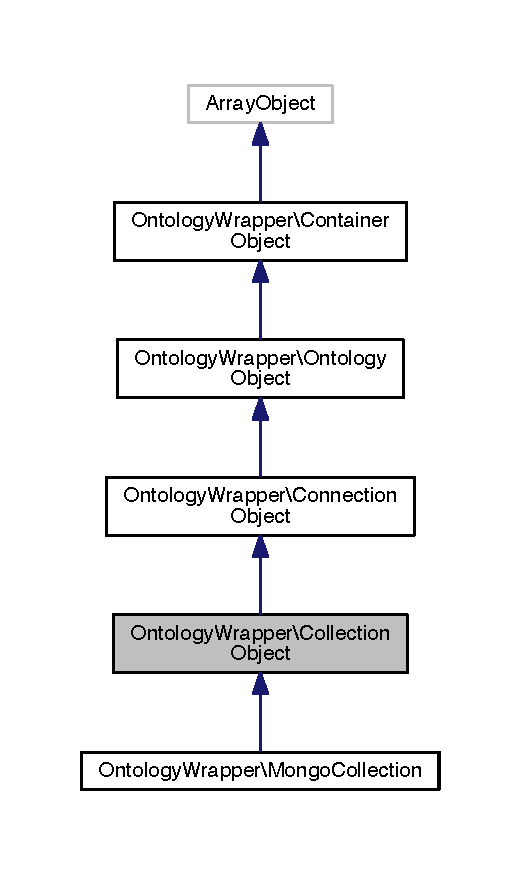
\includegraphics[width=250pt]{class_ontology_wrapper_1_1_collection_object__inherit__graph}
\end{center}
\end{figure}


Collaboration diagram for Ontology\-Wrapper\textbackslash{}Collection\-Object\-:\nopagebreak
\begin{figure}[H]
\begin{center}
\leavevmode
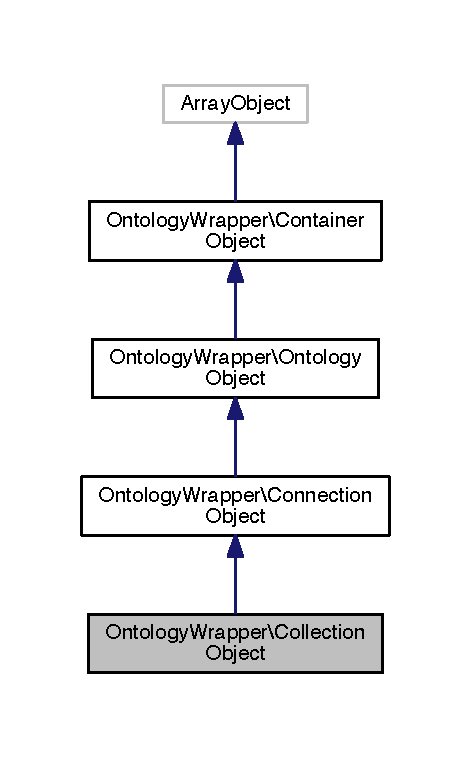
\includegraphics[width=226pt]{class_ontology_wrapper_1_1_collection_object__coll__graph}
\end{center}
\end{figure}
\subsection*{Public Member Functions}
\begin{DoxyCompactItemize}
\item 
\hyperlink{class_ontology_wrapper_1_1_collection_object_a293d59b759d71c809a626cfd5371240f}{\-\_\-\-\_\-construct} (\$the\-Parameter=N\-U\-L\-L, \$the\-Parent=N\-U\-L\-L)
\item 
\hyperlink{class_ontology_wrapper_1_1_collection_object_aee9026b21f08ac0fcfb16f093a9f3235}{drop} ()
\item 
\hyperlink{class_ontology_wrapper_1_1_collection_object_adc0a8dd83621a9d68d005b2858112c74}{insert} (\&\$the\-Object, \$the\-Options=Array())
\item 
\hyperlink{class_ontology_wrapper_1_1_collection_object_a2e6eea553a4b562445ca2959df8d170c}{resolve} (\$the\-Identifier, \$the\-Offset=k\-T\-A\-G\-\_\-\-N\-I\-D, \$as\-Object=T\-R\-U\-E)
\item 
\hyperlink{class_ontology_wrapper_1_1_collection_object_a0868032610dd81c923f4a887ec46104d}{set\-Sequence\-Number} (\$the\-Sequence, \$the\-Number=1)
\item 
\hyperlink{class_ontology_wrapper_1_1_collection_object_a17487ff9e82b493434a074c787262df0}{get\-Sequence\-Number} (\$the\-Sequence)
\end{DoxyCompactItemize}
\subsection*{Static Public Attributes}
\begin{DoxyCompactItemize}
\item 
\hypertarget{class_ontology_wrapper_1_1_collection_object_a27abf14ffa8185f0fb69b6166869ffd9}{static {\bfseries \$s\-Offsets} = array( k\-T\-A\-G\-\_\-\-C\-O\-N\-N\-\_\-\-C\-O\-L\-L )}\label{class_ontology_wrapper_1_1_collection_object_a27abf14ffa8185f0fb69b6166869ffd9}

\end{DoxyCompactItemize}
\subsection*{Protected Member Functions}
\begin{DoxyCompactItemize}
\item 
\hyperlink{class_ontology_wrapper_1_1_collection_object_a32ad8e11098caeae5498b5bc5ec74b80}{new\-Database} (\$the\-Parameter)
\item 
\hyperlink{class_ontology_wrapper_1_1_collection_object_adc48ee44a9d36d23a9db87a8ab4e4eff}{insert\-Data} (\&\$the\-Data, \&\$the\-Options)
\end{DoxyCompactItemize}
\subsection*{Additional Inherited Members}


\subsection{Detailed Description}
Collection object

This {\itshape abstract} class is the ancestor of all classes representing database collection instances, this class extends the \hyperlink{class_ontology_wrapper_1_1_connection_object}{Connection\-Object} class to implement collection specific functionality prototypes. \begin{DoxyVerb} @author            Milko A. Škofič <m.skofic@cgiar.org>
 @version   1.00 06/02/2014\end{DoxyVerb}
 

\subsection{Constructor \& Destructor Documentation}
\hypertarget{class_ontology_wrapper_1_1_collection_object_a293d59b759d71c809a626cfd5371240f}{\index{Ontology\-Wrapper\-::\-Collection\-Object@{Ontology\-Wrapper\-::\-Collection\-Object}!\-\_\-\-\_\-construct@{\-\_\-\-\_\-construct}}
\index{\-\_\-\-\_\-construct@{\-\_\-\-\_\-construct}!OntologyWrapper::CollectionObject@{Ontology\-Wrapper\-::\-Collection\-Object}}
\subsubsection[{\-\_\-\-\_\-construct}]{\setlength{\rightskip}{0pt plus 5cm}Ontology\-Wrapper\textbackslash{}\-Collection\-Object\-::\-\_\-\-\_\-construct (
\begin{DoxyParamCaption}
\item[{}]{\$the\-Parameter = {\ttfamily NULL}, }
\item[{}]{\$the\-Parent = {\ttfamily NULL}}
\end{DoxyParamCaption}
)}}\label{class_ontology_wrapper_1_1_collection_object_a293d59b759d71c809a626cfd5371240f}
Instantiate class.

We overload the constructor to instantiate a database from the provided parameter if the parent object was not provided.


\begin{DoxyParams}[1]{Parameters}
mixed & {\em \$the\-Parameter} & Data source name or parameters. \\
\hline
\hyperlink{class_ontology_wrapper_1_1_connection_object}{Connection\-Object} & {\em \$the\-Parent} & Connection parent.\\
\hline
\end{DoxyParams}
public

\begin{DoxySeeAlso}{See Also}
Server\-Object\-::\$s\-Offsets Database\-Object\-::\$s\-Offsets
\end{DoxySeeAlso}
\hyperlink{class_ontology_wrapper_1_1_collection_object_a32ad8e11098caeae5498b5bc5ec74b80}{new\-Database()} 

\subsection{Member Function Documentation}
\hypertarget{class_ontology_wrapper_1_1_collection_object_aee9026b21f08ac0fcfb16f093a9f3235}{\index{Ontology\-Wrapper\-::\-Collection\-Object@{Ontology\-Wrapper\-::\-Collection\-Object}!drop@{drop}}
\index{drop@{drop}!OntologyWrapper::CollectionObject@{Ontology\-Wrapper\-::\-Collection\-Object}}
\subsubsection[{drop}]{\setlength{\rightskip}{0pt plus 5cm}Ontology\-Wrapper\textbackslash{}\-Collection\-Object\-::drop (
\begin{DoxyParamCaption}
{}
\end{DoxyParamCaption}
)\hspace{0.3cm}{\ttfamily [abstract]}}}\label{class_ontology_wrapper_1_1_collection_object_aee9026b21f08ac0fcfb16f093a9f3235}
Drop the collection

This method should drop the current collection.

public \hypertarget{class_ontology_wrapper_1_1_collection_object_a17487ff9e82b493434a074c787262df0}{\index{Ontology\-Wrapper\-::\-Collection\-Object@{Ontology\-Wrapper\-::\-Collection\-Object}!get\-Sequence\-Number@{get\-Sequence\-Number}}
\index{get\-Sequence\-Number@{get\-Sequence\-Number}!OntologyWrapper::CollectionObject@{Ontology\-Wrapper\-::\-Collection\-Object}}
\subsubsection[{get\-Sequence\-Number}]{\setlength{\rightskip}{0pt plus 5cm}Ontology\-Wrapper\textbackslash{}\-Collection\-Object\-::get\-Sequence\-Number (
\begin{DoxyParamCaption}
\item[{}]{\$the\-Sequence}
\end{DoxyParamCaption}
)}}\label{class_ontology_wrapper_1_1_collection_object_a17487ff9e82b493434a074c787262df0}
Return sequence number

This method should return a sequence number associated to the provided parameter. This operation is equivalent to requesting an auto-\/number for a database.

Each time a sequence number is requested, the sequence seed is updated, so use this method only when the sequence is required.

If the sequence selector is not found, a new one will be created starting with the number {\ttfamily 1}, so, if you need to start with another number, use the \hyperlink{class_ontology_wrapper_1_1_collection_object_a0868032610dd81c923f4a887ec46104d}{set\-Sequence\-Number()} before.

This method is intended to be handled by database objects, in this class we simply let the object's parent, a database, perform the action.

Derived classes should never need to overload this method.


\begin{DoxyParams}[1]{Parameters}
string & {\em \$the\-Sequence} & Sequence selector.\\
\hline
\end{DoxyParams}
public \begin{DoxyReturn}{Returns}
integer Sequence number. 
\end{DoxyReturn}
\hypertarget{class_ontology_wrapper_1_1_collection_object_adc0a8dd83621a9d68d005b2858112c74}{\index{Ontology\-Wrapper\-::\-Collection\-Object@{Ontology\-Wrapper\-::\-Collection\-Object}!insert@{insert}}
\index{insert@{insert}!OntologyWrapper::CollectionObject@{Ontology\-Wrapper\-::\-Collection\-Object}}
\subsubsection[{insert}]{\setlength{\rightskip}{0pt plus 5cm}Ontology\-Wrapper\textbackslash{}\-Collection\-Object\-::insert (
\begin{DoxyParamCaption}
\item[{\&}]{\$the\-Object, }
\item[{}]{\$the\-Options = {\ttfamily Array()}}
\end{DoxyParamCaption}
)}}\label{class_ontology_wrapper_1_1_collection_object_adc0a8dd83621a9d68d005b2858112c74}
Insert an object

The method expects the provided parameter to be either an array or an \hyperlink{}{Array\-Object} instance.

The method will call the virtual \hyperlink{class_ontology_wrapper_1_1_collection_object_adc48ee44a9d36d23a9db87a8ab4e4eff}{insert\-Data()} method, passing the received object to it, which will perform the actual insert.

The method will return the inserted object's identifier, \hyperlink{}{k\-T\-A\-G\-\_\-\-N\-I\-D}.

This method will also take care of setting the \hyperlink{}{k\-T\-A\-G\-\_\-\-C\-L\-A\-S\-S} offset.


\begin{DoxyParams}[1]{Parameters}
reference & {\em \$the\-Object} & Object to insert. \\
\hline
array & {\em \$the\-Options} & Insert options.\\
\hline
\end{DoxyParams}
public \begin{DoxyReturn}{Returns}
mixed Inserted object identifier.
\end{DoxyReturn}

\begin{DoxyExceptions}{Exceptions}
{\em Exception} & \\
\hline
\end{DoxyExceptions}
\begin{DoxySeeAlso}{See Also}
k\-T\-A\-G\-\_\-\-C\-L\-A\-S\-S
\end{DoxySeeAlso}
\hyperlink{class_ontology_wrapper_1_1_connection_object_abfd8e3b96ce288b2d1b1e586e8e7172a}{is\-Connected()}  \hyperlink{class_ontology_wrapper_1_1_collection_object_adc48ee44a9d36d23a9db87a8ab4e4eff}{insert\-Data()} \hypertarget{class_ontology_wrapper_1_1_collection_object_adc48ee44a9d36d23a9db87a8ab4e4eff}{\index{Ontology\-Wrapper\-::\-Collection\-Object@{Ontology\-Wrapper\-::\-Collection\-Object}!insert\-Data@{insert\-Data}}
\index{insert\-Data@{insert\-Data}!OntologyWrapper::CollectionObject@{Ontology\-Wrapper\-::\-Collection\-Object}}
\subsubsection[{insert\-Data}]{\setlength{\rightskip}{0pt plus 5cm}Ontology\-Wrapper\textbackslash{}\-Collection\-Object\-::insert\-Data (
\begin{DoxyParamCaption}
\item[{\&}]{\$the\-Data, }
\item[{\&}]{\$the\-Options}
\end{DoxyParamCaption}
)\hspace{0.3cm}{\ttfamily [abstract]}, {\ttfamily [protected]}}}\label{class_ontology_wrapper_1_1_collection_object_adc48ee44a9d36d23a9db87a8ab4e4eff}
Insert provided data

This method should be implemented by concrete derived classes, it should insert a new record in the current collection featuring the provided data and return the record identifier.

Derived classes must implement this method.


\begin{DoxyParams}[1]{Parameters}
reference & {\em \$the\-Data} & Data to insert. \\
\hline
array & {\em \$the\-Options} & Insert options.\\
\hline
\end{DoxyParams}
protected \begin{DoxyReturn}{Returns}
mixed Object identifier. 
\end{DoxyReturn}
\hypertarget{class_ontology_wrapper_1_1_collection_object_a32ad8e11098caeae5498b5bc5ec74b80}{\index{Ontology\-Wrapper\-::\-Collection\-Object@{Ontology\-Wrapper\-::\-Collection\-Object}!new\-Database@{new\-Database}}
\index{new\-Database@{new\-Database}!OntologyWrapper::CollectionObject@{Ontology\-Wrapper\-::\-Collection\-Object}}
\subsubsection[{new\-Database}]{\setlength{\rightskip}{0pt plus 5cm}Ontology\-Wrapper\textbackslash{}\-Collection\-Object\-::new\-Database (
\begin{DoxyParamCaption}
\item[{}]{\$the\-Parameter}
\end{DoxyParamCaption}
)\hspace{0.3cm}{\ttfamily [abstract]}, {\ttfamily [protected]}}}\label{class_ontology_wrapper_1_1_collection_object_a32ad8e11098caeae5498b5bc5ec74b80}
Return a new database instance

This method should be implemented by concrete derived classes, it expects a list of offsets or a data source name containing the necessary elements to instantiate a \hyperlink{class_ontology_wrapper_1_1_database_object}{Database\-Object} instance which will be considered the current object's parent.

Note that these parameters must also include the \hyperlink{class_ontology_wrapper_1_1_server_object}{Server\-Object} parameters.

Derived classes must implement this method.


\begin{DoxyParams}[1]{Parameters}
mixed & {\em \$the\-Parameter} & Database parameters.\\
\hline
\end{DoxyParams}
protected \begin{DoxyReturn}{Returns}
\hyperlink{class_ontology_wrapper_1_1_database_object}{Database\-Object} Database instance. 
\end{DoxyReturn}
\hypertarget{class_ontology_wrapper_1_1_collection_object_a2e6eea553a4b562445ca2959df8d170c}{\index{Ontology\-Wrapper\-::\-Collection\-Object@{Ontology\-Wrapper\-::\-Collection\-Object}!resolve@{resolve}}
\index{resolve@{resolve}!OntologyWrapper::CollectionObject@{Ontology\-Wrapper\-::\-Collection\-Object}}
\subsubsection[{resolve}]{\setlength{\rightskip}{0pt plus 5cm}Ontology\-Wrapper\textbackslash{}\-Collection\-Object\-::resolve (
\begin{DoxyParamCaption}
\item[{}]{\$the\-Identifier, }
\item[{}]{\$the\-Offset = {\ttfamily kTAG\-\_\-NID}, }
\item[{}]{\$as\-Object = {\ttfamily TRUE}}
\end{DoxyParamCaption}
)\hspace{0.3cm}{\ttfamily [abstract]}}}\label{class_ontology_wrapper_1_1_collection_object_a2e6eea553a4b562445ca2959df8d170c}
Resolve an object

This method should select an object in the current collection matching the provided native identifier with the provided offset and return either the object, if the second parameter is {\ttfamily T\-R\-U\-E}, or an array if {\ttfamily F\-A\-L\-S\-E}; if the object cannot be resolved, the method should return {\ttfamily N\-U\-L\-L}.

If there are more than one objects selected, this method should only return the first.

Concrete derived classes should implement this method.


\begin{DoxyParams}[1]{Parameters}
mixed & {\em \$the\-Identifier} & Object identifier. \\
\hline
mixed & {\em \$the\-Offset} & Offset. \\
\hline
boolean & {\em \$as\-Object} & Return object if {\ttfamily T\-R\-U\-E}.\\
\hline
\end{DoxyParams}
public \begin{DoxyReturn}{Returns}
mixed Found object, array, or {\ttfamily N\-U\-L\-L}. 
\end{DoxyReturn}
\hypertarget{class_ontology_wrapper_1_1_collection_object_a0868032610dd81c923f4a887ec46104d}{\index{Ontology\-Wrapper\-::\-Collection\-Object@{Ontology\-Wrapper\-::\-Collection\-Object}!set\-Sequence\-Number@{set\-Sequence\-Number}}
\index{set\-Sequence\-Number@{set\-Sequence\-Number}!OntologyWrapper::CollectionObject@{Ontology\-Wrapper\-::\-Collection\-Object}}
\subsubsection[{set\-Sequence\-Number}]{\setlength{\rightskip}{0pt plus 5cm}Ontology\-Wrapper\textbackslash{}\-Collection\-Object\-::set\-Sequence\-Number (
\begin{DoxyParamCaption}
\item[{}]{\$the\-Sequence, }
\item[{}]{\$the\-Number = {\ttfamily 1}}
\end{DoxyParamCaption}
)}}\label{class_ontology_wrapper_1_1_collection_object_a0868032610dd81c923f4a887ec46104d}
Set sequence number

This method should initialise a sequence number associated to the provided parameter. This operation is equivalent to resetting an auto-\/number for a database.

Once the sequence is set, the next requested sequence number will hold the value set by this method, so to start counting from {\ttfamily 1} you should provide this value to this method.

This method is intended to be handled by database objects, in this class we simply let the object's parent, a database, perform the action.

Derived classes should never need to overload this method.


\begin{DoxyParams}[1]{Parameters}
string & {\em \$the\-Sequence} & Sequence selector. \\
\hline
integer & {\em \$the\-Number} & Sequence number.\\
\hline
\end{DoxyParams}
public


\begin{DoxyExceptions}{Exceptions}
{\em Exception} & \\
\hline
\end{DoxyExceptions}


The documentation for this class was generated from the following file\-:\begin{DoxyCompactItemize}
\item 
/\-Library/\-Web\-Server/\-Library/\-Ontology\-Wrapper/\-Library/\-Ontology\-Wrapper/Collection\-Object.\-php\end{DoxyCompactItemize}

\hypertarget{class_ontology_wrapper_1_1_connection_object}{\section{Ontology\-Wrapper\textbackslash{}Connection\-Object Class Reference}
\label{class_ontology_wrapper_1_1_connection_object}\index{Ontology\-Wrapper\textbackslash{}\-Connection\-Object@{Ontology\-Wrapper\textbackslash{}\-Connection\-Object}}
}


Inheritance diagram for Ontology\-Wrapper\textbackslash{}Connection\-Object\-:\nopagebreak
\begin{figure}[H]
\begin{center}
\leavevmode
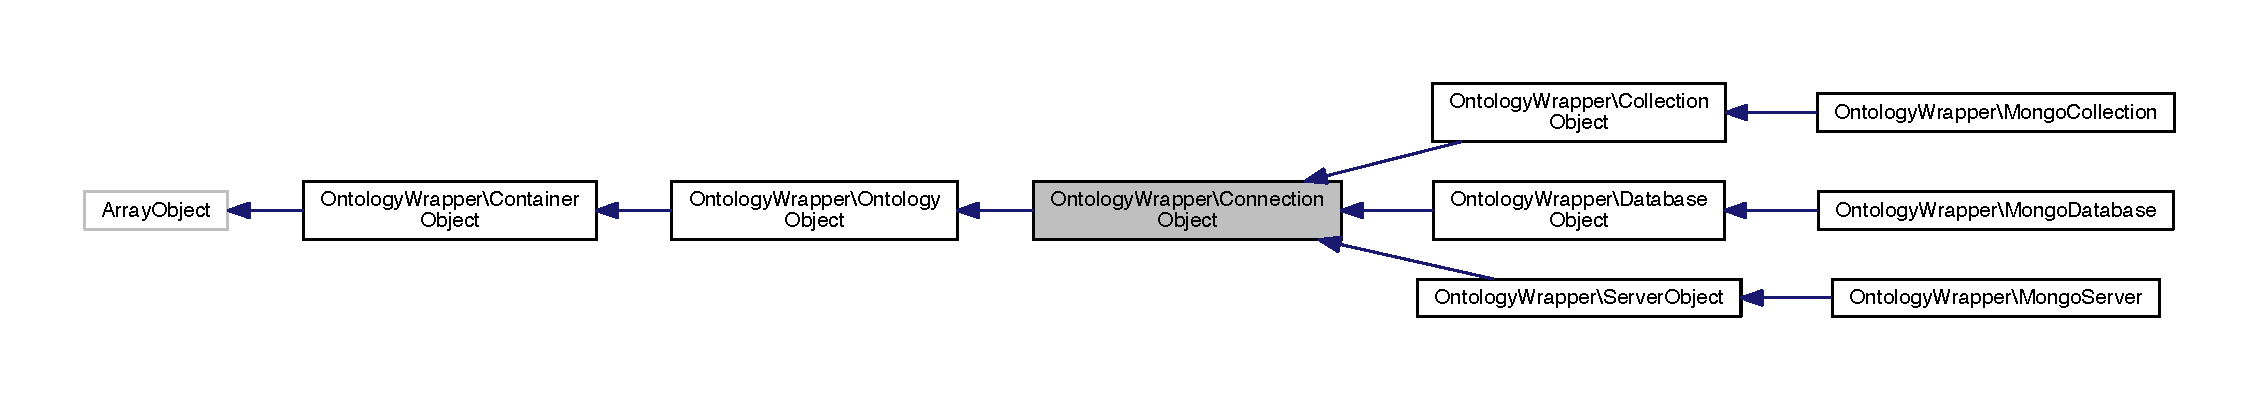
\includegraphics[width=350pt]{class_ontology_wrapper_1_1_connection_object__inherit__graph}
\end{center}
\end{figure}


Collaboration diagram for Ontology\-Wrapper\textbackslash{}Connection\-Object\-:\nopagebreak
\begin{figure}[H]
\begin{center}
\leavevmode
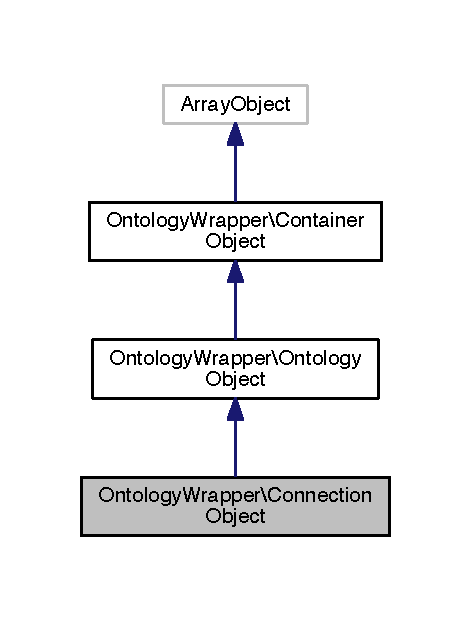
\includegraphics[width=226pt]{class_ontology_wrapper_1_1_connection_object__coll__graph}
\end{center}
\end{figure}
\subsection*{Public Member Functions}
\begin{DoxyCompactItemize}
\item 
\hyperlink{class_ontology_wrapper_1_1_connection_object_a42c5c7a5376f3e795b6dcd2cec53c429}{\-\_\-\-\_\-construct} (\$the\-Parameter=N\-U\-L\-L, \$the\-Parent=N\-U\-L\-L)
\item 
\hyperlink{class_ontology_wrapper_1_1_connection_object_a129e5d78f1d2e4b1d0e866a604d6e34c}{\-\_\-\-\_\-destruct} ()
\item 
\hyperlink{class_ontology_wrapper_1_1_connection_object_a667dca54383faee6ee734ba2109c0b52}{\-\_\-\-\_\-sleep} ()
\item 
\hyperlink{class_ontology_wrapper_1_1_connection_object_a18db4f7ebb47a4c51b4b3483314c14a9}{\-\_\-\-\_\-wakeup} ()
\item 
\hyperlink{class_ontology_wrapper_1_1_connection_object_ad7fbc642081f429ca17ffef94880d865}{\-\_\-\-\_\-to\-String} ()
\item 
\hyperlink{class_ontology_wrapper_1_1_connection_object_a9a013bdb9589e847926d196de62e87e3}{D\-S\-N} (\$the\-Value=N\-U\-L\-L, \$get\-Old=F\-A\-L\-S\-E, \$do\-Sync=T\-R\-U\-E)
\item 
\hyperlink{class_ontology_wrapper_1_1_connection_object_aeffe3ba284ae71caacaab38b3c80d345}{Connection} ()
\item 
\hyperlink{class_ontology_wrapper_1_1_connection_object_aebe90e0304d983af0f695b706120e62c}{Parent} ()
\item 
\hyperlink{class_ontology_wrapper_1_1_connection_object_abfd8e3b96ce288b2d1b1e586e8e7172a}{is\-Connected} ()
\item 
\hyperlink{class_ontology_wrapper_1_1_connection_object_aa65904a3e38f1b04cdea1d88dd80793b}{open\-Connection} ()
\item 
\hyperlink{class_ontology_wrapper_1_1_connection_object_abfff262a446ab3dc404e4132ee195430}{close\-Connection} ()
\end{DoxyCompactItemize}
\subsection*{Protected Member Functions}
\begin{DoxyCompactItemize}
\item 
\hyperlink{class_ontology_wrapper_1_1_connection_object_a8533629374db92c93b6500c5cd7b89fa}{connection\-Open} ()
\item 
\hyperlink{class_ontology_wrapper_1_1_connection_object_aa355abbd5de052f9587296c68dd98ee4}{connection\-Close} ()
\item 
\hyperlink{class_ontology_wrapper_1_1_connection_object_a3b5e9ba7510b52d1f3f3cb1971491c53}{parse\-D\-S\-N} (\$the\-D\-S\-N)
\item 
\hyperlink{class_ontology_wrapper_1_1_connection_object_aa9e833d63b5ba46bb694292e3cd7e957}{parse\-Offsets} (\$the\-Offsets)
\item 
\hyperlink{class_ontology_wrapper_1_1_connection_object_ad346cdcd5a06513ed3ae434791f9b027}{parse\-Offset} (\&\$the\-Parameters, \$the\-Offset, \$the\-Value)
\item 
\hyperlink{class_ontology_wrapper_1_1_connection_object_a25920bb50adac434b6e43b5702a85a84}{parse\-Option} (\&\$the\-Parameters, \$the\-Option, \$the\-Value)
\item 
\hyperlink{class_ontology_wrapper_1_1_connection_object_ac0e6ea1c27ccfbf1366f8c6ab8c830c7}{load\-D\-S\-N\-Parameter} (\&\$the\-Parameters, \$the\-Key, \$the\-Value=N\-U\-L\-L)
\item 
\hyperlink{class_ontology_wrapper_1_1_connection_object_a4cd98d80db32b7bddfe1e46c0239b9e0}{pre\-Offset\-Set} (\&\$the\-Offset, \&\$the\-Value)
\item 
\hyperlink{class_ontology_wrapper_1_1_connection_object_aed704c5a7f4abb5eaa96123b4c889409}{post\-Offset\-Set} (\&\$the\-Offset, \&\$the\-Value)
\item 
\hyperlink{class_ontology_wrapper_1_1_connection_object_a5d8ba718e827507c25aedda8af50d235}{pre\-Offset\-Unset} (\&\$the\-Offset)
\item 
\hyperlink{class_ontology_wrapper_1_1_connection_object_a10e24985e878fe6a15c40dcaf266e3c2}{post\-Offset\-Unset} (\&\$the\-Offset)
\end{DoxyCompactItemize}
\subsection*{Protected Attributes}
\begin{DoxyCompactItemize}
\item 
\hypertarget{class_ontology_wrapper_1_1_connection_object_a0d8f152694cf10d430028a25c1e981d3}{{\bfseries \$m\-D\-S\-N} = N\-U\-L\-L}\label{class_ontology_wrapper_1_1_connection_object_a0d8f152694cf10d430028a25c1e981d3}

\item 
\hypertarget{class_ontology_wrapper_1_1_connection_object_a1f0e856afbac9b6dc303d0365993ea78}{{\bfseries \$m\-Parent} = N\-U\-L\-L}\label{class_ontology_wrapper_1_1_connection_object_a1f0e856afbac9b6dc303d0365993ea78}

\item 
\hypertarget{class_ontology_wrapper_1_1_connection_object_a58126a003936b52fd4fbb69415bd66e4}{{\bfseries \$m\-Connection} = N\-U\-L\-L}\label{class_ontology_wrapper_1_1_connection_object_a58126a003936b52fd4fbb69415bd66e4}

\end{DoxyCompactItemize}
\subsection*{Additional Inherited Members}


\subsection{Detailed Description}
Connection object

This {\itshape abstract} class is the ancestor of all classes representing connection instances, such as servers, databases and collections.

The main purpose of this class is to wrap a common interface around concrete instances of specific server, database or collection or engines.

The class features the following properties\-:


\begin{DoxyItemize}
\item {\ttfamily \hyperlink{}{\$m\-D\-S\-N}}\-: The {\itshape data source name}, it is an U\-R\-L that represents the connection string. 
\item {\ttfamily \hyperlink{}{\$m\-Connection}}\-: The {\itshape connection resource}, it represents the native connection. 
\item {\ttfamily \hyperlink{}{\$m\-Parent}}\-: The {\itshape parent connection}, it represents the instance derived from this class that instantiated the current object. 
\end{DoxyItemize}

The object is instantiated by providing a parameter that may either be a connection U\-R\-L, such as a string that may be parsed by the \hyperlink{}{parse\-\_\-url()} function, or an array containing the connection parameters.

The public interface of this class, as well as for many other abstract classes, is implemented as templates in which protected methods do the actual work, so derived concrete classes should only need to implement the protected interface.

This class declares three methods for managing the connection\-:


\begin{DoxyItemize}
\item {\ttfamily \hyperlink{class_ontology_wrapper_1_1_connection_object_abfd8e3b96ce288b2d1b1e586e8e7172a}{is\-Connected()}}\-: Returns {\ttfamily T\-R\-U\-E} if the connection is open. 
\item {\ttfamily \hyperlink{class_ontology_wrapper_1_1_connection_object_aa65904a3e38f1b04cdea1d88dd80793b}{open\-Connection()}}\-: Create and open the connection. 
\item {\ttfamily \hyperlink{class_ontology_wrapper_1_1_connection_object_abfff262a446ab3dc404e4132ee195430}{close\-Connection()}}\-: Close and reset the connection. 
\end{DoxyItemize}

When the object goes out of context it will close the connection, if open, and re-\/open it once it gets back into context\-:


\begin{DoxyItemize}
\item {\ttfamily \hyperlink{class_ontology_wrapper_1_1_connection_object_a667dca54383faee6ee734ba2109c0b52}{\-\_\-\-\_\-sleep()}}\-: This method will close the connection, if open, and set the \hyperlink{}{connection} property to {\ttfamily T\-R\-U\-E} as an indication that the connection must be opened once the object gets back into scope. 
\item {\ttfamily \hyperlink{class_ontology_wrapper_1_1_connection_object_a18db4f7ebb47a4c51b4b3483314c14a9}{\-\_\-\-\_\-wakeup()}}\-: This method will open the connection, if the object went out of scope while the connection was open. 
\end{DoxyItemize}

The class provides accessor methods for the object properties\-: the \hyperlink{}{\$m\-D\-S\-N} data member can be managed with the \hyperlink{class_ontology_wrapper_1_1_connection_object_a9a013bdb9589e847926d196de62e87e3}{D\-S\-N()} method, the \hyperlink{}{\$m\-Connection} data member can be retrieved with the \hyperlink{class_ontology_wrapper_1_1_connection_object_aeffe3ba284ae71caacaab38b3c80d345}{Connection()} method and the \hyperlink{}{\$m\-Parent} data member can be retrieved with the \hyperlink{class_ontology_wrapper_1_1_connection_object_aebe90e0304d983af0f695b706120e62c}{Parent()} method.

When setting the connection string, \hyperlink{class_ontology_wrapper_1_1_connection_object_a9a013bdb9589e847926d196de62e87e3}{D\-S\-N()}, the object's connection parameters will be synchronised. When setting offsets, the data source name will not be changed. When the connection is opened, \hyperlink{class_ontology_wrapper_1_1_connection_object_aa65904a3e38f1b04cdea1d88dd80793b}{open\-Connection()}, the data source name will be re-\/constituted using the object's offsets. This means that the object offsets represent the actual connection parameters, although setting the D\-S\-N will reset these parameters to match the connection U\-R\-L.

When the connection is \hyperlink{class_ontology_wrapper_1_1_connection_object_abfd8e3b96ce288b2d1b1e586e8e7172a}{open}, any attempt to modify the object offsets will raise an exception\-: this is to prevent changing the connection properties while connected.

In this class we make use of the \hyperlink{}{Status} trait, here we set the \hyperlink{}{is\-Dirty()} flag whenever we modify an object offset, and we reset it whenever we open the connection; we reset the status bitfield data member after calling the parent constructor.

This object represents the building block for all concrete instances that represent servers, databases, data collections and caches.
\begin{DoxyItemize}
\item 
\item When parsing the data source name, using the \hyperlink{}{parse\-\_\-url()} function,, this class will perform the following associations\-:


\begin{DoxyItemize}
\item {\ttfamily scheme}\-: {\ttfamily \hyperlink{}{k\-T\-A\-G\-\_\-\-C\-O\-N\-N\-\_\-\-P\-R\-O\-T\-O\-C\-O\-L}}. This corresponds to the server and database protocols, which must be the same. 
\item {\ttfamily host}\-: {\ttfamily \hyperlink{}{k\-T\-A\-G\-\_\-\-C\-O\-N\-N\-\_\-\-H\-O\-S\-T}}. This corresponds to the server object connection host. 
\item {\ttfamily port}\-: {\ttfamily \hyperlink{}{k\-T\-A\-G\-\_\-\-C\-O\-N\-N\-\_\-\-P\-O\-R\-T}}. This corresponds to the server object connection port. 
\item {\ttfamily user}\-: {\ttfamily \hyperlink{}{k\-T\-A\-G\-\_\-\-C\-O\-N\-N\-\_\-\-U\-S\-E\-R}}. This corresponds to the server object connection user code. 
\item {\ttfamily pass}\-: {\ttfamily \hyperlink{}{k\-T\-A\-G\-\_\-\-C\-O\-N\-N\-\_\-\-P\-A\-S\-S}}. This corresponds to the server object connection user password. 
\item {\ttfamily path}\-: {\ttfamily \hyperlink{}{k\-T\-A\-G\-\_\-\-C\-O\-N\-N\-\_\-\-B\-A\-S\-E}}. This corresponds to the database object name. 
\item {\ttfamily fragment}\-: {\ttfamily \hyperlink{}{k\-T\-A\-G\-\_\-\-C\-O\-N\-N\-\_\-\-C\-O\-L\-L}}. This corresponds to the collection object name. 
\end{DoxyItemize}

The above associations are stored in the object's offsets, which means that a collection will hold its database name and all the parameters of the server connection. \begin{DoxyVerb}  @author         Milko A. Škofič <m.skofic@cgiar.org>
  @version        1.00 16/01/2014\end{DoxyVerb}
 
\end{DoxyItemize}

\subsection{Constructor \& Destructor Documentation}
\hypertarget{class_ontology_wrapper_1_1_connection_object_a42c5c7a5376f3e795b6dcd2cec53c429}{\index{Ontology\-Wrapper\-::\-Connection\-Object@{Ontology\-Wrapper\-::\-Connection\-Object}!\-\_\-\-\_\-construct@{\-\_\-\-\_\-construct}}
\index{\-\_\-\-\_\-construct@{\-\_\-\-\_\-construct}!OntologyWrapper::ConnectionObject@{Ontology\-Wrapper\-::\-Connection\-Object}}
\subsubsection[{\-\_\-\-\_\-construct}]{\setlength{\rightskip}{0pt plus 5cm}Ontology\-Wrapper\textbackslash{}\-Connection\-Object\-::\-\_\-\-\_\-construct (
\begin{DoxyParamCaption}
\item[{}]{\$the\-Parameter = {\ttfamily NULL}, }
\item[{}]{\$the\-Parent = {\ttfamily NULL}}
\end{DoxyParamCaption}
)}}\label{class_ontology_wrapper_1_1_connection_object_a42c5c7a5376f3e795b6dcd2cec53c429}
Instantiate class.

The object may be instantiated as an empty object, by omitting both parameters; with a {\itshape data source name} in the form of a connection U\-R\-L; or by providing an array of tag/value parameters which will constitute the object's offsets.

If you provide a data source name, this must be parsable by the \hyperlink{}{parse\-\_\-url()} function, if this is not the case, you should use the parameters list.

If the first parameter was provided, the method will synchronise both the data source name and the connection parameters.

The second parameter represents the {\itshape connection parent}, it must be an instance derived from this class and will only be set by the constructor.

When overloading the constructor in derived classes you should always first call the parent method and then perform custom actions.


\begin{DoxyParams}[1]{Parameters}
mixed & {\em \$the\-Parameter} & Data source name or parameters. \\
\hline
\hyperlink{class_ontology_wrapper_1_1_connection_object}{Connection\-Object} & {\em \$the\-Parent} & Connection parent.\\
\hline
\end{DoxyParams}
public


\begin{DoxyExceptions}{Exceptions}
{\em Exception} & \hyperlink{class_ontology_wrapper_1_1_connection_object_a9a013bdb9589e847926d196de62e87e3}{D\-S\-N()}  \hyperlink{class_ontology_wrapper_1_1_connection_object_aa9e833d63b5ba46bb694292e3cd7e957}{parse\-Offsets()}  status\-Reset() \\
\hline
\end{DoxyExceptions}
\hypertarget{class_ontology_wrapper_1_1_connection_object_a129e5d78f1d2e4b1d0e866a604d6e34c}{\index{Ontology\-Wrapper\-::\-Connection\-Object@{Ontology\-Wrapper\-::\-Connection\-Object}!\-\_\-\-\_\-destruct@{\-\_\-\-\_\-destruct}}
\index{\-\_\-\-\_\-destruct@{\-\_\-\-\_\-destruct}!OntologyWrapper::ConnectionObject@{Ontology\-Wrapper\-::\-Connection\-Object}}
\subsubsection[{\-\_\-\-\_\-destruct}]{\setlength{\rightskip}{0pt plus 5cm}Ontology\-Wrapper\textbackslash{}\-Connection\-Object\-::\-\_\-\-\_\-destruct (
\begin{DoxyParamCaption}
{}
\end{DoxyParamCaption}
)}}\label{class_ontology_wrapper_1_1_connection_object_a129e5d78f1d2e4b1d0e866a604d6e34c}
Destruct instance.

The destructor will close the connection if open.

public

\hyperlink{class_ontology_wrapper_1_1_connection_object_abfff262a446ab3dc404e4132ee195430}{close\-Connection()} 

\subsection{Member Function Documentation}
\hypertarget{class_ontology_wrapper_1_1_connection_object_a667dca54383faee6ee734ba2109c0b52}{\index{Ontology\-Wrapper\-::\-Connection\-Object@{Ontology\-Wrapper\-::\-Connection\-Object}!\-\_\-\-\_\-sleep@{\-\_\-\-\_\-sleep}}
\index{\-\_\-\-\_\-sleep@{\-\_\-\-\_\-sleep}!OntologyWrapper::ConnectionObject@{Ontology\-Wrapper\-::\-Connection\-Object}}
\subsubsection[{\-\_\-\-\_\-sleep}]{\setlength{\rightskip}{0pt plus 5cm}Ontology\-Wrapper\textbackslash{}\-Connection\-Object\-::\-\_\-\-\_\-sleep (
\begin{DoxyParamCaption}
{}
\end{DoxyParamCaption}
)}}\label{class_ontology_wrapper_1_1_connection_object_a667dca54383faee6ee734ba2109c0b52}
Sleep

This method will close the connection and replace the connection resource with {\ttfamily T\-R\-U\-E} if the connection was open.

public

\hyperlink{class_ontology_wrapper_1_1_connection_object_abfd8e3b96ce288b2d1b1e586e8e7172a}{is\-Connected()}  \hyperlink{class_ontology_wrapper_1_1_connection_object_abfff262a446ab3dc404e4132ee195430}{close\-Connection()} \hypertarget{class_ontology_wrapper_1_1_connection_object_ad7fbc642081f429ca17ffef94880d865}{\index{Ontology\-Wrapper\-::\-Connection\-Object@{Ontology\-Wrapper\-::\-Connection\-Object}!\-\_\-\-\_\-to\-String@{\-\_\-\-\_\-to\-String}}
\index{\-\_\-\-\_\-to\-String@{\-\_\-\-\_\-to\-String}!OntologyWrapper::ConnectionObject@{Ontology\-Wrapper\-::\-Connection\-Object}}
\subsubsection[{\-\_\-\-\_\-to\-String}]{\setlength{\rightskip}{0pt plus 5cm}Ontology\-Wrapper\textbackslash{}\-Connection\-Object\-::\-\_\-\-\_\-to\-String (
\begin{DoxyParamCaption}
{}
\end{DoxyParamCaption}
)}}\label{class_ontology_wrapper_1_1_connection_object_ad7fbc642081f429ca17ffef94880d865}
\subparagraph*{Return connection name}

In this class we consider the data source name as the global identifier; here we return it as is, in derived classes you should be careful to shadow sensitive data.

Note that this method cannot return the {\ttfamily N\-U\-L\-L} value, which means that it cannot be used until there is a data source name for the object.

public \begin{DoxyReturn}{Returns}
string The global identifier. 
\end{DoxyReturn}
\hypertarget{class_ontology_wrapper_1_1_connection_object_a18db4f7ebb47a4c51b4b3483314c14a9}{\index{Ontology\-Wrapper\-::\-Connection\-Object@{Ontology\-Wrapper\-::\-Connection\-Object}!\-\_\-\-\_\-wakeup@{\-\_\-\-\_\-wakeup}}
\index{\-\_\-\-\_\-wakeup@{\-\_\-\-\_\-wakeup}!OntologyWrapper::ConnectionObject@{Ontology\-Wrapper\-::\-Connection\-Object}}
\subsubsection[{\-\_\-\-\_\-wakeup}]{\setlength{\rightskip}{0pt plus 5cm}Ontology\-Wrapper\textbackslash{}\-Connection\-Object\-::\-\_\-\-\_\-wakeup (
\begin{DoxyParamCaption}
{}
\end{DoxyParamCaption}
)}}\label{class_ontology_wrapper_1_1_connection_object_a18db4f7ebb47a4c51b4b3483314c14a9}
Wake up

This method will re-\/open the connection if it was closed by the \hyperlink{class_ontology_wrapper_1_1_connection_object_a667dca54383faee6ee734ba2109c0b52}{\-\_\-\-\_\-sleep()} method.

public

\hyperlink{class_ontology_wrapper_1_1_connection_object_aa65904a3e38f1b04cdea1d88dd80793b}{open\-Connection()} \hypertarget{class_ontology_wrapper_1_1_connection_object_abfff262a446ab3dc404e4132ee195430}{\index{Ontology\-Wrapper\-::\-Connection\-Object@{Ontology\-Wrapper\-::\-Connection\-Object}!close\-Connection@{close\-Connection}}
\index{close\-Connection@{close\-Connection}!OntologyWrapper::ConnectionObject@{Ontology\-Wrapper\-::\-Connection\-Object}}
\subsubsection[{close\-Connection}]{\setlength{\rightskip}{0pt plus 5cm}Ontology\-Wrapper\textbackslash{}\-Connection\-Object\-::close\-Connection (
\begin{DoxyParamCaption}
{}
\end{DoxyParamCaption}
)}}\label{class_ontology_wrapper_1_1_connection_object_abfff262a446ab3dc404e4132ee195430}
Close connection

If the connection is open, this method will close the connection and reset the \hyperlink{class_ontology_wrapper_1_1_connection_object_aeffe3ba284ae71caacaab38b3c80d345}{Connection} data member.

The method will return {\ttfamily T\-R\-U\-E} if the connection was open and {\ttfamily F\-A\-L\-S\-E} if not.

public \begin{DoxyReturn}{Returns}
boolean {\ttfamily T\-R\-U\-E} if closed, {\ttfamily F\-A\-L\-S\-E} if was closed.
\end{DoxyReturn}
\hyperlink{class_ontology_wrapper_1_1_connection_object_abfd8e3b96ce288b2d1b1e586e8e7172a}{is\-Connected()}  \hyperlink{class_ontology_wrapper_1_1_connection_object_aa355abbd5de052f9587296c68dd98ee4}{connection\-Close()} \hypertarget{class_ontology_wrapper_1_1_connection_object_aeffe3ba284ae71caacaab38b3c80d345}{\index{Ontology\-Wrapper\-::\-Connection\-Object@{Ontology\-Wrapper\-::\-Connection\-Object}!Connection@{Connection}}
\index{Connection@{Connection}!OntologyWrapper::ConnectionObject@{Ontology\-Wrapper\-::\-Connection\-Object}}
\subsubsection[{Connection}]{\setlength{\rightskip}{0pt plus 5cm}Ontology\-Wrapper\textbackslash{}\-Connection\-Object\-::\-Connection (
\begin{DoxyParamCaption}
{}
\end{DoxyParamCaption}
)}}\label{class_ontology_wrapper_1_1_connection_object_aeffe3ba284ae71caacaab38b3c80d345}
Return connection resource.

This method can be used to retrieve the {\itshape connection resource}, this method is read-\/only, since the connection resource should only be set by the object's connection methods.

The connection resource represents the native connection.

public \begin{DoxyReturn}{Returns}
mixed Connection resource.
\end{DoxyReturn}
\begin{DoxySeeAlso}{See Also}
\$m\-Connection 
\end{DoxySeeAlso}
\hypertarget{class_ontology_wrapper_1_1_connection_object_aa355abbd5de052f9587296c68dd98ee4}{\index{Ontology\-Wrapper\-::\-Connection\-Object@{Ontology\-Wrapper\-::\-Connection\-Object}!connection\-Close@{connection\-Close}}
\index{connection\-Close@{connection\-Close}!OntologyWrapper::ConnectionObject@{Ontology\-Wrapper\-::\-Connection\-Object}}
\subsubsection[{connection\-Close}]{\setlength{\rightskip}{0pt plus 5cm}Ontology\-Wrapper\textbackslash{}\-Connection\-Object\-::connection\-Close (
\begin{DoxyParamCaption}
{}
\end{DoxyParamCaption}
)\hspace{0.3cm}{\ttfamily [abstract]}, {\ttfamily [protected]}}}\label{class_ontology_wrapper_1_1_connection_object_aa355abbd5de052f9587296c68dd98ee4}
Open connection

This method should close the actual connection, in this class the method is virtual.

This method expects the caller to have checked whether the connection is open.

If the operation fails, the method should raise an exception.


\begin{DoxyParams}[1]{Parameters}
mixed & {\em \$the\-Connection} & Connection.\\
\hline
\end{DoxyParams}
protected \hypertarget{class_ontology_wrapper_1_1_connection_object_a8533629374db92c93b6500c5cd7b89fa}{\index{Ontology\-Wrapper\-::\-Connection\-Object@{Ontology\-Wrapper\-::\-Connection\-Object}!connection\-Open@{connection\-Open}}
\index{connection\-Open@{connection\-Open}!OntologyWrapper::ConnectionObject@{Ontology\-Wrapper\-::\-Connection\-Object}}
\subsubsection[{connection\-Open}]{\setlength{\rightskip}{0pt plus 5cm}Ontology\-Wrapper\textbackslash{}\-Connection\-Object\-::connection\-Open (
\begin{DoxyParamCaption}
{}
\end{DoxyParamCaption}
)\hspace{0.3cm}{\ttfamily [abstract]}, {\ttfamily [protected]}}}\label{class_ontology_wrapper_1_1_connection_object_a8533629374db92c93b6500c5cd7b89fa}
Open connection

This method should open the actual connection and set the \hyperlink{}{m\-Connection} data member; in this class the method is virtual.

This method expects the caller to have checked whether the connection is already open.

If the operation fails, the method should raise an exception.

protected \begin{DoxyReturn}{Returns}
mixed The native connection. 
\end{DoxyReturn}
\hypertarget{class_ontology_wrapper_1_1_connection_object_a9a013bdb9589e847926d196de62e87e3}{\index{Ontology\-Wrapper\-::\-Connection\-Object@{Ontology\-Wrapper\-::\-Connection\-Object}!D\-S\-N@{D\-S\-N}}
\index{D\-S\-N@{D\-S\-N}!OntologyWrapper::ConnectionObject@{Ontology\-Wrapper\-::\-Connection\-Object}}
\subsubsection[{D\-S\-N}]{\setlength{\rightskip}{0pt plus 5cm}Ontology\-Wrapper\textbackslash{}\-Connection\-Object\-::\-D\-S\-N (
\begin{DoxyParamCaption}
\item[{}]{\$the\-Value = {\ttfamily NULL}, }
\item[{}]{\$get\-Old = {\ttfamily FALSE}, }
\item[{}]{\$do\-Sync = {\ttfamily TRUE}}
\end{DoxyParamCaption}
)}}\label{class_ontology_wrapper_1_1_connection_object_a9a013bdb9589e847926d196de62e87e3}
Manage data source name

This method can be used to manage the {\itshape data source name}, it accepts a parameter which represents either the data source name or the requested operation, depending on its value\-:


\begin{DoxyItemize}
\item {\ttfamily N\-U\-L\-L}\-: Return the current value. 
\item {\ttfamily F\-A\-L\-S\-E}\-: Delete the current value. 
\item {\itshape other}\-: Set the value with the provided parameter. 
\end{DoxyItemize}

The second parameter is a boolean which if {\ttfamily T\-R\-U\-E} will return the {\itshape old} value when replacing or resetting; if {\ttfamily F\-A\-L\-S\-E}, it will return the current value.

The last parameter is a switch that determines whether the object offsets should be synchronised\-: if {\ttfamily T\-R\-U\-E}, the object offsets will be reset and populated with the elements parsed from the data source name; if {\ttfamily F\-A\-L\-S\-E}, the object offsets will not be modified. This parameter is set to {\ttfamily F\-A\-L\-S\-E} by the constructor, since using all offsets may produce an invalid U\-R\-L and is {\ttfamily T\-R\-U\-E} by default, since setting a connection U\-R\-L generally means changing the parameters.

Whenever a new value is set or the value is deleted, the method will synchronise the object offsets.


\begin{DoxyParams}[1]{Parameters}
mixed & {\em \$the\-Value} & Data source name or operation. \\
\hline
boolean & {\em \$get\-Old} & {\ttfamily T\-R\-U\-E} get old value. \\
\hline
boolean & {\em \$do\-Sync} & {\ttfamily T\-R\-U\-E} will sync offsets.\\
\hline
\end{DoxyParams}
public \begin{DoxyReturn}{Returns}
mixed {\itshape New} or {\itshape old} data source name.
\end{DoxyReturn}

\begin{DoxyExceptions}{Exceptions}
{\em Exception} & \\
\hline
\end{DoxyExceptions}
\begin{DoxySeeAlso}{See Also}
\$m\-D\-S\-N
\end{DoxySeeAlso}
\hyperlink{class_ontology_wrapper_1_1_connection_object_abfd8e3b96ce288b2d1b1e586e8e7172a}{is\-Connected()}  manage\-Property()  \hyperlink{class_ontology_wrapper_1_1_connection_object_a3b5e9ba7510b52d1f3f3cb1971491c53}{parse\-D\-S\-N()}  is\-Dirty() \hypertarget{class_ontology_wrapper_1_1_connection_object_abfd8e3b96ce288b2d1b1e586e8e7172a}{\index{Ontology\-Wrapper\-::\-Connection\-Object@{Ontology\-Wrapper\-::\-Connection\-Object}!is\-Connected@{is\-Connected}}
\index{is\-Connected@{is\-Connected}!OntologyWrapper::ConnectionObject@{Ontology\-Wrapper\-::\-Connection\-Object}}
\subsubsection[{is\-Connected}]{\setlength{\rightskip}{0pt plus 5cm}Ontology\-Wrapper\textbackslash{}\-Connection\-Object\-::is\-Connected (
\begin{DoxyParamCaption}
{}
\end{DoxyParamCaption}
)}}\label{class_ontology_wrapper_1_1_connection_object_abfd8e3b96ce288b2d1b1e586e8e7172a}
Check if connection is open

This method returns a boolean flag indicating whether the connection is open or not.

public \begin{DoxyReturn}{Returns}
boolean {\ttfamily T\-R\-U\-E} is open. 
\end{DoxyReturn}
\hypertarget{class_ontology_wrapper_1_1_connection_object_ac0e6ea1c27ccfbf1366f8c6ab8c830c7}{\index{Ontology\-Wrapper\-::\-Connection\-Object@{Ontology\-Wrapper\-::\-Connection\-Object}!load\-D\-S\-N\-Parameter@{load\-D\-S\-N\-Parameter}}
\index{load\-D\-S\-N\-Parameter@{load\-D\-S\-N\-Parameter}!OntologyWrapper::ConnectionObject@{Ontology\-Wrapper\-::\-Connection\-Object}}
\subsubsection[{load\-D\-S\-N\-Parameter}]{\setlength{\rightskip}{0pt plus 5cm}Ontology\-Wrapper\textbackslash{}\-Connection\-Object\-::load\-D\-S\-N\-Parameter (
\begin{DoxyParamCaption}
\item[{\&}]{\$the\-Parameters, }
\item[{}]{\$the\-Key, }
\item[{}]{\$the\-Value = {\ttfamily NULL}}
\end{DoxyParamCaption}
)\hspace{0.3cm}{\ttfamily [protected]}}}\label{class_ontology_wrapper_1_1_connection_object_ac0e6ea1c27ccfbf1366f8c6ab8c830c7}
Load connection parameters from D\-S\-N

This method will load the parameters parsed from the data source name into the current object's offsets, it expects three parameters\-:


\begin{DoxyItemize}
\item {\bfseries \$the\-Parameters}\-: This array is the result of the \hyperlink{}{parse\-\_\-url()} function on the data source name\-: 
\begin{DoxyItemize}
\item {\ttfamily {\ttfamily scheme}}\-: We set it in \hyperlink{}{k\-T\-A\-G\-\_\-\-C\-O\-N\-N\-\_\-\-P\-R\-O\-T\-O\-C\-O\-L}. 
\item {\ttfamily {\ttfamily host}}\-: We set it in \hyperlink{}{k\-T\-A\-G\-\_\-\-C\-O\-N\-N\-\_\-\-H\-O\-S\-T}. 
\item {\ttfamily {\ttfamily port}}\-: We set it in \hyperlink{}{k\-T\-A\-G\-\_\-\-C\-O\-N\-N\-\_\-\-P\-O\-R\-T}. 
\item {\ttfamily {\ttfamily user}}\-: We set it in \hyperlink{}{k\-T\-A\-G\-\_\-\-C\-O\-N\-N\-\_\-\-U\-S\-E\-R}. 
\item {\ttfamily {\ttfamily pass}}\-: We set it in \hyperlink{}{k\-T\-A\-G\-\_\-\-C\-O\-N\-N\-\_\-\-P\-A\-S\-S}. 
\item {\ttfamily {\ttfamily path}}\-: We set it in \hyperlink{}{k\-T\-A\-G\-\_\-\-C\-O\-N\-N\-\_\-\-B\-A\-S\-E}. 
\item {\ttfamily {\ttfamily fragment}}\-: We set it in \hyperlink{}{k\-T\-A\-G\-\_\-\-C\-O\-N\-N\-\_\-\-C\-O\-L\-L}. 
\item {\ttfamily {\ttfamily query}}\-: We load the key/value pairs into \hyperlink{}{k\-T\-A\-G\-\_\-\-C\-O\-N\-N\-\_\-\-O\-P\-T\-S} array. 
\end{DoxyItemize}
\item {\bfseries \$the\-Key}\-: This parameter represents the offset. 
\item {\bfseries \$the\-Value}\-: This parameter represents the offset value. 
\end{DoxyItemize}

This is the method that derived classes may overload to customise the parameters.


\begin{DoxyParams}[1]{Parameters}
reference & {\em \$the\-Parameters} & Original parameters list. \\
\hline
string & {\em \$the\-Key} & Parameter key. \\
\hline
string & {\em \$the\-Value} & Parameter value.\\
\hline
\end{DoxyParams}
protected \hypertarget{class_ontology_wrapper_1_1_connection_object_aa65904a3e38f1b04cdea1d88dd80793b}{\index{Ontology\-Wrapper\-::\-Connection\-Object@{Ontology\-Wrapper\-::\-Connection\-Object}!open\-Connection@{open\-Connection}}
\index{open\-Connection@{open\-Connection}!OntologyWrapper::ConnectionObject@{Ontology\-Wrapper\-::\-Connection\-Object}}
\subsubsection[{open\-Connection}]{\setlength{\rightskip}{0pt plus 5cm}Ontology\-Wrapper\textbackslash{}\-Connection\-Object\-::open\-Connection (
\begin{DoxyParamCaption}
{}
\end{DoxyParamCaption}
)}}\label{class_ontology_wrapper_1_1_connection_object_aa65904a3e38f1b04cdea1d88dd80793b}
Open connection

This method can be used to create and open the connection.

We first check if the connection is already set\-: if so we do nothing.

We call the protected \hyperlink{class_ontology_wrapper_1_1_connection_object_a8533629374db92c93b6500c5cd7b89fa}{connection\-Open()} method which will open the connection and return the connection resource which will be set in the data member, \hyperlink{}{m\-Connection}.

The method will return the connection resource.

public \begin{DoxyReturn}{Returns}
mixed Depends on implementation.
\end{DoxyReturn}
\hyperlink{class_ontology_wrapper_1_1_connection_object_abfd8e3b96ce288b2d1b1e586e8e7172a}{is\-Connected()}  is\-Dirty()  \hyperlink{class_ontology_wrapper_1_1_connection_object_a9a013bdb9589e847926d196de62e87e3}{D\-S\-N()}  \hyperlink{class_ontology_wrapper_1_1_connection_object_aa9e833d63b5ba46bb694292e3cd7e957}{parse\-Offsets()}  \hyperlink{class_ontology_wrapper_1_1_connection_object_a8533629374db92c93b6500c5cd7b89fa}{connection\-Open()} \hypertarget{class_ontology_wrapper_1_1_connection_object_aebe90e0304d983af0f695b706120e62c}{\index{Ontology\-Wrapper\-::\-Connection\-Object@{Ontology\-Wrapper\-::\-Connection\-Object}!Parent@{Parent}}
\index{Parent@{Parent}!OntologyWrapper::ConnectionObject@{Ontology\-Wrapper\-::\-Connection\-Object}}
\subsubsection[{Parent}]{\setlength{\rightskip}{0pt plus 5cm}Ontology\-Wrapper\textbackslash{}\-Connection\-Object\-::\-Parent (
\begin{DoxyParamCaption}
{}
\end{DoxyParamCaption}
)}}\label{class_ontology_wrapper_1_1_connection_object_aebe90e0304d983af0f695b706120e62c}
Return connection parent.

This method can be used to retrieve the {\itshape parent connection}, this method is read-\/only, since the connection parent can only be set by the constructor and cannot be changed once the object has been instantiated.

The connection parent represents the connection creator as the server for a database.

public \begin{DoxyReturn}{Returns}
\hyperlink{class_ontology_wrapper_1_1_connection_object}{Connection\-Object} Parent connection.
\end{DoxyReturn}
\begin{DoxySeeAlso}{See Also}
\$m\-Parent 
\end{DoxySeeAlso}
\hypertarget{class_ontology_wrapper_1_1_connection_object_a3b5e9ba7510b52d1f3f3cb1971491c53}{\index{Ontology\-Wrapper\-::\-Connection\-Object@{Ontology\-Wrapper\-::\-Connection\-Object}!parse\-D\-S\-N@{parse\-D\-S\-N}}
\index{parse\-D\-S\-N@{parse\-D\-S\-N}!OntologyWrapper::ConnectionObject@{Ontology\-Wrapper\-::\-Connection\-Object}}
\subsubsection[{parse\-D\-S\-N}]{\setlength{\rightskip}{0pt plus 5cm}Ontology\-Wrapper\textbackslash{}\-Connection\-Object\-::parse\-D\-S\-N (
\begin{DoxyParamCaption}
\item[{}]{\$the\-D\-S\-N}
\end{DoxyParamCaption}
)\hspace{0.3cm}{\ttfamily [protected]}}}\label{class_ontology_wrapper_1_1_connection_object_a3b5e9ba7510b52d1f3f3cb1971491c53}
Parse data source name

This method will parse the provided data source name, extract the connection parameters and set them in the current object.

The method will make use of the \hyperlink{}{parse\-\_\-url()} function and pass each key/value pair to the protected \hyperlink{class_ontology_wrapper_1_1_connection_object_ac0e6ea1c27ccfbf1366f8c6ab8c830c7}{load\-D\-S\-N\-Parameter()} method which has the responsibility of matching the \hyperlink{}{parse\-\_\-url()} keys to \hyperlink{class_ontology_wrapper_1_1_tag}{Tag} instances.

If the \hyperlink{}{parse\-\_\-url()} function fails to parse the D\-S\-N, the method will raise an exception.

Derived classes should overload the \hyperlink{class_ontology_wrapper_1_1_connection_object_ac0e6ea1c27ccfbf1366f8c6ab8c830c7}{load\-D\-S\-N\-Parameter()} method.


\begin{DoxyParams}[1]{Parameters}
string & {\em \$the\-D\-S\-N} & Data source name.\\
\hline
\end{DoxyParams}
protected


\begin{DoxyExceptions}{Exceptions}
{\em Exception} & \hyperlink{class_ontology_wrapper_1_1_connection_object_ac0e6ea1c27ccfbf1366f8c6ab8c830c7}{load\-D\-S\-N\-Parameter()} \\
\hline
\end{DoxyExceptions}
\hypertarget{class_ontology_wrapper_1_1_connection_object_ad346cdcd5a06513ed3ae434791f9b027}{\index{Ontology\-Wrapper\-::\-Connection\-Object@{Ontology\-Wrapper\-::\-Connection\-Object}!parse\-Offset@{parse\-Offset}}
\index{parse\-Offset@{parse\-Offset}!OntologyWrapper::ConnectionObject@{Ontology\-Wrapper\-::\-Connection\-Object}}
\subsubsection[{parse\-Offset}]{\setlength{\rightskip}{0pt plus 5cm}Ontology\-Wrapper\textbackslash{}\-Connection\-Object\-::parse\-Offset (
\begin{DoxyParamCaption}
\item[{\&}]{\$the\-Parameters, }
\item[{}]{\$the\-Offset, }
\item[{}]{\$the\-Value}
\end{DoxyParamCaption}
)\hspace{0.3cm}{\ttfamily [protected]}}}\label{class_ontology_wrapper_1_1_connection_object_ad346cdcd5a06513ed3ae434791f9b027}
Parse offset

This method will parse the provided offset and populate the provided parameters. The main duty is to load the offset values into the provided parameters array so to create the same result as the \hyperlink{}{parse\-\_\-url()} function.

The resulting array can have the following elements\-:


\begin{DoxyItemize}
\item {\ttfamily {\ttfamily scheme}}\-: The protocol or scheme. 
\item {\ttfamily {\ttfamily host}}\-: The connection host. 
\item {\ttfamily {\ttfamily port}}\-: The connection port. 
\item {\ttfamily {\ttfamily user}}\-: The user code. 
\item {\ttfamily {\ttfamily pass}}\-: The user password. 
\item {\ttfamily {\ttfamily path}}\-: The connection path. 
\item {\ttfamily {\ttfamily query}}\-: The connection options. 
\item {\ttfamily {\ttfamily fragment}}\-: The U\-R\-L fragment. 
\end{DoxyItemize}

In this class we handle the following offsets\-:


\begin{DoxyItemize}
\item {\ttfamily \hyperlink{}{k\-T\-A\-G\-\_\-\-C\-O\-N\-N\-\_\-\-P\-R\-O\-T\-O\-C\-O\-L}}\-: The {\ttfamily scheme}. 
\item {\ttfamily \hyperlink{}{k\-T\-A\-G\-\_\-\-C\-O\-N\-N\-\_\-\-H\-O\-S\-T}}\-: The connection {\ttfamily host}. 
\item {\ttfamily \hyperlink{}{k\-T\-A\-G\-\_\-\-C\-O\-N\-N\-\_\-\-P\-O\-R\-T}}\-: The connection {\ttfamily port}. 
\item {\ttfamily \hyperlink{}{k\-T\-A\-G\-\_\-\-C\-O\-N\-N\-\_\-\-U\-S\-E\-R}}\-: The {\ttfamily user} code. 
\item {\ttfamily \hyperlink{}{k\-T\-A\-G\-\_\-\-C\-O\-N\-N\-\_\-\-P\-A\-S\-S}}\-: The user {\ttfamily pass}word. 
\item {\ttfamily \hyperlink{}{k\-T\-A\-G\-\_\-\-C\-O\-N\-N\-\_\-\-B\-A\-S\-E}}\-: The user {\ttfamily path}word. 
\item {\ttfamily \hyperlink{}{k\-T\-A\-G\-\_\-\-C\-O\-N\-N\-\_\-\-C\-O\-L\-L}}\-: The user {\ttfamily fragment}word. 
\item {\ttfamily \hyperlink{}{k\-T\-A\-G\-\_\-\-C\-O\-N\-N\-\_\-\-O\-P\-T\-S}}\-: The connection options, {\ttfamily query}. 
\end{DoxyItemize}

Derived classes can overload this method to customise the parameters.


\begin{DoxyParams}[1]{Parameters}
reference & {\em \$the\-Parameters} & Receives parsed offset. \\
\hline
string & {\em \$the\-Offset} & Offset. \\
\hline
mixed & {\em \$the\-Value} & Offset value.\\
\hline
\end{DoxyParams}
protected

\hyperlink{class_ontology_wrapper_1_1_connection_object_a25920bb50adac434b6e43b5702a85a84}{parse\-Option()} \hypertarget{class_ontology_wrapper_1_1_connection_object_aa9e833d63b5ba46bb694292e3cd7e957}{\index{Ontology\-Wrapper\-::\-Connection\-Object@{Ontology\-Wrapper\-::\-Connection\-Object}!parse\-Offsets@{parse\-Offsets}}
\index{parse\-Offsets@{parse\-Offsets}!OntologyWrapper::ConnectionObject@{Ontology\-Wrapper\-::\-Connection\-Object}}
\subsubsection[{parse\-Offsets}]{\setlength{\rightskip}{0pt plus 5cm}Ontology\-Wrapper\textbackslash{}\-Connection\-Object\-::parse\-Offsets (
\begin{DoxyParamCaption}
\item[{}]{\$the\-Offsets}
\end{DoxyParamCaption}
)\hspace{0.3cm}{\ttfamily [protected]}}}\label{class_ontology_wrapper_1_1_connection_object_aa9e833d63b5ba46bb694292e3cd7e957}
Parse connection parameters

This method will parse the provided key/value array and generate a connection U\-R\-L.

The method will iterate the provided offsets and feed them to the protected \hyperlink{class_ontology_wrapper_1_1_connection_object_ad346cdcd5a06513ed3ae434791f9b027}{parse\-Offset()} method which will populate an array structured as the result of the \hyperlink{}{parse\-\_\-url()} function, it will be the duty of this method to generate a data source name from that array.

Derived classes should overload the called methods and not this one.

If the resulting data source name is empty, the method will return {\ttfamily F\-A\-L\-S\-E}.


\begin{DoxyParams}[1]{Parameters}
array & {\em \$the\-Offsets} & Offsets.\\
\hline
\end{DoxyParams}
protected \begin{DoxyReturn}{Returns}
mixed Data source name or {\ttfamily F\-A\-L\-S\-E} if empty.
\end{DoxyReturn}
\hyperlink{class_ontology_wrapper_1_1_connection_object_ad346cdcd5a06513ed3ae434791f9b027}{parse\-Offset()} \hypertarget{class_ontology_wrapper_1_1_connection_object_a25920bb50adac434b6e43b5702a85a84}{\index{Ontology\-Wrapper\-::\-Connection\-Object@{Ontology\-Wrapper\-::\-Connection\-Object}!parse\-Option@{parse\-Option}}
\index{parse\-Option@{parse\-Option}!OntologyWrapper::ConnectionObject@{Ontology\-Wrapper\-::\-Connection\-Object}}
\subsubsection[{parse\-Option}]{\setlength{\rightskip}{0pt plus 5cm}Ontology\-Wrapper\textbackslash{}\-Connection\-Object\-::parse\-Option (
\begin{DoxyParamCaption}
\item[{\&}]{\$the\-Parameters, }
\item[{}]{\$the\-Option, }
\item[{}]{\$the\-Value}
\end{DoxyParamCaption}
)\hspace{0.3cm}{\ttfamily [protected]}}}\label{class_ontology_wrapper_1_1_connection_object_a25920bb50adac434b6e43b5702a85a84}
Parse option

This method will parse the provided option and populate the query parameters. The main duty is to load the option into the {\ttfamily query} element of the provided parameters list as the result of the \hyperlink{}{parse\-\_\-url()} function.

In this class we load what we find.

Derived classes can overload this method to customise the options.


\begin{DoxyParams}[1]{Parameters}
reference & {\em \$the\-Parameters} & Receives parsed offset. \\
\hline
string & {\em \$the\-Option} & Option. \\
\hline
mixed & {\em \$the\-Value} & Option value.\\
\hline
\end{DoxyParams}
protected \hypertarget{class_ontology_wrapper_1_1_connection_object_aed704c5a7f4abb5eaa96123b4c889409}{\index{Ontology\-Wrapper\-::\-Connection\-Object@{Ontology\-Wrapper\-::\-Connection\-Object}!post\-Offset\-Set@{post\-Offset\-Set}}
\index{post\-Offset\-Set@{post\-Offset\-Set}!OntologyWrapper::ConnectionObject@{Ontology\-Wrapper\-::\-Connection\-Object}}
\subsubsection[{post\-Offset\-Set}]{\setlength{\rightskip}{0pt plus 5cm}Ontology\-Wrapper\textbackslash{}\-Connection\-Object\-::post\-Offset\-Set (
\begin{DoxyParamCaption}
\item[{\&}]{\$the\-Offset, }
\item[{\&}]{\$the\-Value}
\end{DoxyParamCaption}
)\hspace{0.3cm}{\ttfamily [protected]}}}\label{class_ontology_wrapper_1_1_connection_object_aed704c5a7f4abb5eaa96123b4c889409}
Handle offset and value after setting it

We set the \hyperlink{}{is\-Dirty()} status.


\begin{DoxyParams}[1]{Parameters}
reference & {\em \$the\-Offset} & Offset reference. \\
\hline
reference & {\em \$the\-Value} & Offset value reference.\\
\hline
\end{DoxyParams}
protected

is\-Dirty() \hypertarget{class_ontology_wrapper_1_1_connection_object_a10e24985e878fe6a15c40dcaf266e3c2}{\index{Ontology\-Wrapper\-::\-Connection\-Object@{Ontology\-Wrapper\-::\-Connection\-Object}!post\-Offset\-Unset@{post\-Offset\-Unset}}
\index{post\-Offset\-Unset@{post\-Offset\-Unset}!OntologyWrapper::ConnectionObject@{Ontology\-Wrapper\-::\-Connection\-Object}}
\subsubsection[{post\-Offset\-Unset}]{\setlength{\rightskip}{0pt plus 5cm}Ontology\-Wrapper\textbackslash{}\-Connection\-Object\-::post\-Offset\-Unset (
\begin{DoxyParamCaption}
\item[{\&}]{\$the\-Offset}
\end{DoxyParamCaption}
)\hspace{0.3cm}{\ttfamily [protected]}}}\label{class_ontology_wrapper_1_1_connection_object_a10e24985e878fe6a15c40dcaf266e3c2}
Handle offset and value after deleting it

We set the \hyperlink{}{is\-Dirty()} status.


\begin{DoxyParams}[1]{Parameters}
reference & {\em \$the\-Offset} & Offset reference. \\
\hline
reference & {\em \$the\-Value} & Offset value reference.\\
\hline
\end{DoxyParams}
protected

is\-Dirty() \hypertarget{class_ontology_wrapper_1_1_connection_object_a4cd98d80db32b7bddfe1e46c0239b9e0}{\index{Ontology\-Wrapper\-::\-Connection\-Object@{Ontology\-Wrapper\-::\-Connection\-Object}!pre\-Offset\-Set@{pre\-Offset\-Set}}
\index{pre\-Offset\-Set@{pre\-Offset\-Set}!OntologyWrapper::ConnectionObject@{Ontology\-Wrapper\-::\-Connection\-Object}}
\subsubsection[{pre\-Offset\-Set}]{\setlength{\rightskip}{0pt plus 5cm}Ontology\-Wrapper\textbackslash{}\-Connection\-Object\-::pre\-Offset\-Set (
\begin{DoxyParamCaption}
\item[{\&}]{\$the\-Offset, }
\item[{\&}]{\$the\-Value}
\end{DoxyParamCaption}
)\hspace{0.3cm}{\ttfamily [protected]}}}\label{class_ontology_wrapper_1_1_connection_object_a4cd98d80db32b7bddfe1e46c0239b9e0}
Handle offset and value before setting it

We overload this method to prevent setting values while the connection is open.


\begin{DoxyParams}[1]{Parameters}
reference & {\em \$the\-Offset} & Offset reference. \\
\hline
reference & {\em \$the\-Value} & Offset value reference.\\
\hline
\end{DoxyParams}
protected \begin{DoxyReturn}{Returns}
mixed {\ttfamily N\-U\-L\-L} set offset value, other, return.
\end{DoxyReturn}

\begin{DoxyExceptions}{Exceptions}
{\em Exception} & \hyperlink{class_ontology_wrapper_1_1_connection_object_abfd8e3b96ce288b2d1b1e586e8e7172a}{is\-Connected()} \\
\hline
\end{DoxyExceptions}
\hypertarget{class_ontology_wrapper_1_1_connection_object_a5d8ba718e827507c25aedda8af50d235}{\index{Ontology\-Wrapper\-::\-Connection\-Object@{Ontology\-Wrapper\-::\-Connection\-Object}!pre\-Offset\-Unset@{pre\-Offset\-Unset}}
\index{pre\-Offset\-Unset@{pre\-Offset\-Unset}!OntologyWrapper::ConnectionObject@{Ontology\-Wrapper\-::\-Connection\-Object}}
\subsubsection[{pre\-Offset\-Unset}]{\setlength{\rightskip}{0pt plus 5cm}Ontology\-Wrapper\textbackslash{}\-Connection\-Object\-::pre\-Offset\-Unset (
\begin{DoxyParamCaption}
\item[{\&}]{\$the\-Offset}
\end{DoxyParamCaption}
)\hspace{0.3cm}{\ttfamily [protected]}}}\label{class_ontology_wrapper_1_1_connection_object_a5d8ba718e827507c25aedda8af50d235}
Handle offset and value before deleting it

We overload this method to prevent deleting values while the connection is open.


\begin{DoxyParams}[1]{Parameters}
reference & {\em \$the\-Offset} & Offset reference.\\
\hline
\end{DoxyParams}
protected \begin{DoxyReturn}{Returns}
mixed {\ttfamily N\-U\-L\-L} delete offset value, other, return.
\end{DoxyReturn}
\hyperlink{class_ontology_wrapper_1_1_connection_object_abfd8e3b96ce288b2d1b1e586e8e7172a}{is\-Connected()} 

The documentation for this class was generated from the following file\-:\begin{DoxyCompactItemize}
\item 
/\-Library/\-Web\-Server/\-Library/\-Ontology\-Wrapper/\-Library/\-Ontology\-Wrapper/Connection\-Object.\-php\end{DoxyCompactItemize}

\hypertarget{class_ontology_wrapper_1_1_container_object}{\section{Ontology\-Wrapper\textbackslash{}Container\-Object Class Reference}
\label{class_ontology_wrapper_1_1_container_object}\index{Ontology\-Wrapper\textbackslash{}\-Container\-Object@{Ontology\-Wrapper\textbackslash{}\-Container\-Object}}
}


Inheritance diagram for Ontology\-Wrapper\textbackslash{}Container\-Object\-:
\nopagebreak
\begin{figure}[H]
\begin{center}
\leavevmode
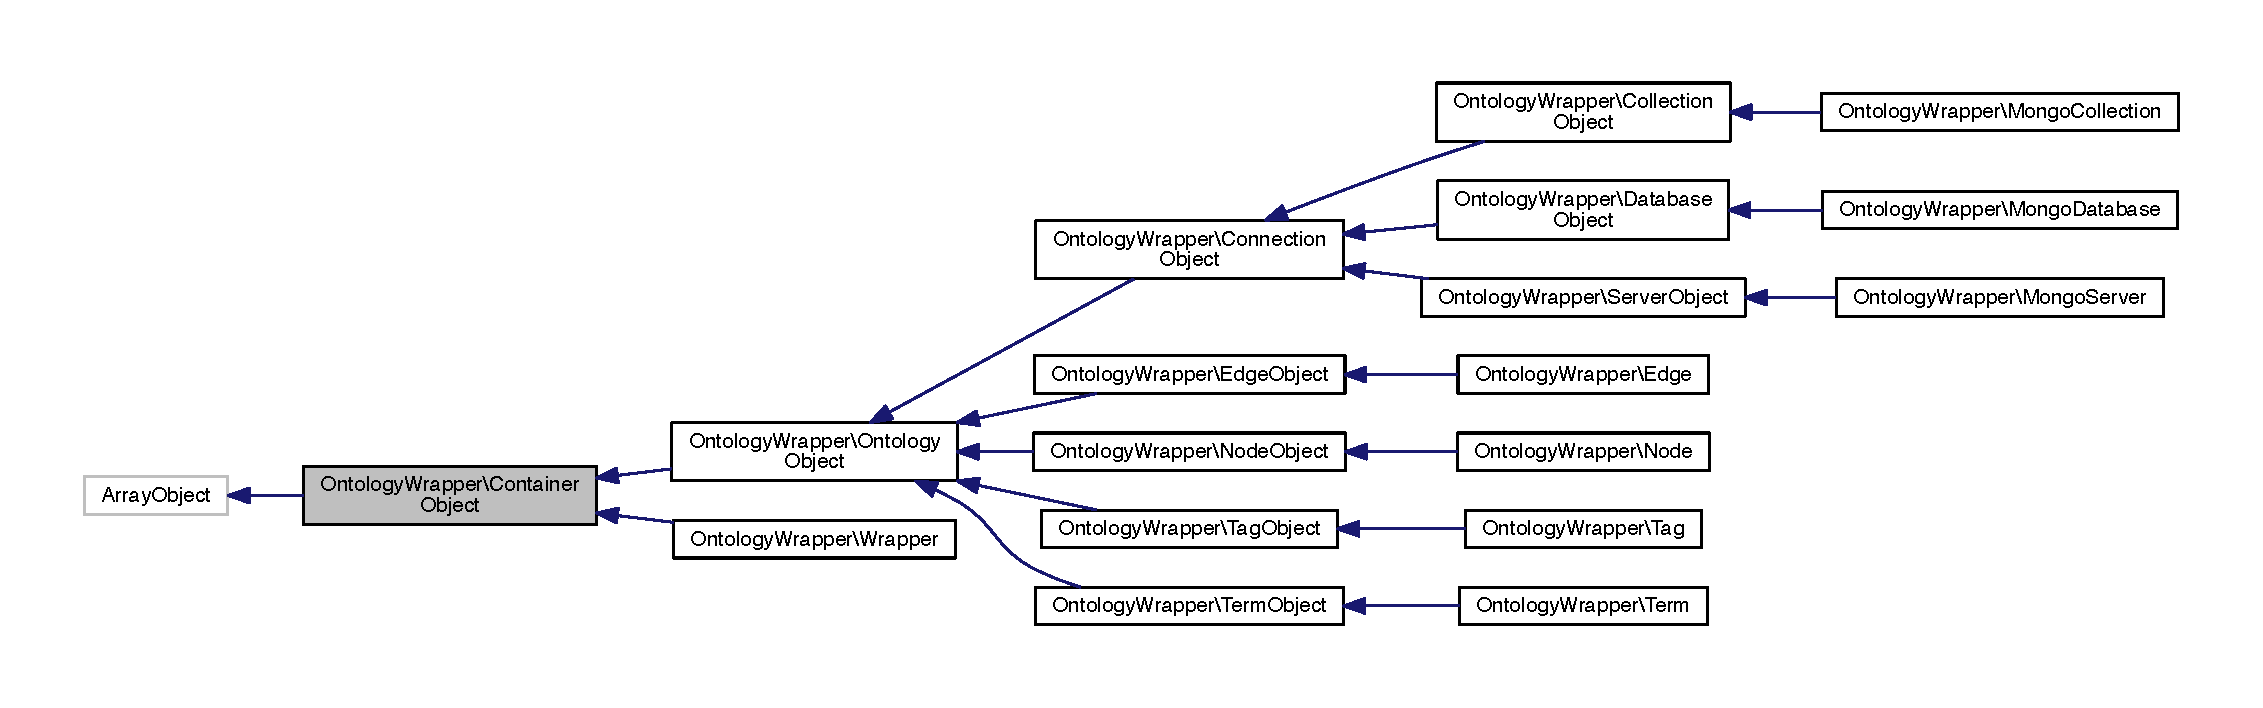
\includegraphics[width=350pt]{class_ontology_wrapper_1_1_container_object__inherit__graph}
\end{center}
\end{figure}


Collaboration diagram for Ontology\-Wrapper\textbackslash{}Container\-Object\-:
\nopagebreak
\begin{figure}[H]
\begin{center}
\leavevmode
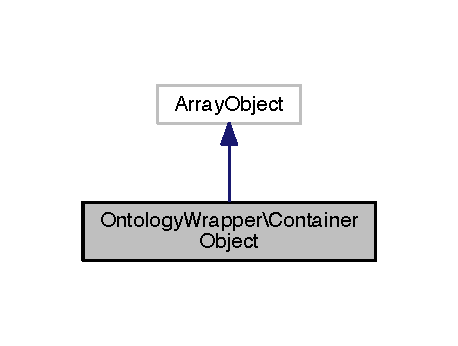
\includegraphics[width=220pt]{class_ontology_wrapper_1_1_container_object__coll__graph}
\end{center}
\end{figure}
\subsection*{Public Member Functions}
\begin{DoxyCompactItemize}
\item 
\hyperlink{class_ontology_wrapper_1_1_container_object_aff6fe69abda5124438458b687ab30c4f}{offset\-Exists} (\$the\-Offset)
\item 
\hyperlink{class_ontology_wrapper_1_1_container_object_a1fcd9bbec807c35973f634eb0a98ae13}{offset\-Get} (\$the\-Offset)
\item 
\hyperlink{class_ontology_wrapper_1_1_container_object_ae7c3dbc16f8e0e2bbd667c0168539a3e}{offset\-Set} (\$the\-Offset, \$the\-Value)
\item 
\hyperlink{class_ontology_wrapper_1_1_container_object_a6aec41ee5dafbd52a6e9963eb49f3e7e}{offset\-Unset} (\$the\-Offset)
\item 
\hyperlink{class_ontology_wrapper_1_1_container_object_ae27d07c2dcb4b4e95a167ef9fa6a419a}{array\-Keys} ()
\item 
\hyperlink{class_ontology_wrapper_1_1_container_object_a65780ec62aa8b6e5f699be556f9e316f}{array\-Values} ()
\end{DoxyCompactItemize}
\subsection*{Static Public Member Functions}
\begin{DoxyCompactItemize}
\item 
static \hyperlink{class_ontology_wrapper_1_1_container_object_a0af6d7a3fcaeeb50be636280e95bc2db}{Object2\-Array} (\&\$the\-Source, \&\$the\-Destination)
\end{DoxyCompactItemize}
\subsection*{Protected Member Functions}
\begin{DoxyCompactItemize}
\item 
\hyperlink{class_ontology_wrapper_1_1_container_object_ae03602f378081e220f8e6280d75bdc3e}{pre\-Offset\-Exists} (\&\$the\-Offset)
\item 
\hyperlink{class_ontology_wrapper_1_1_container_object_a7053dffd7fc10440eebfecd74e73d4af}{pre\-Offset\-Get} (\&\$the\-Offset)
\item 
\hyperlink{class_ontology_wrapper_1_1_container_object_ab7d07dda2c4b88ffa98b41d48814d03f}{pre\-Offset\-Set} (\&\$the\-Offset, \&\$the\-Value)
\item 
\hyperlink{class_ontology_wrapper_1_1_container_object_a0fa0ab4b7e742d00f2daa9206aa0b44a}{post\-Offset\-Set} (\&\$the\-Offset, \&\$the\-Value)
\item 
\hyperlink{class_ontology_wrapper_1_1_container_object_ae9f60cec5e7e40aed32c51dd7efa0429}{pre\-Offset\-Unset} (\&\$the\-Offset)
\item 
\hyperlink{class_ontology_wrapper_1_1_container_object_ada715084328ddac15b67491ea7c8e8cb}{post\-Offset\-Unset} (\&\$the\-Offset)
\item 
\hyperlink{class_ontology_wrapper_1_1_container_object_a9858b2ffc8e2c3474f1cc0f7a01df8d5}{manage\-Offset} (\$the\-Offset, \$the\-Value=N\-U\-L\-L, \$get\-Old=F\-A\-L\-S\-E)
\item 
\hyperlink{class_ontology_wrapper_1_1_container_object_a3fbfa8a211060c0407db32f31eba101b}{manage\-Set\-Offset} (\$the\-Offset, \$the\-Value, \$the\-Operation=N\-U\-L\-L, \$get\-Old=F\-A\-L\-S\-E)
\item 
\hyperlink{class_ontology_wrapper_1_1_container_object_aa0d380cae8b4eef94d7d9ba0098b1454}{manage\-Array\-Offset} (\$the\-Offset, \$the\-Key, \$the\-Value=N\-U\-L\-L, \$get\-Old=F\-A\-L\-S\-E)
\item 
\hyperlink{class_ontology_wrapper_1_1_container_object_ac54aca8b612d63b316350e8d9d82ebea}{manage\-Element\-Match\-Offset} (\$the\-Offset, \$the\-Type\-Offset, \$the\-Data\-Offset, \$the\-Type\-Value, \$the\-Data\-Value=N\-U\-L\-L, \$get\-Old=F\-A\-L\-S\-E)
\item 
\hyperlink{class_ontology_wrapper_1_1_container_object_afab5ff7dc87cde93bc899be69ffc7d21}{manage\-Property} (\&\$the\-Member, \$the\-Value=N\-U\-L\-L, \$get\-Old=F\-A\-L\-S\-E)
\end{DoxyCompactItemize}


\subsection{Detailed Description}
Container object

This class is the ancestor of classes that define objects that handle structured data and that are persistent.

The class extends {\ttfamily \hyperlink{}{Array\-Object}} by treating the inherited array as the persistent store and all other data members as run-\/time data. The convention is that items stored in the array part of the object are called {\itshape offsets} and are considered {\itshape persistent}, while all other data members are called {\itshape members} and are considered {\itshape run-\/time} data.

This class implements a framework that governs tha management of the object's persistent data. No offset may hold the {\ttfamily N\-U\-L\-L} value, setting an offset with {\ttfamily N\-U\-L\-L} value is equivalent to {\itshape deleting the offset}.

Retrieving non-\/existant offsets will {\itshape not} generate a warning, but only return {\ttfamily N\-U\-L\-L}.

The class features a series of methods that derived classes may use to customise the behaviour of the offset management methods\-:


\begin{DoxyItemize}
\item {\ttfamily \hyperlink{class_ontology_wrapper_1_1_container_object_ae03602f378081e220f8e6280d75bdc3e}{pre\-Offset\-Exists()}}\-: This method is called {\itshape before} the \hyperlink{class_ontology_wrapper_1_1_container_object_aff6fe69abda5124438458b687ab30c4f}{offset\-Exists()} method with the offset passed as a reference parameter, the method can be used to change the value of the offset or to provide a custom result\-: if the method returns {\ttfamily N\-U\-L\-L}, \hyperlink{class_ontology_wrapper_1_1_container_object_aff6fe69abda5124438458b687ab30c4f}{offset\-Exists()} will be called; if the method returns any other type of value, this will be returned and \hyperlink{class_ontology_wrapper_1_1_container_object_aff6fe69abda5124438458b687ab30c4f}{offset\-Exists()} will be skipped. 
\item {\ttfamily \hyperlink{class_ontology_wrapper_1_1_container_object_a7053dffd7fc10440eebfecd74e73d4af}{pre\-Offset\-Get()}}\-: This is called {\itshape before} the \hyperlink{class_ontology_wrapper_1_1_container_object_a1fcd9bbec807c35973f634eb0a98ae13}{offset\-Get()} method with the offset passed as a reference parameter, the method can be used to change the value of the offset or to provide a custom result\-: if the method returns {\ttfamily N\-U\-L\-L}, \hyperlink{class_ontology_wrapper_1_1_container_object_a1fcd9bbec807c35973f634eb0a98ae13}{offset\-Get()} will be called; if the method returns any other type of value, this will be returned and \hyperlink{class_ontology_wrapper_1_1_container_object_a1fcd9bbec807c35973f634eb0a98ae13}{offset\-Get()} will be skipped. 
\item {\ttfamily \hyperlink{class_ontology_wrapper_1_1_container_object_ab7d07dda2c4b88ffa98b41d48814d03f}{pre\-Offset\-Set()}}\-: This is called {\itshape before} the \hyperlink{class_ontology_wrapper_1_1_container_object_ae7c3dbc16f8e0e2bbd667c0168539a3e}{offset\-Set()} method with the offset and value passed as reference parameters, the method can be used to change the offset or the value\-: if the method returns {\ttfamily N\-U\-L\-L}, \hyperlink{class_ontology_wrapper_1_1_container_object_ae7c3dbc16f8e0e2bbd667c0168539a3e}{offset\-Set()} will be called; if the method returns any other type of value, the \hyperlink{class_ontology_wrapper_1_1_container_object_ae7c3dbc16f8e0e2bbd667c0168539a3e}{offset\-Set()} will be skipped. 
\item {\ttfamily \hyperlink{class_ontology_wrapper_1_1_container_object_a0fa0ab4b7e742d00f2daa9206aa0b44a}{post\-Offset\-Set()}}\-: This is called {\itshape after} the \hyperlink{class_ontology_wrapper_1_1_container_object_ae7c3dbc16f8e0e2bbd667c0168539a3e}{offset\-Set()} method with the offset and value passed as reference parameters, the method can be used to set status or statistical variables, it will only be called if the \hyperlink{class_ontology_wrapper_1_1_container_object_ae7c3dbc16f8e0e2bbd667c0168539a3e}{offset\-Set()} method was called. 
\item {\ttfamily \hyperlink{class_ontology_wrapper_1_1_container_object_ae9f60cec5e7e40aed32c51dd7efa0429}{pre\-Offset\-Unset()}}\-: This is called {\itshape before} the \hyperlink{class_ontology_wrapper_1_1_container_object_a6aec41ee5dafbd52a6e9963eb49f3e7e}{offset\-Unset()} method with the offset passed as a reference parameter, the method can be used to change the offset\-: if the method returns {\ttfamily N\-U\-L\-L}, \hyperlink{class_ontology_wrapper_1_1_container_object_a6aec41ee5dafbd52a6e9963eb49f3e7e}{offset\-Unset()} will be called; if the method returns any other type of value, the \hyperlink{class_ontology_wrapper_1_1_container_object_a6aec41ee5dafbd52a6e9963eb49f3e7e}{offset\-Unset()} will be skipped. 
\item {\ttfamily \hyperlink{class_ontology_wrapper_1_1_container_object_ada715084328ddac15b67491ea7c8e8cb}{post\-Offset\-Unset()}}\-: This is called {\itshape after} the \hyperlink{class_ontology_wrapper_1_1_container_object_a6aec41ee5dafbd52a6e9963eb49f3e7e}{offset\-Unset()} method with the offset passed as a reference parameter, the method can be used to set status or statistical variables, it will only be called if the \hyperlink{class_ontology_wrapper_1_1_container_object_a6aec41ee5dafbd52a6e9963eb49f3e7e}{offset\-Unset()} method was called. 
\end{DoxyItemize}

The class features a series of methods that are useful for handling the persistent data as a whole\-:


\begin{DoxyItemize}
\item {\itshape \hyperlink{class_ontology_wrapper_1_1_container_object_ae27d07c2dcb4b4e95a167ef9fa6a419a}{array\-Keys()}}\-: This method is the equivalent of the \hyperlink{}{array\-\_\-keys()} function. 
\item {\itshape \hyperlink{class_ontology_wrapper_1_1_container_object_a65780ec62aa8b6e5f699be556f9e316f}{array\-Values()}}\-: This method is the equivalent of the \hyperlink{}{array\-\_\-values()} function. 
\end{DoxyItemize}

The class features a static method, \hyperlink{class_ontology_wrapper_1_1_container_object_a0af6d7a3fcaeeb50be636280e95bc2db}{Object2\-Array}, that can be used to convert a structure of nested \hyperlink{}{Array\-Object} instances into a nested array, this will be useful when normalising objects before persisting.

This class implements a series of methods that can be used by member accessor methods to handle properties and offsets in a standard way\-:


\begin{DoxyItemize}
\item {\itshape \hyperlink{class_ontology_wrapper_1_1_container_object_a9858b2ffc8e2c3474f1cc0f7a01df8d5}{manage\-Offset()}}\-: This method provides a standard interface to set, retrieve and delete offset values. 
\item {\itshape \hyperlink{class_ontology_wrapper_1_1_container_object_a3fbfa8a211060c0407db32f31eba101b}{manage\-Set\-Offset()}}\-: This method provides a standard interface to set, retrieve and delete elements of an array set, this method provides access to elements of the offset, rather than to the offset, which must be an array or \hyperlink{}{Array\-Object}. 
\item {\itshape \hyperlink{class_ontology_wrapper_1_1_container_object_ac54aca8b612d63b316350e8d9d82ebea}{manage\-Element\-Match\-Offset()}}\-: This method provides a standard interface to set, retrieve and delete elements of an array or \hyperlink{}{Array\-Object}, these elements are an array of two items in which the first one is the discriminator and the second is the value. 
\item {\itshape \hyperlink{class_ontology_wrapper_1_1_container_object_afab5ff7dc87cde93bc899be69ffc7d21}{manage\-Property()}}\-: This method provides a standard interface to set, retrieve and reset data members. 
\end{DoxyItemize}\begin{DoxyVerb} @author            Milko A. Škofič <m.skofic@cgiar.org>
 @version   1.00 10/01/2014\end{DoxyVerb}
 

\subsection{Member Function Documentation}
\hypertarget{class_ontology_wrapper_1_1_container_object_ae27d07c2dcb4b4e95a167ef9fa6a419a}{\index{Ontology\-Wrapper\-::\-Container\-Object@{Ontology\-Wrapper\-::\-Container\-Object}!array\-Keys@{array\-Keys}}
\index{array\-Keys@{array\-Keys}!OntologyWrapper::ContainerObject@{Ontology\-Wrapper\-::\-Container\-Object}}
\subsubsection[{array\-Keys}]{\setlength{\rightskip}{0pt plus 5cm}Ontology\-Wrapper\textbackslash{}\-Container\-Object\-::array\-Keys (
\begin{DoxyParamCaption}
{}
\end{DoxyParamCaption}
)}}\label{class_ontology_wrapper_1_1_container_object_ae27d07c2dcb4b4e95a167ef9fa6a419a}
Return object's offsets

This method has the same function as the P\-H\-P function \hyperlink{}{array\-\_\-keys()}, it will return all the object's offset keys as an array.

public \begin{DoxyReturn}{Returns}
array List of object offsets.
\end{DoxyReturn}
get\-Array\-Copy() \hypertarget{class_ontology_wrapper_1_1_container_object_a65780ec62aa8b6e5f699be556f9e316f}{\index{Ontology\-Wrapper\-::\-Container\-Object@{Ontology\-Wrapper\-::\-Container\-Object}!array\-Values@{array\-Values}}
\index{array\-Values@{array\-Values}!OntologyWrapper::ContainerObject@{Ontology\-Wrapper\-::\-Container\-Object}}
\subsubsection[{array\-Values}]{\setlength{\rightskip}{0pt plus 5cm}Ontology\-Wrapper\textbackslash{}\-Container\-Object\-::array\-Values (
\begin{DoxyParamCaption}
{}
\end{DoxyParamCaption}
)}}\label{class_ontology_wrapper_1_1_container_object_a65780ec62aa8b6e5f699be556f9e316f}
Return object's offset values

This method has the same function as the P\-H\-P function \hyperlink{}{array\-\_\-values()}, it will return all the object's offset values as an array.

public \begin{DoxyReturn}{Returns}
array List of object offset values.
\end{DoxyReturn}
get\-Array\-Copy() \hypertarget{class_ontology_wrapper_1_1_container_object_aa0d380cae8b4eef94d7d9ba0098b1454}{\index{Ontology\-Wrapper\-::\-Container\-Object@{Ontology\-Wrapper\-::\-Container\-Object}!manage\-Array\-Offset@{manage\-Array\-Offset}}
\index{manage\-Array\-Offset@{manage\-Array\-Offset}!OntologyWrapper::ContainerObject@{Ontology\-Wrapper\-::\-Container\-Object}}
\subsubsection[{manage\-Array\-Offset}]{\setlength{\rightskip}{0pt plus 5cm}Ontology\-Wrapper\textbackslash{}\-Container\-Object\-::manage\-Array\-Offset (
\begin{DoxyParamCaption}
\item[{}]{\$the\-Offset, }
\item[{}]{\$the\-Key, }
\item[{}]{\$the\-Value = {\ttfamily NULL}, }
\item[{}]{\$get\-Old = {\ttfamily FALSE}}
\end{DoxyParamCaption}
)\hspace{0.3cm}{\ttfamily [protected]}}}\label{class_ontology_wrapper_1_1_container_object_aa0d380cae8b4eef94d7d9ba0098b1454}
\subparagraph*{Manage value set offset}

This class provides a protected interface for member accessor methods, both for properties and offsets, this method can be used to manage the elements of a key/value array, its options involve setting, retrieving and deleting elements of the list by key. This method generally applies to data of the \hyperlink{}{k\-T\-Y\-P\-E\-\_\-\-A\-R\-R\-A\-Y} data type.

It is assumed that the value at the provided offset is either an array or an \hyperlink{}{Array\-Object}, if this is not the case, the method will raise an exception.

If you want to manage the array itself, you have to use the offset management
\begin{DoxyItemize}
\item methods.

The method accepts the following parameters\-:


\begin{DoxyItemize}
\item {\ttfamily \$the\-Offset}\-: The offset to the array attribute that is to be managed. 
\item {\ttfamily \$the\-Key}\-: The element key. 
\item {\ttfamily \$the\-Value}\-: The element value or operation\-: 
\begin{DoxyItemize}
\item {\ttfamily N\-U\-L\-L}\-: Return the value at the provided key, or {\ttfamily N\-U\-L\-L}. 
\item {\ttfamily F\-A\-L\-S\-E}\-: Delete the value at the provided key. 
\item {\itshape other}\-: Any other type represents a new or a replacement value. 
\end{DoxyItemize}
\item {\ttfamily \$get\-Old}\-: Determines what the method will return\-: 
\begin{DoxyItemize}
\item {\ttfamily T\-R\-U\-E}\-: Return the value {\itshape before} it was eventually modified. 
\item {\ttfamily F\-A\-L\-S\-E}\-: Return the value {\itshape after} it was eventually modified. 
\end{DoxyItemize}
\end{DoxyItemize}

When setting new values, if the current offset is empty, the method will set the new value in an aray; when deleting values, if the existing value is the last one, the method will delete the offset itself.


\begin{DoxyParams}[1]{Parameters}
string & {\em \$the\-Offset} & Offset to be managed. \\
\hline
mixed & {\em \$the\-Key} & Element key. \\
\hline
mixed & {\em \$the\-Value} & Element value or operation. \\
\hline
boolean & {\em \$get\-Old} & T\-R\-U\-E get old value.\\
\hline
\end{DoxyParams}
protected \begin{DoxyReturn}{Returns}
mixed Old or new value.
\end{DoxyReturn}

\begin{DoxyExceptions}{Exceptions}
{\em Exception} & \hyperlink{class_ontology_wrapper_1_1_container_object_ae7c3dbc16f8e0e2bbd667c0168539a3e}{offset\-Set()}  \hyperlink{class_ontology_wrapper_1_1_container_object_a1fcd9bbec807c35973f634eb0a98ae13}{offset\-Get()}  \hyperlink{class_ontology_wrapper_1_1_container_object_a6aec41ee5dafbd52a6e9963eb49f3e7e}{offset\-Unset()} \\
\hline
\end{DoxyExceptions}

\end{DoxyItemize}\hypertarget{class_ontology_wrapper_1_1_container_object_ac54aca8b612d63b316350e8d9d82ebea}{\index{Ontology\-Wrapper\-::\-Container\-Object@{Ontology\-Wrapper\-::\-Container\-Object}!manage\-Element\-Match\-Offset@{manage\-Element\-Match\-Offset}}
\index{manage\-Element\-Match\-Offset@{manage\-Element\-Match\-Offset}!OntologyWrapper::ContainerObject@{Ontology\-Wrapper\-::\-Container\-Object}}
\subsubsection[{manage\-Element\-Match\-Offset}]{\setlength{\rightskip}{0pt plus 5cm}Ontology\-Wrapper\textbackslash{}\-Container\-Object\-::manage\-Element\-Match\-Offset (
\begin{DoxyParamCaption}
\item[{}]{\$the\-Offset, }
\item[{}]{\$the\-Type\-Offset, }
\item[{}]{\$the\-Data\-Offset, }
\item[{}]{\$the\-Type\-Value, }
\item[{}]{\$the\-Data\-Value = {\ttfamily NULL}, }
\item[{}]{\$get\-Old = {\ttfamily FALSE}}
\end{DoxyParamCaption}
)\hspace{0.3cm}{\ttfamily [protected]}}}\label{class_ontology_wrapper_1_1_container_object_ac54aca8b612d63b316350e8d9d82ebea}
\subparagraph*{Manage element match offset}

This class provides a protected interface for member accessor methods, both for properties and offsets, this method can be used to manage the elements of an array of array elements in which one item's value represents the discriminant.

Offsets of this kind are arrays or \hyperlink{}{Array\-Object} instances that represent a list of elements, each of which is constituted by an array of two elements, where the value matching the {\ttfamily \$the\-Type\-Offset} key represents the element key and the value matching the {\ttfamily \$the\-Data\-Offset} key represents the element's value.

This method allows retrieving the element value and deleting or setting an element.

It is assumed that the value at the provided offset is either an array or an \hyperlink{}{Array\-Object}, if this is not the case, the method will raise an exception.

If you want to manage the set itself, you have to use the offset management methods.

The method accepts the following parameters\-:


\begin{DoxyItemize}
\item {\ttfamily \$the\-Offset}\-: The offset to the attribute containing the match list. 
\item {\ttfamily \$the\-Type\-Offset}\-: The offset to the type within the element. 
\item {\ttfamily \$the\-Data\-Offset}\-: The offset to the data within the element. 
\item {\ttfamily \$the\-Type\-Value}\-: The value of the element's type to match, it represents the key to the element; we assume the value to be a string. A {\ttfamily N\-U\-L\-L} value is used to select the element missing the {\ttfamily \$the\-Type\-Offset} offset. 
\item {\ttfamily \$the\-Data\-Value}\-: The value or operation\-: 
\begin{DoxyItemize}
\item {\ttfamily N\-U\-L\-L}\-: Return the offset's {\ttfamily \$the\-Data\-Offset} value. 
\item {\ttfamily F\-A\-L\-S\-E}\-: Delete the element matchhing the {\ttfamily \$the\-Type\-Offset}. 
\item {\itshape other}\-: Any other type represents the element's new value. 
\end{DoxyItemize}
\item {\ttfamily \$get\-Old}\-: Determines what the method will return\-: 
\begin{DoxyItemize}
\item {\ttfamily T\-R\-U\-E}\-: Return the value of the offset {\itshape before} it was eventually modified. 
\item {\ttfamily F\-A\-L\-S\-E}\-: Return the value of the offset {\itshape after} it was eventually modified. 
\end{DoxyItemize}
\end{DoxyItemize}

The method expects each element to be a structure containing at least an element indexed by the {\ttfamily \$the\-Data\-Offset} offset, if that is not the case, the method will raise an exception. All elements are supposed to be arrays.


\begin{DoxyParams}[1]{Parameters}
string & {\em \$the\-Offset} & Offset to be managed. \\
\hline
string & {\em \$the\-Type\-Offset} & Offset of type item. \\
\hline
string & {\em \$the\-Data\-Offset} & Offset of data item. \\
\hline
string & {\em \$the\-Type\-Value} & Type value. \\
\hline
mixed & {\em \$the\-Data\-Value} & New value or operation. \\
\hline
boolean & {\em \$get\-Old} & T\-R\-U\-E get old value.\\
\hline
\end{DoxyParams}
protected \begin{DoxyReturn}{Returns}
mixed Old or new value.
\end{DoxyReturn}

\begin{DoxyExceptions}{Exceptions}
{\em Exception} & \hyperlink{class_ontology_wrapper_1_1_container_object_ae7c3dbc16f8e0e2bbd667c0168539a3e}{offset\-Set()}  \hyperlink{class_ontology_wrapper_1_1_container_object_a1fcd9bbec807c35973f634eb0a98ae13}{offset\-Get()}  \hyperlink{class_ontology_wrapper_1_1_container_object_a6aec41ee5dafbd52a6e9963eb49f3e7e}{offset\-Unset()} \\
\hline
\end{DoxyExceptions}
\hypertarget{class_ontology_wrapper_1_1_container_object_a9858b2ffc8e2c3474f1cc0f7a01df8d5}{\index{Ontology\-Wrapper\-::\-Container\-Object@{Ontology\-Wrapper\-::\-Container\-Object}!manage\-Offset@{manage\-Offset}}
\index{manage\-Offset@{manage\-Offset}!OntologyWrapper::ContainerObject@{Ontology\-Wrapper\-::\-Container\-Object}}
\subsubsection[{manage\-Offset}]{\setlength{\rightskip}{0pt plus 5cm}Ontology\-Wrapper\textbackslash{}\-Container\-Object\-::manage\-Offset (
\begin{DoxyParamCaption}
\item[{}]{\$the\-Offset, }
\item[{}]{\$the\-Value = {\ttfamily NULL}, }
\item[{}]{\$get\-Old = {\ttfamily FALSE}}
\end{DoxyParamCaption}
)\hspace{0.3cm}{\ttfamily [protected]}}}\label{class_ontology_wrapper_1_1_container_object_a9858b2ffc8e2c3474f1cc0f7a01df8d5}
\subparagraph*{Manage a scalar offset}

This class provides a protected interface for member accessor methods, both for properties and offsets, this method can be used to manage a scalar offset, its options involve setting, retrieving and deleting an offset of the provided array or Array\-Object.

The method accepts the following parameters\-:


\begin{DoxyItemize}
\item {\ttfamily \$the\-Offset}\-: The offset to the attribute contained in the previous parameter that is to be managed. 
\item {\ttfamily \$the\-Value}\-: The value or operation\-: 
\begin{DoxyItemize}
\item {\ttfamily N\-U\-L\-L}\-: Return the offset's current value. 
\item {\ttfamily F\-A\-L\-S\-E}\-: Delete the offset. 
\item {\itshape other}\-: Any other type represents the offset's new value. 
\end{DoxyItemize}
\item {\ttfamily \$get\-Old}\-: Determines what the method will return\-: 
\begin{DoxyItemize}
\item {\ttfamily T\-R\-U\-E}\-: Return the value of the offset {\itshape before} it was eventually modified. 
\item {\ttfamily F\-A\-L\-S\-E}\-: Return the value of the offset {\itshape after} it was eventually modified. 
\end{DoxyItemize}
\end{DoxyItemize}


\begin{DoxyParams}[1]{Parameters}
string & {\em \$the\-Offset} & Offset to be managed. \\
\hline
mixed & {\em \$the\-Value} & New value or operation. \\
\hline
boolean & {\em \$get\-Old} & T\-R\-U\-E get old value.\\
\hline
\end{DoxyParams}
protected \begin{DoxyReturn}{Returns}
mixed Old or new value.
\end{DoxyReturn}
\hyperlink{class_ontology_wrapper_1_1_container_object_ae7c3dbc16f8e0e2bbd667c0168539a3e}{offset\-Set()}  \hyperlink{class_ontology_wrapper_1_1_container_object_a1fcd9bbec807c35973f634eb0a98ae13}{offset\-Get()}  \hyperlink{class_ontology_wrapper_1_1_container_object_a6aec41ee5dafbd52a6e9963eb49f3e7e}{offset\-Unset()} \hypertarget{class_ontology_wrapper_1_1_container_object_afab5ff7dc87cde93bc899be69ffc7d21}{\index{Ontology\-Wrapper\-::\-Container\-Object@{Ontology\-Wrapper\-::\-Container\-Object}!manage\-Property@{manage\-Property}}
\index{manage\-Property@{manage\-Property}!OntologyWrapper::ContainerObject@{Ontology\-Wrapper\-::\-Container\-Object}}
\subsubsection[{manage\-Property}]{\setlength{\rightskip}{0pt plus 5cm}Ontology\-Wrapper\textbackslash{}\-Container\-Object\-::manage\-Property (
\begin{DoxyParamCaption}
\item[{\&}]{\$the\-Member, }
\item[{}]{\$the\-Value = {\ttfamily NULL}, }
\item[{}]{\$get\-Old = {\ttfamily FALSE}}
\end{DoxyParamCaption}
)\hspace{0.3cm}{\ttfamily [protected]}}}\label{class_ontology_wrapper_1_1_container_object_afab5ff7dc87cde93bc899be69ffc7d21}
\subparagraph*{Manage a property}

This library implements a standard interface for managing object properties using accessor methods, this method implements this interface\-:


\begin{DoxyItemize}
\item {\ttfamily \&\$the\-Member}\-: Reference to the property being managed. 
\item {\ttfamily \$the\-Value}\-: The property value or operation\-: 
\begin{DoxyItemize}
\item {\ttfamily N\-U\-L\-L}\-: Return the current property value. 
\item {\ttfamily F\-A\-L\-S\-E}\-: Reset the property to {\ttfamily N\-U\-L\-L}, the default value. 
\item {\itshape other}\-: Any other type represents the new value of the property. 
\end{DoxyItemize}
\item {\ttfamily \$get\-Old}\-: Determines what the method will return\-: 
\begin{DoxyItemize}
\item {\ttfamily T\-R\-U\-E}\-: Return the value of the property {\itshape before} it was eventually modified. 
\item {\ttfamily F\-A\-L\-S\-E}\-: Return the value of the property {\itshape after} it was eventually modified. 
\end{DoxyItemize}
\end{DoxyItemize}


\begin{DoxyParams}[1]{Parameters}
reference & {\em \$the\-Member} & Reference to the data member. \\
\hline
mixed & {\em \$the\-Value} & Value or operation. \\
\hline
boolean & {\em \$get\-Old} & {\ttfamily T\-R\-U\-E} get old value.\\
\hline
\end{DoxyParams}
protected \begin{DoxyReturn}{Returns}
mixed Old or new property value. 
\end{DoxyReturn}
\hypertarget{class_ontology_wrapper_1_1_container_object_a3fbfa8a211060c0407db32f31eba101b}{\index{Ontology\-Wrapper\-::\-Container\-Object@{Ontology\-Wrapper\-::\-Container\-Object}!manage\-Set\-Offset@{manage\-Set\-Offset}}
\index{manage\-Set\-Offset@{manage\-Set\-Offset}!OntologyWrapper::ContainerObject@{Ontology\-Wrapper\-::\-Container\-Object}}
\subsubsection[{manage\-Set\-Offset}]{\setlength{\rightskip}{0pt plus 5cm}Ontology\-Wrapper\textbackslash{}\-Container\-Object\-::manage\-Set\-Offset (
\begin{DoxyParamCaption}
\item[{}]{\$the\-Offset, }
\item[{}]{\$the\-Value, }
\item[{}]{\$the\-Operation = {\ttfamily NULL}, }
\item[{}]{\$get\-Old = {\ttfamily FALSE}}
\end{DoxyParamCaption}
)\hspace{0.3cm}{\ttfamily [protected]}}}\label{class_ontology_wrapper_1_1_container_object_a3fbfa8a211060c0407db32f31eba101b}
\subparagraph*{Manage value set offset}

This class provides a protected interface for member accessor methods, both for properties and offsets, this method can be used to manage the elements of a set of non repeting values, its options involve setting, retrieving and deleting elements of the set. This method generally applies to data of the \hyperlink{}{k\-T\-Y\-P\-E\-\_\-\-S\-E\-T} data type.

It is assumed that the value at the provided offset is either an array or an \hyperlink{}{Array\-Object}, if this is not the case, the method will raise an exception.

If you want to manage the set itself, you have to use the offset management methods.

The method accepts the following parameters\-:


\begin{DoxyItemize}
\item {\ttfamily \$the\-Offset}\-: The offset to the array attribute that is to be managed. 
\item {\ttfamily \$the\-Value}\-: The value of the array element. 
\item {\ttfamily \$the\-Operation}\-: The operation\-: 
\begin{DoxyItemize}
\item {\ttfamily N\-U\-L\-L}\-: Return the value if it exists or {\ttfamily N\-U\-L\-L}. 
\item {\ttfamily F\-A\-L\-S\-E}\-: Delete the value if it exists. 
\item {\itshape other}\-: Any other type represents a new value. 
\end{DoxyItemize}
\item {\ttfamily \$get\-Old}\-: Determines what the method will return\-: 
\begin{DoxyItemize}
\item {\ttfamily T\-R\-U\-E}\-: Return the value {\itshape before} it was eventually modified. 
\item {\ttfamily F\-A\-L\-S\-E}\-: Return the value {\itshape after} it was eventually modified. 
\end{DoxyItemize}
\end{DoxyItemize}

When setting new values, if the current offset is empty, the method will set the new value in an aray; when deleting values, if the existing value is the last one, the method will delete the offset itself.


\begin{DoxyParams}[1]{Parameters}
string & {\em \$the\-Offset} & Offset to be managed. \\
\hline
mixed & {\em \$the\-Value} & Array value. \\
\hline
mixed & {\em \$the\-Operation} & Operation. \\
\hline
boolean & {\em \$get\-Old} & T\-R\-U\-E get old value.\\
\hline
\end{DoxyParams}
protected \begin{DoxyReturn}{Returns}
mixed Old or new value.
\end{DoxyReturn}

\begin{DoxyExceptions}{Exceptions}
{\em Exception} & \hyperlink{class_ontology_wrapper_1_1_container_object_ae7c3dbc16f8e0e2bbd667c0168539a3e}{offset\-Set()}  \hyperlink{class_ontology_wrapper_1_1_container_object_a1fcd9bbec807c35973f634eb0a98ae13}{offset\-Get()}  \hyperlink{class_ontology_wrapper_1_1_container_object_a6aec41ee5dafbd52a6e9963eb49f3e7e}{offset\-Unset()} \\
\hline
\end{DoxyExceptions}
\hypertarget{class_ontology_wrapper_1_1_container_object_a0af6d7a3fcaeeb50be636280e95bc2db}{\index{Ontology\-Wrapper\-::\-Container\-Object@{Ontology\-Wrapper\-::\-Container\-Object}!Object2\-Array@{Object2\-Array}}
\index{Object2\-Array@{Object2\-Array}!OntologyWrapper::ContainerObject@{Ontology\-Wrapper\-::\-Container\-Object}}
\subsubsection[{Object2\-Array}]{\setlength{\rightskip}{0pt plus 5cm}static Ontology\-Wrapper\textbackslash{}\-Container\-Object\-::\-Object2\-Array (
\begin{DoxyParamCaption}
\item[{\&}]{\$the\-Source, }
\item[{\&}]{\$the\-Destination}
\end{DoxyParamCaption}
)\hspace{0.3cm}{\ttfamily [static]}}}\label{class_ontology_wrapper_1_1_container_object_a0af6d7a3fcaeeb50be636280e95bc2db}
\subparagraph*{Convert object to array}

This method can be used to obtain an array of arrays from a nested structure.

The method expects as the first parameter a reference to an \hyperlink{}{Array\-Object} or to an array, it will convert the provided parameter to an array and traverse it, converting recursively any \hyperlink{}{Array\-Object} instance into an array.

The method accepts the following parameters\-:


\begin{DoxyItemize}
\item {\ttfamily \$the\-Source}\-: Source structure reference ({\itshape read-\/only}). 
\item {\ttfamily \$the\-Destination}\-: Destination array reference. 
\end{DoxyItemize}


\begin{DoxyParams}[1]{Parameters}
reference & {\em \$the\-Source} & Reference to the source structure. \\
\hline
reference & {\em \$the\-Destination} & Reference to the destination array.\\
\hline
\end{DoxyParams}

\begin{DoxyExceptions}{Exceptions}
{\em Exception} & \\
\hline
\end{DoxyExceptions}
\hypertarget{class_ontology_wrapper_1_1_container_object_aff6fe69abda5124438458b687ab30c4f}{\index{Ontology\-Wrapper\-::\-Container\-Object@{Ontology\-Wrapper\-::\-Container\-Object}!offset\-Exists@{offset\-Exists}}
\index{offset\-Exists@{offset\-Exists}!OntologyWrapper::ContainerObject@{Ontology\-Wrapper\-::\-Container\-Object}}
\subsubsection[{offset\-Exists}]{\setlength{\rightskip}{0pt plus 5cm}Ontology\-Wrapper\textbackslash{}\-Container\-Object\-::offset\-Exists (
\begin{DoxyParamCaption}
\item[{}]{\$the\-Offset}
\end{DoxyParamCaption}
)}}\label{class_ontology_wrapper_1_1_container_object_aff6fe69abda5124438458b687ab30c4f}
Check if an offset exists

We overload this method to call the preflight method\-: if it returns {\ttfamily N\-U\-L\-L} we call the parent method; if not, we return the received value.


\begin{DoxyParams}[1]{Parameters}
mixed & {\em \$the\-Offset} & Offset.\\
\hline
\end{DoxyParams}
public \begin{DoxyReturn}{Returns}
boolean {\ttfamily T\-R\-U\-E} the offset exists.
\end{DoxyReturn}
\hyperlink{class_ontology_wrapper_1_1_container_object_ae03602f378081e220f8e6280d75bdc3e}{pre\-Offset\-Exists()} \hypertarget{class_ontology_wrapper_1_1_container_object_a1fcd9bbec807c35973f634eb0a98ae13}{\index{Ontology\-Wrapper\-::\-Container\-Object@{Ontology\-Wrapper\-::\-Container\-Object}!offset\-Get@{offset\-Get}}
\index{offset\-Get@{offset\-Get}!OntologyWrapper::ContainerObject@{Ontology\-Wrapper\-::\-Container\-Object}}
\subsubsection[{offset\-Get}]{\setlength{\rightskip}{0pt plus 5cm}Ontology\-Wrapper\textbackslash{}\-Container\-Object\-::offset\-Get (
\begin{DoxyParamCaption}
\item[{}]{\$the\-Offset}
\end{DoxyParamCaption}
)}}\label{class_ontology_wrapper_1_1_container_object_a1fcd9bbec807c35973f634eb0a98ae13}
Return a value at a given offset

We overload this method to call the preflight method\-: if it returns {\ttfamily N\-U\-L\-L} we call the parent method; if not, we return the received value.

We also overload this method to handle unmatched offsets\-: we prevent warnings from being issued and return {\ttfamily N\-U\-L\-L}.


\begin{DoxyParams}[1]{Parameters}
mixed & {\em \$the\-Offset} & Offset.\\
\hline
\end{DoxyParams}
public \begin{DoxyReturn}{Returns}
mixed Offset value or {\ttfamily N\-U\-L\-L}.
\end{DoxyReturn}
\hyperlink{class_ontology_wrapper_1_1_container_object_a7053dffd7fc10440eebfecd74e73d4af}{pre\-Offset\-Get()} \hypertarget{class_ontology_wrapper_1_1_container_object_ae7c3dbc16f8e0e2bbd667c0168539a3e}{\index{Ontology\-Wrapper\-::\-Container\-Object@{Ontology\-Wrapper\-::\-Container\-Object}!offset\-Set@{offset\-Set}}
\index{offset\-Set@{offset\-Set}!OntologyWrapper::ContainerObject@{Ontology\-Wrapper\-::\-Container\-Object}}
\subsubsection[{offset\-Set}]{\setlength{\rightskip}{0pt plus 5cm}Ontology\-Wrapper\textbackslash{}\-Container\-Object\-::offset\-Set (
\begin{DoxyParamCaption}
\item[{}]{\$the\-Offset, }
\item[{}]{\$the\-Value}
\end{DoxyParamCaption}
)}}\label{class_ontology_wrapper_1_1_container_object_ae7c3dbc16f8e0e2bbd667c0168539a3e}
Set a value at a given offset

We overload this method to call the preflight and postflight methods\-: if the preflight method returns {\ttfamily N\-U\-L\-L} we call the parent method; if not, we stop.

We also overload this method to handle {\ttfamily N\-U\-L\-L} {\itshape values}\-: in that case we delete the offset.


\begin{DoxyParams}[1]{Parameters}
string & {\em \$the\-Offset} & Offset. \\
\hline
mixed & {\em \$the\-Value} & Value to set at offset.\\
\hline
\end{DoxyParams}
public

\hyperlink{class_ontology_wrapper_1_1_container_object_ab7d07dda2c4b88ffa98b41d48814d03f}{pre\-Offset\-Set()}  \hyperlink{class_ontology_wrapper_1_1_container_object_a0fa0ab4b7e742d00f2daa9206aa0b44a}{post\-Offset\-Set()}  \hyperlink{class_ontology_wrapper_1_1_container_object_a6aec41ee5dafbd52a6e9963eb49f3e7e}{offset\-Unset()} \hypertarget{class_ontology_wrapper_1_1_container_object_a6aec41ee5dafbd52a6e9963eb49f3e7e}{\index{Ontology\-Wrapper\-::\-Container\-Object@{Ontology\-Wrapper\-::\-Container\-Object}!offset\-Unset@{offset\-Unset}}
\index{offset\-Unset@{offset\-Unset}!OntologyWrapper::ContainerObject@{Ontology\-Wrapper\-::\-Container\-Object}}
\subsubsection[{offset\-Unset}]{\setlength{\rightskip}{0pt plus 5cm}Ontology\-Wrapper\textbackslash{}\-Container\-Object\-::offset\-Unset (
\begin{DoxyParamCaption}
\item[{}]{\$the\-Offset}
\end{DoxyParamCaption}
)}}\label{class_ontology_wrapper_1_1_container_object_a6aec41ee5dafbd52a6e9963eb49f3e7e}
Reset a value at a given offset

We overload this method to call the preflight and postflight methods\-: if the preflight method returns {\ttfamily N\-U\-L\-L} we call the parent method; if not, we stop.

We also overload this method to prevent warnings on unmatched offsets.


\begin{DoxyParams}[1]{Parameters}
string & {\em \$the\-Offset} & Offset.\\
\hline
\end{DoxyParams}
public

\hyperlink{class_ontology_wrapper_1_1_container_object_ae9f60cec5e7e40aed32c51dd7efa0429}{pre\-Offset\-Unset()}  \hyperlink{class_ontology_wrapper_1_1_container_object_ada715084328ddac15b67491ea7c8e8cb}{post\-Offset\-Unset()} \hypertarget{class_ontology_wrapper_1_1_container_object_a0fa0ab4b7e742d00f2daa9206aa0b44a}{\index{Ontology\-Wrapper\-::\-Container\-Object@{Ontology\-Wrapper\-::\-Container\-Object}!post\-Offset\-Set@{post\-Offset\-Set}}
\index{post\-Offset\-Set@{post\-Offset\-Set}!OntologyWrapper::ContainerObject@{Ontology\-Wrapper\-::\-Container\-Object}}
\subsubsection[{post\-Offset\-Set}]{\setlength{\rightskip}{0pt plus 5cm}Ontology\-Wrapper\textbackslash{}\-Container\-Object\-::post\-Offset\-Set (
\begin{DoxyParamCaption}
\item[{\&}]{\$the\-Offset, }
\item[{\&}]{\$the\-Value}
\end{DoxyParamCaption}
)\hspace{0.3cm}{\ttfamily [protected]}}}\label{class_ontology_wrapper_1_1_container_object_a0fa0ab4b7e742d00f2daa9206aa0b44a}
Handle offset and value after setting it

This method can be used to manage the object after calling the \hyperlink{}{Array\-Object\-::\-Offset\-Set()} method.

In this class we do nothing.


\begin{DoxyParams}[1]{Parameters}
reference & {\em \$the\-Offset} & Offset reference. \\
\hline
reference & {\em \$the\-Value} & Offset value reference.\\
\hline
\end{DoxyParams}
protected \hypertarget{class_ontology_wrapper_1_1_container_object_ada715084328ddac15b67491ea7c8e8cb}{\index{Ontology\-Wrapper\-::\-Container\-Object@{Ontology\-Wrapper\-::\-Container\-Object}!post\-Offset\-Unset@{post\-Offset\-Unset}}
\index{post\-Offset\-Unset@{post\-Offset\-Unset}!OntologyWrapper::ContainerObject@{Ontology\-Wrapper\-::\-Container\-Object}}
\subsubsection[{post\-Offset\-Unset}]{\setlength{\rightskip}{0pt plus 5cm}Ontology\-Wrapper\textbackslash{}\-Container\-Object\-::post\-Offset\-Unset (
\begin{DoxyParamCaption}
\item[{\&}]{\$the\-Offset}
\end{DoxyParamCaption}
)\hspace{0.3cm}{\ttfamily [protected]}}}\label{class_ontology_wrapper_1_1_container_object_ada715084328ddac15b67491ea7c8e8cb}
Handle offset after deleting it

This method can be used to manage the object after calling the \hyperlink{}{Array\-Object\-::\-Offset\-Unset()} method.

In this class we do nothing.


\begin{DoxyParams}[1]{Parameters}
reference & {\em \$the\-Offset} & Offset reference.\\
\hline
\end{DoxyParams}
protected \hypertarget{class_ontology_wrapper_1_1_container_object_ae03602f378081e220f8e6280d75bdc3e}{\index{Ontology\-Wrapper\-::\-Container\-Object@{Ontology\-Wrapper\-::\-Container\-Object}!pre\-Offset\-Exists@{pre\-Offset\-Exists}}
\index{pre\-Offset\-Exists@{pre\-Offset\-Exists}!OntologyWrapper::ContainerObject@{Ontology\-Wrapper\-::\-Container\-Object}}
\subsubsection[{pre\-Offset\-Exists}]{\setlength{\rightskip}{0pt plus 5cm}Ontology\-Wrapper\textbackslash{}\-Container\-Object\-::pre\-Offset\-Exists (
\begin{DoxyParamCaption}
\item[{\&}]{\$the\-Offset}
\end{DoxyParamCaption}
)\hspace{0.3cm}{\ttfamily [protected]}}}\label{class_ontology_wrapper_1_1_container_object_ae03602f378081e220f8e6280d75bdc3e}
Handle offset before checking it

This method can be used to manage the offset before passing it to the inherited \hyperlink{}{Array\-Object\-::\-Offset\-Exists()} method.

The method provides the offset as a reference, if the method returns {\ttfamily N\-U\-L\-L} it means that the offset must be passed to the inherited \hyperlink{}{Array\-Object\-::\-Offset\-Exists()}; if the method returns any other value, this will be returned and the inherited \hyperlink{}{Array\-Object\-::\-Offset\-Exists()} will be skipped.

In this class we do nothing.


\begin{DoxyParams}[1]{Parameters}
reference & {\em \$the\-Offset} & Offset reference.\\
\hline
\end{DoxyParams}
protected \begin{DoxyReturn}{Returns}
mixed {\ttfamily N\-U\-L\-L} check offset, other, return. 
\end{DoxyReturn}
\hypertarget{class_ontology_wrapper_1_1_container_object_a7053dffd7fc10440eebfecd74e73d4af}{\index{Ontology\-Wrapper\-::\-Container\-Object@{Ontology\-Wrapper\-::\-Container\-Object}!pre\-Offset\-Get@{pre\-Offset\-Get}}
\index{pre\-Offset\-Get@{pre\-Offset\-Get}!OntologyWrapper::ContainerObject@{Ontology\-Wrapper\-::\-Container\-Object}}
\subsubsection[{pre\-Offset\-Get}]{\setlength{\rightskip}{0pt plus 5cm}Ontology\-Wrapper\textbackslash{}\-Container\-Object\-::pre\-Offset\-Get (
\begin{DoxyParamCaption}
\item[{\&}]{\$the\-Offset}
\end{DoxyParamCaption}
)\hspace{0.3cm}{\ttfamily [protected]}}}\label{class_ontology_wrapper_1_1_container_object_a7053dffd7fc10440eebfecd74e73d4af}
Handle offset before getting it

This method can be used to manage the offset before passing it to the inherited \hyperlink{}{Array\-Object\-::\-Offset\-Get()} method.

The method provides the offset as a reference, if the method returns {\ttfamily N\-U\-L\-L} it means that the offset must be passed to the inherited \hyperlink{}{Array\-Object\-::\-Offset\-Get()}; if the method returns any other value, this must be returned and the inherited \hyperlink{}{Array\-Object\-::\-Offset\-Get()} skipped.

In this class we do nothing.


\begin{DoxyParams}[1]{Parameters}
reference & {\em \$the\-Offset} & Offset reference.\\
\hline
\end{DoxyParams}
protected \begin{DoxyReturn}{Returns}
mixed {\ttfamily N\-U\-L\-L} get offset value, other, return. 
\end{DoxyReturn}
\hypertarget{class_ontology_wrapper_1_1_container_object_ab7d07dda2c4b88ffa98b41d48814d03f}{\index{Ontology\-Wrapper\-::\-Container\-Object@{Ontology\-Wrapper\-::\-Container\-Object}!pre\-Offset\-Set@{pre\-Offset\-Set}}
\index{pre\-Offset\-Set@{pre\-Offset\-Set}!OntologyWrapper::ContainerObject@{Ontology\-Wrapper\-::\-Container\-Object}}
\subsubsection[{pre\-Offset\-Set}]{\setlength{\rightskip}{0pt plus 5cm}Ontology\-Wrapper\textbackslash{}\-Container\-Object\-::pre\-Offset\-Set (
\begin{DoxyParamCaption}
\item[{\&}]{\$the\-Offset, }
\item[{\&}]{\$the\-Value}
\end{DoxyParamCaption}
)\hspace{0.3cm}{\ttfamily [protected]}}}\label{class_ontology_wrapper_1_1_container_object_ab7d07dda2c4b88ffa98b41d48814d03f}
Handle offset and value before setting it

This method can be used to manage the offset before passing it to the inherited \hyperlink{}{Array\-Object\-::\-Offset\-Set()} method.

The method provides the offset and value as references, if the method returns {\ttfamily N\-U\-L\-L} it means that the offset and value must be passed to the inherited \hyperlink{}{Array\-Object\-::\-Offset\-Set()}; if the method returns any other value, this means that the inherited \hyperlink{}{Array\-Object\-::\-Offset\-Set()} should be skipped.

In this class we do nothing.


\begin{DoxyParams}[1]{Parameters}
reference & {\em \$the\-Offset} & Offset reference. \\
\hline
reference & {\em \$the\-Value} & Offset value reference.\\
\hline
\end{DoxyParams}
protected \begin{DoxyReturn}{Returns}
mixed {\ttfamily N\-U\-L\-L} set offset value, other, return. 
\end{DoxyReturn}
\hypertarget{class_ontology_wrapper_1_1_container_object_ae9f60cec5e7e40aed32c51dd7efa0429}{\index{Ontology\-Wrapper\-::\-Container\-Object@{Ontology\-Wrapper\-::\-Container\-Object}!pre\-Offset\-Unset@{pre\-Offset\-Unset}}
\index{pre\-Offset\-Unset@{pre\-Offset\-Unset}!OntologyWrapper::ContainerObject@{Ontology\-Wrapper\-::\-Container\-Object}}
\subsubsection[{pre\-Offset\-Unset}]{\setlength{\rightskip}{0pt plus 5cm}Ontology\-Wrapper\textbackslash{}\-Container\-Object\-::pre\-Offset\-Unset (
\begin{DoxyParamCaption}
\item[{\&}]{\$the\-Offset}
\end{DoxyParamCaption}
)\hspace{0.3cm}{\ttfamily [protected]}}}\label{class_ontology_wrapper_1_1_container_object_ae9f60cec5e7e40aed32c51dd7efa0429}
Handle offset and value before deleting it

This method can be used to manage the offset before passing it to the inherited \hyperlink{}{Array\-Object\-::\-Offset\-Unset()} method.

The method provides the offset as reference, if the method returns {\ttfamily N\-U\-L\-L} it means that the offset and value must be passed to the inherited \hyperlink{}{Array\-Object\-::\-Offset\-Unset()}; if the method returns any other value, this means that the inherited \hyperlink{}{Array\-Object\-::\-Offset\-Unset()} should be skipped.

In this class we do nothing.


\begin{DoxyParams}[1]{Parameters}
reference & {\em \$the\-Offset} & Offset reference.\\
\hline
\end{DoxyParams}
protected \begin{DoxyReturn}{Returns}
mixed {\ttfamily N\-U\-L\-L} delete offset value, other, return. 
\end{DoxyReturn}


The documentation for this class was generated from the following file\-:\begin{DoxyCompactItemize}
\item 
/\-Library/\-Web\-Server/\-Library/\-Ontology\-Wrapper/\-Library/\-Ontology\-Wrapper/Container\-Object.\-php\end{DoxyCompactItemize}

\hypertarget{class_ontology_wrapper_1_1_database_object}{\section{Ontology\-Wrapper\textbackslash{}Database\-Object Class Reference}
\label{class_ontology_wrapper_1_1_database_object}\index{Ontology\-Wrapper\textbackslash{}\-Database\-Object@{Ontology\-Wrapper\textbackslash{}\-Database\-Object}}
}


Inheritance diagram for Ontology\-Wrapper\textbackslash{}Database\-Object\-:\nopagebreak
\begin{figure}[H]
\begin{center}
\leavevmode
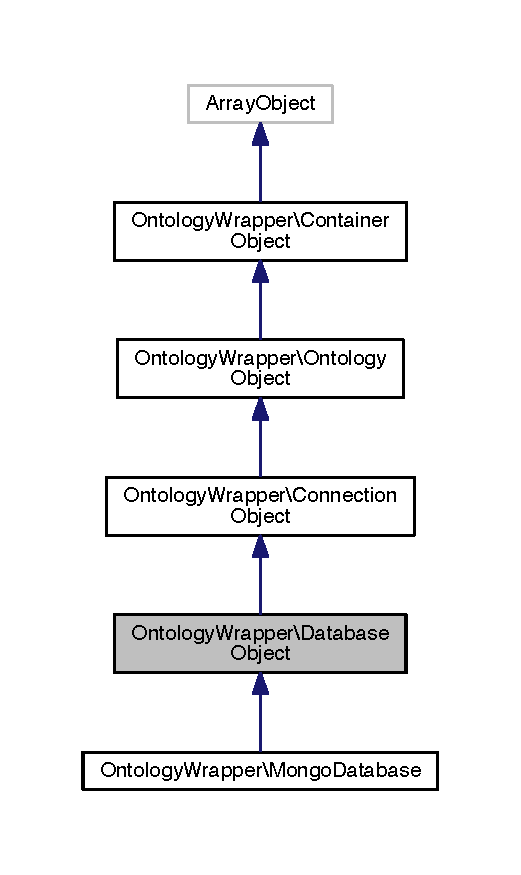
\includegraphics[width=250pt]{class_ontology_wrapper_1_1_database_object__inherit__graph}
\end{center}
\end{figure}


Collaboration diagram for Ontology\-Wrapper\textbackslash{}Database\-Object\-:\nopagebreak
\begin{figure}[H]
\begin{center}
\leavevmode
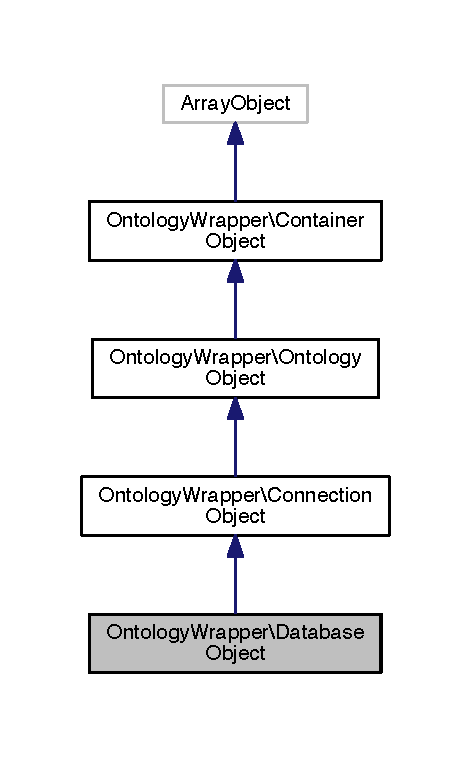
\includegraphics[width=226pt]{class_ontology_wrapper_1_1_database_object__coll__graph}
\end{center}
\end{figure}
\subsection*{Public Member Functions}
\begin{DoxyCompactItemize}
\item 
\hyperlink{class_ontology_wrapper_1_1_database_object_a12746bd4b3a9a869544ccaa06cf3bf34}{\-\_\-\-\_\-construct} (\$the\-Parameter=N\-U\-L\-L, \$the\-Parent=N\-U\-L\-L)
\item 
\hyperlink{class_ontology_wrapper_1_1_database_object_a0a3f541e719b56e1191aaf75a0b58b03}{drop} ()
\item 
\hyperlink{class_ontology_wrapper_1_1_database_object_a58886acb97fd38139340f649f12254a5}{Collection} (\$the\-Name)
\item 
\hyperlink{class_ontology_wrapper_1_1_database_object_a23409291f9aebd68da532a77c5143a84}{get\-Collections} ()
\item 
\hyperlink{class_ontology_wrapper_1_1_database_object_a4c7bd0ce9eb62750ef1c84351ed565cd}{set\-Sequence\-Number} (\$the\-Sequence, \$the\-Number=1)
\item 
\hyperlink{class_ontology_wrapper_1_1_database_object_ab731d606a297f2b1980f457efa1bc80d}{get\-Sequence\-Number} (\$the\-Sequence)
\end{DoxyCompactItemize}
\subsection*{Static Public Attributes}
\begin{DoxyCompactItemize}
\item 
\hypertarget{class_ontology_wrapper_1_1_database_object_a28b9a48fa04bbf9c64e584b99ada9704}{static {\bfseries \$s\-Offsets} = array( k\-T\-A\-G\-\_\-\-C\-O\-N\-N\-\_\-\-B\-A\-S\-E )}\label{class_ontology_wrapper_1_1_database_object_a28b9a48fa04bbf9c64e584b99ada9704}

\end{DoxyCompactItemize}
\subsection*{Protected Member Functions}
\begin{DoxyCompactItemize}
\item 
\hyperlink{class_ontology_wrapper_1_1_database_object_aa145306a1c58b9469d04dd17daa7fdbb}{new\-Server} (\$the\-Parameter)
\item 
\hyperlink{class_ontology_wrapper_1_1_database_object_aa72c5ba47e852c983f746aa95ec06c1d}{new\-Collection} (\$the\-Offsets)
\end{DoxyCompactItemize}
\subsection*{Additional Inherited Members}


\subsection{Detailed Description}
Database object

This {\itshape abstract} class is the ancestor of all classes representing database connection instances, this class extends the \hyperlink{class_ontology_wrapper_1_1_connection_object}{Connection\-Object} class to implement database specific functionality prototypes. \begin{DoxyVerb} @author            Milko A. Škofič <m.skofic@cgiar.org>
 @version   1.00 06/02/2014\end{DoxyVerb}
 

\subsection{Constructor \& Destructor Documentation}
\hypertarget{class_ontology_wrapper_1_1_database_object_a12746bd4b3a9a869544ccaa06cf3bf34}{\index{Ontology\-Wrapper\-::\-Database\-Object@{Ontology\-Wrapper\-::\-Database\-Object}!\-\_\-\-\_\-construct@{\-\_\-\-\_\-construct}}
\index{\-\_\-\-\_\-construct@{\-\_\-\-\_\-construct}!OntologyWrapper::DatabaseObject@{Ontology\-Wrapper\-::\-Database\-Object}}
\subsubsection[{\-\_\-\-\_\-construct}]{\setlength{\rightskip}{0pt plus 5cm}Ontology\-Wrapper\textbackslash{}\-Database\-Object\-::\-\_\-\-\_\-construct (
\begin{DoxyParamCaption}
\item[{}]{\$the\-Parameter = {\ttfamily NULL}, }
\item[{}]{\$the\-Parent = {\ttfamily NULL}}
\end{DoxyParamCaption}
)}}\label{class_ontology_wrapper_1_1_database_object_a12746bd4b3a9a869544ccaa06cf3bf34}
Instantiate class.

We overload the constructor to instantiate a server from the provided parameter, if the parent object was not provided, and set it as the parent.


\begin{DoxyParams}[1]{Parameters}
mixed & {\em \$the\-Parameter} & Data source name or parameters. \\
\hline
\hyperlink{class_ontology_wrapper_1_1_connection_object}{Connection\-Object} & {\em \$the\-Parent} & Connection parent.\\
\hline
\end{DoxyParams}
public

\begin{DoxySeeAlso}{See Also}
Server\-Object\-::\$s\-Offsets
\end{DoxySeeAlso}
\hyperlink{class_ontology_wrapper_1_1_database_object_aa145306a1c58b9469d04dd17daa7fdbb}{new\-Server()} 

\subsection{Member Function Documentation}
\hypertarget{class_ontology_wrapper_1_1_database_object_a58886acb97fd38139340f649f12254a5}{\index{Ontology\-Wrapper\-::\-Database\-Object@{Ontology\-Wrapper\-::\-Database\-Object}!Collection@{Collection}}
\index{Collection@{Collection}!OntologyWrapper::DatabaseObject@{Ontology\-Wrapper\-::\-Database\-Object}}
\subsubsection[{Collection}]{\setlength{\rightskip}{0pt plus 5cm}Ontology\-Wrapper\textbackslash{}\-Database\-Object\-::\-Collection (
\begin{DoxyParamCaption}
\item[{}]{\$the\-Name}
\end{DoxyParamCaption}
)}}\label{class_ontology_wrapper_1_1_database_object_a58886acb97fd38139340f649f12254a5}
Return collection connection

This method can be used to return a collection connection from the current database.

The method expects a single parameter which represents the collection name, the method should return an instance of a class derived from \hyperlink{class_ontology_wrapper_1_1_collection_object}{Collection\-Object}.


\begin{DoxyParams}[1]{Parameters}
string & {\em \$the\-Name} & Collection name.\\
\hline
\end{DoxyParams}
public \begin{DoxyReturn}{Returns}
\hyperlink{class_ontology_wrapper_1_1_collection_object}{Collection\-Object} Collection object.
\end{DoxyReturn}
\hyperlink{class_ontology_wrapper_1_1_database_object_aa72c5ba47e852c983f746aa95ec06c1d}{new\-Collection()} \hypertarget{class_ontology_wrapper_1_1_database_object_a0a3f541e719b56e1191aaf75a0b58b03}{\index{Ontology\-Wrapper\-::\-Database\-Object@{Ontology\-Wrapper\-::\-Database\-Object}!drop@{drop}}
\index{drop@{drop}!OntologyWrapper::DatabaseObject@{Ontology\-Wrapper\-::\-Database\-Object}}
\subsubsection[{drop}]{\setlength{\rightskip}{0pt plus 5cm}Ontology\-Wrapper\textbackslash{}\-Database\-Object\-::drop (
\begin{DoxyParamCaption}
{}
\end{DoxyParamCaption}
)\hspace{0.3cm}{\ttfamily [abstract]}}}\label{class_ontology_wrapper_1_1_database_object_a0a3f541e719b56e1191aaf75a0b58b03}
Drop the database

This method should drop the current database.

public \hypertarget{class_ontology_wrapper_1_1_database_object_a23409291f9aebd68da532a77c5143a84}{\index{Ontology\-Wrapper\-::\-Database\-Object@{Ontology\-Wrapper\-::\-Database\-Object}!get\-Collections@{get\-Collections}}
\index{get\-Collections@{get\-Collections}!OntologyWrapper::DatabaseObject@{Ontology\-Wrapper\-::\-Database\-Object}}
\subsubsection[{get\-Collections}]{\setlength{\rightskip}{0pt plus 5cm}Ontology\-Wrapper\textbackslash{}\-Database\-Object\-::get\-Collections (
\begin{DoxyParamCaption}
{}
\end{DoxyParamCaption}
)}}\label{class_ontology_wrapper_1_1_database_object_a23409291f9aebd68da532a77c5143a84}
Return collection names

This method should return the list of collection names of the current database, the method should return the following retults\-:


\begin{DoxyItemize}
\item {\ttfamily N\-U\-L\-L}\-: The operation is not supported. 
\item {\ttfamily F\-A\-L\-S\-E}\-: The database is not connected. 
\item {\ttfamily array}\-: The database collection names. 
\end{DoxyItemize}

We implement the method in this class as a fall-\/back.

public \begin{DoxyReturn}{Returns}
array Server statistics or {\ttfamily N\-U\-L\-L} if unsupported. 
\end{DoxyReturn}
\hypertarget{class_ontology_wrapper_1_1_database_object_ab731d606a297f2b1980f457efa1bc80d}{\index{Ontology\-Wrapper\-::\-Database\-Object@{Ontology\-Wrapper\-::\-Database\-Object}!get\-Sequence\-Number@{get\-Sequence\-Number}}
\index{get\-Sequence\-Number@{get\-Sequence\-Number}!OntologyWrapper::DatabaseObject@{Ontology\-Wrapper\-::\-Database\-Object}}
\subsubsection[{get\-Sequence\-Number}]{\setlength{\rightskip}{0pt plus 5cm}Ontology\-Wrapper\textbackslash{}\-Database\-Object\-::get\-Sequence\-Number (
\begin{DoxyParamCaption}
\item[{}]{\$the\-Sequence}
\end{DoxyParamCaption}
)\hspace{0.3cm}{\ttfamily [abstract]}}}\label{class_ontology_wrapper_1_1_database_object_ab731d606a297f2b1980f457efa1bc80d}
Return sequence number

This method should return a sequence number associated to the provided parameter. This operation is equivalent to requesting an auto-\/number for a database.

Each time a sequence number is requested, the sequence seed is updated, so use this method only when the sequence is required.

If the sequence selector is not found, a new one will be created starting with the number {\ttfamily 1}, so, if you need to start with another number, use the \hyperlink{class_ontology_wrapper_1_1_database_object_a4c7bd0ce9eb62750ef1c84351ed565cd}{set\-Sequence\-Number()} before.

Derived classes must implement this method.


\begin{DoxyParams}[1]{Parameters}
string & {\em \$the\-Sequence} & Sequence selector.\\
\hline
\end{DoxyParams}
public \begin{DoxyReturn}{Returns}
integer Sequence number. 
\end{DoxyReturn}
\hypertarget{class_ontology_wrapper_1_1_database_object_aa72c5ba47e852c983f746aa95ec06c1d}{\index{Ontology\-Wrapper\-::\-Database\-Object@{Ontology\-Wrapper\-::\-Database\-Object}!new\-Collection@{new\-Collection}}
\index{new\-Collection@{new\-Collection}!OntologyWrapper::DatabaseObject@{Ontology\-Wrapper\-::\-Database\-Object}}
\subsubsection[{new\-Collection}]{\setlength{\rightskip}{0pt plus 5cm}Ontology\-Wrapper\textbackslash{}\-Database\-Object\-::new\-Collection (
\begin{DoxyParamCaption}
\item[{}]{\$the\-Offsets}
\end{DoxyParamCaption}
)\hspace{0.3cm}{\ttfamily [abstract]}, {\ttfamily [protected]}}}\label{class_ontology_wrapper_1_1_database_object_aa72c5ba47e852c983f746aa95ec06c1d}
Return a new collection instance

This method should be implemented by concrete derived classes, it expects a list of offsets which include database information and should use them to instantiate a \hyperlink{class_ontology_wrapper_1_1_collection_object}{Collection\-Object} instance.

Derived classes must implement this method.


\begin{DoxyParams}[1]{Parameters}
array & {\em \$the\-Offsets} & Full collection offsets.\\
\hline
\end{DoxyParams}
protected \begin{DoxyReturn}{Returns}
\hyperlink{class_ontology_wrapper_1_1_collection_object}{Collection\-Object} Collection instance. 
\end{DoxyReturn}
\hypertarget{class_ontology_wrapper_1_1_database_object_aa145306a1c58b9469d04dd17daa7fdbb}{\index{Ontology\-Wrapper\-::\-Database\-Object@{Ontology\-Wrapper\-::\-Database\-Object}!new\-Server@{new\-Server}}
\index{new\-Server@{new\-Server}!OntologyWrapper::DatabaseObject@{Ontology\-Wrapper\-::\-Database\-Object}}
\subsubsection[{new\-Server}]{\setlength{\rightskip}{0pt plus 5cm}Ontology\-Wrapper\textbackslash{}\-Database\-Object\-::new\-Server (
\begin{DoxyParamCaption}
\item[{}]{\$the\-Parameter}
\end{DoxyParamCaption}
)\hspace{0.3cm}{\ttfamily [abstract]}, {\ttfamily [protected]}}}\label{class_ontology_wrapper_1_1_database_object_aa145306a1c58b9469d04dd17daa7fdbb}
Return a new server instance

This method should be implemented by concrete derived classes, it expects a list of offsets or a data source name containing the necessary elements to instantiate a \hyperlink{class_ontology_wrapper_1_1_server_object}{Server\-Object} instance which will be considered the current object's parent.

Derived classes must implement this method.


\begin{DoxyParams}[1]{Parameters}
mixed & {\em \$the\-Parameter} & Server parameters.\\
\hline
\end{DoxyParams}
protected \begin{DoxyReturn}{Returns}
\hyperlink{class_ontology_wrapper_1_1_server_object}{Server\-Object} Server instance. 
\end{DoxyReturn}
\hypertarget{class_ontology_wrapper_1_1_database_object_a4c7bd0ce9eb62750ef1c84351ed565cd}{\index{Ontology\-Wrapper\-::\-Database\-Object@{Ontology\-Wrapper\-::\-Database\-Object}!set\-Sequence\-Number@{set\-Sequence\-Number}}
\index{set\-Sequence\-Number@{set\-Sequence\-Number}!OntologyWrapper::DatabaseObject@{Ontology\-Wrapper\-::\-Database\-Object}}
\subsubsection[{set\-Sequence\-Number}]{\setlength{\rightskip}{0pt plus 5cm}Ontology\-Wrapper\textbackslash{}\-Database\-Object\-::set\-Sequence\-Number (
\begin{DoxyParamCaption}
\item[{}]{\$the\-Sequence, }
\item[{}]{\$the\-Number = {\ttfamily 1}}
\end{DoxyParamCaption}
)\hspace{0.3cm}{\ttfamily [abstract]}}}\label{class_ontology_wrapper_1_1_database_object_a4c7bd0ce9eb62750ef1c84351ed565cd}
Set sequence number

This method should initialise a sequence number associated to the provided parameter. This operation is equivalent to resetting an auto-\/number for a database.

Once the sequence is set, the next requested sequence number will hold the value set by this method, so to start counting from {\ttfamily 1} you should provide this value to this method.

Derived classes must implement this method.


\begin{DoxyParams}[1]{Parameters}
string & {\em \$the\-Sequence} & Sequence selector. \\
\hline
integer & {\em \$the\-Number} & Sequence number.\\
\hline
\end{DoxyParams}
public 

The documentation for this class was generated from the following file\-:\begin{DoxyCompactItemize}
\item 
/\-Library/\-Web\-Server/\-Library/\-Ontology\-Wrapper/\-Library/\-Ontology\-Wrapper/Database\-Object.\-php\end{DoxyCompactItemize}

\hypertarget{class_ontology_wrapper_1_1_dictionary}{\section{Ontology\-Wrapper\textbackslash{}Dictionary Class Reference}
\label{class_ontology_wrapper_1_1_dictionary}\index{Ontology\-Wrapper\textbackslash{}\-Dictionary@{Ontology\-Wrapper\textbackslash{}\-Dictionary}}
}


Inheritance diagram for Ontology\-Wrapper\textbackslash{}Dictionary\-:
\nopagebreak
\begin{figure}[H]
\begin{center}
\leavevmode
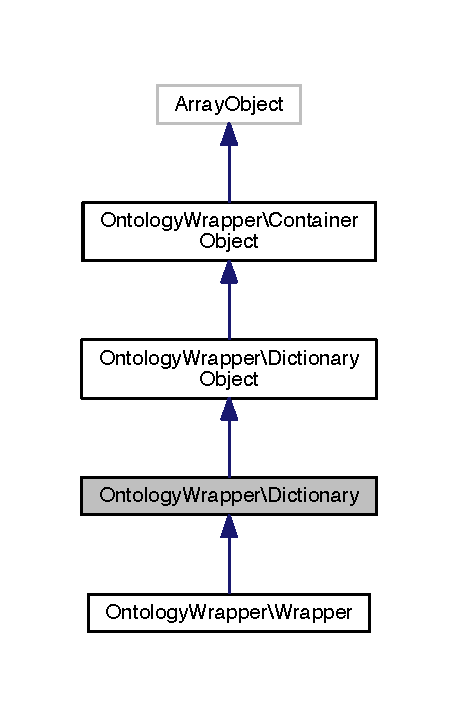
\includegraphics[width=220pt]{class_ontology_wrapper_1_1_dictionary__inherit__graph}
\end{center}
\end{figure}


Collaboration diagram for Ontology\-Wrapper\textbackslash{}Dictionary\-:
\nopagebreak
\begin{figure}[H]
\begin{center}
\leavevmode
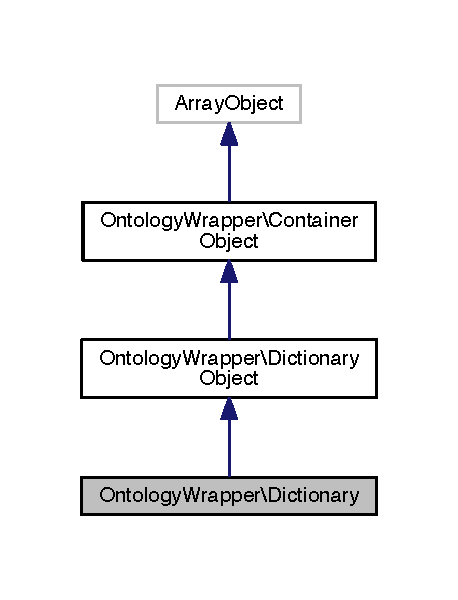
\includegraphics[width=220pt]{class_ontology_wrapper_1_1_dictionary__coll__graph}
\end{center}
\end{figure}
\subsection*{Public Member Functions}
\begin{DoxyCompactItemize}
\item 
\hyperlink{class_ontology_wrapper_1_1_dictionary_a9b2c726ae5c9c19298f3bfc96b07dd5a}{\-\_\-\-\_\-construct} (\$the\-Identifier, \$the\-Servers=N\-U\-L\-L)
\end{DoxyCompactItemize}
\subsection*{Additional Inherited Members}


\subsection{Detailed Description}
\hyperlink{class_ontology_wrapper_1_1_dictionary}{Dictionary}

This class implements a {\itshape concrete} instance of the \hyperlink{class_ontology_wrapper_1_1_dictionary_object}{Dictionary\-Object} class which uses the \hyperlink{}{Memcached\-Dictionary} trait to implement the dictionary cache.

This class implements a constructor which expects the \hyperlink{}{Memcached} persistent identifier and the list of servers. \begin{DoxyVerb} @author            Milko A. Škofič <m.skofic@cgiar.org>
 @version   1.00 16/02/2014\end{DoxyVerb}
 

\subsection{Constructor \& Destructor Documentation}
\hypertarget{class_ontology_wrapper_1_1_dictionary_a9b2c726ae5c9c19298f3bfc96b07dd5a}{\index{Ontology\-Wrapper\-::\-Dictionary@{Ontology\-Wrapper\-::\-Dictionary}!\-\_\-\-\_\-construct@{\-\_\-\-\_\-construct}}
\index{\-\_\-\-\_\-construct@{\-\_\-\-\_\-construct}!OntologyWrapper::Dictionary@{Ontology\-Wrapper\-::\-Dictionary}}
\subsubsection[{\-\_\-\-\_\-construct}]{\setlength{\rightskip}{0pt plus 5cm}Ontology\-Wrapper\textbackslash{}\-Dictionary\-::\-\_\-\-\_\-construct (
\begin{DoxyParamCaption}
\item[{}]{\$the\-Identifier, }
\item[{}]{\$the\-Servers = {\ttfamily NULL}}
\end{DoxyParamCaption}
)}}\label{class_ontology_wrapper_1_1_dictionary_a9b2c726ae5c9c19298f3bfc96b07dd5a}
Instantiate class.

The constructor accepts two parameters\-:


\begin{DoxyItemize}
\item {\bfseries \$the\-Identifier}\-: This string parameter represents the \{ Memcached\} persistent identifier provided to its constructor, the parameter is required, since the cache should be active across sessions. 
\item {\bfseries \$the\-Servers}\-: This array parameter represents the list of servers that serve the cache, it is equivalent to the parameter of the \hyperlink{}{Memcached\-::add\-Servers()} method, it is a list of elements comprised by three parameters\-: 
\begin{DoxyItemize}
\item {\itshape Host}\-: The server host. 
\item {\itshape Port}\-: The server port. 
\item {\itshape Weight}\-: The weight of the server relative to the total weight of all the servers in the pool. 
\end{DoxyItemize}This parameter may be omitted if the cache has been instantiate elsewhere with the same persistent identifier. 
\end{DoxyItemize}

The constructor will first instantiate the \hyperlink{}{Memcached} object, then it will check if the connection resource has already a list of servers associated, if that is the case we assume the cache is already initialised; if that is not the case, we will add the servers provided in the second parameter.


\begin{DoxyParams}[1]{Parameters}
mixed & {\em \$the\-Identifier} & Persistent identifier. \\
\hline
array & {\em \$the\-Servers} & List of servers.\\
\hline
\end{DoxyParams}
public


\begin{DoxyExceptions}{Exceptions}
{\em Exception} & init() \\
\hline
\end{DoxyExceptions}


The documentation for this class was generated from the following file\-:\begin{DoxyCompactItemize}
\item 
/\-Library/\-Web\-Server/\-Library/\-Ontology\-Wrapper/\-Library/\-Ontology\-Wrapper/Dictionary.\-php\end{DoxyCompactItemize}

\hypertarget{class_ontology_wrapper_1_1_dictionary_object}{\section{Ontology\-Wrapper\textbackslash{}Dictionary\-Object Class Reference}
\label{class_ontology_wrapper_1_1_dictionary_object}\index{Ontology\-Wrapper\textbackslash{}\-Dictionary\-Object@{Ontology\-Wrapper\textbackslash{}\-Dictionary\-Object}}
}


Inheritance diagram for Ontology\-Wrapper\textbackslash{}Dictionary\-Object\-:
\nopagebreak
\begin{figure}[H]
\begin{center}
\leavevmode
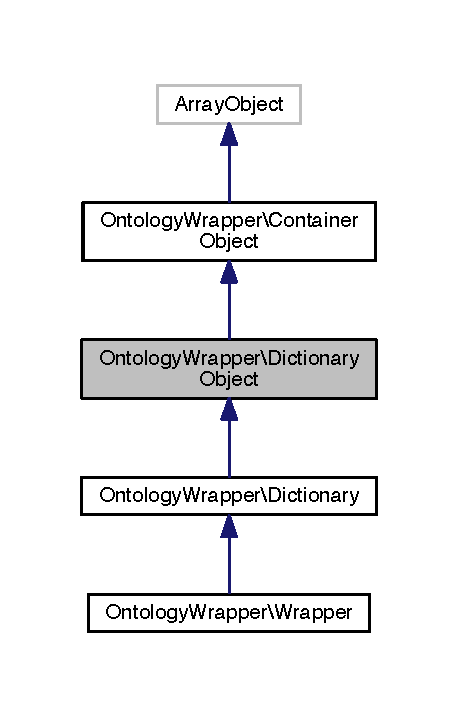
\includegraphics[width=220pt]{class_ontology_wrapper_1_1_dictionary_object__inherit__graph}
\end{center}
\end{figure}


Collaboration diagram for Ontology\-Wrapper\textbackslash{}Dictionary\-Object\-:
\nopagebreak
\begin{figure}[H]
\begin{center}
\leavevmode
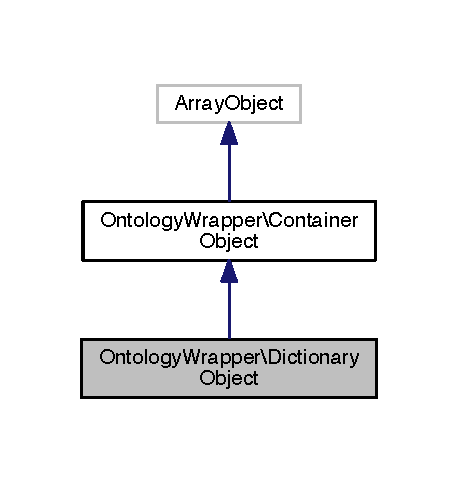
\includegraphics[width=220pt]{class_ontology_wrapper_1_1_dictionary_object__coll__graph}
\end{center}
\end{figure}
\subsection*{Public Member Functions}
\begin{DoxyCompactItemize}
\item 
\hyperlink{class_ontology_wrapper_1_1_dictionary_object_afc377ae7487d9f7004f0f790121b9f76}{cache} ()
\item 
\hyperlink{class_ontology_wrapper_1_1_dictionary_object_a34c06436a94921b47885505cfd5efffe}{set\-Tag} (\$the\-Tag, \$the\-Life=0)
\item 
\hyperlink{class_ontology_wrapper_1_1_dictionary_object_a9e86ec29b5523074af3244888789e64e}{get\-Identifier} (\$the\-Identifier, \$do\-Assert=T\-R\-U\-E)
\item 
\hyperlink{class_ontology_wrapper_1_1_dictionary_object_a10ca50e087c2d9b4ff6da952088e9195}{get\-Object} (\$the\-Identifier, \$do\-Assert=T\-R\-U\-E)
\item 
\hyperlink{class_ontology_wrapper_1_1_dictionary_object_a263aeb948e7668950fc9aa90be459558}{del\-Tag} (\$the\-Identifier, \$do\-Assert=F\-A\-L\-S\-E)
\item 
\hyperlink{class_ontology_wrapper_1_1_dictionary_object_ab2ae4af97de01b93c8c89fdfe6a2cfad}{dictionary\-Filled} ()
\item 
\hyperlink{class_ontology_wrapper_1_1_dictionary_object_a8f3fa4a572053a970eda952c9f76ae3b}{dictionary\-Flush} (\$the\-Delay=0)
\end{DoxyCompactItemize}
\subsection*{Protected Member Functions}
\begin{DoxyCompactItemize}
\item 
\hyperlink{class_ontology_wrapper_1_1_dictionary_object_a29d05a749afc71b7a09702f6bc7a8f17}{set\-Entry} (\$the\-Key, \$the\-Value, \$the\-Life)
\item 
\hyperlink{class_ontology_wrapper_1_1_dictionary_object_ab6c1db9ac69974aa12940468bb1e95c4}{get\-Entry} (\$the\-Key)
\item 
\hyperlink{class_ontology_wrapper_1_1_dictionary_object_a2af5d68ce5b9187dbc6963f71de4274a}{del\-Entry} (\$the\-Key)
\end{DoxyCompactItemize}
\subsection*{Protected Attributes}
\begin{DoxyCompactItemize}
\item 
\hypertarget{class_ontology_wrapper_1_1_dictionary_object_afcd8452895d2b22850c042465a1228fc}{{\bfseries \$m\-Pid} = N\-U\-L\-L}\label{class_ontology_wrapper_1_1_dictionary_object_afcd8452895d2b22850c042465a1228fc}

\item 
\hypertarget{class_ontology_wrapper_1_1_dictionary_object_ad57b4dc0623434edf61cfd7660a26b8c}{{\bfseries \$m\-Cache} = N\-U\-L\-L}\label{class_ontology_wrapper_1_1_dictionary_object_ad57b4dc0623434edf61cfd7660a26b8c}

\end{DoxyCompactItemize}
\subsection*{Additional Inherited Members}


\subsection{Detailed Description}
\hyperlink{class_ontology_wrapper_1_1_dictionary}{Dictionary} object

A {\itshape dictionary} is used to {\itshape identify} and {\itshape document} data properties. The dictionary stores a set of objects called {\itshape tags}, which contain all the necessary information needed to understand what a specific data property is, how it can be used, what data types it can take and all the information necessary to manage it.

Tags are identified in two ways\-: with their {\itshape persistent identifier}, which is a {\itshape string} that uniquely identifies the tag across all dictionaries, and with their {\itshape serial identifier}, which is an {\itshape integer} that uniquely identifies the tag only within the current dictionary.

All persistent data properties of all objects of this library are {\itshape serial identifiers of tag objects}. This dictionary provides the abiliti to convert among persistent and serial identifiers, and it provides the ability to retrieve tag objects.

The dictionary is essentially a cache that allows fast access to the tag elements of the ontology, the dictionary allows retrieving the serial identifier given a persistent identifier, or retrieve a tag object given a serial identifier.

Derived classes must implement the constructor and the protected dictionary interface. \begin{DoxyVerb} @author            Milko A. Škofič <m.skofic@cgiar.org>
 @version   1.00 16/02/2014\end{DoxyVerb}
 

\subsection{Member Function Documentation}
\hypertarget{class_ontology_wrapper_1_1_dictionary_object_afc377ae7487d9f7004f0f790121b9f76}{\index{Ontology\-Wrapper\-::\-Dictionary\-Object@{Ontology\-Wrapper\-::\-Dictionary\-Object}!cache@{cache}}
\index{cache@{cache}!OntologyWrapper::DictionaryObject@{Ontology\-Wrapper\-::\-Dictionary\-Object}}
\subsubsection[{cache}]{\setlength{\rightskip}{0pt plus 5cm}Ontology\-Wrapper\textbackslash{}\-Dictionary\-Object\-::cache (
\begin{DoxyParamCaption}
{}
\end{DoxyParamCaption}
)}}\label{class_ontology_wrapper_1_1_dictionary_object_afc377ae7487d9f7004f0f790121b9f76}
Return cache

This method will return the current cache.

public \hypertarget{class_ontology_wrapper_1_1_dictionary_object_a2af5d68ce5b9187dbc6963f71de4274a}{\index{Ontology\-Wrapper\-::\-Dictionary\-Object@{Ontology\-Wrapper\-::\-Dictionary\-Object}!del\-Entry@{del\-Entry}}
\index{del\-Entry@{del\-Entry}!OntologyWrapper::DictionaryObject@{Ontology\-Wrapper\-::\-Dictionary\-Object}}
\subsubsection[{del\-Entry}]{\setlength{\rightskip}{0pt plus 5cm}Ontology\-Wrapper\textbackslash{}\-Dictionary\-Object\-::del\-Entry (
\begin{DoxyParamCaption}
\item[{}]{\$the\-Key}
\end{DoxyParamCaption}
)\hspace{0.3cm}{\ttfamily [abstract]}, {\ttfamily [protected]}}}\label{class_ontology_wrapper_1_1_dictionary_object_a2af5d68ce5b9187dbc6963f71de4274a}
Get a dictionary entry

This method should delete the dictionary entry corresponding to the provided key; if the entry was deleted, the method should return {\ttfamily T\-R\-U\-E}, if the entry was not found, the method should return {\ttfamily F\-A\-L\-S\-E}.

If the operation fails the method should raise an exception.


\begin{DoxyParams}[1]{Parameters}
mixed & {\em \$the\-Key} & Entry key.\\
\hline
\end{DoxyParams}
protected \begin{DoxyReturn}{Returns}
boolean {\ttfamily T\-R\-U\-E} deleted, {\ttfamily F\-A\-L\-S\-E} not matched. 
\end{DoxyReturn}
\hypertarget{class_ontology_wrapper_1_1_dictionary_object_a263aeb948e7668950fc9aa90be459558}{\index{Ontology\-Wrapper\-::\-Dictionary\-Object@{Ontology\-Wrapper\-::\-Dictionary\-Object}!del\-Tag@{del\-Tag}}
\index{del\-Tag@{del\-Tag}!OntologyWrapper::DictionaryObject@{Ontology\-Wrapper\-::\-Dictionary\-Object}}
\subsubsection[{del\-Tag}]{\setlength{\rightskip}{0pt plus 5cm}Ontology\-Wrapper\textbackslash{}\-Dictionary\-Object\-::del\-Tag (
\begin{DoxyParamCaption}
\item[{}]{\$the\-Identifier, }
\item[{}]{\$do\-Assert = {\ttfamily FALSE}}
\end{DoxyParamCaption}
)}}\label{class_ontology_wrapper_1_1_dictionary_object_a263aeb948e7668950fc9aa90be459558}
Delete tag

This method should delete a tag entry corresponding to the provided persistent or serial identifier. This means that the method will delete both the identifier and the object entries.

Note that an integer identifier is assumed to be the serial identifier and anything else will be cast to string and assumed to be the persistent identifier.

The second parameter rperesents a boolean flag\-: if {\ttfamily T\-R\-U\-E} and the provided identifier is not matched, the method will raise an exception. By default this option is {\ttfamily F\-A\-L\-S\-E}.


\begin{DoxyParams}[1]{Parameters}
mixed & {\em \$the\-Identifier} & Persistent or serial identifier. \\
\hline
boolean & {\em \$do\-Assert} & If {\ttfamily T\-R\-U\-E} assert match.\\
\hline
\end{DoxyParams}
public

\hyperlink{class_ontology_wrapper_1_1_dictionary_object_a2af5d68ce5b9187dbc6963f71de4274a}{del\-Entry()} \begin{DoxyReturn}{Returns}
boolean {\ttfamily T\-R\-U\-E} deleted, {\ttfamily F\-A\-L\-S\-E} not found. 
\end{DoxyReturn}
\hypertarget{class_ontology_wrapper_1_1_dictionary_object_ab2ae4af97de01b93c8c89fdfe6a2cfad}{\index{Ontology\-Wrapper\-::\-Dictionary\-Object@{Ontology\-Wrapper\-::\-Dictionary\-Object}!dictionary\-Filled@{dictionary\-Filled}}
\index{dictionary\-Filled@{dictionary\-Filled}!OntologyWrapper::DictionaryObject@{Ontology\-Wrapper\-::\-Dictionary\-Object}}
\subsubsection[{dictionary\-Filled}]{\setlength{\rightskip}{0pt plus 5cm}Ontology\-Wrapper\textbackslash{}\-Dictionary\-Object\-::dictionary\-Filled (
\begin{DoxyParamCaption}
{}
\end{DoxyParamCaption}
)}}\label{class_ontology_wrapper_1_1_dictionary_object_ab2ae4af97de01b93c8c89fdfe6a2cfad}
Check if dictionary is filled

This method will return {\ttfamily T\-R\-U\-E} if the current dictionary can resolve the {\ttfamily k\-T\-A\-G\-\_\-\-D\-O\-M\-A\-I\-N} identifier.

We assume that if the dictionary can resolve this identifier, it means it must be filled.

public \begin{DoxyReturn}{Returns}
boolean {\ttfamily T\-R\-U\-E} means filled. 
\end{DoxyReturn}
\hypertarget{class_ontology_wrapper_1_1_dictionary_object_a8f3fa4a572053a970eda952c9f76ae3b}{\index{Ontology\-Wrapper\-::\-Dictionary\-Object@{Ontology\-Wrapper\-::\-Dictionary\-Object}!dictionary\-Flush@{dictionary\-Flush}}
\index{dictionary\-Flush@{dictionary\-Flush}!OntologyWrapper::DictionaryObject@{Ontology\-Wrapper\-::\-Dictionary\-Object}}
\subsubsection[{dictionary\-Flush}]{\setlength{\rightskip}{0pt plus 5cm}Ontology\-Wrapper\textbackslash{}\-Dictionary\-Object\-::dictionary\-Flush (
\begin{DoxyParamCaption}
\item[{}]{\$the\-Delay = {\ttfamily 0}}
\end{DoxyParamCaption}
)\hspace{0.3cm}{\ttfamily [abstract]}}}\label{class_ontology_wrapper_1_1_dictionary_object_a8f3fa4a572053a970eda952c9f76ae3b}
Flush dictionary elements

This method should invalidate all the elements of the dictionary.

The method expects one parameter that corresponds to the delay in seconds before the elements will be invalidated.


\begin{DoxyParams}[1]{Parameters}
integer & {\em \$the\-Delay} & Delay before flush.\\
\hline
\end{DoxyParams}
public \hypertarget{class_ontology_wrapper_1_1_dictionary_object_ab6c1db9ac69974aa12940468bb1e95c4}{\index{Ontology\-Wrapper\-::\-Dictionary\-Object@{Ontology\-Wrapper\-::\-Dictionary\-Object}!get\-Entry@{get\-Entry}}
\index{get\-Entry@{get\-Entry}!OntologyWrapper::DictionaryObject@{Ontology\-Wrapper\-::\-Dictionary\-Object}}
\subsubsection[{get\-Entry}]{\setlength{\rightskip}{0pt plus 5cm}Ontology\-Wrapper\textbackslash{}\-Dictionary\-Object\-::get\-Entry (
\begin{DoxyParamCaption}
\item[{}]{\$the\-Key}
\end{DoxyParamCaption}
)\hspace{0.3cm}{\ttfamily [abstract]}, {\ttfamily [protected]}}}\label{class_ontology_wrapper_1_1_dictionary_object_ab6c1db9ac69974aa12940468bb1e95c4}
Get a dictionary entry

This method should return the dictionary entry corresponding to the provided key; if the entry is not matched, the method should return {\ttfamily N\-U\-L\-L}.

If the operation fails the method should raise an exception.


\begin{DoxyParams}[1]{Parameters}
mixed & {\em \$the\-Key} & Entry key.\\
\hline
\end{DoxyParams}
protected \begin{DoxyReturn}{Returns}
mixed Entry value or {\ttfamily N\-U\-L\-L}. 
\end{DoxyReturn}
\hypertarget{class_ontology_wrapper_1_1_dictionary_object_a9e86ec29b5523074af3244888789e64e}{\index{Ontology\-Wrapper\-::\-Dictionary\-Object@{Ontology\-Wrapper\-::\-Dictionary\-Object}!get\-Identifier@{get\-Identifier}}
\index{get\-Identifier@{get\-Identifier}!OntologyWrapper::DictionaryObject@{Ontology\-Wrapper\-::\-Dictionary\-Object}}
\subsubsection[{get\-Identifier}]{\setlength{\rightskip}{0pt plus 5cm}Ontology\-Wrapper\textbackslash{}\-Dictionary\-Object\-::get\-Identifier (
\begin{DoxyParamCaption}
\item[{}]{\$the\-Identifier, }
\item[{}]{\$do\-Assert = {\ttfamily TRUE}}
\end{DoxyParamCaption}
)}}\label{class_ontology_wrapper_1_1_dictionary_object_a9e86ec29b5523074af3244888789e64e}
Get identifier

This method should return the serial identifier corresponding to the provided persistent identifier.

The second parameter represents a boolean flag\-: if {\ttfamily T\-R\-U\-E} and the provided identifier is not matched, the method will raise an exception; if {\ttfamily F\-A\-L\-S\-E}, the method will return {\ttfamily N\-U\-L\-L} on a mismatch. By default this option is {\ttfamily T\-R\-U\-E}.


\begin{DoxyParams}[1]{Parameters}
string & {\em \$the\-Identifier} & Persistent identifier. \\
\hline
boolean & {\em \$do\-Assert} & If {\ttfamily T\-R\-U\-E} assert match.\\
\hline
\end{DoxyParams}
public \begin{DoxyReturn}{Returns}
mixed Native identifier or {\ttfamily N\-U\-L\-L}.
\begin{DoxyItemize}
\item 
\item 
\end{DoxyItemize}
\end{DoxyReturn}

\begin{DoxyExceptions}{Exceptions}
{\em Exception} & \hyperlink{class_ontology_wrapper_1_1_dictionary_object_ab6c1db9ac69974aa12940468bb1e95c4}{get\-Entry()} \\
\hline
\end{DoxyExceptions}
\hypertarget{class_ontology_wrapper_1_1_dictionary_object_a10ca50e087c2d9b4ff6da952088e9195}{\index{Ontology\-Wrapper\-::\-Dictionary\-Object@{Ontology\-Wrapper\-::\-Dictionary\-Object}!get\-Object@{get\-Object}}
\index{get\-Object@{get\-Object}!OntologyWrapper::DictionaryObject@{Ontology\-Wrapper\-::\-Dictionary\-Object}}
\subsubsection[{get\-Object}]{\setlength{\rightskip}{0pt plus 5cm}Ontology\-Wrapper\textbackslash{}\-Dictionary\-Object\-::get\-Object (
\begin{DoxyParamCaption}
\item[{}]{\$the\-Identifier, }
\item[{}]{\$do\-Assert = {\ttfamily TRUE}}
\end{DoxyParamCaption}
)}}\label{class_ontology_wrapper_1_1_dictionary_object_a10ca50e087c2d9b4ff6da952088e9195}
Get object

This method should return the tag object corresponding to the provided serial identifier.

The second parameter represents a boolean flag\-: if {\ttfamily T\-R\-U\-E} and the provided identifier is not matched, the method will raise an exception; if {\ttfamily F\-A\-L\-S\-E}, the method will return {\ttfamily N\-U\-L\-L} on a mismatch. By default this option is {\ttfamily T\-R\-U\-E}.


\begin{DoxyParams}[1]{Parameters}
integer & {\em \$the\-Identifier} & Serial identifier. \\
\hline
boolean & {\em \$do\-Assert} & If {\ttfamily T\-R\-U\-E} assert match.\\
\hline
\end{DoxyParams}
public \begin{DoxyReturn}{Returns}
mixed \hyperlink{class_ontology_wrapper_1_1_tag}{Tag} object array or {\ttfamily N\-U\-L\-L}.
\begin{DoxyItemize}
\item 
\item 
\end{DoxyItemize}
\end{DoxyReturn}

\begin{DoxyExceptions}{Exceptions}
{\em Exception} & \hyperlink{class_ontology_wrapper_1_1_dictionary_object_ab6c1db9ac69974aa12940468bb1e95c4}{get\-Entry()} \\
\hline
\end{DoxyExceptions}
\hypertarget{class_ontology_wrapper_1_1_dictionary_object_a29d05a749afc71b7a09702f6bc7a8f17}{\index{Ontology\-Wrapper\-::\-Dictionary\-Object@{Ontology\-Wrapper\-::\-Dictionary\-Object}!set\-Entry@{set\-Entry}}
\index{set\-Entry@{set\-Entry}!OntologyWrapper::DictionaryObject@{Ontology\-Wrapper\-::\-Dictionary\-Object}}
\subsubsection[{set\-Entry}]{\setlength{\rightskip}{0pt plus 5cm}Ontology\-Wrapper\textbackslash{}\-Dictionary\-Object\-::set\-Entry (
\begin{DoxyParamCaption}
\item[{}]{\$the\-Key, }
\item[{}]{\$the\-Value, }
\item[{}]{\$the\-Life}
\end{DoxyParamCaption}
)\hspace{0.3cm}{\ttfamily [abstract]}, {\ttfamily [protected]}}}\label{class_ontology_wrapper_1_1_dictionary_object_a29d05a749afc71b7a09702f6bc7a8f17}
Set a dictionary entry

This method should commit a new entry in the dictionary, if it doesn't exist yet, or replace the matching entry if it already exists.

The method expects the following parameters\-:


\begin{DoxyItemize}
\item {\bfseries \$the\-Key}\-: Entry key. 
\item {\bfseries \$the\-Value}\-: Entry value. 
\item {\bfseries \$the\-Life}\-: Entry lifetime in seconds, 0 means permanent. 
\end{DoxyItemize}

If the operation fails the method should raise an exception.


\begin{DoxyParams}[1]{Parameters}
mixed & {\em \$the\-Key} & Entry key. \\
\hline
mixed & {\em \$the\-Value} & Entry value. \\
\hline
integer & {\em \$the\-Life} & Entry lifetime.\\
\hline
\end{DoxyParams}
protected \hypertarget{class_ontology_wrapper_1_1_dictionary_object_a34c06436a94921b47885505cfd5efffe}{\index{Ontology\-Wrapper\-::\-Dictionary\-Object@{Ontology\-Wrapper\-::\-Dictionary\-Object}!set\-Tag@{set\-Tag}}
\index{set\-Tag@{set\-Tag}!OntologyWrapper::DictionaryObject@{Ontology\-Wrapper\-::\-Dictionary\-Object}}
\subsubsection[{set\-Tag}]{\setlength{\rightskip}{0pt plus 5cm}Ontology\-Wrapper\textbackslash{}\-Dictionary\-Object\-::set\-Tag (
\begin{DoxyParamCaption}
\item[{}]{\$the\-Tag, }
\item[{}]{\$the\-Life = {\ttfamily 0}}
\end{DoxyParamCaption}
)}}\label{class_ontology_wrapper_1_1_dictionary_object_a34c06436a94921b47885505cfd5efffe}
Set tag

This method should either commit the provided tag object, if it doesn't yet exist, or replace an existing tag object.

The method expects the following parameters\-:


\begin{DoxyItemize}
\item {\bfseries \$the\-Tag}\-: \hyperlink{class_ontology_wrapper_1_1_tag}{Tag} object, if derived from an array object, it will be converted into an array, before it is set into the dictionary. 
\item {\bfseries \$the\-Life}\-: Lifetime of the dictionary entry in seconds, 0 means permanent. 
\end{DoxyItemize}


\begin{DoxyParams}[1]{Parameters}
mixed & {\em \$the\-Tag} & \hyperlink{class_ontology_wrapper_1_1_tag}{Tag} object. \\
\hline
integer & {\em \$the\-Life} & Element lifetime.\\
\hline
\end{DoxyParams}
public
\begin{DoxyItemize}
\item 
\item 
\begin{DoxyExceptions}{Exceptions}
{\em Exception} & \hyperlink{class_ontology_wrapper_1_1_dictionary_object_a29d05a749afc71b7a09702f6bc7a8f17}{set\-Entry()} \\
\hline
\end{DoxyExceptions}

\end{DoxyItemize}

The documentation for this class was generated from the following file\-:\begin{DoxyCompactItemize}
\item 
/\-Library/\-Web\-Server/\-Library/\-Ontology\-Wrapper/\-Library/\-Ontology\-Wrapper/Dictionary\-Object.\-php\end{DoxyCompactItemize}

\hypertarget{class_ontology_wrapper_1_1_edge}{\section{Ontology\-Wrapper\textbackslash{}Edge Class Reference}
\label{class_ontology_wrapper_1_1_edge}\index{Ontology\-Wrapper\textbackslash{}\-Edge@{Ontology\-Wrapper\textbackslash{}\-Edge}}
}


Inheritance diagram for Ontology\-Wrapper\textbackslash{}Edge\-:\nopagebreak
\begin{figure}[H]
\begin{center}
\leavevmode
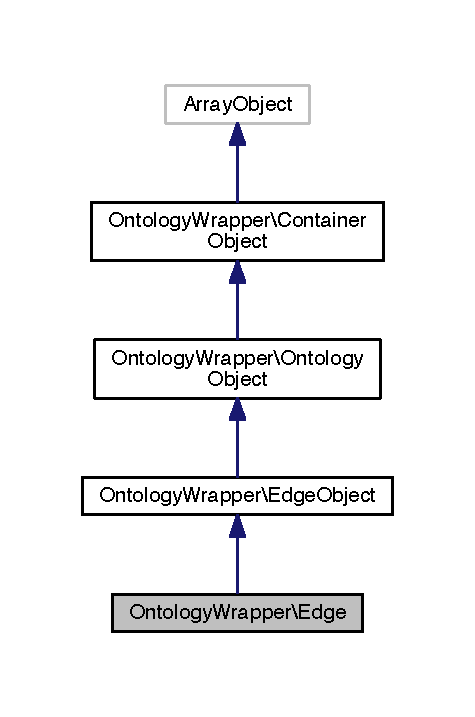
\includegraphics[width=228pt]{class_ontology_wrapper_1_1_edge__inherit__graph}
\end{center}
\end{figure}


Collaboration diagram for Ontology\-Wrapper\textbackslash{}Edge\-:\nopagebreak
\begin{figure}[H]
\begin{center}
\leavevmode
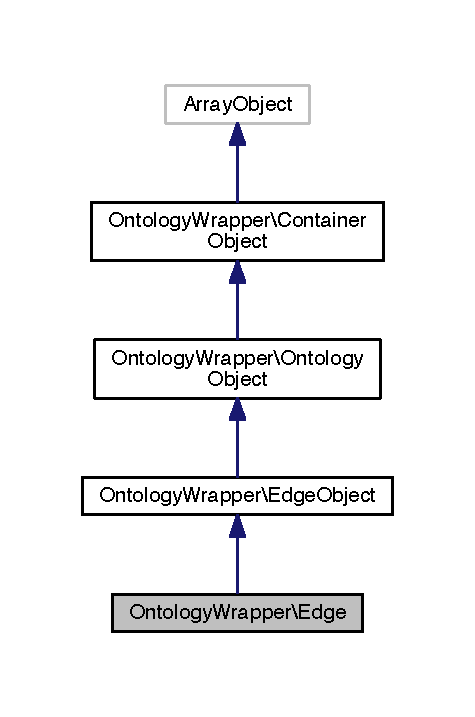
\includegraphics[width=228pt]{class_ontology_wrapper_1_1_edge__coll__graph}
\end{center}
\end{figure}
\subsection*{Public Member Functions}
\begin{DoxyCompactItemize}
\item 
\hyperlink{class_ontology_wrapper_1_1_edge_ae3ae5e6b59244535718879a98e4b16d3}{\-\_\-\-\_\-construct} (\$the\-Container=N\-U\-L\-L, \$the\-Identifier=N\-U\-L\-L)
\item 
\hyperlink{class_ontology_wrapper_1_1_edge_acd4c7e465ef4a809580d6ad8d19dd7ab}{load\-Subject} ()
\item 
\hyperlink{class_ontology_wrapper_1_1_edge_ab4ec3c0a5b1b89632c20c5d807e13da9}{load\-Predicate} ()
\item 
\hyperlink{class_ontology_wrapper_1_1_edge_ac0176e2db533a781fb59c60368e3f5e4}{load\-Object} ()
\item 
\hyperlink{class_ontology_wrapper_1_1_edge_aaf586277ed281c7303c4f7fafec2b7ac}{collect\-References} (\&\$the\-Container, \$do\-Object=T\-R\-U\-E)
\end{DoxyCompactItemize}
\subsection*{Static Public Member Functions}
\begin{DoxyCompactItemize}
\item 
static \hyperlink{class_ontology_wrapper_1_1_edge_a159dd13efea0442efae114c0903a3aeb}{Resolve\-Object} (\hyperlink{class_ontology_wrapper_1_1_connection_object}{Connection\-Object} \$the\-Connection, \$the\-Identifier, \$do\-Assert=T\-R\-U\-E)
\end{DoxyCompactItemize}
\subsection*{Public Attributes}
\begin{DoxyCompactItemize}
\item 
\hypertarget{class_ontology_wrapper_1_1_edge_af0a68ad0c816d7efde12dc4962ffa039}{const {\bfseries k\-S\-E\-Q\-\_\-\-N\-A\-M\-E} = '\-\_\-edges'}\label{class_ontology_wrapper_1_1_edge_af0a68ad0c816d7efde12dc4962ffa039}

\end{DoxyCompactItemize}
\subsection*{Protected Member Functions}
\begin{DoxyCompactItemize}
\item 
\hyperlink{class_ontology_wrapper_1_1_edge_a4b216757f6012073e6532e8f9d9d0af9}{pre\-Commit} (\$the\-Operation=0x00)
\item 
\hyperlink{class_ontology_wrapper_1_1_edge_a1eda20b86f5bad5901332a61b2a2373c}{post\-Commit} (\$the\-Operation=0x00)
\item 
\hyperlink{class_ontology_wrapper_1_1_edge_a15832a03eb158f3c1ed72bf0aeee7686}{is\-Ready} ()
\item 
\hyperlink{class_ontology_wrapper_1_1_edge_a4a58b988123053bffe0dc3cab828d471}{post\-Offset\-Set} (\&\$the\-Offset, \&\$the\-Value)
\item 
\hyperlink{class_ontology_wrapper_1_1_edge_a16c9a301e4cd9db2ad89526abc7fde23}{post\-Offset\-Unset} (\&\$the\-Offset)
\item 
\hyperlink{class_ontology_wrapper_1_1_edge_a4ebc54fd09b9565562da5dcbd2012edb}{locked\-Offsets} ()
\end{DoxyCompactItemize}
\subsection*{Additional Inherited Members}


\subsection{Detailed Description}
\hyperlink{class_ontology_wrapper_1_1_edge}{Edge}

This class implements a persistent \hyperlink{class_ontology_wrapper_1_1_edge_object}{Edge\-Object} instance, the class concentrates on implementing all the necessary elements to ensure persistence to instances of this class and referential integrity.

The object is considered initialised, \hyperlink{namespace_ontology_wrapper_a7c06300cb0043d3bab108f92cb9be3db}{is\-Inited()}, if it has at least the subject, predicate and object references. \begin{DoxyVerb} @author            Milko A. Škofič <m.skofic@cgiar.org>
 @version   1.00 11/02/2014\end{DoxyVerb}
 

\subsection{Constructor \& Destructor Documentation}
\hypertarget{class_ontology_wrapper_1_1_edge_ae3ae5e6b59244535718879a98e4b16d3}{\index{Ontology\-Wrapper\-::\-Edge@{Ontology\-Wrapper\-::\-Edge}!\-\_\-\-\_\-construct@{\-\_\-\-\_\-construct}}
\index{\-\_\-\-\_\-construct@{\-\_\-\-\_\-construct}!OntologyWrapper::Edge@{Ontology\-Wrapper\-::\-Edge}}
\subsubsection[{\-\_\-\-\_\-construct}]{\setlength{\rightskip}{0pt plus 5cm}Ontology\-Wrapper\textbackslash{}\-Edge\-::\-\_\-\-\_\-construct (
\begin{DoxyParamCaption}
\item[{}]{\$the\-Container = {\ttfamily NULL}, }
\item[{}]{\$the\-Identifier = {\ttfamily NULL}}
\end{DoxyParamCaption}
)}}\label{class_ontology_wrapper_1_1_edge_ae3ae5e6b59244535718879a98e4b16d3}
Instantiate class.

This constructor is standard for all persistent classes, we do nothing special here.


\begin{DoxyParams}[1]{Parameters}
\hyperlink{class_ontology_wrapper_1_1_connection_object}{Connection\-Object} & {\em \$the\-Container} & Persistent store. \\
\hline
mixed & {\em \$the\-Identifier} & Object identifier.\\
\hline
\end{DoxyParams}
public

\hyperlink{namespace_ontology_wrapper_ae6754181b2df357062755fcfe794a8b4}{instantiate\-Object()}

\begin{DoxySeeAlso}{See Also}
k\-T\-A\-G\-\_\-\-S\-U\-B\-J\-E\-C\-T k\-T\-A\-G\-\_\-\-P\-R\-E\-D\-I\-C\-A\-T\-E k\-T\-A\-G\-\_\-\-O\-B\-J\-E\-C\-T 
\end{DoxySeeAlso}


\subsection{Member Function Documentation}
\hypertarget{class_ontology_wrapper_1_1_edge_aaf586277ed281c7303c4f7fafec2b7ac}{\index{Ontology\-Wrapper\-::\-Edge@{Ontology\-Wrapper\-::\-Edge}!collect\-References@{collect\-References}}
\index{collect\-References@{collect\-References}!OntologyWrapper::Edge@{Ontology\-Wrapper\-::\-Edge}}
\subsubsection[{collect\-References}]{\setlength{\rightskip}{0pt plus 5cm}Ontology\-Wrapper\textbackslash{}\-Edge\-::collect\-References (
\begin{DoxyParamCaption}
\item[{\&}]{\$the\-Container, }
\item[{}]{\$do\-Object = {\ttfamily TRUE}}
\end{DoxyParamCaption}
)}}\label{class_ontology_wrapper_1_1_edge_aaf586277ed281c7303c4f7fafec2b7ac}
Collect references

In this class we collect the subject, predicate and object.


\begin{DoxyParams}[1]{Parameters}
reference & {\em \$the\-Container} & Receives objects. \\
\hline
boolean & {\em \$do\-Object} & {\ttfamily T\-R\-U\-E} load objects.\\
\hline
\end{DoxyParams}
public \hypertarget{class_ontology_wrapper_1_1_edge_a15832a03eb158f3c1ed72bf0aeee7686}{\index{Ontology\-Wrapper\-::\-Edge@{Ontology\-Wrapper\-::\-Edge}!is\-Ready@{is\-Ready}}
\index{is\-Ready@{is\-Ready}!OntologyWrapper::Edge@{Ontology\-Wrapper\-::\-Edge}}
\subsubsection[{is\-Ready}]{\setlength{\rightskip}{0pt plus 5cm}Ontology\-Wrapper\textbackslash{}\-Edge\-::is\-Ready (
\begin{DoxyParamCaption}
{}
\end{DoxyParamCaption}
)\hspace{0.3cm}{\ttfamily [protected]}}}\label{class_ontology_wrapper_1_1_edge_a15832a03eb158f3c1ed72bf0aeee7686}
Check if object is ready

In this class we ensure the object has the native identifier, \hyperlink{}{k\-T\-A\-G\-\_\-\-N\-I\-D}, the global identifier,  k\-T\-A\-G\-\_\-\-P\-I\-D\}, the data type, \hyperlink{}{k\-T\-A\-G\-\_\-\-D\-A\-T\-A\-\_\-\-T\-Y\-P\-E}, and the label, \hyperlink{}{k\-T\-A\-G\-\_\-\-L\-A\-B\-E\-L}.

protected \begin{DoxyReturn}{Returns}
Boolean {\ttfamily T\-R\-U\-E} means ready. 
\end{DoxyReturn}
\hypertarget{class_ontology_wrapper_1_1_edge_ac0176e2db533a781fb59c60368e3f5e4}{\index{Ontology\-Wrapper\-::\-Edge@{Ontology\-Wrapper\-::\-Edge}!load\-Object@{load\-Object}}
\index{load\-Object@{load\-Object}!OntologyWrapper::Edge@{Ontology\-Wrapper\-::\-Edge}}
\subsubsection[{load\-Object}]{\setlength{\rightskip}{0pt plus 5cm}Ontology\-Wrapper\textbackslash{}\-Edge\-::load\-Object (
\begin{DoxyParamCaption}
{}
\end{DoxyParamCaption}
)}}\label{class_ontology_wrapper_1_1_edge_ac0176e2db533a781fb59c60368e3f5e4}
Load object vertex object

This method can be used to resolve the object vertex into an object.

The method will return the object vertex object if the operation succeeded and {\ttfamily N\-U\-L\-L} if the object is not committed, if the object does not hold a collection reference, or if the object has no object vertex.

If the object vertex cannot be resolved, the method will raise an exception.

protected \begin{DoxyReturn}{Returns}
\hyperlink{class_ontology_wrapper_1_1_node}{Node} Resolved reference or {\ttfamily N\-U\-L\-L}. 
\end{DoxyReturn}
\hypertarget{class_ontology_wrapper_1_1_edge_ab4ec3c0a5b1b89632c20c5d807e13da9}{\index{Ontology\-Wrapper\-::\-Edge@{Ontology\-Wrapper\-::\-Edge}!load\-Predicate@{load\-Predicate}}
\index{load\-Predicate@{load\-Predicate}!OntologyWrapper::Edge@{Ontology\-Wrapper\-::\-Edge}}
\subsubsection[{load\-Predicate}]{\setlength{\rightskip}{0pt plus 5cm}Ontology\-Wrapper\textbackslash{}\-Edge\-::load\-Predicate (
\begin{DoxyParamCaption}
{}
\end{DoxyParamCaption}
)}}\label{class_ontology_wrapper_1_1_edge_ab4ec3c0a5b1b89632c20c5d807e13da9}
Load predicate object

This method can be used to resolve the predicate into an object.

The method will return the predicate object if the operation succeeded and {\ttfamily N\-U\-L\-L} if the object is not committed, if the object does not hold a collection reference, or if the object has no predicate.

If the predicate cannot be resolved, the method will raise an exception.

protected \begin{DoxyReturn}{Returns}
\hyperlink{class_ontology_wrapper_1_1_term}{Term} Resolved reference or {\ttfamily N\-U\-L\-L}. 
\end{DoxyReturn}
\hypertarget{class_ontology_wrapper_1_1_edge_acd4c7e465ef4a809580d6ad8d19dd7ab}{\index{Ontology\-Wrapper\-::\-Edge@{Ontology\-Wrapper\-::\-Edge}!load\-Subject@{load\-Subject}}
\index{load\-Subject@{load\-Subject}!OntologyWrapper::Edge@{Ontology\-Wrapper\-::\-Edge}}
\subsubsection[{load\-Subject}]{\setlength{\rightskip}{0pt plus 5cm}Ontology\-Wrapper\textbackslash{}\-Edge\-::load\-Subject (
\begin{DoxyParamCaption}
{}
\end{DoxyParamCaption}
)}}\label{class_ontology_wrapper_1_1_edge_acd4c7e465ef4a809580d6ad8d19dd7ab}
Load subject vertex object

This method can be used to resolve the subject vertex into an object.

The method will return the subject vertex object if the operation succeeded and {\ttfamily N\-U\-L\-L} if the object is not committed, if the object does not hold a collection reference, or if the object has no subject vertex.

If the subject cannot be resolved, the method will raise an exception.

protected \begin{DoxyReturn}{Returns}
\hyperlink{class_ontology_wrapper_1_1_node}{Node} Resolved reference or {\ttfamily N\-U\-L\-L}. 
\end{DoxyReturn}
\hypertarget{class_ontology_wrapper_1_1_edge_a4ebc54fd09b9565562da5dcbd2012edb}{\index{Ontology\-Wrapper\-::\-Edge@{Ontology\-Wrapper\-::\-Edge}!locked\-Offsets@{locked\-Offsets}}
\index{locked\-Offsets@{locked\-Offsets}!OntologyWrapper::Edge@{Ontology\-Wrapper\-::\-Edge}}
\subsubsection[{locked\-Offsets}]{\setlength{\rightskip}{0pt plus 5cm}Ontology\-Wrapper\textbackslash{}\-Edge\-::locked\-Offsets (
\begin{DoxyParamCaption}
{}
\end{DoxyParamCaption}
)\hspace{0.3cm}{\ttfamily [protected]}}}\label{class_ontology_wrapper_1_1_edge_a4ebc54fd09b9565562da5dcbd2012edb}
Return list of locked offsets

In this class we add the subject, predicate and object offsets.

protected \begin{DoxyReturn}{Returns}
array List of locked offsets.
\end{DoxyReturn}
\begin{DoxySeeAlso}{See Also}
k\-T\-A\-G\-\_\-\-S\-U\-B\-J\-E\-C\-T k\-T\-A\-G\-\_\-\-P\-R\-E\-D\-I\-C\-A\-T\-E k\-T\-A\-G\-\_\-\-O\-B\-J\-E\-C\-T 
\end{DoxySeeAlso}
\hypertarget{class_ontology_wrapper_1_1_edge_a1eda20b86f5bad5901332a61b2a2373c}{\index{Ontology\-Wrapper\-::\-Edge@{Ontology\-Wrapper\-::\-Edge}!post\-Commit@{post\-Commit}}
\index{post\-Commit@{post\-Commit}!OntologyWrapper::Edge@{Ontology\-Wrapper\-::\-Edge}}
\subsubsection[{post\-Commit}]{\setlength{\rightskip}{0pt plus 5cm}Ontology\-Wrapper\textbackslash{}\-Edge\-::post\-Commit (
\begin{DoxyParamCaption}
\item[{}]{\$the\-Operation = {\ttfamily 0x00}}
\end{DoxyParamCaption}
)\hspace{0.3cm}{\ttfamily [protected]}}}\label{class_ontology_wrapper_1_1_edge_a1eda20b86f5bad5901332a61b2a2373c}
Cleanup object after commit

In this class we do nothing... yet.


\begin{DoxyParams}[1]{Parameters}
bitfield & {\em \$the\-Operation} & Operation code.\\
\hline
\end{DoxyParams}
protected \hypertarget{class_ontology_wrapper_1_1_edge_a4a58b988123053bffe0dc3cab828d471}{\index{Ontology\-Wrapper\-::\-Edge@{Ontology\-Wrapper\-::\-Edge}!post\-Offset\-Set@{post\-Offset\-Set}}
\index{post\-Offset\-Set@{post\-Offset\-Set}!OntologyWrapper::Edge@{Ontology\-Wrapper\-::\-Edge}}
\subsubsection[{post\-Offset\-Set}]{\setlength{\rightskip}{0pt plus 5cm}Ontology\-Wrapper\textbackslash{}\-Edge\-::post\-Offset\-Set (
\begin{DoxyParamCaption}
\item[{\&}]{\$the\-Offset, }
\item[{\&}]{\$the\-Value}
\end{DoxyParamCaption}
)\hspace{0.3cm}{\ttfamily [protected]}}}\label{class_ontology_wrapper_1_1_edge_a4a58b988123053bffe0dc3cab828d471}
Handle offset and value after setting it

In this class we set the \hyperlink{namespace_ontology_wrapper_a7c06300cb0043d3bab108f92cb9be3db}{is\-Inited()} status.


\begin{DoxyParams}[1]{Parameters}
reference & {\em \$the\-Offset} & Offset reference. \\
\hline
reference & {\em \$the\-Value} & Offset value reference.\\
\hline
\end{DoxyParams}
protected

\begin{DoxySeeAlso}{See Also}
k\-T\-A\-G\-\_\-\-S\-U\-B\-J\-E\-C\-T k\-T\-A\-G\-\_\-\-P\-R\-E\-D\-I\-C\-A\-T\-E k\-T\-A\-G\-\_\-\-O\-B\-J\-E\-C\-T 
\end{DoxySeeAlso}
\hypertarget{class_ontology_wrapper_1_1_edge_a16c9a301e4cd9db2ad89526abc7fde23}{\index{Ontology\-Wrapper\-::\-Edge@{Ontology\-Wrapper\-::\-Edge}!post\-Offset\-Unset@{post\-Offset\-Unset}}
\index{post\-Offset\-Unset@{post\-Offset\-Unset}!OntologyWrapper::Edge@{Ontology\-Wrapper\-::\-Edge}}
\subsubsection[{post\-Offset\-Unset}]{\setlength{\rightskip}{0pt plus 5cm}Ontology\-Wrapper\textbackslash{}\-Edge\-::post\-Offset\-Unset (
\begin{DoxyParamCaption}
\item[{\&}]{\$the\-Offset}
\end{DoxyParamCaption}
)\hspace{0.3cm}{\ttfamily [protected]}}}\label{class_ontology_wrapper_1_1_edge_a16c9a301e4cd9db2ad89526abc7fde23}
Handle offset after deleting it

In this class we set the \hyperlink{namespace_ontology_wrapper_a7c06300cb0043d3bab108f92cb9be3db}{is\-Inited()} status.


\begin{DoxyParams}[1]{Parameters}
reference & {\em \$the\-Offset} & Offset reference.\\
\hline
\end{DoxyParams}
protected

\begin{DoxySeeAlso}{See Also}
k\-T\-A\-G\-\_\-\-S\-U\-B\-J\-E\-C\-T k\-T\-A\-G\-\_\-\-P\-R\-E\-D\-I\-C\-A\-T\-E k\-T\-A\-G\-\_\-\-O\-B\-J\-E\-C\-T 
\end{DoxySeeAlso}
\hypertarget{class_ontology_wrapper_1_1_edge_a4b216757f6012073e6532e8f9d9d0af9}{\index{Ontology\-Wrapper\-::\-Edge@{Ontology\-Wrapper\-::\-Edge}!pre\-Commit@{pre\-Commit}}
\index{pre\-Commit@{pre\-Commit}!OntologyWrapper::Edge@{Ontology\-Wrapper\-::\-Edge}}
\subsubsection[{pre\-Commit}]{\setlength{\rightskip}{0pt plus 5cm}Ontology\-Wrapper\textbackslash{}\-Edge\-::pre\-Commit (
\begin{DoxyParamCaption}
\item[{}]{\$the\-Operation = {\ttfamily 0x00}}
\end{DoxyParamCaption}
)\hspace{0.3cm}{\ttfamily [protected]}}}\label{class_ontology_wrapper_1_1_edge_a4b216757f6012073e6532e8f9d9d0af9}
Prepare object for commit

In this class we first check if the object is \hyperlink{namespace_ontology_wrapper_a7c06300cb0043d3bab108f92cb9be3db}{is\-Inited()}, if that is not the case, we raise an exception, since the object cannot be committed if not initialised.

We then set the native identifier, if not yet filled, with the global identifier generated by the \hyperlink{class_ontology_wrapper_1_1_edge_object_a84be7c8553b0b6b1c475e0b649a12d8c}{\-\_\-\-\_\-to\-String()} method.

When deleting we check whether the object has its native identifier.


\begin{DoxyParams}[1]{Parameters}
bitfield & {\em \$the\-Operation} & Operation code.\\
\hline
\end{DoxyParams}
protected

Exception \hypertarget{class_ontology_wrapper_1_1_edge_a159dd13efea0442efae114c0903a3aeb}{\index{Ontology\-Wrapper\-::\-Edge@{Ontology\-Wrapper\-::\-Edge}!Resolve\-Object@{Resolve\-Object}}
\index{Resolve\-Object@{Resolve\-Object}!OntologyWrapper::Edge@{Ontology\-Wrapper\-::\-Edge}}
\subsubsection[{Resolve\-Object}]{\setlength{\rightskip}{0pt plus 5cm}static Ontology\-Wrapper\textbackslash{}\-Edge\-::\-Resolve\-Object (
\begin{DoxyParamCaption}
\item[{{\bf Connection\-Object}}]{\$the\-Connection, }
\item[{}]{\$the\-Identifier, }
\item[{}]{\$do\-Assert = {\ttfamily TRUE}}
\end{DoxyParamCaption}
)\hspace{0.3cm}{\ttfamily [static]}}}\label{class_ontology_wrapper_1_1_edge_a159dd13efea0442efae114c0903a3aeb}
Resolve object

This method can be used to statically instantiate an object from the provided data store, it will attempt to select the object matching the provided native identifier or the provided array of subject, predicate, object references and return an instance of the originally committed class.

The method accepts the following parameters\-:


\begin{DoxyItemize}
\item {\bfseries \$the\-Container}\-: The database or collection from which the object is to be retrieved. 
\item {\bfseries \$the\-Identifier}\-: The objet native identifier. 
\item {\bfseries \$do\-Assert}\-: If {\ttfamily T\-R\-U\-E}, if the object is not matched, the method will raise an exception; if {\ttfamily F\-A\-L\-S\-E}, the method will return {\ttfamily N\-U\-L\-L}. 
\end{DoxyItemize}

We implement this method to match objects in the edges collection.


\begin{DoxyParams}[1]{Parameters}
\hyperlink{class_ontology_wrapper_1_1_connection_object}{Connection\-Object} & {\em \$the\-Connection} & Persistent store. \\
\hline
mixed & {\em \$the\-Identifier} & Object identifier. \\
\hline
boolean & {\em \$do\-Assert} & Assert object.\\
\hline
\end{DoxyParams}
public \begin{DoxyReturn}{Returns}
\hyperlink{class_ontology_wrapper_1_1_ontology_object}{Ontology\-Object} Object or {\ttfamily N\-U\-L\-L}. 
\end{DoxyReturn}


The documentation for this class was generated from the following file\-:\begin{DoxyCompactItemize}
\item 
/\-Library/\-Web\-Server/\-Library/\-Ontology\-Wrapper/\-Library/\-Ontology\-Wrapper/Edge.\-php\end{DoxyCompactItemize}

\hypertarget{class_ontology_wrapper_1_1_mongo_collection}{\section{Ontology\-Wrapper\textbackslash{}Mongo\-Collection Class Reference}
\label{class_ontology_wrapper_1_1_mongo_collection}\index{Ontology\-Wrapper\textbackslash{}\-Mongo\-Collection@{Ontology\-Wrapper\textbackslash{}\-Mongo\-Collection}}
}


Inheritance diagram for Ontology\-Wrapper\textbackslash{}Mongo\-Collection\-:\nopagebreak
\begin{figure}[H]
\begin{center}
\leavevmode
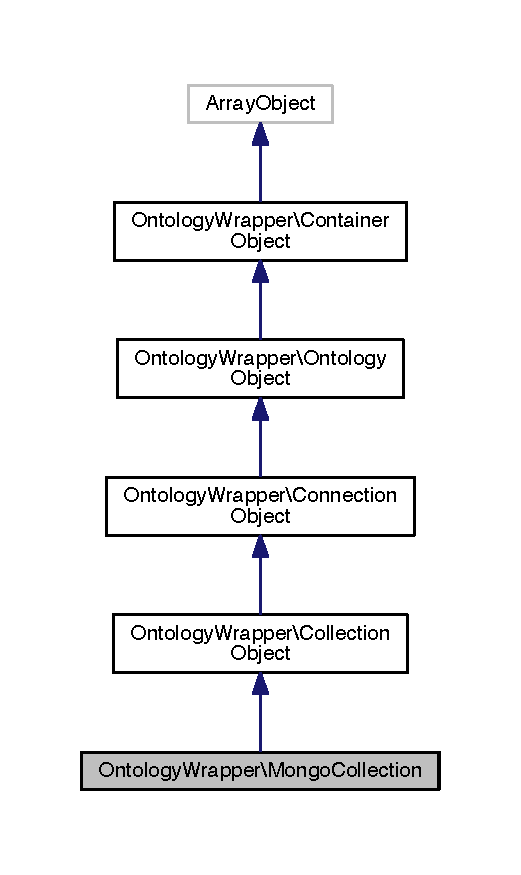
\includegraphics[width=250pt]{class_ontology_wrapper_1_1_mongo_collection__inherit__graph}
\end{center}
\end{figure}


Collaboration diagram for Ontology\-Wrapper\textbackslash{}Mongo\-Collection\-:\nopagebreak
\begin{figure}[H]
\begin{center}
\leavevmode
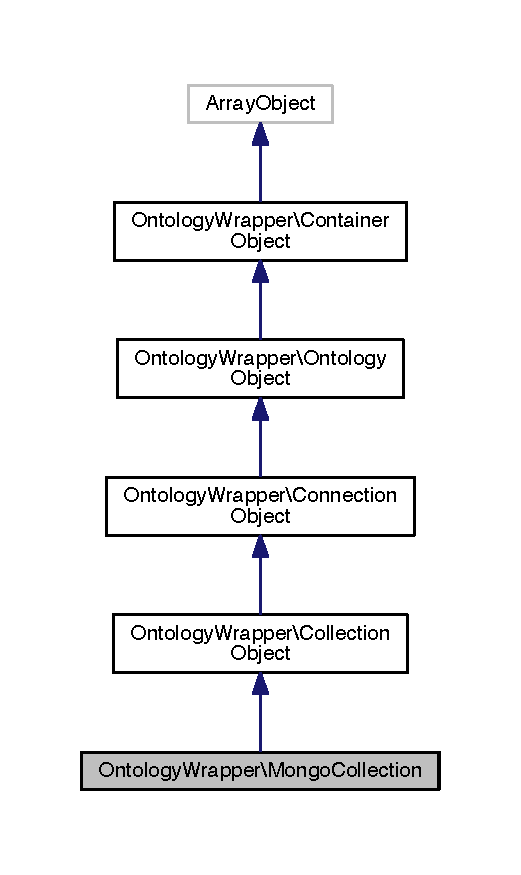
\includegraphics[width=250pt]{class_ontology_wrapper_1_1_mongo_collection__coll__graph}
\end{center}
\end{figure}
\subsection*{Public Member Functions}
\begin{DoxyCompactItemize}
\item 
\hyperlink{class_ontology_wrapper_1_1_mongo_collection_aeee231e29de0e8767d85164a7e833c44}{drop} ()
\item 
\hyperlink{class_ontology_wrapper_1_1_mongo_collection_a560202c9b4f73c72f0ed80729308aa58}{is\-Connected} ()
\item 
\hyperlink{class_ontology_wrapper_1_1_mongo_collection_a60a5da13657f31f20ca01561d21404f4}{resolve} (\$the\-Identifier, \$the\-Offset=k\-T\-A\-G\-\_\-\-N\-I\-D, \$as\-Object=T\-R\-U\-E)
\item 
\hyperlink{class_ontology_wrapper_1_1_mongo_collection_a230bf677670eb7f19cd8a01d15f96d15}{get\-All} ()
\item 
\hyperlink{class_ontology_wrapper_1_1_mongo_collection_aea1c5282361f10158efbb23319e53d03}{insert\-Data} (\&\$the\-Data, \&\$the\-Options)
\end{DoxyCompactItemize}
\subsection*{Protected Member Functions}
\begin{DoxyCompactItemize}
\item 
\hyperlink{class_ontology_wrapper_1_1_mongo_collection_a92cf5edd7c20d32dfe51e516ac4e6324}{connection\-Open} ()
\item 
\hyperlink{class_ontology_wrapper_1_1_mongo_collection_a7e9e367c57fc693f2ee83bb4ccfd7c27}{connection\-Close} ()
\item 
\hyperlink{class_ontology_wrapper_1_1_mongo_collection_a930abfb62b02f4dee7fad461f8edbbc3}{new\-Database} (\$the\-Parameter, \$do\-Open=T\-R\-U\-E)
\end{DoxyCompactItemize}
\subsection*{Additional Inherited Members}


\subsection{Detailed Description}
Mongo database

This class is a {\itshape concrete} implementation of the \hyperlink{class_ontology_wrapper_1_1_collection_object}{Collection\-Object} wrapping a \hyperlink{}{Mongo\-D\-B} class. \begin{DoxyVerb} @author            Milko A. Škofič <m.skofic@cgiar.org>
 @version   1.00 07/02/2014\end{DoxyVerb}
 

\subsection{Member Function Documentation}
\hypertarget{class_ontology_wrapper_1_1_mongo_collection_a7e9e367c57fc693f2ee83bb4ccfd7c27}{\index{Ontology\-Wrapper\-::\-Mongo\-Collection@{Ontology\-Wrapper\-::\-Mongo\-Collection}!connection\-Close@{connection\-Close}}
\index{connection\-Close@{connection\-Close}!OntologyWrapper::MongoCollection@{Ontology\-Wrapper\-::\-Mongo\-Collection}}
\subsubsection[{connection\-Close}]{\setlength{\rightskip}{0pt plus 5cm}Ontology\-Wrapper\textbackslash{}\-Mongo\-Collection\-::connection\-Close (
\begin{DoxyParamCaption}
{}
\end{DoxyParamCaption}
)\hspace{0.3cm}{\ttfamily [protected]}}}\label{class_ontology_wrapper_1_1_mongo_collection_a7e9e367c57fc693f2ee83bb4ccfd7c27}
Close connection

We overload this method to reset the connection resource.

protected \hypertarget{class_ontology_wrapper_1_1_mongo_collection_a92cf5edd7c20d32dfe51e516ac4e6324}{\index{Ontology\-Wrapper\-::\-Mongo\-Collection@{Ontology\-Wrapper\-::\-Mongo\-Collection}!connection\-Open@{connection\-Open}}
\index{connection\-Open@{connection\-Open}!OntologyWrapper::MongoCollection@{Ontology\-Wrapper\-::\-Mongo\-Collection}}
\subsubsection[{connection\-Open}]{\setlength{\rightskip}{0pt plus 5cm}Ontology\-Wrapper\textbackslash{}\-Mongo\-Collection\-::connection\-Open (
\begin{DoxyParamCaption}
{}
\end{DoxyParamCaption}
)\hspace{0.3cm}{\ttfamily [protected]}}}\label{class_ontology_wrapper_1_1_mongo_collection_a92cf5edd7c20d32dfe51e516ac4e6324}
Open connection

This method will instantiate a Mongo\-Collectionobjectandsetitinthe@linkConnection()datamember.Thismethodexpectsthecallertohavecheckedwhethertheconnectionisalreadyopen.Iftheoperationfails,themethodwillraiseanexception.@accessprotected@returnmixedThenativeconnection.@throwsException\hypertarget{class_ontology_wrapper_1_1_mongo_collection_aeee231e29de0e8767d85164a7e833c44}{\index{Ontology\-Wrapper\-::\-Mongo\-Collection@{Ontology\-Wrapper\-::\-Mongo\-Collection}!drop@{drop}}
\index{drop@{drop}!OntologyWrapper::MongoCollection@{Ontology\-Wrapper\-::\-Mongo\-Collection}}
\subsubsection[{drop}]{\setlength{\rightskip}{0pt plus 5cm}Ontology\-Wrapper\textbackslash{}\-Mongo\-Collection\-::drop (
\begin{DoxyParamCaption}
{}
\end{DoxyParamCaption}
)}}\label{class_ontology_wrapper_1_1_mongo_collection_aeee231e29de0e8767d85164a7e833c44}
Drop the database

This method will drop the current collection.

public


\begin{DoxyExceptions}{Exceptions}
{\em Exception} & \\
\hline
\end{DoxyExceptions}
\hypertarget{class_ontology_wrapper_1_1_mongo_collection_a230bf677670eb7f19cd8a01d15f96d15}{\index{Ontology\-Wrapper\-::\-Mongo\-Collection@{Ontology\-Wrapper\-::\-Mongo\-Collection}!get\-All@{get\-All}}
\index{get\-All@{get\-All}!OntologyWrapper::MongoCollection@{Ontology\-Wrapper\-::\-Mongo\-Collection}}
\subsubsection[{get\-All}]{\setlength{\rightskip}{0pt plus 5cm}Ontology\-Wrapper\textbackslash{}\-Mongo\-Collection\-::get\-All (
\begin{DoxyParamCaption}
{}
\end{DoxyParamCaption}
)}}\label{class_ontology_wrapper_1_1_mongo_collection_a230bf677670eb7f19cd8a01d15f96d15}
Return all objects

In this class we return a \hyperlink{}{Mongo\-Cursor} object.

public \begin{DoxyReturn}{Returns}
Iterator Selection of all objects of the collection.
\end{DoxyReturn}

\begin{DoxyExceptions}{Exceptions}
{\em Exception} & \\
\hline
\end{DoxyExceptions}
\hypertarget{class_ontology_wrapper_1_1_mongo_collection_aea1c5282361f10158efbb23319e53d03}{\index{Ontology\-Wrapper\-::\-Mongo\-Collection@{Ontology\-Wrapper\-::\-Mongo\-Collection}!insert\-Data@{insert\-Data}}
\index{insert\-Data@{insert\-Data}!OntologyWrapper::MongoCollection@{Ontology\-Wrapper\-::\-Mongo\-Collection}}
\subsubsection[{insert\-Data}]{\setlength{\rightskip}{0pt plus 5cm}Ontology\-Wrapper\textbackslash{}\-Mongo\-Collection\-::insert\-Data (
\begin{DoxyParamCaption}
\item[{\&}]{\$the\-Data, }
\item[{\&}]{\$the\-Options}
\end{DoxyParamCaption}
)}}\label{class_ontology_wrapper_1_1_mongo_collection_aea1c5282361f10158efbb23319e53d03}
Insert provided data

In this class we commit the provided array and return its \hyperlink{}{k\-T\-A\-G\-\_\-\-N\-I\-D} value.


\begin{DoxyParams}[1]{Parameters}
reference & {\em \$the\-Data} & Data to commit. \\
\hline
array & {\em \$the\-Options} & Insert options.\\
\hline
\end{DoxyParams}
protected \begin{DoxyReturn}{Returns}
mixed Object identifier. 
\end{DoxyReturn}
\hypertarget{class_ontology_wrapper_1_1_mongo_collection_a560202c9b4f73c72f0ed80729308aa58}{\index{Ontology\-Wrapper\-::\-Mongo\-Collection@{Ontology\-Wrapper\-::\-Mongo\-Collection}!is\-Connected@{is\-Connected}}
\index{is\-Connected@{is\-Connected}!OntologyWrapper::MongoCollection@{Ontology\-Wrapper\-::\-Mongo\-Collection}}
\subsubsection[{is\-Connected}]{\setlength{\rightskip}{0pt plus 5cm}Ontology\-Wrapper\textbackslash{}\-Mongo\-Collection\-::is\-Connected (
\begin{DoxyParamCaption}
{}
\end{DoxyParamCaption}
)}}\label{class_ontology_wrapper_1_1_mongo_collection_a560202c9b4f73c72f0ed80729308aa58}
Check if connection is open

We overload this method to assume the object is connected if the resource is a \hyperlink{}{Mongo\-D\-B}.

public \begin{DoxyReturn}{Returns}
boolean {\ttfamily T\-R\-U\-E} is open. 
\end{DoxyReturn}
\hypertarget{class_ontology_wrapper_1_1_mongo_collection_a930abfb62b02f4dee7fad461f8edbbc3}{\index{Ontology\-Wrapper\-::\-Mongo\-Collection@{Ontology\-Wrapper\-::\-Mongo\-Collection}!new\-Database@{new\-Database}}
\index{new\-Database@{new\-Database}!OntologyWrapper::MongoCollection@{Ontology\-Wrapper\-::\-Mongo\-Collection}}
\subsubsection[{new\-Database}]{\setlength{\rightskip}{0pt plus 5cm}Ontology\-Wrapper\textbackslash{}\-Mongo\-Collection\-::new\-Database (
\begin{DoxyParamCaption}
\item[{}]{\$the\-Parameter, }
\item[{}]{\$do\-Open = {\ttfamily TRUE}}
\end{DoxyParamCaption}
)\hspace{0.3cm}{\ttfamily [protected]}}}\label{class_ontology_wrapper_1_1_mongo_collection_a930abfb62b02f4dee7fad461f8edbbc3}
Return a new database instance

We implement the method to return a \hyperlink{class_ontology_wrapper_1_1_mongo_server}{Mongo\-Server} instance.


\begin{DoxyParams}[1]{Parameters}
mixed & {\em \$the\-Parameter} & Server parameters. \\
\hline
boolean & {\em \$do\-Open} & {\ttfamily T\-R\-U\-E} open connection.\\
\hline
\end{DoxyParams}
protected \begin{DoxyReturn}{Returns}
\hyperlink{class_ontology_wrapper_1_1_database_object}{Database\-Object} Database instance. 
\end{DoxyReturn}
\hypertarget{class_ontology_wrapper_1_1_mongo_collection_a60a5da13657f31f20ca01561d21404f4}{\index{Ontology\-Wrapper\-::\-Mongo\-Collection@{Ontology\-Wrapper\-::\-Mongo\-Collection}!resolve@{resolve}}
\index{resolve@{resolve}!OntologyWrapper::MongoCollection@{Ontology\-Wrapper\-::\-Mongo\-Collection}}
\subsubsection[{resolve}]{\setlength{\rightskip}{0pt plus 5cm}Ontology\-Wrapper\textbackslash{}\-Mongo\-Collection\-::resolve (
\begin{DoxyParamCaption}
\item[{}]{\$the\-Identifier, }
\item[{}]{\$the\-Offset = {\ttfamily kTAG\-\_\-NID}, }
\item[{}]{\$as\-Object = {\ttfamily TRUE}}
\end{DoxyParamCaption}
)}}\label{class_ontology_wrapper_1_1_mongo_collection_a60a5da13657f31f20ca01561d21404f4}
Resolve an identifier

We first check if the current collection is connected, if that is not the case, we raise an exception.


\begin{DoxyParams}[1]{Parameters}
mixed & {\em \$the\-Identifier} & Object identifier. \\
\hline
mixed & {\em \$the\-Offset} & Offset. \\
\hline
mixed & {\em \$as\-Object} & Return object if {\ttfamily T\-R\-U\-E}.\\
\hline
\end{DoxyParams}
public \begin{DoxyReturn}{Returns}
mixed Found object, array, objects count or {\ttfamily N\-U\-L\-L}.
\end{DoxyReturn}

\begin{DoxyExceptions}{Exceptions}
{\em Exception} & \\
\hline
\end{DoxyExceptions}


The documentation for this class was generated from the following file\-:\begin{DoxyCompactItemize}
\item 
/\-Library/\-Web\-Server/\-Library/\-Ontology\-Wrapper/\-Library/\-Ontology\-Wrapper/Mongo\-Collection.\-php\end{DoxyCompactItemize}

\hypertarget{class_ontology_wrapper_1_1_mongo_database}{\section{Ontology\-Wrapper\textbackslash{}Mongo\-Database Class Reference}
\label{class_ontology_wrapper_1_1_mongo_database}\index{Ontology\-Wrapper\textbackslash{}\-Mongo\-Database@{Ontology\-Wrapper\textbackslash{}\-Mongo\-Database}}
}


Inheritance diagram for Ontology\-Wrapper\textbackslash{}Mongo\-Database\-:\nopagebreak
\begin{figure}[H]
\begin{center}
\leavevmode
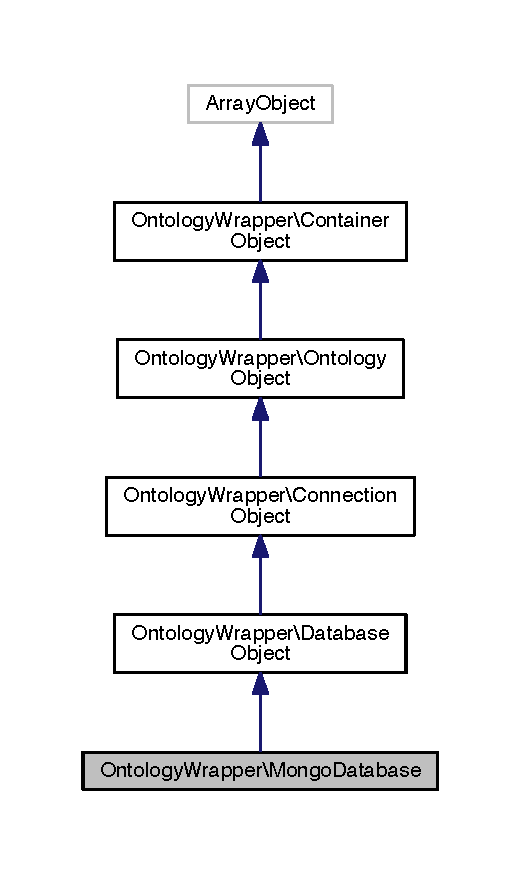
\includegraphics[width=250pt]{class_ontology_wrapper_1_1_mongo_database__inherit__graph}
\end{center}
\end{figure}


Collaboration diagram for Ontology\-Wrapper\textbackslash{}Mongo\-Database\-:\nopagebreak
\begin{figure}[H]
\begin{center}
\leavevmode
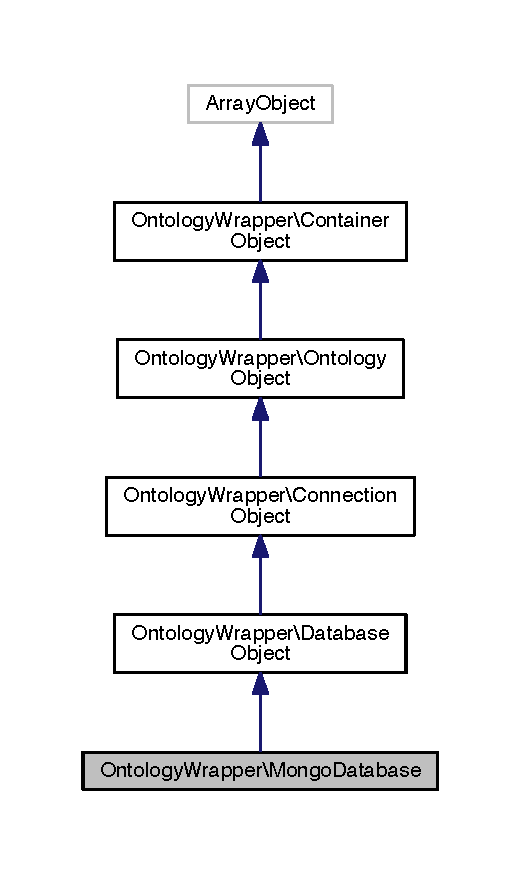
\includegraphics[width=250pt]{class_ontology_wrapper_1_1_mongo_database__coll__graph}
\end{center}
\end{figure}
\subsection*{Public Member Functions}
\begin{DoxyCompactItemize}
\item 
\hyperlink{class_ontology_wrapper_1_1_mongo_database_ab3df5cac7ce7f15f3c3a2c0feb9cb0ae}{drop} ()
\item 
\hyperlink{class_ontology_wrapper_1_1_mongo_database_aa0d740a0f02a9093b84367d608e0b781}{is\-Connected} ()
\item 
\hyperlink{class_ontology_wrapper_1_1_mongo_database_aea2876ae9fc23f227d34fadfcd91c52b}{get\-Collections} ()
\item 
\hyperlink{class_ontology_wrapper_1_1_mongo_database_abb8850dbf55ad8684ec5244f60d220ba}{set\-Sequence\-Number} (\$the\-Sequence, \$the\-Number=1)
\item 
\hyperlink{class_ontology_wrapper_1_1_mongo_database_a86848d0cc3c72a0a40938338483799a7}{get\-Sequence\-Number} (\$the\-Sequence)
\end{DoxyCompactItemize}
\subsection*{Public Attributes}
\begin{DoxyCompactItemize}
\item 
\hypertarget{class_ontology_wrapper_1_1_mongo_database_a3d737abcfa3f477fa6b90fcd44cf6952}{const {\bfseries k\-S\-E\-Q\-\_\-\-C\-O\-L\-L\-E\-C\-T\-I\-O\-N} = '\-\_\-sequence'}\label{class_ontology_wrapper_1_1_mongo_database_a3d737abcfa3f477fa6b90fcd44cf6952}

\item 
\hypertarget{class_ontology_wrapper_1_1_mongo_database_a267f9e486b60ce3d63b67c2f215be9f2}{const {\bfseries k\-S\-E\-Q\-\_\-\-O\-F\-F\-S\-E\-T} = '\-\_\-seq'}\label{class_ontology_wrapper_1_1_mongo_database_a267f9e486b60ce3d63b67c2f215be9f2}

\end{DoxyCompactItemize}
\subsection*{Protected Member Functions}
\begin{DoxyCompactItemize}
\item 
\hyperlink{class_ontology_wrapper_1_1_mongo_database_a4b976e0857cbbbfd1fba2b33b7b2512c}{connection\-Open} ()
\item 
\hyperlink{class_ontology_wrapper_1_1_mongo_database_a0960889565708ebe8759388284043d6d}{connection\-Close} ()
\item 
\hyperlink{class_ontology_wrapper_1_1_mongo_database_ac3a49cd81d3ac17aa707258b6758b07c}{new\-Server} (\$the\-Parameter, \$do\-Open=T\-R\-U\-E)
\item 
\hyperlink{class_ontology_wrapper_1_1_mongo_database_a8e68fc8ae64675dffa862fcff79dea4b}{new\-Collection} (\$the\-Offsets, \$do\-Open=T\-R\-U\-E)
\end{DoxyCompactItemize}
\subsection*{Additional Inherited Members}


\subsection{Detailed Description}
Mongo database

This class is a {\itshape concrete} implementation of the \hyperlink{class_ontology_wrapper_1_1_database_object}{Database\-Object} wrapping a \hyperlink{}{Mongo\-D\-B} class. \begin{DoxyVerb} @author            Milko A. Škofič <m.skofic@cgiar.org>
 @version   1.00 06/02/2014\end{DoxyVerb}
 

\subsection{Member Function Documentation}
\hypertarget{class_ontology_wrapper_1_1_mongo_database_a0960889565708ebe8759388284043d6d}{\index{Ontology\-Wrapper\-::\-Mongo\-Database@{Ontology\-Wrapper\-::\-Mongo\-Database}!connection\-Close@{connection\-Close}}
\index{connection\-Close@{connection\-Close}!OntologyWrapper::MongoDatabase@{Ontology\-Wrapper\-::\-Mongo\-Database}}
\subsubsection[{connection\-Close}]{\setlength{\rightskip}{0pt plus 5cm}Ontology\-Wrapper\textbackslash{}\-Mongo\-Database\-::connection\-Close (
\begin{DoxyParamCaption}
{}
\end{DoxyParamCaption}
)\hspace{0.3cm}{\ttfamily [protected]}}}\label{class_ontology_wrapper_1_1_mongo_database_a0960889565708ebe8759388284043d6d}
Close connection

We overload this method to reset the connection resource.

protected \hypertarget{class_ontology_wrapper_1_1_mongo_database_a4b976e0857cbbbfd1fba2b33b7b2512c}{\index{Ontology\-Wrapper\-::\-Mongo\-Database@{Ontology\-Wrapper\-::\-Mongo\-Database}!connection\-Open@{connection\-Open}}
\index{connection\-Open@{connection\-Open}!OntologyWrapper::MongoDatabase@{Ontology\-Wrapper\-::\-Mongo\-Database}}
\subsubsection[{connection\-Open}]{\setlength{\rightskip}{0pt plus 5cm}Ontology\-Wrapper\textbackslash{}\-Mongo\-Database\-::connection\-Open (
\begin{DoxyParamCaption}
{}
\end{DoxyParamCaption}
)\hspace{0.3cm}{\ttfamily [protected]}}}\label{class_ontology_wrapper_1_1_mongo_database_a4b976e0857cbbbfd1fba2b33b7b2512c}
Open connection

This method will instantiate a \hyperlink{}{Mongo\-D\-B} object and set it in the \hyperlink{class_ontology_wrapper_1_1_connection_object_aeffe3ba284ae71caacaab38b3c80d345}{Connection()} data member.

This method expects the caller to have checked whether the connection is already open.

If the operation fails, the method will raise an exception.

protected \begin{DoxyReturn}{Returns}
mixed The native connection.
\end{DoxyReturn}

\begin{DoxyExceptions}{Exceptions}
{\em Exception} & \\
\hline
\end{DoxyExceptions}
\hypertarget{class_ontology_wrapper_1_1_mongo_database_ab3df5cac7ce7f15f3c3a2c0feb9cb0ae}{\index{Ontology\-Wrapper\-::\-Mongo\-Database@{Ontology\-Wrapper\-::\-Mongo\-Database}!drop@{drop}}
\index{drop@{drop}!OntologyWrapper::MongoDatabase@{Ontology\-Wrapper\-::\-Mongo\-Database}}
\subsubsection[{drop}]{\setlength{\rightskip}{0pt plus 5cm}Ontology\-Wrapper\textbackslash{}\-Mongo\-Database\-::drop (
\begin{DoxyParamCaption}
{}
\end{DoxyParamCaption}
)}}\label{class_ontology_wrapper_1_1_mongo_database_ab3df5cac7ce7f15f3c3a2c0feb9cb0ae}
Drop the database

This method will drop the current database.

public


\begin{DoxyExceptions}{Exceptions}
{\em Exception} & \\
\hline
\end{DoxyExceptions}
\hypertarget{class_ontology_wrapper_1_1_mongo_database_aea2876ae9fc23f227d34fadfcd91c52b}{\index{Ontology\-Wrapper\-::\-Mongo\-Database@{Ontology\-Wrapper\-::\-Mongo\-Database}!get\-Collections@{get\-Collections}}
\index{get\-Collections@{get\-Collections}!OntologyWrapper::MongoDatabase@{Ontology\-Wrapper\-::\-Mongo\-Database}}
\subsubsection[{get\-Collections}]{\setlength{\rightskip}{0pt plus 5cm}Ontology\-Wrapper\textbackslash{}\-Mongo\-Database\-::get\-Collections (
\begin{DoxyParamCaption}
{}
\end{DoxyParamCaption}
)}}\label{class_ontology_wrapper_1_1_mongo_database_aea2876ae9fc23f227d34fadfcd91c52b}
Return collection names

In this class we use the Mongo\-D\-B\-::list\-Collections()method,weextractonlythenametoconformwiththemethodprototype\-:oneshouldalwaysinstantiateanobjectderivedfrom@linkCollection\-Objectwhendealingwitcollections.Thismethodwillreturnthefollowingretults\-:$<$ul$>$$<$li$>$$<$tt$>$\-F\-A\-L\-S\-E$<$/tt$>$\-:Thedatabaseisnotconnected.$<$li$>$$<$tt$>$array$<$/tt$>$\-:Thedatabasecollectionnames.$<$/ul$>$@accesspublic@returnarrayListofcollectionnames.\hypertarget{class_ontology_wrapper_1_1_mongo_database_a86848d0cc3c72a0a40938338483799a7}{\index{Ontology\-Wrapper\-::\-Mongo\-Database@{Ontology\-Wrapper\-::\-Mongo\-Database}!get\-Sequence\-Number@{get\-Sequence\-Number}}
\index{get\-Sequence\-Number@{get\-Sequence\-Number}!OntologyWrapper::MongoDatabase@{Ontology\-Wrapper\-::\-Mongo\-Database}}
\subsubsection[{get\-Sequence\-Number}]{\setlength{\rightskip}{0pt plus 5cm}Ontology\-Wrapper\textbackslash{}\-Mongo\-Database\-::get\-Sequence\-Number (
\begin{DoxyParamCaption}
\item[{}]{\$the\-Sequence}
\end{DoxyParamCaption}
)}}\label{class_ontology_wrapper_1_1_mongo_database_a86848d0cc3c72a0a40938338483799a7}
Return sequence number

In this class we match the provided parameter string with an entry in the \hyperlink{}{k\-S\-E\-Q\-\_\-\-C\-O\-L\-L\-E\-C\-T\-I\-O\-N} collection in the database, the native identifier of the record is the sequence selector, while the sequence number will be found at the \hyperlink{}{k\-S\-E\-Q\-\_\-\-O\-F\-F\-S\-E\-T} offset.


\begin{DoxyParams}[1]{Parameters}
string & {\em \$the\-Sequence} & Sequence selector.\\
\hline
\end{DoxyParams}
public \begin{DoxyReturn}{Returns}
integer Sequence number.
\end{DoxyReturn}

\begin{DoxyExceptions}{Exceptions}
{\em Exception} & \\
\hline
\end{DoxyExceptions}
\hypertarget{class_ontology_wrapper_1_1_mongo_database_aa0d740a0f02a9093b84367d608e0b781}{\index{Ontology\-Wrapper\-::\-Mongo\-Database@{Ontology\-Wrapper\-::\-Mongo\-Database}!is\-Connected@{is\-Connected}}
\index{is\-Connected@{is\-Connected}!OntologyWrapper::MongoDatabase@{Ontology\-Wrapper\-::\-Mongo\-Database}}
\subsubsection[{is\-Connected}]{\setlength{\rightskip}{0pt plus 5cm}Ontology\-Wrapper\textbackslash{}\-Mongo\-Database\-::is\-Connected (
\begin{DoxyParamCaption}
{}
\end{DoxyParamCaption}
)}}\label{class_ontology_wrapper_1_1_mongo_database_aa0d740a0f02a9093b84367d608e0b781}
Check if connection is open

We overload this method to assume the object is connected if the resource is a \hyperlink{}{Mongo\-D\-B}.

public \begin{DoxyReturn}{Returns}
boolean {\ttfamily T\-R\-U\-E} is open. 
\end{DoxyReturn}
\hypertarget{class_ontology_wrapper_1_1_mongo_database_a8e68fc8ae64675dffa862fcff79dea4b}{\index{Ontology\-Wrapper\-::\-Mongo\-Database@{Ontology\-Wrapper\-::\-Mongo\-Database}!new\-Collection@{new\-Collection}}
\index{new\-Collection@{new\-Collection}!OntologyWrapper::MongoDatabase@{Ontology\-Wrapper\-::\-Mongo\-Database}}
\subsubsection[{new\-Collection}]{\setlength{\rightskip}{0pt plus 5cm}Ontology\-Wrapper\textbackslash{}\-Mongo\-Database\-::new\-Collection (
\begin{DoxyParamCaption}
\item[{}]{\$the\-Offsets, }
\item[{}]{\$do\-Open = {\ttfamily TRUE}}
\end{DoxyParamCaption}
)\hspace{0.3cm}{\ttfamily [protected]}}}\label{class_ontology_wrapper_1_1_mongo_database_a8e68fc8ae64675dffa862fcff79dea4b}
Return a new collection instance

We implement this method to return a \hyperlink{class_ontology_wrapper_1_1_mongo_collection}{Mongo\-Collection} instance.


\begin{DoxyParams}[1]{Parameters}
array & {\em \$the\-Offsets} & Full collection offsets. \\
\hline
boolean & {\em \$do\-Open} & {\ttfamily T\-R\-U\-E} open connection.\\
\hline
\end{DoxyParams}
protected \begin{DoxyReturn}{Returns}
\hyperlink{class_ontology_wrapper_1_1_collection_object}{Collection\-Object} Collection instance. 
\end{DoxyReturn}
\hypertarget{class_ontology_wrapper_1_1_mongo_database_ac3a49cd81d3ac17aa707258b6758b07c}{\index{Ontology\-Wrapper\-::\-Mongo\-Database@{Ontology\-Wrapper\-::\-Mongo\-Database}!new\-Server@{new\-Server}}
\index{new\-Server@{new\-Server}!OntologyWrapper::MongoDatabase@{Ontology\-Wrapper\-::\-Mongo\-Database}}
\subsubsection[{new\-Server}]{\setlength{\rightskip}{0pt plus 5cm}Ontology\-Wrapper\textbackslash{}\-Mongo\-Database\-::new\-Server (
\begin{DoxyParamCaption}
\item[{}]{\$the\-Parameter, }
\item[{}]{\$do\-Open = {\ttfamily TRUE}}
\end{DoxyParamCaption}
)\hspace{0.3cm}{\ttfamily [protected]}}}\label{class_ontology_wrapper_1_1_mongo_database_ac3a49cd81d3ac17aa707258b6758b07c}
Return a new server instance

We implement the method to return a \hyperlink{class_ontology_wrapper_1_1_mongo_server}{Mongo\-Server} instance and set the current object dictionary in it.


\begin{DoxyParams}[1]{Parameters}
mixed & {\em \$the\-Parameter} & Server parameters. \\
\hline
boolean & {\em \$do\-Open} & {\ttfamily T\-R\-U\-E} open connection.\\
\hline
\end{DoxyParams}
protected \begin{DoxyReturn}{Returns}
\hyperlink{class_ontology_wrapper_1_1_mongo_server}{Mongo\-Server} Server instance. 
\end{DoxyReturn}
\hypertarget{class_ontology_wrapper_1_1_mongo_database_abb8850dbf55ad8684ec5244f60d220ba}{\index{Ontology\-Wrapper\-::\-Mongo\-Database@{Ontology\-Wrapper\-::\-Mongo\-Database}!set\-Sequence\-Number@{set\-Sequence\-Number}}
\index{set\-Sequence\-Number@{set\-Sequence\-Number}!OntologyWrapper::MongoDatabase@{Ontology\-Wrapper\-::\-Mongo\-Database}}
\subsubsection[{set\-Sequence\-Number}]{\setlength{\rightskip}{0pt plus 5cm}Ontology\-Wrapper\textbackslash{}\-Mongo\-Database\-::set\-Sequence\-Number (
\begin{DoxyParamCaption}
\item[{}]{\$the\-Sequence, }
\item[{}]{\$the\-Number = {\ttfamily 1}}
\end{DoxyParamCaption}
)}}\label{class_ontology_wrapper_1_1_mongo_database_abb8850dbf55ad8684ec5244f60d220ba}
Set sequence number

In this class we match the provided parameter string with an entry in the \hyperlink{}{k\-S\-E\-Q\-\_\-\-C\-O\-L\-L\-E\-C\-T\-I\-O\-N} collection in the database, the native identifier of the record is the sequence selector, while the sequence number will be found at the \hyperlink{}{k\-S\-E\-Q\-\_\-\-O\-F\-F\-S\-E\-T} offset.


\begin{DoxyParams}[1]{Parameters}
string & {\em \$the\-Sequence} & Sequence selector. \\
\hline
integer & {\em \$the\-Number} & Sequence number.\\
\hline
\end{DoxyParams}
public


\begin{DoxyExceptions}{Exceptions}
{\em Exception} & \\
\hline
\end{DoxyExceptions}


The documentation for this class was generated from the following file\-:\begin{DoxyCompactItemize}
\item 
/\-Library/\-Web\-Server/\-Library/\-Ontology\-Wrapper/\-Library/\-Ontology\-Wrapper/Mongo\-Database.\-php\end{DoxyCompactItemize}

\hypertarget{class_ontology_wrapper_1_1_mongo_server}{\section{Ontology\-Wrapper\textbackslash{}Mongo\-Server Class Reference}
\label{class_ontology_wrapper_1_1_mongo_server}\index{Ontology\-Wrapper\textbackslash{}\-Mongo\-Server@{Ontology\-Wrapper\textbackslash{}\-Mongo\-Server}}
}


Inheritance diagram for Ontology\-Wrapper\textbackslash{}Mongo\-Server\-:
\nopagebreak
\begin{figure}[H]
\begin{center}
\leavevmode
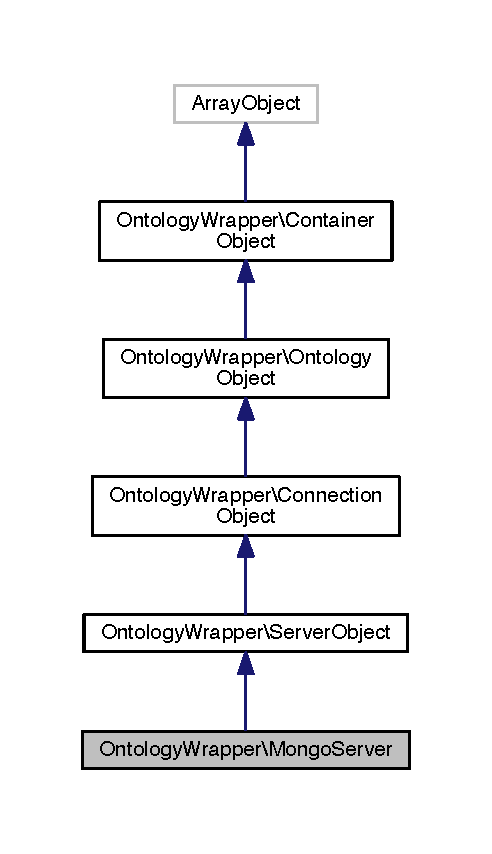
\includegraphics[width=236pt]{class_ontology_wrapper_1_1_mongo_server__inherit__graph}
\end{center}
\end{figure}


Collaboration diagram for Ontology\-Wrapper\textbackslash{}Mongo\-Server\-:
\nopagebreak
\begin{figure}[H]
\begin{center}
\leavevmode
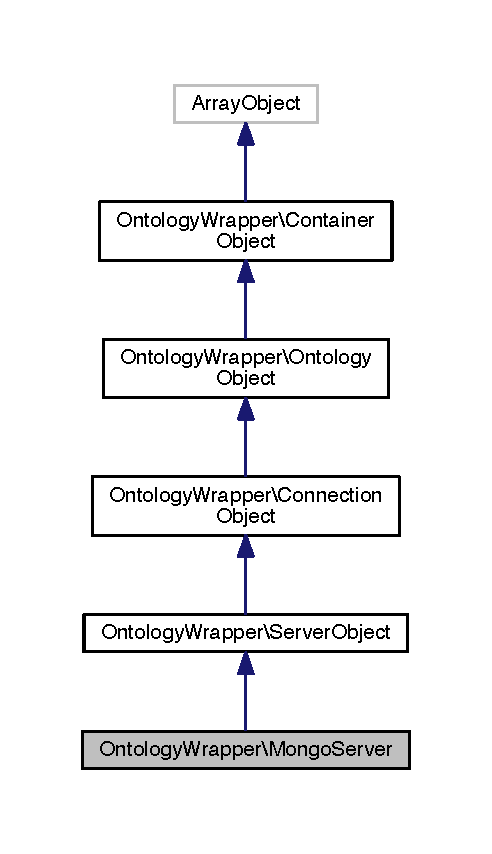
\includegraphics[width=236pt]{class_ontology_wrapper_1_1_mongo_server__coll__graph}
\end{center}
\end{figure}
\subsection*{Public Member Functions}
\begin{DoxyCompactItemize}
\item 
\hyperlink{class_ontology_wrapper_1_1_mongo_server_a2bde1d3f28624801cbb42bf8b94673d4}{is\-Connected} ()
\item 
\hyperlink{class_ontology_wrapper_1_1_mongo_server_ad0339362ebaba5c344a179ef11d4e102}{get\-Statistics} ()
\end{DoxyCompactItemize}
\subsection*{Protected Member Functions}
\begin{DoxyCompactItemize}
\item 
\hyperlink{class_ontology_wrapper_1_1_mongo_server_abd478e3c641bbe1f40f7edf41e986558}{connection\-Open} ()
\item 
\hyperlink{class_ontology_wrapper_1_1_mongo_server_a0817afd4db82e176e0ebb6c7d5752e6e}{connection\-Close} ()
\item 
\hyperlink{class_ontology_wrapper_1_1_mongo_server_a511427a098b640515401bbb6baba7515}{new\-Database} (\$the\-Offsets)
\end{DoxyCompactItemize}
\subsection*{Additional Inherited Members}


\subsection{Detailed Description}
Mongo server

This class is a {\itshape concrete} implementation of the \hyperlink{class_ontology_wrapper_1_1_server_object}{Server\-Object} wrapping a \hyperlink{}{Mongo\-Client} class. \begin{DoxyVerb} @author            Milko A. Škofič <m.skofic@cgiar.org>
 @version   1.00 06/02/2014\end{DoxyVerb}
 

\subsection{Member Function Documentation}
\hypertarget{class_ontology_wrapper_1_1_mongo_server_a0817afd4db82e176e0ebb6c7d5752e6e}{\index{Ontology\-Wrapper\-::\-Mongo\-Server@{Ontology\-Wrapper\-::\-Mongo\-Server}!connection\-Close@{connection\-Close}}
\index{connection\-Close@{connection\-Close}!OntologyWrapper::MongoServer@{Ontology\-Wrapper\-::\-Mongo\-Server}}
\subsubsection[{connection\-Close}]{\setlength{\rightskip}{0pt plus 5cm}Ontology\-Wrapper\textbackslash{}\-Mongo\-Server\-::connection\-Close (
\begin{DoxyParamCaption}
{}
\end{DoxyParamCaption}
)\hspace{0.3cm}{\ttfamily [protected]}}}\label{class_ontology_wrapper_1_1_mongo_server_a0817afd4db82e176e0ebb6c7d5752e6e}
Close connection

We overload this method to reset the connection resource.

protected \hypertarget{class_ontology_wrapper_1_1_mongo_server_abd478e3c641bbe1f40f7edf41e986558}{\index{Ontology\-Wrapper\-::\-Mongo\-Server@{Ontology\-Wrapper\-::\-Mongo\-Server}!connection\-Open@{connection\-Open}}
\index{connection\-Open@{connection\-Open}!OntologyWrapper::MongoServer@{Ontology\-Wrapper\-::\-Mongo\-Server}}
\subsubsection[{connection\-Open}]{\setlength{\rightskip}{0pt plus 5cm}Ontology\-Wrapper\textbackslash{}\-Mongo\-Server\-::connection\-Open (
\begin{DoxyParamCaption}
{}
\end{DoxyParamCaption}
)\hspace{0.3cm}{\ttfamily [protected]}}}\label{class_ontology_wrapper_1_1_mongo_server_abd478e3c641bbe1f40f7edf41e986558}
Open connection

This method will instantiate a \hyperlink{}{Mongo\-Client} object and set it in the m\-Connection data member.

This method expects the caller to have checked whether the connection is already open.

If the operation fails, the method will raise an exception.

protected \begin{DoxyReturn}{Returns}
mixed The native connection. 
\end{DoxyReturn}
\hypertarget{class_ontology_wrapper_1_1_mongo_server_ad0339362ebaba5c344a179ef11d4e102}{\index{Ontology\-Wrapper\-::\-Mongo\-Server@{Ontology\-Wrapper\-::\-Mongo\-Server}!get\-Statistics@{get\-Statistics}}
\index{get\-Statistics@{get\-Statistics}!OntologyWrapper::MongoServer@{Ontology\-Wrapper\-::\-Mongo\-Server}}
\subsubsection[{get\-Statistics}]{\setlength{\rightskip}{0pt plus 5cm}Ontology\-Wrapper\textbackslash{}\-Mongo\-Server\-::get\-Statistics (
\begin{DoxyParamCaption}
{}
\end{DoxyParamCaption}
)}}\label{class_ontology_wrapper_1_1_mongo_server_ad0339362ebaba5c344a179ef11d4e102}
Return statistics

This method will return the following values\-:


\begin{DoxyItemize}
\item {\ttfamily F\-A\-L\-S\-E}\-: The server is not connected. 
\item {\ttfamily array}\-: The server statistics. 
\end{DoxyItemize}

public \begin{DoxyReturn}{Returns}
array Server statistics or {\ttfamily F\-A\-L\-S\-E}. 
\end{DoxyReturn}
\hypertarget{class_ontology_wrapper_1_1_mongo_server_a2bde1d3f28624801cbb42bf8b94673d4}{\index{Ontology\-Wrapper\-::\-Mongo\-Server@{Ontology\-Wrapper\-::\-Mongo\-Server}!is\-Connected@{is\-Connected}}
\index{is\-Connected@{is\-Connected}!OntologyWrapper::MongoServer@{Ontology\-Wrapper\-::\-Mongo\-Server}}
\subsubsection[{is\-Connected}]{\setlength{\rightskip}{0pt plus 5cm}Ontology\-Wrapper\textbackslash{}\-Mongo\-Server\-::is\-Connected (
\begin{DoxyParamCaption}
{}
\end{DoxyParamCaption}
)}}\label{class_ontology_wrapper_1_1_mongo_server_a2bde1d3f28624801cbb42bf8b94673d4}
Check if connection is open

We overload this method to assume the object is connected if the resource is a \hyperlink{}{Mongo\-Client}.

public \begin{DoxyReturn}{Returns}
boolean {\ttfamily T\-R\-U\-E} is open. 
\end{DoxyReturn}
\hypertarget{class_ontology_wrapper_1_1_mongo_server_a511427a098b640515401bbb6baba7515}{\index{Ontology\-Wrapper\-::\-Mongo\-Server@{Ontology\-Wrapper\-::\-Mongo\-Server}!new\-Database@{new\-Database}}
\index{new\-Database@{new\-Database}!OntologyWrapper::MongoServer@{Ontology\-Wrapper\-::\-Mongo\-Server}}
\subsubsection[{new\-Database}]{\setlength{\rightskip}{0pt plus 5cm}Ontology\-Wrapper\textbackslash{}\-Mongo\-Server\-::new\-Database (
\begin{DoxyParamCaption}
\item[{}]{\$the\-Offsets}
\end{DoxyParamCaption}
)\hspace{0.3cm}{\ttfamily [protected]}}}\label{class_ontology_wrapper_1_1_mongo_server_a511427a098b640515401bbb6baba7515}
Return a new database instance

This method should implemented by concrete derived classes, it expects a list of offsets which include server information and should use them to instantiate a \hyperlink{class_ontology_wrapper_1_1_database_object}{Database\-Object} instance.

Derived classes must implement this method.


\begin{DoxyParams}[1]{Parameters}
array & {\em \$the\-Offsets} & Full database offsets.\\
\hline
\end{DoxyParams}
protected \begin{DoxyReturn}{Returns}
\hyperlink{class_ontology_wrapper_1_1_database_object}{Database\-Object} Database instance. 
\end{DoxyReturn}


The documentation for this class was generated from the following file\-:\begin{DoxyCompactItemize}
\item 
/\-Library/\-Web\-Server/\-Library/\-Ontology\-Wrapper/\-Library/\-Ontology\-Wrapper/Mongo\-Server.\-php\end{DoxyCompactItemize}

\hypertarget{class_ontology_wrapper_1_1_node}{\section{Ontology\-Wrapper\textbackslash{}Node Class Reference}
\label{class_ontology_wrapper_1_1_node}\index{Ontology\-Wrapper\textbackslash{}\-Node@{Ontology\-Wrapper\textbackslash{}\-Node}}
}


Inheritance diagram for Ontology\-Wrapper\textbackslash{}Node\-:
\nopagebreak
\begin{figure}[H]
\begin{center}
\leavevmode
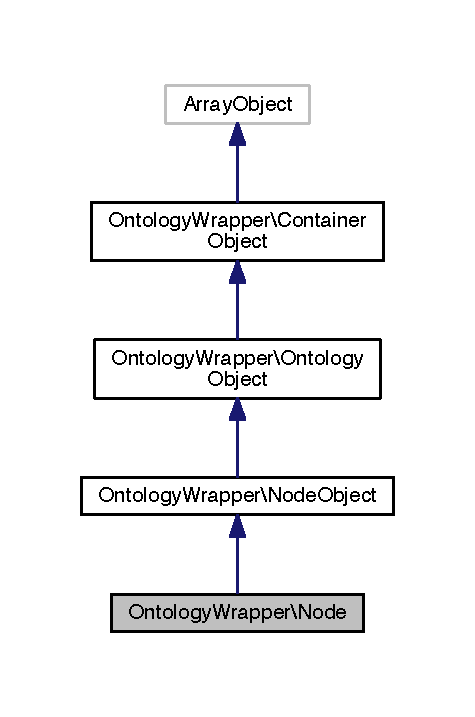
\includegraphics[width=228pt]{class_ontology_wrapper_1_1_node__inherit__graph}
\end{center}
\end{figure}


Collaboration diagram for Ontology\-Wrapper\textbackslash{}Node\-:
\nopagebreak
\begin{figure}[H]
\begin{center}
\leavevmode
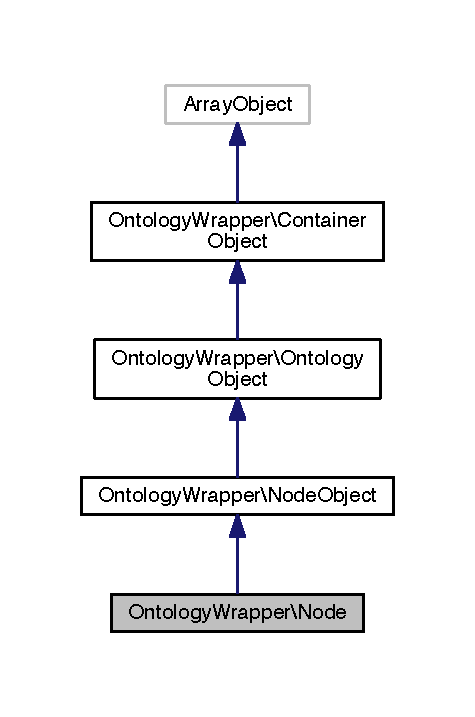
\includegraphics[width=228pt]{class_ontology_wrapper_1_1_node__coll__graph}
\end{center}
\end{figure}
\subsection*{Public Member Functions}
\begin{DoxyCompactItemize}
\item 
\hyperlink{class_ontology_wrapper_1_1_node_aa17f2c63c36277160e883deeb0b96134}{\-\_\-\-\_\-construct} (\$the\-Container=N\-U\-L\-L, \$the\-Identifier=N\-U\-L\-L)
\item 
\hyperlink{class_ontology_wrapper_1_1_node_ab1a39673329171326b6595d0c4cb782a}{load\-Tag} ()
\item 
\hyperlink{class_ontology_wrapper_1_1_node_a672ee5306bf9cb8c8c200f51a72e23e3}{load\-Term} ()
\item 
\hyperlink{class_ontology_wrapper_1_1_node_a01c318740fadbbb79d21513495e2b16a}{collect\-References} (\&\$the\-Container, \$do\-Object=T\-R\-U\-E)
\end{DoxyCompactItemize}
\subsection*{Static Public Member Functions}
\begin{DoxyCompactItemize}
\item 
static \hyperlink{class_ontology_wrapper_1_1_node_acd916b0222274569525e2a150a71b7dc}{Resolve\-Object} (\hyperlink{class_ontology_wrapper_1_1_connection_object}{Connection\-Object} \$the\-Connection, \$the\-Identifier, \$do\-Assert=T\-R\-U\-E)
\end{DoxyCompactItemize}
\subsection*{Public Attributes}
\begin{DoxyCompactItemize}
\item 
\hypertarget{class_ontology_wrapper_1_1_node_a17c5f694f51baf3410f6416753117521}{const {\bfseries k\-S\-E\-Q\-\_\-\-N\-A\-M\-E} = '\-\_\-nodes'}\label{class_ontology_wrapper_1_1_node_a17c5f694f51baf3410f6416753117521}

\end{DoxyCompactItemize}
\subsection*{Protected Member Functions}
\begin{DoxyCompactItemize}
\item 
\hyperlink{class_ontology_wrapper_1_1_node_a631f706a3a7f62fc5f1f75f42e5889e8}{pre\-Commit} (\$the\-Operation=0x00)
\item 
\hyperlink{class_ontology_wrapper_1_1_node_af777a6809d020b9ef64582373776a778}{post\-Commit} (\$the\-Operation=0x00)
\item 
\hyperlink{class_ontology_wrapper_1_1_node_af513e1e79f8c7dd360a3adb4265b315e}{is\-Ready} ()
\item 
\hyperlink{class_ontology_wrapper_1_1_node_ab8bf8f281ec784217a001a55b265ddfc}{post\-Offset\-Set} (\&\$the\-Offset, \&\$the\-Value)
\item 
\hyperlink{class_ontology_wrapper_1_1_node_ae5c0530b5499cdb995278fd63184a38a}{post\-Offset\-Unset} (\&\$the\-Offset)
\item 
\hyperlink{class_ontology_wrapper_1_1_node_aea89165149368db575c3da6fd4279785}{locked\-Offsets} ()
\end{DoxyCompactItemize}
\subsection*{Additional Inherited Members}


\subsection{Detailed Description}
\hyperlink{class_ontology_wrapper_1_1_node}{Node}

This class implements a persistent \hyperlink{class_ontology_wrapper_1_1_node_object}{Node\-Object} instance, the class concentrates on implementing all the necessary elements to ensure persistence to instances of this class and referential integrity.

The object is considered initialised, \hyperlink{namespace_ontology_wrapper_a7c06300cb0043d3bab108f92cb9be3db}{is\-Inited()}, if it has at least the term reference, \hyperlink{}{k\-T\-A\-G\-\_\-\-T\-E\-R\-M}, or the tag reference, \hyperlink{}{k\-T\-A\-G\-\_\-\-T\-A\-G}. \begin{DoxyVerb} @author            Milko A. Škofič <m.skofic@cgiar.org>
 @version   1.00 07/02/2014\end{DoxyVerb}
 

\subsection{Constructor \& Destructor Documentation}
\hypertarget{class_ontology_wrapper_1_1_node_aa17f2c63c36277160e883deeb0b96134}{\index{Ontology\-Wrapper\-::\-Node@{Ontology\-Wrapper\-::\-Node}!\-\_\-\-\_\-construct@{\-\_\-\-\_\-construct}}
\index{\-\_\-\-\_\-construct@{\-\_\-\-\_\-construct}!OntologyWrapper::Node@{Ontology\-Wrapper\-::\-Node}}
\subsubsection[{\-\_\-\-\_\-construct}]{\setlength{\rightskip}{0pt plus 5cm}Ontology\-Wrapper\textbackslash{}\-Node\-::\-\_\-\-\_\-construct (
\begin{DoxyParamCaption}
\item[{}]{\$the\-Container = {\ttfamily NULL}, }
\item[{}]{\$the\-Identifier = {\ttfamily NULL}}
\end{DoxyParamCaption}
)}}\label{class_ontology_wrapper_1_1_node_aa17f2c63c36277160e883deeb0b96134}
Instantiate class.

This constructor is standard for all persistent classes, we do nothing special here.


\begin{DoxyParams}[1]{Parameters}
\hyperlink{class_ontology_wrapper_1_1_connection_object}{Connection\-Object} & {\em \$the\-Container} & Persistent store. \\
\hline
mixed & {\em \$the\-Identifier} & Object identifier.\\
\hline
\end{DoxyParams}
public

\hyperlink{namespace_ontology_wrapper_ae6754181b2df357062755fcfe794a8b4}{instantiate\-Object()}

\begin{DoxySeeAlso}{See Also}
k\-T\-A\-G\-\_\-\-T\-A\-G k\-T\-A\-G\-\_\-\-T\-E\-R\-M 
\end{DoxySeeAlso}


\subsection{Member Function Documentation}
\hypertarget{class_ontology_wrapper_1_1_node_a01c318740fadbbb79d21513495e2b16a}{\index{Ontology\-Wrapper\-::\-Node@{Ontology\-Wrapper\-::\-Node}!collect\-References@{collect\-References}}
\index{collect\-References@{collect\-References}!OntologyWrapper::Node@{Ontology\-Wrapper\-::\-Node}}
\subsubsection[{collect\-References}]{\setlength{\rightskip}{0pt plus 5cm}Ontology\-Wrapper\textbackslash{}\-Node\-::collect\-References (
\begin{DoxyParamCaption}
\item[{\&}]{\$the\-Container, }
\item[{}]{\$do\-Object = {\ttfamily TRUE}}
\end{DoxyParamCaption}
)}}\label{class_ontology_wrapper_1_1_node_a01c318740fadbbb79d21513495e2b16a}
Collect references

In this class we collect the tag or term.


\begin{DoxyParams}[1]{Parameters}
reference & {\em \$the\-Container} & Receives objects. \\
\hline
boolean & {\em \$do\-Object} & {\ttfamily T\-R\-U\-E} load objects.\\
\hline
\end{DoxyParams}
public \hypertarget{class_ontology_wrapper_1_1_node_af513e1e79f8c7dd360a3adb4265b315e}{\index{Ontology\-Wrapper\-::\-Node@{Ontology\-Wrapper\-::\-Node}!is\-Ready@{is\-Ready}}
\index{is\-Ready@{is\-Ready}!OntologyWrapper::Node@{Ontology\-Wrapper\-::\-Node}}
\subsubsection[{is\-Ready}]{\setlength{\rightskip}{0pt plus 5cm}Ontology\-Wrapper\textbackslash{}\-Node\-::is\-Ready (
\begin{DoxyParamCaption}
{}
\end{DoxyParamCaption}
)\hspace{0.3cm}{\ttfamily [protected]}}}\label{class_ontology_wrapper_1_1_node_af513e1e79f8c7dd360a3adb4265b315e}
Check if object is ready

In this class we ensure the object has the native identifier, \hyperlink{}{k\-T\-A\-G\-\_\-\-N\-I\-D}, the global identifier,  k\-T\-A\-G\-\_\-\-P\-I\-D\}, the data type, \hyperlink{}{k\-T\-A\-G\-\_\-\-D\-A\-T\-A\-\_\-\-T\-Y\-P\-E}, and the label, \hyperlink{}{k\-T\-A\-G\-\_\-\-L\-A\-B\-E\-L}.

protected \begin{DoxyReturn}{Returns}
Boolean {\ttfamily T\-R\-U\-E} means ready. 
\end{DoxyReturn}
\hypertarget{class_ontology_wrapper_1_1_node_ab1a39673329171326b6595d0c4cb782a}{\index{Ontology\-Wrapper\-::\-Node@{Ontology\-Wrapper\-::\-Node}!load\-Tag@{load\-Tag}}
\index{load\-Tag@{load\-Tag}!OntologyWrapper::Node@{Ontology\-Wrapper\-::\-Node}}
\subsubsection[{load\-Tag}]{\setlength{\rightskip}{0pt plus 5cm}Ontology\-Wrapper\textbackslash{}\-Node\-::load\-Tag (
\begin{DoxyParamCaption}
{}
\end{DoxyParamCaption}
)}}\label{class_ontology_wrapper_1_1_node_ab1a39673329171326b6595d0c4cb782a}
Load tag object

This method can be used to resolve the tag into an object.

The method will return the tag object if the operation succeeded and {\ttfamily N\-U\-L\-L} if the object is not committed, if the object does not hold a collection reference, or if the object has no tag.

If the tag cannot be resolved, the method will raise an exception.

protected \begin{DoxyReturn}{Returns}
\hyperlink{class_ontology_wrapper_1_1_tag}{Tag} Resolved reference or {\ttfamily N\-U\-L\-L}. 
\end{DoxyReturn}
\hypertarget{class_ontology_wrapper_1_1_node_a672ee5306bf9cb8c8c200f51a72e23e3}{\index{Ontology\-Wrapper\-::\-Node@{Ontology\-Wrapper\-::\-Node}!load\-Term@{load\-Term}}
\index{load\-Term@{load\-Term}!OntologyWrapper::Node@{Ontology\-Wrapper\-::\-Node}}
\subsubsection[{load\-Term}]{\setlength{\rightskip}{0pt plus 5cm}Ontology\-Wrapper\textbackslash{}\-Node\-::load\-Term (
\begin{DoxyParamCaption}
{}
\end{DoxyParamCaption}
)}}\label{class_ontology_wrapper_1_1_node_a672ee5306bf9cb8c8c200f51a72e23e3}
Load term object

This method can be used to resolve the term into an object.

The method will return the term object if the operation succeeded and {\ttfamily N\-U\-L\-L} if the object is not committed, if the object does not hold a collection reference, or if the object has no term.

If the term cannot be resolved, the method will raise an exception.

protected \begin{DoxyReturn}{Returns}
\hyperlink{class_ontology_wrapper_1_1_term}{Term} Resolved reference or {\ttfamily N\-U\-L\-L}. 
\end{DoxyReturn}
\hypertarget{class_ontology_wrapper_1_1_node_aea89165149368db575c3da6fd4279785}{\index{Ontology\-Wrapper\-::\-Node@{Ontology\-Wrapper\-::\-Node}!locked\-Offsets@{locked\-Offsets}}
\index{locked\-Offsets@{locked\-Offsets}!OntologyWrapper::Node@{Ontology\-Wrapper\-::\-Node}}
\subsubsection[{locked\-Offsets}]{\setlength{\rightskip}{0pt plus 5cm}Ontology\-Wrapper\textbackslash{}\-Node\-::locked\-Offsets (
\begin{DoxyParamCaption}
{}
\end{DoxyParamCaption}
)\hspace{0.3cm}{\ttfamily [protected]}}}\label{class_ontology_wrapper_1_1_node_aea89165149368db575c3da6fd4279785}
Return list of locked offsets

In this class we return the static \hyperlink{}{\$s\-Internal\-Tags} list, the \hyperlink{}{k\-T\-A\-G\-\_\-\-P\-I\-D}, \hyperlink{}{k\-T\-A\-G\-\_\-\-T\-A\-G} and the \hyperlink{}{k\-T\-A\-G\-\_\-\-T\-E\-R\-M} offsets.

protected \begin{DoxyReturn}{Returns}
array List of locked offsets.
\end{DoxyReturn}
\begin{DoxySeeAlso}{See Also}
k\-T\-A\-G\-\_\-\-T\-A\-G k\-T\-A\-G\-\_\-\-T\-E\-R\-M 
\end{DoxySeeAlso}
\hypertarget{class_ontology_wrapper_1_1_node_af777a6809d020b9ef64582373776a778}{\index{Ontology\-Wrapper\-::\-Node@{Ontology\-Wrapper\-::\-Node}!post\-Commit@{post\-Commit}}
\index{post\-Commit@{post\-Commit}!OntologyWrapper::Node@{Ontology\-Wrapper\-::\-Node}}
\subsubsection[{post\-Commit}]{\setlength{\rightskip}{0pt plus 5cm}Ontology\-Wrapper\textbackslash{}\-Node\-::post\-Commit (
\begin{DoxyParamCaption}
\item[{}]{\$the\-Operation = {\ttfamily 0x00}}
\end{DoxyParamCaption}
)\hspace{0.3cm}{\ttfamily [protected]}}}\label{class_ontology_wrapper_1_1_node_af777a6809d020b9ef64582373776a778}
Cleanup object after commit

In this class we do nothing... yet.


\begin{DoxyParams}[1]{Parameters}
bitfield & {\em \$the\-Operation} & Operation code.\\
\hline
\end{DoxyParams}
protected \hypertarget{class_ontology_wrapper_1_1_node_ab8bf8f281ec784217a001a55b265ddfc}{\index{Ontology\-Wrapper\-::\-Node@{Ontology\-Wrapper\-::\-Node}!post\-Offset\-Set@{post\-Offset\-Set}}
\index{post\-Offset\-Set@{post\-Offset\-Set}!OntologyWrapper::Node@{Ontology\-Wrapper\-::\-Node}}
\subsubsection[{post\-Offset\-Set}]{\setlength{\rightskip}{0pt plus 5cm}Ontology\-Wrapper\textbackslash{}\-Node\-::post\-Offset\-Set (
\begin{DoxyParamCaption}
\item[{\&}]{\$the\-Offset, }
\item[{\&}]{\$the\-Value}
\end{DoxyParamCaption}
)\hspace{0.3cm}{\ttfamily [protected]}}}\label{class_ontology_wrapper_1_1_node_ab8bf8f281ec784217a001a55b265ddfc}
Handle offset and value after setting it

In this class we set the \hyperlink{namespace_ontology_wrapper_a7c06300cb0043d3bab108f92cb9be3db}{is\-Inited()} status.


\begin{DoxyParams}[1]{Parameters}
reference & {\em \$the\-Offset} & Offset reference. \\
\hline
reference & {\em \$the\-Value} & Offset value reference.\\
\hline
\end{DoxyParams}
protected

\begin{DoxySeeAlso}{See Also}
k\-T\-A\-G\-\_\-\-T\-A\-G k\-T\-A\-G\-\_\-\-T\-E\-R\-M 
\end{DoxySeeAlso}
\hypertarget{class_ontology_wrapper_1_1_node_ae5c0530b5499cdb995278fd63184a38a}{\index{Ontology\-Wrapper\-::\-Node@{Ontology\-Wrapper\-::\-Node}!post\-Offset\-Unset@{post\-Offset\-Unset}}
\index{post\-Offset\-Unset@{post\-Offset\-Unset}!OntologyWrapper::Node@{Ontology\-Wrapper\-::\-Node}}
\subsubsection[{post\-Offset\-Unset}]{\setlength{\rightskip}{0pt plus 5cm}Ontology\-Wrapper\textbackslash{}\-Node\-::post\-Offset\-Unset (
\begin{DoxyParamCaption}
\item[{\&}]{\$the\-Offset}
\end{DoxyParamCaption}
)\hspace{0.3cm}{\ttfamily [protected]}}}\label{class_ontology_wrapper_1_1_node_ae5c0530b5499cdb995278fd63184a38a}
Handle offset after deleting it

In this class we set the \hyperlink{namespace_ontology_wrapper_a7c06300cb0043d3bab108f92cb9be3db}{is\-Inited()} status.


\begin{DoxyParams}[1]{Parameters}
reference & {\em \$the\-Offset} & Offset reference.\\
\hline
\end{DoxyParams}
protected

\begin{DoxySeeAlso}{See Also}
k\-T\-A\-G\-\_\-\-T\-A\-G k\-T\-A\-G\-\_\-\-T\-E\-R\-M 
\end{DoxySeeAlso}
\hypertarget{class_ontology_wrapper_1_1_node_a631f706a3a7f62fc5f1f75f42e5889e8}{\index{Ontology\-Wrapper\-::\-Node@{Ontology\-Wrapper\-::\-Node}!pre\-Commit@{pre\-Commit}}
\index{pre\-Commit@{pre\-Commit}!OntologyWrapper::Node@{Ontology\-Wrapper\-::\-Node}}
\subsubsection[{pre\-Commit}]{\setlength{\rightskip}{0pt plus 5cm}Ontology\-Wrapper\textbackslash{}\-Node\-::pre\-Commit (
\begin{DoxyParamCaption}
\item[{}]{\$the\-Operation = {\ttfamily 0x00}}
\end{DoxyParamCaption}
)\hspace{0.3cm}{\ttfamily [protected]}}}\label{class_ontology_wrapper_1_1_node_a631f706a3a7f62fc5f1f75f42e5889e8}
Prepare object for commit

In this class we first check if the object is \hyperlink{namespace_ontology_wrapper_a7c06300cb0043d3bab108f92cb9be3db}{is\-Inited()}, if that is not the case, we raise an exception, since the object cannot be committed if not initialised.

We then set the native identifier with a sequence number, if not yet set.

When deleting we check whether the object has its native identifier.


\begin{DoxyParams}[1]{Parameters}
bitfield & {\em \$the\-Operation} & Operation code.\\
\hline
\end{DoxyParams}
protected

Exception \hypertarget{class_ontology_wrapper_1_1_node_acd916b0222274569525e2a150a71b7dc}{\index{Ontology\-Wrapper\-::\-Node@{Ontology\-Wrapper\-::\-Node}!Resolve\-Object@{Resolve\-Object}}
\index{Resolve\-Object@{Resolve\-Object}!OntologyWrapper::Node@{Ontology\-Wrapper\-::\-Node}}
\subsubsection[{Resolve\-Object}]{\setlength{\rightskip}{0pt plus 5cm}static Ontology\-Wrapper\textbackslash{}\-Node\-::\-Resolve\-Object (
\begin{DoxyParamCaption}
\item[{{\bf Connection\-Object}}]{\$the\-Connection, }
\item[{}]{\$the\-Identifier, }
\item[{}]{\$do\-Assert = {\ttfamily TRUE}}
\end{DoxyParamCaption}
)\hspace{0.3cm}{\ttfamily [static]}}}\label{class_ontology_wrapper_1_1_node_acd916b0222274569525e2a150a71b7dc}
Resolve object

This method can be used to statically instantiate an object from the provided data store, it will attempt to select the object matching the provided native identifier and return an instance of the originally committed class.

The method accepts the following parameters\-:


\begin{DoxyItemize}
\item {\bfseries \$the\-Container}\-: The database or collection from which the object is to be retrieved. 
\item {\bfseries \$the\-Identifier}\-: The objet native identifier. 
\item {\bfseries \$do\-Assert}\-: If {\ttfamily T\-R\-U\-E}, if the object is not matched, the method will raise an exception; if {\ttfamily F\-A\-L\-S\-E}, the method will return {\ttfamily N\-U\-L\-L}. 
\end{DoxyItemize}

We implement this method to match objects in the nodes collection.


\begin{DoxyParams}[1]{Parameters}
\hyperlink{class_ontology_wrapper_1_1_connection_object}{Connection\-Object} & {\em \$the\-Connection} & Persistent store. \\
\hline
mixed & {\em \$the\-Identifier} & Object identifier. \\
\hline
boolean & {\em \$do\-Assert} & Assert object.\\
\hline
\end{DoxyParams}
public \begin{DoxyReturn}{Returns}
\hyperlink{class_ontology_wrapper_1_1_ontology_object}{Ontology\-Object} Object or {\ttfamily N\-U\-L\-L}. 
\end{DoxyReturn}


The documentation for this class was generated from the following file\-:\begin{DoxyCompactItemize}
\item 
/\-Library/\-Web\-Server/\-Library/\-Ontology\-Wrapper/\-Library/\-Ontology\-Wrapper/Node.\-php\end{DoxyCompactItemize}

\hypertarget{class_ontology_wrapper_1_1_ontology_object}{\section{Ontology\-Wrapper\textbackslash{}Ontology\-Object Class Reference}
\label{class_ontology_wrapper_1_1_ontology_object}\index{Ontology\-Wrapper\textbackslash{}\-Ontology\-Object@{Ontology\-Wrapper\textbackslash{}\-Ontology\-Object}}
}


Inheritance diagram for Ontology\-Wrapper\textbackslash{}Ontology\-Object\-:\nopagebreak
\begin{figure}[H]
\begin{center}
\leavevmode
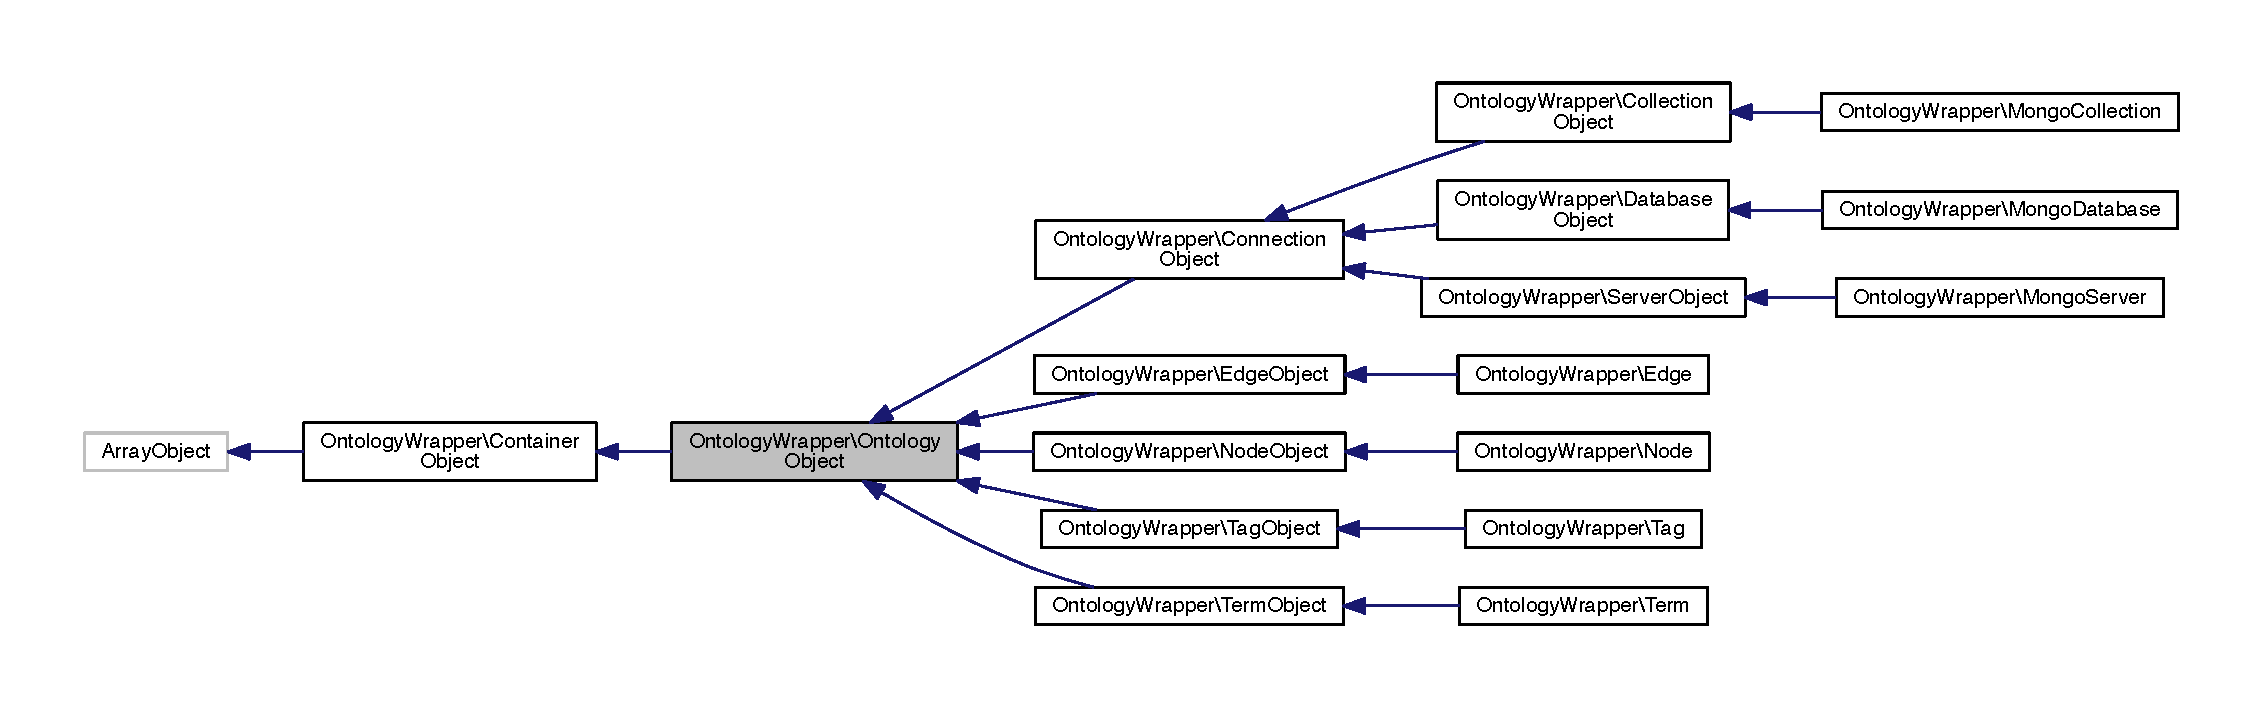
\includegraphics[width=350pt]{class_ontology_wrapper_1_1_ontology_object__inherit__graph}
\end{center}
\end{figure}


Collaboration diagram for Ontology\-Wrapper\textbackslash{}Ontology\-Object\-:\nopagebreak
\begin{figure}[H]
\begin{center}
\leavevmode
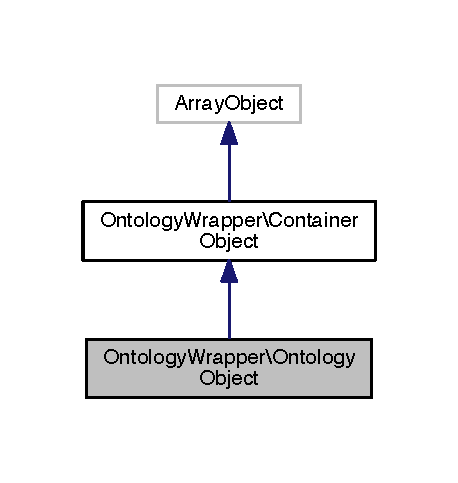
\includegraphics[width=220pt]{class_ontology_wrapper_1_1_ontology_object__coll__graph}
\end{center}
\end{figure}
\subsection*{Public Member Functions}
\begin{DoxyCompactItemize}
\item 
\hyperlink{class_ontology_wrapper_1_1_ontology_object_aa3f8d87842ea2c3a50b3e760adb2224f}{\-\_\-\-\_\-to\-String} ()
\item 
\hyperlink{class_ontology_wrapper_1_1_ontology_object_a28e1502b1cc43e05c07d854e79780e9c}{Reference} ()
\end{DoxyCompactItemize}
\subsection*{Static Public Member Functions}
\begin{DoxyCompactItemize}
\item 
static \hyperlink{class_ontology_wrapper_1_1_ontology_object_a12e1e673943d68230be1807bf6bd63cb}{Resolve\-Offset} (\$the\-Offset, \$do\-Assert=F\-A\-L\-S\-E)
\item 
static \hyperlink{class_ontology_wrapper_1_1_ontology_object_aa05e64fb4bbc9b30d15a8e2d1cfe9874}{Cast\-Offset\-Value} (\&\$the\-Value, \$the\-Offset, \$do\-Assert=F\-A\-L\-S\-E)
\end{DoxyCompactItemize}
\subsection*{Static Public Attributes}
\begin{DoxyCompactItemize}
\item 
\hypertarget{class_ontology_wrapper_1_1_ontology_object_a642b14dab22e6fd254de345a0b79f05b}{static {\bfseries \$s\-Internal\-Tags} = array( k\-T\-A\-G\-\_\-\-N\-I\-D, k\-T\-A\-G\-\_\-\-C\-L\-A\-S\-S )}\label{class_ontology_wrapper_1_1_ontology_object_a642b14dab22e6fd254de345a0b79f05b}

\end{DoxyCompactItemize}
\subsection*{Protected Member Functions}
\begin{DoxyCompactItemize}
\item 
\hyperlink{class_ontology_wrapper_1_1_ontology_object_aa8827d96f0f76ffdebde8346e331699c}{pre\-Offset\-Exists} (\&\$the\-Offset)
\item 
\hyperlink{class_ontology_wrapper_1_1_ontology_object_ab00c85a26561bf83f4721fa0edab5764}{pre\-Offset\-Get} (\&\$the\-Offset)
\item 
\hyperlink{class_ontology_wrapper_1_1_ontology_object_aa7e9b36fdc00584a143e6c920b6d2c87}{pre\-Offset\-Set} (\&\$the\-Offset, \&\$the\-Value)
\item 
\hyperlink{class_ontology_wrapper_1_1_ontology_object_a4ff5501f4fb4cf9fa88dbf5b3f845a1c}{pre\-Offset\-Unset} (\&\$the\-Offset)
\end{DoxyCompactItemize}


\subsection{Detailed Description}
Tags.

This file contains the default tag definitions. Types.

This file contains the default data type definitions. Tokens.

This file contains the default token definitions. Session.

This file contains the default session offset definitions. Ontology object

Objects derived from this {\itshape abstract} class hold two types of data\-: {\itshape run-\/time data}, which is stored in the object member properties and {\itshape persistent data}, which is stored in the inherited array part of the object.

The main purpose of this class is to ensure that all persistent data elements are {\itshape referenced}, {\itshape annotated} and {\itshape documented} in an ontology.

Persistent data is stored as {\itshape key/value} pair elements of the inherited array, the key part of the elements we call by convention {\itshape offset}, these offsets, in this class, represent a reference to an object of the ontology that holds all the necessary information to {\itshape identify}, {\itshape describe} and {\itshape validate} the value part of the array element pairs.

This class implements the bridge between object persistent data and the ontology, ensuring that all data holds a reference to the ontology, which, itself, is implemented by objects derived from this same class\-: this means that the whole system is self sufficient and self documenting.

Offsets can be uniquely identified in two ways\-: by native identifier, which is an integer value which may change across implementations, and a global identifier, which is a sring that will not change across implementations. This class provides a transparent interface that allows referring to offsets both by their {\itshape native} identifier or by their {\itshape global} identifier. Offsets, however, {\itshape will only hold the native identifier}, which means that all persistent data offsets must be integers. This is because global identifiers may become large strings, which poses a problem if these are used as field names for data stored in a persistent container.

Whenever the object is provided an offset, if this is a string, it will be fed to a static method, \hyperlink{class_ontology_wrapper_1_1_ontology_object_a12e1e673943d68230be1807bf6bd63cb}{Resolve\-Offset()}, which will check if the string represents the global identifier of an ontology \hyperlink{class_ontology_wrapper_1_1_tag}{Tag} object, in that case, the method will return the \hyperlink{class_ontology_wrapper_1_1_tag}{Tag}'s native integer identifier which will be used as the data offset. The class features a static data member, \hyperlink{}{\$s\-Internal\-Tags}, that holds the list of exceptions.

This means that to ensure referential integrity it is advisable to use integer constants as offsets when available, or string offsets if the integer constant is not known or available.

The resolution of these offsets is provided by a \hyperlink{class_ontology_wrapper_1_1_tag_cache}{Tag\-Cache} object which records all the {\itshape \hyperlink{class_ontology_wrapper_1_1_tag}{Tag}} objects of the ontology which are the entities that all offsets reference\-: persistent data offsets represent these \hyperlink{class_ontology_wrapper_1_1_tag}{Tag} native identifiers, while these \hyperlink{class_ontology_wrapper_1_1_tag}{Tag} object global identifiers are decoded by the \hyperlink{class_ontology_wrapper_1_1_tag_cache}{Tag\-Cache} object to retrieve the corresponding integer native identifier.

The class declares the \hyperlink{class_ontology_wrapper_1_1_ontology_object_aa3f8d87842ea2c3a50b3e760adb2224f}{\-\_\-\-\_\-to\-String()} method as virtual, it is essential that all derived classes implement this method which should return the current object's {\itshape global identifier string}. The global identifier of an object can be considered its signature or unique identifier, although a global identifier not need to be unique; all objects derived from this class, just as the \hyperlink{class_ontology_wrapper_1_1_tag}{Tag} object described above, must feature a global identifier, which may or may not coincide with their native identifier.

Finally, the class declares a method, \hyperlink{class_ontology_wrapper_1_1_ontology_object_a28e1502b1cc43e05c07d854e79780e9c}{Reference()}, which returns the current object's {\itshape reference}, this will generally be the value of the \hyperlink{}{k\-T\-A\-G\-\_\-\-N\-I\-D} offset. If the offset is not set, the method will raise an exception. This method will be put to use by derived classes\-: when providing an object to an offset expecting an object reference, by using this method one can be assured the provided object does have a reference. \begin{DoxyVerb} @author            Milko A. Škofič <m.skofic@cgiar.org>
 @version   1.00 10/01/2014\end{DoxyVerb}
 

\subsection{Member Function Documentation}
\hypertarget{class_ontology_wrapper_1_1_ontology_object_aa3f8d87842ea2c3a50b3e760adb2224f}{\index{Ontology\-Wrapper\-::\-Ontology\-Object@{Ontology\-Wrapper\-::\-Ontology\-Object}!\-\_\-\-\_\-to\-String@{\-\_\-\-\_\-to\-String}}
\index{\-\_\-\-\_\-to\-String@{\-\_\-\-\_\-to\-String}!OntologyWrapper::OntologyObject@{Ontology\-Wrapper\-::\-Ontology\-Object}}
\subsubsection[{\-\_\-\-\_\-to\-String}]{\setlength{\rightskip}{0pt plus 5cm}Ontology\-Wrapper\textbackslash{}\-Ontology\-Object\-::\-\_\-\-\_\-to\-String (
\begin{DoxyParamCaption}
{}
\end{DoxyParamCaption}
)\hspace{0.3cm}{\ttfamily [abstract]}}}\label{class_ontology_wrapper_1_1_ontology_object_aa3f8d87842ea2c3a50b3e760adb2224f}
\subparagraph*{Return global identifier}

This method should return the current object's global identifier.

All derived concrete classes must implement this method.

public \begin{DoxyReturn}{Returns}
string The global identifier. 
\end{DoxyReturn}
\hypertarget{class_ontology_wrapper_1_1_ontology_object_aa05e64fb4bbc9b30d15a8e2d1cfe9874}{\index{Ontology\-Wrapper\-::\-Ontology\-Object@{Ontology\-Wrapper\-::\-Ontology\-Object}!Cast\-Offset\-Value@{Cast\-Offset\-Value}}
\index{Cast\-Offset\-Value@{Cast\-Offset\-Value}!OntologyWrapper::OntologyObject@{Ontology\-Wrapper\-::\-Ontology\-Object}}
\subsubsection[{Cast\-Offset\-Value}]{\setlength{\rightskip}{0pt plus 5cm}static Ontology\-Wrapper\textbackslash{}\-Ontology\-Object\-::\-Cast\-Offset\-Value (
\begin{DoxyParamCaption}
\item[{\&}]{\$the\-Value, }
\item[{}]{\$the\-Offset, }
\item[{}]{\$do\-Assert = {\ttfamily FALSE}}
\end{DoxyParamCaption}
)\hspace{0.3cm}{\ttfamily [static]}}}\label{class_ontology_wrapper_1_1_ontology_object_aa05e64fb4bbc9b30d15a8e2d1cfe9874}
Cast offset

This method can be used to cast a value to the data type of its referred \hyperlink{class_ontology_wrapper_1_1_tag}{Tag}.

The method will first resolve the offset into a \hyperlink{class_ontology_wrapper_1_1_tag}{Tag} and then it will use the \hyperlink{class_ontology_wrapper_1_1_tag}{Tag}'s data type to cast the value.

The value will be cast only if the \hyperlink{class_ontology_wrapper_1_1_tag}{Tag} has {\itshape one} data type, if the provided value is an array, the method will cast each element to the data type.

If the method is unable to resolve the offset and the assert flag parameter is set, the method will raise an exception.

This method will handle in-\/line the data types of a series of default tags, this is necessary when loading the default ontology for the first time\-: since there are no tags in the system yet, any attempt to resolve these tags would fail; if you plan on changinf the data type of default tags, you should edit this method accordingly.


\begin{DoxyParams}[1]{Parameters}
reference & {\em \$the\-Value} & Value to cast. \\
\hline
mixed & {\em \$the\-Offset} & Data offset. \\
\hline
boolean & {\em \$do\-Assert} & Assert offset tag reference.\\
\hline
\end{DoxyParams}

\begin{DoxyExceptions}{Exceptions}
{\em Exception} & \\
\hline
\end{DoxyExceptions}
\begin{DoxySeeAlso}{See Also}
\$s\-Internal\-Tags 

k\-S\-E\-S\-S\-I\-O\-N\-\_\-\-D\-D\-I\-C\-T 
\end{DoxySeeAlso}
\hypertarget{class_ontology_wrapper_1_1_ontology_object_aa8827d96f0f76ffdebde8346e331699c}{\index{Ontology\-Wrapper\-::\-Ontology\-Object@{Ontology\-Wrapper\-::\-Ontology\-Object}!pre\-Offset\-Exists@{pre\-Offset\-Exists}}
\index{pre\-Offset\-Exists@{pre\-Offset\-Exists}!OntologyWrapper::OntologyObject@{Ontology\-Wrapper\-::\-Ontology\-Object}}
\subsubsection[{pre\-Offset\-Exists}]{\setlength{\rightskip}{0pt plus 5cm}Ontology\-Wrapper\textbackslash{}\-Ontology\-Object\-::pre\-Offset\-Exists (
\begin{DoxyParamCaption}
\item[{\&}]{\$the\-Offset}
\end{DoxyParamCaption}
)\hspace{0.3cm}{\ttfamily [protected]}}}\label{class_ontology_wrapper_1_1_ontology_object_aa8827d96f0f76ffdebde8346e331699c}
Handle offset before checking it

In this class we resolve the offset.


\begin{DoxyParams}[1]{Parameters}
reference & {\em \$the\-Offset} & Offset reference.\\
\hline
\end{DoxyParams}
protected \begin{DoxyReturn}{Returns}
mixed {\ttfamily N\-U\-L\-L} check offset, other, return.
\end{DoxyReturn}
\hyperlink{class_ontology_wrapper_1_1_ontology_object_a12e1e673943d68230be1807bf6bd63cb}{Resolve\-Offset()} \hypertarget{class_ontology_wrapper_1_1_ontology_object_ab00c85a26561bf83f4721fa0edab5764}{\index{Ontology\-Wrapper\-::\-Ontology\-Object@{Ontology\-Wrapper\-::\-Ontology\-Object}!pre\-Offset\-Get@{pre\-Offset\-Get}}
\index{pre\-Offset\-Get@{pre\-Offset\-Get}!OntologyWrapper::OntologyObject@{Ontology\-Wrapper\-::\-Ontology\-Object}}
\subsubsection[{pre\-Offset\-Get}]{\setlength{\rightskip}{0pt plus 5cm}Ontology\-Wrapper\textbackslash{}\-Ontology\-Object\-::pre\-Offset\-Get (
\begin{DoxyParamCaption}
\item[{\&}]{\$the\-Offset}
\end{DoxyParamCaption}
)\hspace{0.3cm}{\ttfamily [protected]}}}\label{class_ontology_wrapper_1_1_ontology_object_ab00c85a26561bf83f4721fa0edab5764}
Handle offset before getting it

In this class we resolve the offset.


\begin{DoxyParams}[1]{Parameters}
reference & {\em \$the\-Offset} & Offset reference.\\
\hline
\end{DoxyParams}
protected \begin{DoxyReturn}{Returns}
mixed {\ttfamily N\-U\-L\-L} get offset value, other, return.
\end{DoxyReturn}
\hyperlink{class_ontology_wrapper_1_1_ontology_object_a12e1e673943d68230be1807bf6bd63cb}{Resolve\-Offset()} \hypertarget{class_ontology_wrapper_1_1_ontology_object_aa7e9b36fdc00584a143e6c920b6d2c87}{\index{Ontology\-Wrapper\-::\-Ontology\-Object@{Ontology\-Wrapper\-::\-Ontology\-Object}!pre\-Offset\-Set@{pre\-Offset\-Set}}
\index{pre\-Offset\-Set@{pre\-Offset\-Set}!OntologyWrapper::OntologyObject@{Ontology\-Wrapper\-::\-Ontology\-Object}}
\subsubsection[{pre\-Offset\-Set}]{\setlength{\rightskip}{0pt plus 5cm}Ontology\-Wrapper\textbackslash{}\-Ontology\-Object\-::pre\-Offset\-Set (
\begin{DoxyParamCaption}
\item[{\&}]{\$the\-Offset, }
\item[{\&}]{\$the\-Value}
\end{DoxyParamCaption}
)\hspace{0.3cm}{\ttfamily [protected]}}}\label{class_ontology_wrapper_1_1_ontology_object_aa7e9b36fdc00584a143e6c920b6d2c87}
Handle offset and value before setting it

In this class we resolve the offset.


\begin{DoxyParams}[1]{Parameters}
reference & {\em \$the\-Offset} & Offset reference. \\
\hline
reference & {\em \$the\-Value} & Offset value reference.\\
\hline
\end{DoxyParams}
protected \begin{DoxyReturn}{Returns}
mixed {\ttfamily N\-U\-L\-L} set offset value, other, return.
\end{DoxyReturn}
\hyperlink{class_ontology_wrapper_1_1_ontology_object_a12e1e673943d68230be1807bf6bd63cb}{Resolve\-Offset()} \hypertarget{class_ontology_wrapper_1_1_ontology_object_a4ff5501f4fb4cf9fa88dbf5b3f845a1c}{\index{Ontology\-Wrapper\-::\-Ontology\-Object@{Ontology\-Wrapper\-::\-Ontology\-Object}!pre\-Offset\-Unset@{pre\-Offset\-Unset}}
\index{pre\-Offset\-Unset@{pre\-Offset\-Unset}!OntologyWrapper::OntologyObject@{Ontology\-Wrapper\-::\-Ontology\-Object}}
\subsubsection[{pre\-Offset\-Unset}]{\setlength{\rightskip}{0pt plus 5cm}Ontology\-Wrapper\textbackslash{}\-Ontology\-Object\-::pre\-Offset\-Unset (
\begin{DoxyParamCaption}
\item[{\&}]{\$the\-Offset}
\end{DoxyParamCaption}
)\hspace{0.3cm}{\ttfamily [protected]}}}\label{class_ontology_wrapper_1_1_ontology_object_a4ff5501f4fb4cf9fa88dbf5b3f845a1c}
Handle offset and value before deleting it

In this class we resolve the offset.


\begin{DoxyParams}[1]{Parameters}
reference & {\em \$the\-Offset} & Offset reference.\\
\hline
\end{DoxyParams}
protected \begin{DoxyReturn}{Returns}
mixed {\ttfamily N\-U\-L\-L} delete offset value, other, return.
\end{DoxyReturn}
\hyperlink{class_ontology_wrapper_1_1_ontology_object_a12e1e673943d68230be1807bf6bd63cb}{Resolve\-Offset()} \hypertarget{class_ontology_wrapper_1_1_ontology_object_a28e1502b1cc43e05c07d854e79780e9c}{\index{Ontology\-Wrapper\-::\-Ontology\-Object@{Ontology\-Wrapper\-::\-Ontology\-Object}!Reference@{Reference}}
\index{Reference@{Reference}!OntologyWrapper::OntologyObject@{Ontology\-Wrapper\-::\-Ontology\-Object}}
\subsubsection[{Reference}]{\setlength{\rightskip}{0pt plus 5cm}Ontology\-Wrapper\textbackslash{}\-Ontology\-Object\-::\-Reference (
\begin{DoxyParamCaption}
{}
\end{DoxyParamCaption}
)}}\label{class_ontology_wrapper_1_1_ontology_object_a28e1502b1cc43e05c07d854e79780e9c}
Return object reference

This method will return the current object's reference. This value should uniquely identify the referenced object, making it easy to retrieve the object given this reference.

In this class, and generally in all classes, the reference of an object is its native identifier, \hyperlink{}{k\-T\-A\-G\-\_\-\-N\-I\-D}.

The method must raise an exception if the reference cannot be provided.

public \begin{DoxyReturn}{Returns}
mixed Object reference.
\end{DoxyReturn}

\begin{DoxyExceptions}{Exceptions}
{\em Exception} & \\
\hline
\end{DoxyExceptions}
\hypertarget{class_ontology_wrapper_1_1_ontology_object_a12e1e673943d68230be1807bf6bd63cb}{\index{Ontology\-Wrapper\-::\-Ontology\-Object@{Ontology\-Wrapper\-::\-Ontology\-Object}!Resolve\-Offset@{Resolve\-Offset}}
\index{Resolve\-Offset@{Resolve\-Offset}!OntologyWrapper::OntologyObject@{Ontology\-Wrapper\-::\-Ontology\-Object}}
\subsubsection[{Resolve\-Offset}]{\setlength{\rightskip}{0pt plus 5cm}static Ontology\-Wrapper\textbackslash{}\-Ontology\-Object\-::\-Resolve\-Offset (
\begin{DoxyParamCaption}
\item[{}]{\$the\-Offset, }
\item[{}]{\$do\-Assert = {\ttfamily FALSE}}
\end{DoxyParamCaption}
)\hspace{0.3cm}{\ttfamily [static]}}}\label{class_ontology_wrapper_1_1_ontology_object_a12e1e673943d68230be1807bf6bd63cb}
Resolve offset

This method will resolve the provided offset into a \hyperlink{class_ontology_wrapper_1_1_tag_object}{Tag\-Object} native identifier, this is done by using a \hyperlink{class_ontology_wrapper_1_1_tag_cache}{Tag\-Cache} object stored in the \hyperlink{}{k\-S\-E\-S\-S\-I\-O\-N\-\_\-\-D\-D\-I\-C\-T} entry of the current session.

If you provide an integer or a numeric string, the method will simply cast the value to an integer and return it.

All other types of offsets, except those listed in the ststic \hyperlink{}{\$s\-Internal\-Tags} data member, will be used to locate the tag native identifier using a \hyperlink{class_ontology_wrapper_1_1_tag_cache}{Tag\-Cache} object stored in the \hyperlink{}{k\-S\-E\-S\-S\-I\-O\-N\-\_\-\-D\-D\-I\-C\-T} offset of the current session; if the provided offset cannot be resolved, the method will raise an exception if the second parameter is {\ttfamily T\-R\-U\-E}, or {\ttfamily N\-U\-L\-L} if the second parameter is {\ttfamily F\-A\-L\-S\-E}.

The method will raise an exception if the tag cache is not set.


\begin{DoxyParams}[1]{Parameters}
mixed & {\em \$the\-Offset} & Data offset. \\
\hline
boolean & {\em \$do\-Assert} & Assert offset tag reference.\\
\hline
\end{DoxyParams}
\begin{DoxyReturn}{Returns}
mixed Resolved offset.
\end{DoxyReturn}

\begin{DoxyExceptions}{Exceptions}
{\em Exception} & \\
\hline
\end{DoxyExceptions}
\begin{DoxySeeAlso}{See Also}
\$s\-Internal\-Tags 

k\-S\-E\-S\-S\-I\-O\-N\-\_\-\-D\-D\-I\-C\-T 
\end{DoxySeeAlso}


The documentation for this class was generated from the following file\-:\begin{DoxyCompactItemize}
\item 
/\-Library/\-Web\-Server/\-Library/\-Ontology\-Wrapper/\-Library/\-Ontology\-Wrapper/Ontology\-Object.\-php\end{DoxyCompactItemize}

\hypertarget{class_ontology_wrapper_1_1_persistent_object}{\section{Ontology\-Wrapper\textbackslash{}Persistent\-Object Class Reference}
\label{class_ontology_wrapper_1_1_persistent_object}\index{Ontology\-Wrapper\textbackslash{}\-Persistent\-Object@{Ontology\-Wrapper\textbackslash{}\-Persistent\-Object}}
}


Inheritance diagram for Ontology\-Wrapper\textbackslash{}Persistent\-Object\-:
\nopagebreak
\begin{figure}[H]
\begin{center}
\leavevmode
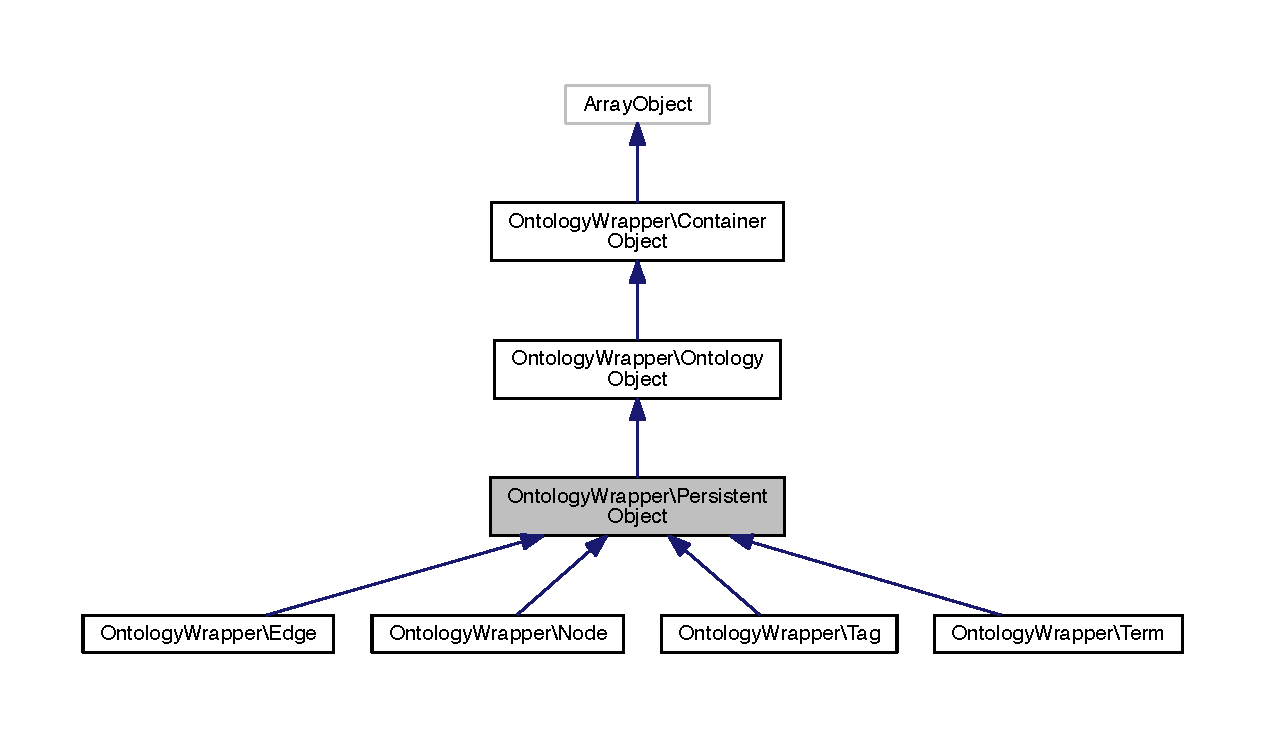
\includegraphics[width=350pt]{class_ontology_wrapper_1_1_persistent_object__inherit__graph}
\end{center}
\end{figure}


Collaboration diagram for Ontology\-Wrapper\textbackslash{}Persistent\-Object\-:
\nopagebreak
\begin{figure}[H]
\begin{center}
\leavevmode
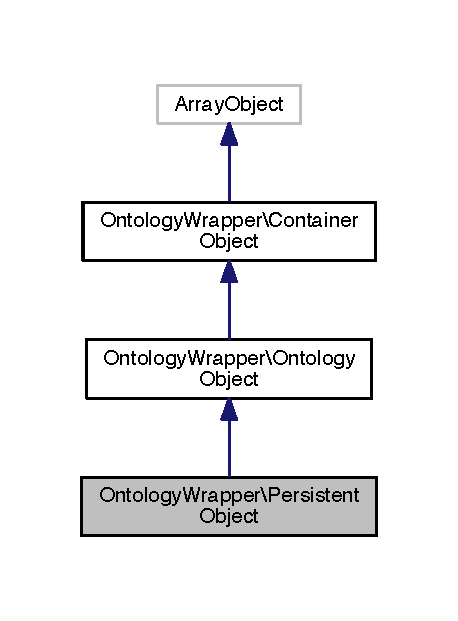
\includegraphics[width=220pt]{class_ontology_wrapper_1_1_persistent_object__coll__graph}
\end{center}
\end{figure}
\subsection*{Public Member Functions}
\begin{DoxyCompactItemize}
\item 
\hyperlink{class_ontology_wrapper_1_1_persistent_object_ac2375a2d3f51282a7d27bf62a3d3debc}{\-\_\-\-\_\-construct} (\$the\-Container=N\-U\-L\-L, \$the\-Identifier=N\-U\-L\-L)
\item 
\hyperlink{class_ontology_wrapper_1_1_persistent_object_ab9d702bee596c400b9403ea97583974e}{commit} (\hyperlink{class_ontology_wrapper_1_1_wrapper}{Wrapper} \$the\-Wrapper)
\end{DoxyCompactItemize}
\subsection*{Static Public Member Functions}
\begin{DoxyCompactItemize}
\item 
static \hyperlink{class_ontology_wrapper_1_1_persistent_object_a4103fc3005a33abe253a0a7250659da3}{Resolve\-Database} (\hyperlink{class_ontology_wrapper_1_1_wrapper}{Wrapper} \$the\-Wrapper, \$do\-Assert=T\-R\-U\-E, \$do\-Open=T\-R\-U\-E)
\item 
static \hyperlink{class_ontology_wrapper_1_1_persistent_object_a82580c299e95eda7cd28fa5bba1f8190}{Resolve\-Collection} (\hyperlink{class_ontology_wrapper_1_1_database_object}{Database\-Object} \$the\-Database, \$do\-Open=T\-R\-U\-E)
\end{DoxyCompactItemize}
\subsection*{Protected Member Functions}
\begin{DoxyCompactItemize}
\item 
\hyperlink{class_ontology_wrapper_1_1_persistent_object_ae621d7c6ec2b645d65ae86e6c183c7ef}{pre\-Commit} (\$the\-Operation=0x00)
\item 
\hyperlink{class_ontology_wrapper_1_1_persistent_object_a912920d6f5503319d971c6ec723d70fd}{pre\-Commit\-Validate} ()
\item 
\hyperlink{class_ontology_wrapper_1_1_persistent_object_ae6d939c963067e6553d31b02ee9c1e83}{pre\-Commit\-Identify} ()
\item 
\hyperlink{class_ontology_wrapper_1_1_persistent_object_a3eb6889a4ef15c0271561b45497b6a9d}{pre\-Commit\-Related} ()
\item 
\hyperlink{class_ontology_wrapper_1_1_persistent_object_a52d445c7c34fd2b28c48c4c47d02b1db}{post\-Commit} (\$the\-Operation=0x00)
\item 
\hyperlink{class_ontology_wrapper_1_1_persistent_object_abd1574b220543be97cb221fa2caded7a}{is\-Ready} ()
\item 
\hyperlink{class_ontology_wrapper_1_1_persistent_object_a20d852f3b8e527cab2e38f4ab54b6dad}{pre\-Offset\-Set} (\&\$the\-Offset, \&\$the\-Value)
\item 
\hyperlink{class_ontology_wrapper_1_1_persistent_object_af8ba5fa19459b094716006cad82bda7b}{post\-Offset\-Set} (\&\$the\-Offset, \&\$the\-Value)
\item 
\hyperlink{class_ontology_wrapper_1_1_persistent_object_a3a2f90f5bb97e7ebc1002f3ac77deab3}{pre\-Offset\-Unset} (\&\$the\-Offset)
\item 
\hyperlink{class_ontology_wrapper_1_1_persistent_object_abb77ffc2aa042528dc3129925f4b7764}{post\-Offset\-Unset} (\&\$the\-Offset)
\item 
\hyperlink{class_ontology_wrapper_1_1_persistent_object_ab539a5204bd58394d0a88353db957023}{locked\-Offsets} ()
\end{DoxyCompactItemize}
\subsection*{Additional Inherited Members}


\subsection{Detailed Description}
Persistent object

This {\itshape abstract} class is the ancestor of all classes representing objects that can persist in a container and that are constituted by ontology offsets.

The main purpose of this class is to add the status and persistence traits providing the prototypes needed to implement concrete persistent objects.

The class makes use of the \hyperlink{}{Status} and \hyperlink{}{Persistence} traits\-:


\begin{DoxyItemize}
\item {\ttfamily \hyperlink{}{Status}}\-: This class handles a bitfirld data member that keeps track of the object's status\-: 
\begin{DoxyItemize}
\item {\ttfamily \hyperlink{}{is\-Dirty()}}\-: This flag is set whenever any offset is modified, this status can be tested whenever the object should be stored in a persistent container\-: if set, it means the object has been modified, if not set, it means that the object is identical to the persistent copy. 
\item {\ttfamily \hyperlink{}{is\-Committed()}}\-: This flag is set whenever the object has been loaded or stored into a persistent container. This status can be useful to lock properties that cannot change once the object is stored. 
\end{DoxyItemize}
\item {\ttfamily \hyperlink{}{Persistence}}\-: This class handles the object persistence. 
\end{DoxyItemize}

Objects derived from this class {\itshape must} define a constant called {\itshape k\-S\-E\-Q\-\_\-\-N\-A\-M\-E} which provides a $<$em$<$string representing the {\itshape default collection name} for the current object\-: methods that commit or read objects of a specific class can then resolve the collection given a database. \begin{DoxyVerb} @author            Milko A. Škofič <m.skofic@cgiar.org>
 @version   1.00 14/02/2014\end{DoxyVerb}
 

\subsection{Constructor \& Destructor Documentation}
\hypertarget{class_ontology_wrapper_1_1_persistent_object_ac2375a2d3f51282a7d27bf62a3d3debc}{\index{Ontology\-Wrapper\-::\-Persistent\-Object@{Ontology\-Wrapper\-::\-Persistent\-Object}!\-\_\-\-\_\-construct@{\-\_\-\-\_\-construct}}
\index{\-\_\-\-\_\-construct@{\-\_\-\-\_\-construct}!OntologyWrapper::PersistentObject@{Ontology\-Wrapper\-::\-Persistent\-Object}}
\subsubsection[{\-\_\-\-\_\-construct}]{\setlength{\rightskip}{0pt plus 5cm}Ontology\-Wrapper\textbackslash{}\-Persistent\-Object\-::\-\_\-\-\_\-construct (
\begin{DoxyParamCaption}
\item[{}]{\$the\-Container = {\ttfamily NULL}, }
\item[{}]{\$the\-Identifier = {\ttfamily NULL}}
\end{DoxyParamCaption}
)}}\label{class_ontology_wrapper_1_1_persistent_object_ac2375a2d3f51282a7d27bf62a3d3debc}
Instantiate class.

Objects derived from this class share the same constructor prototype, they should not overload this method. The method accepts two parameters\-:


\begin{DoxyItemize}
\item {\bfseries \$the\-Container}\-: This may either be an array containing the object's persistent attributes, or a reference to a \hyperlink{class_ontology_wrapper_1_1_wrapper}{Wrapper} object. If this parameter is {\ttfamily N\-U\-L\-L}, the next parameter will be ignored. 
\item {\bfseries \$the\-Identifier}\-: This parameter represents the object identifier or the object persistent attributes\-: in the first case it will used to select the object from the provided container, in the second case, it is assumed that the provided array holds the persistent attributes of an object committed in the provided container. 
\end{DoxyItemize}

The workflow is as follows\-:


\begin{DoxyItemize}
\item {\itshape Empty object}\-: Both parameters are omitted. 
\item {\itshape Filled non committed object}\-: The first parameter is an array. 
\item {\itshape Load object from container}\-: The first parameter is a \hyperlink{class_ontology_wrapper_1_1_wrapper}{Wrapper} object and the second parameter is a scalar identifier. 
\item {\itshape Filled committed object}\-: The first parameter is \hyperlink{class_ontology_wrapper_1_1_wrapper}{Wrapper} object and the second parameter is an array holding the object's persistent data. 
\end{DoxyItemize}

Any other combination will raise an exception.

This constructor sets the committed flag, derived classes should first call the parent constructor, then they should set the inited flag.


\begin{DoxyParams}[1]{Parameters}
\hyperlink{class_ontology_wrapper_1_1_connection_object}{Connection\-Object} & {\em \$the\-Container} & Persistent store. \\
\hline
mixed & {\em \$the\-Identifier} & Object identifier.\\
\hline
\end{DoxyParams}
public


\begin{DoxyExceptions}{Exceptions}
{\em Exception} & \hyperlink{class_ontology_wrapper_1_1_persistent_object_a4103fc3005a33abe253a0a7250659da3}{Resolve\-Database()}  \hyperlink{class_ontology_wrapper_1_1_persistent_object_a82580c299e95eda7cd28fa5bba1f8190}{Resolve\-Collection()}  is\-Committed() \\
\hline
\end{DoxyExceptions}


\subsection{Member Function Documentation}
\hypertarget{class_ontology_wrapper_1_1_persistent_object_ab9d702bee596c400b9403ea97583974e}{\index{Ontology\-Wrapper\-::\-Persistent\-Object@{Ontology\-Wrapper\-::\-Persistent\-Object}!commit@{commit}}
\index{commit@{commit}!OntologyWrapper::PersistentObject@{Ontology\-Wrapper\-::\-Persistent\-Object}}
\subsubsection[{commit}]{\setlength{\rightskip}{0pt plus 5cm}Ontology\-Wrapper\textbackslash{}\-Persistent\-Object\-::commit (
\begin{DoxyParamCaption}
\item[{{\bf Wrapper}}]{\$the\-Wrapper}
\end{DoxyParamCaption}
)}}\label{class_ontology_wrapper_1_1_persistent_object_ab9d702bee596c400b9403ea97583974e}
Insert the object

This method should commit the current object into the provided persistent store.

In this method we perform the following steps\-:


\begin{DoxyItemize}
\item We resolve the eventually provided persistent store into a collection object, or we use the current object's collection; if this is not set, or if the collection canot be resolved, the method will raise an exception. 
\item We call the {\ttfamily \hyperlink{class_ontology_wrapper_1_1_persistent_object_ae621d7c6ec2b645d65ae86e6c183c7ef}{pre\-Commit()}} method that is responsible for preparing the object for being committed. 
\item If the object is not ready, \hyperlink{class_ontology_wrapper_1_1_persistent_object_abd1574b220543be97cb221fa2caded7a}{is\-Ready()}, we raise an exception. 
\item We pass the current object to the collection's commit method and recuperate the identifier. 
\item We call the {\ttfamily \hyperlink{class_ontology_wrapper_1_1_persistent_object_a52d445c7c34fd2b28c48c4c47d02b1db}{post\-Commit()}} method that is responsible of cleaning up the objecxt after the commit. 
\item We return the object's identifier. 
\end{DoxyItemize}

If any of the above steps fail the method must raise an exception.


\begin{DoxyParams}[1]{Parameters}
\hyperlink{class_ontology_wrapper_1_1_wrapper}{Wrapper} & {\em \$the\-Wrapper} & Persistent store.\\
\hline
\end{DoxyParams}
public \begin{DoxyReturn}{Returns}
mixed The object's native identifier.
\end{DoxyReturn}

\begin{DoxyExceptions}{Exceptions}
{\em Exception} & is\-Dirty()  is\-Committed()  \hyperlink{class_ontology_wrapper_1_1_ontology_object_a35bc67b94336aa801f20e495f3b0c3c2}{dictionary()}  \hyperlink{class_ontology_wrapper_1_1_persistent_object_a4103fc3005a33abe253a0a7250659da3}{Resolve\-Database()}  \hyperlink{class_ontology_wrapper_1_1_persistent_object_a82580c299e95eda7cd28fa5bba1f8190}{Resolve\-Collection()}  \hyperlink{class_ontology_wrapper_1_1_persistent_object_ae621d7c6ec2b645d65ae86e6c183c7ef}{pre\-Commit()}  \hyperlink{class_ontology_wrapper_1_1_persistent_object_abd1574b220543be97cb221fa2caded7a}{is\-Ready()}  \hyperlink{class_ontology_wrapper_1_1_persistent_object_a52d445c7c34fd2b28c48c4c47d02b1db}{post\-Commit()} \\
\hline
\end{DoxyExceptions}
\hypertarget{class_ontology_wrapper_1_1_persistent_object_abd1574b220543be97cb221fa2caded7a}{\index{Ontology\-Wrapper\-::\-Persistent\-Object@{Ontology\-Wrapper\-::\-Persistent\-Object}!is\-Ready@{is\-Ready}}
\index{is\-Ready@{is\-Ready}!OntologyWrapper::PersistentObject@{Ontology\-Wrapper\-::\-Persistent\-Object}}
\subsubsection[{is\-Ready}]{\setlength{\rightskip}{0pt plus 5cm}Ontology\-Wrapper\textbackslash{}\-Persistent\-Object\-::is\-Ready (
\begin{DoxyParamCaption}
{}
\end{DoxyParamCaption}
)\hspace{0.3cm}{\ttfamily [protected]}}}\label{class_ontology_wrapper_1_1_persistent_object_abd1574b220543be97cb221fa2caded7a}
Check if object is ready

This method should return {\ttfamily T\-R\-U\-E} if the object is ready to be committed.

In this class we ensure the object is initialised and that it holds the dictionary.

protected \begin{DoxyReturn}{Returns}
Boolean {\ttfamily T\-R\-U\-E} means ready. 
\end{DoxyReturn}
\hypertarget{class_ontology_wrapper_1_1_persistent_object_ab539a5204bd58394d0a88353db957023}{\index{Ontology\-Wrapper\-::\-Persistent\-Object@{Ontology\-Wrapper\-::\-Persistent\-Object}!locked\-Offsets@{locked\-Offsets}}
\index{locked\-Offsets@{locked\-Offsets}!OntologyWrapper::PersistentObject@{Ontology\-Wrapper\-::\-Persistent\-Object}}
\subsubsection[{locked\-Offsets}]{\setlength{\rightskip}{0pt plus 5cm}Ontology\-Wrapper\textbackslash{}\-Persistent\-Object\-::locked\-Offsets (
\begin{DoxyParamCaption}
{}
\end{DoxyParamCaption}
)\hspace{0.3cm}{\ttfamily [protected]}}}\label{class_ontology_wrapper_1_1_persistent_object_ab539a5204bd58394d0a88353db957023}
Return list of locked offsets

This method should return the list of locked offsets, that is, the offsets which cannot be modified once the object has been committed.

In this class we return the list of internal tags.

protected \begin{DoxyReturn}{Returns}
array List of locked offsets.
\end{DoxyReturn}
\hyperlink{class_ontology_wrapper_1_1_ontology_object_a1ec71ca3fd7be57916082804c1a30124}{Internal\-Offsets()} \hypertarget{class_ontology_wrapper_1_1_persistent_object_a52d445c7c34fd2b28c48c4c47d02b1db}{\index{Ontology\-Wrapper\-::\-Persistent\-Object@{Ontology\-Wrapper\-::\-Persistent\-Object}!post\-Commit@{post\-Commit}}
\index{post\-Commit@{post\-Commit}!OntologyWrapper::PersistentObject@{Ontology\-Wrapper\-::\-Persistent\-Object}}
\subsubsection[{post\-Commit}]{\setlength{\rightskip}{0pt plus 5cm}Ontology\-Wrapper\textbackslash{}\-Persistent\-Object\-::post\-Commit (
\begin{DoxyParamCaption}
\item[{}]{\$the\-Operation = {\ttfamily 0x00}}
\end{DoxyParamCaption}
)\hspace{0.3cm}{\ttfamily [protected]}}}\label{class_ontology_wrapper_1_1_persistent_object_a52d445c7c34fd2b28c48c4c47d02b1db}
Cleanup object after commit

This method should cleanup the object after it was committed, it should perform eventual identifiers and commit the eventual related objects.

The method accepts a single bitfield parameter that indicates the current operation\-:


\begin{DoxyItemize}
\item {\ttfamily 0x01}\-: Insert. 
\item {\ttfamily 0x11}\-: Update. 
\item {\ttfamily 0x10}\-: Delete. 
\end{DoxyItemize}

The first bit is set if the object is committed and the second bit is set if we are storing the object.

In this class we do nothing.


\begin{DoxyParams}[1]{Parameters}
bitfield & {\em \$the\-Operation} & Operation code.\\
\hline
\end{DoxyParams}
protected \hypertarget{class_ontology_wrapper_1_1_persistent_object_af8ba5fa19459b094716006cad82bda7b}{\index{Ontology\-Wrapper\-::\-Persistent\-Object@{Ontology\-Wrapper\-::\-Persistent\-Object}!post\-Offset\-Set@{post\-Offset\-Set}}
\index{post\-Offset\-Set@{post\-Offset\-Set}!OntologyWrapper::PersistentObject@{Ontology\-Wrapper\-::\-Persistent\-Object}}
\subsubsection[{post\-Offset\-Set}]{\setlength{\rightskip}{0pt plus 5cm}Ontology\-Wrapper\textbackslash{}\-Persistent\-Object\-::post\-Offset\-Set (
\begin{DoxyParamCaption}
\item[{\&}]{\$the\-Offset, }
\item[{\&}]{\$the\-Value}
\end{DoxyParamCaption}
)\hspace{0.3cm}{\ttfamily [protected]}}}\label{class_ontology_wrapper_1_1_persistent_object_af8ba5fa19459b094716006cad82bda7b}
Handle offset and value after setting it

We overload the parent method to set the \hyperlink{}{is\-Dirty()} status.

In this class we do nothing.


\begin{DoxyParams}[1]{Parameters}
reference & {\em \$the\-Offset} & Offset reference. \\
\hline
reference & {\em \$the\-Value} & Offset value reference.\\
\hline
\end{DoxyParams}
protected

is\-Dirty() \hypertarget{class_ontology_wrapper_1_1_persistent_object_abb77ffc2aa042528dc3129925f4b7764}{\index{Ontology\-Wrapper\-::\-Persistent\-Object@{Ontology\-Wrapper\-::\-Persistent\-Object}!post\-Offset\-Unset@{post\-Offset\-Unset}}
\index{post\-Offset\-Unset@{post\-Offset\-Unset}!OntologyWrapper::PersistentObject@{Ontology\-Wrapper\-::\-Persistent\-Object}}
\subsubsection[{post\-Offset\-Unset}]{\setlength{\rightskip}{0pt plus 5cm}Ontology\-Wrapper\textbackslash{}\-Persistent\-Object\-::post\-Offset\-Unset (
\begin{DoxyParamCaption}
\item[{\&}]{\$the\-Offset}
\end{DoxyParamCaption}
)\hspace{0.3cm}{\ttfamily [protected]}}}\label{class_ontology_wrapper_1_1_persistent_object_abb77ffc2aa042528dc3129925f4b7764}
Handle offset after deleting it

This method can be used to manage the object after calling the \hyperlink{}{Array\-Object\-::\-Offset\-Unset()} method.

In this class we do nothing.


\begin{DoxyParams}[1]{Parameters}
reference & {\em \$the\-Offset} & Offset reference.\\
\hline
\end{DoxyParams}
protected

is\-Dirty() \hypertarget{class_ontology_wrapper_1_1_persistent_object_ae621d7c6ec2b645d65ae86e6c183c7ef}{\index{Ontology\-Wrapper\-::\-Persistent\-Object@{Ontology\-Wrapper\-::\-Persistent\-Object}!pre\-Commit@{pre\-Commit}}
\index{pre\-Commit@{pre\-Commit}!OntologyWrapper::PersistentObject@{Ontology\-Wrapper\-::\-Persistent\-Object}}
\subsubsection[{pre\-Commit}]{\setlength{\rightskip}{0pt plus 5cm}Ontology\-Wrapper\textbackslash{}\-Persistent\-Object\-::pre\-Commit (
\begin{DoxyParamCaption}
\item[{}]{\$the\-Operation = {\ttfamily 0x00}}
\end{DoxyParamCaption}
)\hspace{0.3cm}{\ttfamily [protected]}}}\label{class_ontology_wrapper_1_1_persistent_object_ae621d7c6ec2b645d65ae86e6c183c7ef}
Prepare object for commit

This method should prepare the object for being committed, it should compute the eventual identifiers and commit the eventual related objects.

The method accepts a single bitfield parameter that indicates the current operation\-: the first bit is set if the object is committed and the second bit is set if we are storing the object.


\begin{DoxyItemize}
\item {\ttfamily 0x01}\-: {\itshape Insert} 
\begin{DoxyItemize}
\item Check if the object is \hyperlink{}{is\-Inited()}. 
\item {\ttfamily \hyperlink{class_ontology_wrapper_1_1_persistent_object_a912920d6f5503319d971c6ec723d70fd}{\-: Validate object. }{\ttfamily \hyperlink{class_ontology_wrapper_1_1_persistent_object_ae6d939c963067e6553d31b02ee9c1e83}{\-: Set object identifiers. }{\ttfamily \hyperlink{class_ontology_wrapper_1_1_persistent_object_abd1574b220543be97cb221fa2caded7a}{\-: Check if object is ready. }{\ttfamily \hyperlink{class_ontology_wrapper_1_1_persistent_object_a3eb6889a4ef15c0271561b45497b6a9d}{\-: Commit related objects. } }}}}
\item {\ttfamily {\ttfamily {\ttfamily {\ttfamily {\ttfamily 0x11}\-: {\itshape Update} 
\begin{DoxyItemize}
\item Nothing yet (this operation should not be implemented). 
\end{DoxyItemize}}}}}
\item {\ttfamily {\ttfamily {\ttfamily {\ttfamily {\ttfamily 0x10}\-: {\itshape Delete} 
\begin{DoxyItemize}
\item Check if the object has its native identifier, \hyperlink{}{k\-T\-A\-G\-\_\-\-N\-I\-D}. 
\end{DoxyItemize}}}}}
\end{DoxyItemize}

{\ttfamily {\ttfamily {\ttfamily {\ttfamily Derived classes should not overload this method, they should, instead, overload the called methods.}}}}

{\ttfamily {\ttfamily {\ttfamily {\ttfamily 
\begin{DoxyParams}[1]{Parameters}
bitfield & {\em \$the\-Operation} & Operation code.\\
\hline
\end{DoxyParams}
protected}}}}

{\ttfamily {\ttfamily {\ttfamily {\ttfamily 
\begin{DoxyExceptions}{Exceptions}
{\em Exception} & \\
\hline
\end{DoxyExceptions}
\begin{DoxySeeAlso}{See Also}
k\-T\-A\-G\-\_\-\-N\-I\-D
\end{DoxySeeAlso}
is\-Inited() }}}}
\end{DoxyItemize}\hypertarget{class_ontology_wrapper_1_1_persistent_object_ae6d939c963067e6553d31b02ee9c1e83}{\index{Ontology\-Wrapper\-::\-Persistent\-Object@{Ontology\-Wrapper\-::\-Persistent\-Object}!pre\-Commit\-Identify@{pre\-Commit\-Identify}}
\index{pre\-Commit\-Identify@{pre\-Commit\-Identify}!OntologyWrapper::PersistentObject@{Ontology\-Wrapper\-::\-Persistent\-Object}}
\subsubsection[{pre\-Commit\-Identify}]{\setlength{\rightskip}{0pt plus 5cm}Ontology\-Wrapper\textbackslash{}\-Persistent\-Object\-::pre\-Commit\-Identify (
\begin{DoxyParamCaption}
{}
\end{DoxyParamCaption}
)\hspace{0.3cm}{\ttfamily [abstract]}, {\ttfamily [protected]}}}\label{class_ontology_wrapper_1_1_persistent_object_ae6d939c963067e6553d31b02ee9c1e83}
Set object identifiers before commit

This method should set the object identifiers.

Derived classes must implement this method and should not overload the caller.

protected \hypertarget{class_ontology_wrapper_1_1_persistent_object_a3eb6889a4ef15c0271561b45497b6a9d}{\index{Ontology\-Wrapper\-::\-Persistent\-Object@{Ontology\-Wrapper\-::\-Persistent\-Object}!pre\-Commit\-Related@{pre\-Commit\-Related}}
\index{pre\-Commit\-Related@{pre\-Commit\-Related}!OntologyWrapper::PersistentObject@{Ontology\-Wrapper\-::\-Persistent\-Object}}
\subsubsection[{pre\-Commit\-Related}]{\setlength{\rightskip}{0pt plus 5cm}Ontology\-Wrapper\textbackslash{}\-Persistent\-Object\-::pre\-Commit\-Related (
\begin{DoxyParamCaption}
{}
\end{DoxyParamCaption}
)\hspace{0.3cm}{\ttfamily [abstract]}, {\ttfamily [protected]}}}\label{class_ontology_wrapper_1_1_persistent_object_a3eb6889a4ef15c0271561b45497b6a9d}
Commit related objects

This method should commit related objects before the current object is committed.

Derived classes must implement this method and should not overload the caller.

protected \hypertarget{class_ontology_wrapper_1_1_persistent_object_a912920d6f5503319d971c6ec723d70fd}{\index{Ontology\-Wrapper\-::\-Persistent\-Object@{Ontology\-Wrapper\-::\-Persistent\-Object}!pre\-Commit\-Validate@{pre\-Commit\-Validate}}
\index{pre\-Commit\-Validate@{pre\-Commit\-Validate}!OntologyWrapper::PersistentObject@{Ontology\-Wrapper\-::\-Persistent\-Object}}
\subsubsection[{pre\-Commit\-Validate}]{\setlength{\rightskip}{0pt plus 5cm}Ontology\-Wrapper\textbackslash{}\-Persistent\-Object\-::pre\-Commit\-Validate (
\begin{DoxyParamCaption}
{}
\end{DoxyParamCaption}
)\hspace{0.3cm}{\ttfamily [abstract]}, {\ttfamily [protected]}}}\label{class_ontology_wrapper_1_1_persistent_object_a912920d6f5503319d971c6ec723d70fd}
Validate object before commit

This method should validate the object before being committed.

Derived classes must implement this method and should not overload the caller.

protected \hypertarget{class_ontology_wrapper_1_1_persistent_object_a20d852f3b8e527cab2e38f4ab54b6dad}{\index{Ontology\-Wrapper\-::\-Persistent\-Object@{Ontology\-Wrapper\-::\-Persistent\-Object}!pre\-Offset\-Set@{pre\-Offset\-Set}}
\index{pre\-Offset\-Set@{pre\-Offset\-Set}!OntologyWrapper::PersistentObject@{Ontology\-Wrapper\-::\-Persistent\-Object}}
\subsubsection[{pre\-Offset\-Set}]{\setlength{\rightskip}{0pt plus 5cm}Ontology\-Wrapper\textbackslash{}\-Persistent\-Object\-::pre\-Offset\-Set (
\begin{DoxyParamCaption}
\item[{\&}]{\$the\-Offset, }
\item[{\&}]{\$the\-Value}
\end{DoxyParamCaption}
)\hspace{0.3cm}{\ttfamily [protected]}}}\label{class_ontology_wrapper_1_1_persistent_object_a20d852f3b8e527cab2e38f4ab54b6dad}
Handle offset and value before setting it

We overload this method to prevent modifying the global and native identifiers if the object is committed, \hyperlink{}{is\-Committed()}.


\begin{DoxyParams}[1]{Parameters}
reference & {\em \$the\-Offset} & Offset reference. \\
\hline
reference & {\em \$the\-Value} & Offset value reference.\\
\hline
\end{DoxyParams}
protected \begin{DoxyReturn}{Returns}
mixed {\ttfamily N\-U\-L\-L} set offset value, other, return.
\end{DoxyReturn}

\begin{DoxyExceptions}{Exceptions}
{\em Exception} & is\-Committed()  \hyperlink{class_ontology_wrapper_1_1_ontology_object_a1ec71ca3fd7be57916082804c1a30124}{Internal\-Offsets()} \\
\hline
\end{DoxyExceptions}
\hypertarget{class_ontology_wrapper_1_1_persistent_object_a3a2f90f5bb97e7ebc1002f3ac77deab3}{\index{Ontology\-Wrapper\-::\-Persistent\-Object@{Ontology\-Wrapper\-::\-Persistent\-Object}!pre\-Offset\-Unset@{pre\-Offset\-Unset}}
\index{pre\-Offset\-Unset@{pre\-Offset\-Unset}!OntologyWrapper::PersistentObject@{Ontology\-Wrapper\-::\-Persistent\-Object}}
\subsubsection[{pre\-Offset\-Unset}]{\setlength{\rightskip}{0pt plus 5cm}Ontology\-Wrapper\textbackslash{}\-Persistent\-Object\-::pre\-Offset\-Unset (
\begin{DoxyParamCaption}
\item[{\&}]{\$the\-Offset}
\end{DoxyParamCaption}
)\hspace{0.3cm}{\ttfamily [protected]}}}\label{class_ontology_wrapper_1_1_persistent_object_a3a2f90f5bb97e7ebc1002f3ac77deab3}
Handle offset and value before deleting it

We overload this method to prevent modifying the global and native identifiers if the object is committed, \hyperlink{}{is\-Committed()}.


\begin{DoxyParams}[1]{Parameters}
reference & {\em \$the\-Offset} & Offset reference.\\
\hline
\end{DoxyParams}
protected \begin{DoxyReturn}{Returns}
mixed {\ttfamily N\-U\-L\-L} delete offset value, other, return.
\end{DoxyReturn}

\begin{DoxyExceptions}{Exceptions}
{\em Exception} & is\-Committed()  \hyperlink{class_ontology_wrapper_1_1_persistent_object_ab539a5204bd58394d0a88353db957023}{locked\-Offsets()} \\
\hline
\end{DoxyExceptions}
\hypertarget{class_ontology_wrapper_1_1_persistent_object_a82580c299e95eda7cd28fa5bba1f8190}{\index{Ontology\-Wrapper\-::\-Persistent\-Object@{Ontology\-Wrapper\-::\-Persistent\-Object}!Resolve\-Collection@{Resolve\-Collection}}
\index{Resolve\-Collection@{Resolve\-Collection}!OntologyWrapper::PersistentObject@{Ontology\-Wrapper\-::\-Persistent\-Object}}
\subsubsection[{Resolve\-Collection}]{\setlength{\rightskip}{0pt plus 5cm}static Ontology\-Wrapper\textbackslash{}\-Persistent\-Object\-::\-Resolve\-Collection (
\begin{DoxyParamCaption}
\item[{{\bf Database\-Object}}]{\$the\-Database, }
\item[{}]{\$do\-Open = {\ttfamily TRUE}}
\end{DoxyParamCaption}
)\hspace{0.3cm}{\ttfamily [static]}}}\label{class_ontology_wrapper_1_1_persistent_object_a82580c299e95eda7cd28fa5bba1f8190}
Resolve the collection

This method should return a \hyperlink{class_ontology_wrapper_1_1_collection_object}{Collection\-Object} instance corresponding to the persistent store in which the current object was either read or will be inserted.

The method expects the object to feature a constant, \hyperlink{}{k\-S\-E\-Q\-\_\-\-N\-A\-M\-E}, which serves the double purpose of providing the default collection name and the eventual sequence number index\-: the method will use this constant and the provided database reference to return the default \hyperlink{class_ontology_wrapper_1_1_collection_object}{Collection\-Object} instance.


\begin{DoxyParams}[1]{Parameters}
\hyperlink{class_ontology_wrapper_1_1_database_object}{Database\-Object} & {\em \$the\-Database} & Database reference. \\
\hline
boolean & {\em \$do\-Open} & {\ttfamily T\-R\-U\-E} open connection.\\
\hline
\end{DoxyParams}
\begin{DoxyReturn}{Returns}
\hyperlink{class_ontology_wrapper_1_1_collection_object}{Collection\-Object} Collection or {\ttfamily N\-U\-L\-L}. 
\end{DoxyReturn}
\hypertarget{class_ontology_wrapper_1_1_persistent_object_a4103fc3005a33abe253a0a7250659da3}{\index{Ontology\-Wrapper\-::\-Persistent\-Object@{Ontology\-Wrapper\-::\-Persistent\-Object}!Resolve\-Database@{Resolve\-Database}}
\index{Resolve\-Database@{Resolve\-Database}!OntologyWrapper::PersistentObject@{Ontology\-Wrapper\-::\-Persistent\-Object}}
\subsubsection[{Resolve\-Database}]{\setlength{\rightskip}{0pt plus 5cm}static Ontology\-Wrapper\textbackslash{}\-Persistent\-Object\-::\-Resolve\-Database (
\begin{DoxyParamCaption}
\item[{{\bf Wrapper}}]{\$the\-Wrapper, }
\item[{}]{\$do\-Assert = {\ttfamily TRUE}, }
\item[{}]{\$do\-Open = {\ttfamily TRUE}}
\end{DoxyParamCaption}
)\hspace{0.3cm}{\ttfamily [static]}}}\label{class_ontology_wrapper_1_1_persistent_object_a4103fc3005a33abe253a0a7250659da3}
Resolve the database

This method should return a \hyperlink{class_ontology_wrapper_1_1_database_object}{Database\-Object} instance corresponding to the default database of the current class extracted from the provided \hyperlink{class_ontology_wrapper_1_1_wrapper}{Wrapper} instance.

Since we cannot declare this method abstract, we raise an exception.


\begin{DoxyParams}[1]{Parameters}
\hyperlink{class_ontology_wrapper_1_1_wrapper}{Wrapper} & {\em \$the\-Wrapper} & \hyperlink{class_ontology_wrapper_1_1_wrapper}{Wrapper}. \\
\hline
boolean & {\em \$do\-Assert} & Raise exception if unable. \\
\hline
boolean & {\em \$do\-Open} & {\ttfamily T\-R\-U\-E} open connection.\\
\hline
\end{DoxyParams}
\begin{DoxyReturn}{Returns}
\hyperlink{class_ontology_wrapper_1_1_database_object}{Database\-Object} Database or {\ttfamily N\-U\-L\-L}.
\end{DoxyReturn}

\begin{DoxyExceptions}{Exceptions}
{\em Exception} & \\
\hline
\end{DoxyExceptions}


The documentation for this class was generated from the following file\-:\begin{DoxyCompactItemize}
\item 
/\-Library/\-Web\-Server/\-Library/\-Ontology\-Wrapper/\-Library/\-Ontology\-Wrapper/Persistent\-Object.\-php\end{DoxyCompactItemize}

\hypertarget{class_ontology_wrapper_1_1_server_object}{\section{Ontology\-Wrapper\textbackslash{}Server\-Object Class Reference}
\label{class_ontology_wrapper_1_1_server_object}\index{Ontology\-Wrapper\textbackslash{}\-Server\-Object@{Ontology\-Wrapper\textbackslash{}\-Server\-Object}}
}


Inheritance diagram for Ontology\-Wrapper\textbackslash{}Server\-Object\-:\nopagebreak
\begin{figure}[H]
\begin{center}
\leavevmode
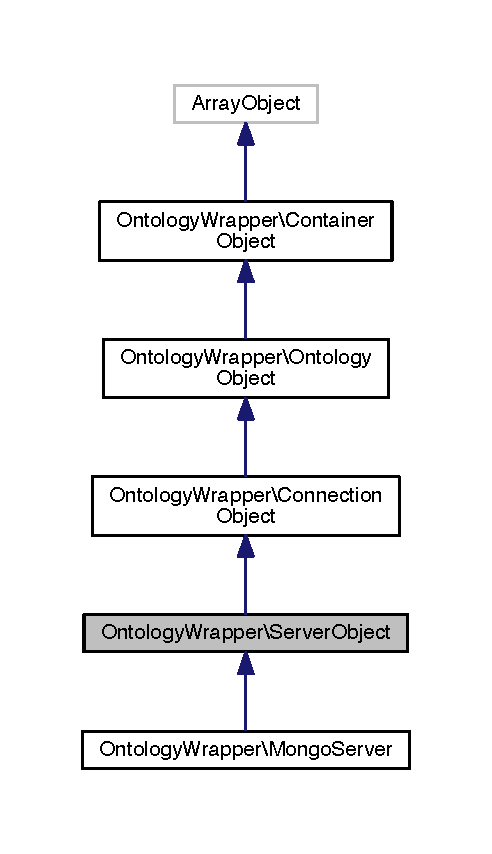
\includegraphics[width=236pt]{class_ontology_wrapper_1_1_server_object__inherit__graph}
\end{center}
\end{figure}


Collaboration diagram for Ontology\-Wrapper\textbackslash{}Server\-Object\-:\nopagebreak
\begin{figure}[H]
\begin{center}
\leavevmode
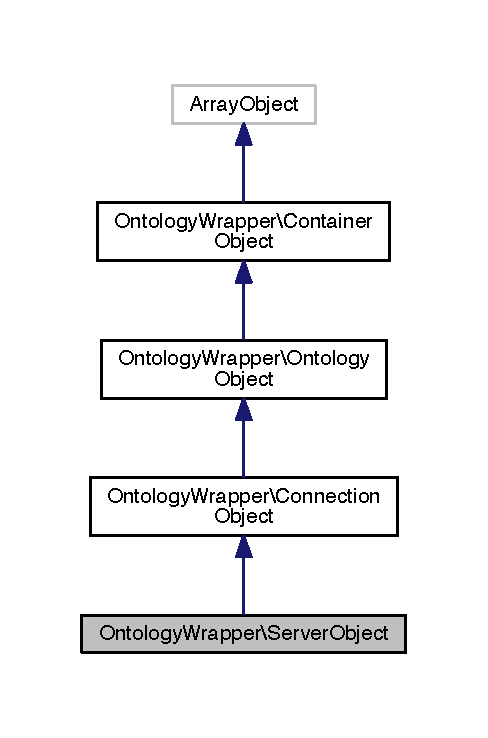
\includegraphics[width=234pt]{class_ontology_wrapper_1_1_server_object__coll__graph}
\end{center}
\end{figure}
\subsection*{Public Member Functions}
\begin{DoxyCompactItemize}
\item 
\hyperlink{class_ontology_wrapper_1_1_server_object_a3ce047db243e208640e8eaf89b986c7a}{Database} (\$the\-Name)
\item 
\hyperlink{class_ontology_wrapper_1_1_server_object_afdff50c16982e3266578d75d1fb19dea}{get\-Statistics} ()
\end{DoxyCompactItemize}
\subsection*{Static Public Attributes}
\begin{DoxyCompactItemize}
\item 
static {\bfseries \$s\-Offsets}
\end{DoxyCompactItemize}
\subsection*{Protected Member Functions}
\begin{DoxyCompactItemize}
\item 
\hyperlink{class_ontology_wrapper_1_1_server_object_a0ba24c5513d7b5dc168a0d058adb2aca}{new\-Database} (\$the\-Offsets)
\end{DoxyCompactItemize}
\subsection*{Additional Inherited Members}


\subsection{Detailed Description}
Server object

This {\itshape abstract} class is the ancestor of all classes representing server connection instances, this class extends the \hyperlink{class_ontology_wrapper_1_1_connection_object}{Connection\-Object} class to implement server specific functionality prototypes. \begin{DoxyVerb} @author            Milko A. Škofič <m.skofic@cgiar.org>
 @version   1.00 06/02/2014\end{DoxyVerb}
 

\subsection{Member Function Documentation}
\hypertarget{class_ontology_wrapper_1_1_server_object_a3ce047db243e208640e8eaf89b986c7a}{\index{Ontology\-Wrapper\-::\-Server\-Object@{Ontology\-Wrapper\-::\-Server\-Object}!Database@{Database}}
\index{Database@{Database}!OntologyWrapper::ServerObject@{Ontology\-Wrapper\-::\-Server\-Object}}
\subsubsection[{Database}]{\setlength{\rightskip}{0pt plus 5cm}Ontology\-Wrapper\textbackslash{}\-Server\-Object\-::\-Database (
\begin{DoxyParamCaption}
\item[{}]{\$the\-Name}
\end{DoxyParamCaption}
)}}\label{class_ontology_wrapper_1_1_server_object_a3ce047db243e208640e8eaf89b986c7a}
Return database connection

This method can be used to return a database connection from the current server.

The method expects a single parameter which represents the database name, the method should return an instance of a class derived from \hyperlink{class_ontology_wrapper_1_1_database_object}{Database\-Object}.


\begin{DoxyParams}[1]{Parameters}
string & {\em \$the\-Name} & Database name.\\
\hline
\end{DoxyParams}
public \begin{DoxyReturn}{Returns}
\hyperlink{class_ontology_wrapper_1_1_database_object}{Database\-Object} Database object.
\end{DoxyReturn}
\hyperlink{class_ontology_wrapper_1_1_server_object_a0ba24c5513d7b5dc168a0d058adb2aca}{new\-Database()} \hypertarget{class_ontology_wrapper_1_1_server_object_afdff50c16982e3266578d75d1fb19dea}{\index{Ontology\-Wrapper\-::\-Server\-Object@{Ontology\-Wrapper\-::\-Server\-Object}!get\-Statistics@{get\-Statistics}}
\index{get\-Statistics@{get\-Statistics}!OntologyWrapper::ServerObject@{Ontology\-Wrapper\-::\-Server\-Object}}
\subsubsection[{get\-Statistics}]{\setlength{\rightskip}{0pt plus 5cm}Ontology\-Wrapper\textbackslash{}\-Server\-Object\-::get\-Statistics (
\begin{DoxyParamCaption}
{}
\end{DoxyParamCaption}
)}}\label{class_ontology_wrapper_1_1_server_object_afdff50c16982e3266578d75d1fb19dea}
Return statistics

This method should return the server statistics, the result depends on the specific driver.

The method should return the following retults\-:


\begin{DoxyItemize}
\item {\ttfamily N\-U\-L\-L}\-: The operation is not supported. 
\item {\ttfamily F\-A\-L\-S\-E}\-: The server is not connected. 
\item {\ttfamily array}\-: The server statistics. 
\end{DoxyItemize}

We implement the method in this class as a fall-\/back.

public \begin{DoxyReturn}{Returns}
array Server statistics, {\ttfamily N\-U\-L\-L} or {\ttfamily F\-A\-L\-S\-E}. 
\end{DoxyReturn}
\hypertarget{class_ontology_wrapper_1_1_server_object_a0ba24c5513d7b5dc168a0d058adb2aca}{\index{Ontology\-Wrapper\-::\-Server\-Object@{Ontology\-Wrapper\-::\-Server\-Object}!new\-Database@{new\-Database}}
\index{new\-Database@{new\-Database}!OntologyWrapper::ServerObject@{Ontology\-Wrapper\-::\-Server\-Object}}
\subsubsection[{new\-Database}]{\setlength{\rightskip}{0pt plus 5cm}Ontology\-Wrapper\textbackslash{}\-Server\-Object\-::new\-Database (
\begin{DoxyParamCaption}
\item[{}]{\$the\-Offsets}
\end{DoxyParamCaption}
)\hspace{0.3cm}{\ttfamily [abstract]}, {\ttfamily [protected]}}}\label{class_ontology_wrapper_1_1_server_object_a0ba24c5513d7b5dc168a0d058adb2aca}
Return a new database instance

This method should implemented by concrete derived classes, it expects a list of offsets which include server information and should use them to instantiate a \hyperlink{class_ontology_wrapper_1_1_database_object}{Database\-Object} instance.

Derived classes must implement this method.


\begin{DoxyParams}[1]{Parameters}
array & {\em \$the\-Offsets} & Full database offsets.\\
\hline
\end{DoxyParams}
protected \begin{DoxyReturn}{Returns}
\hyperlink{class_ontology_wrapper_1_1_database_object}{Database\-Object} Database instance. 
\end{DoxyReturn}


\subsection{Member Data Documentation}
\hypertarget{class_ontology_wrapper_1_1_server_object_a733e75c9315f054ccf24d9f7b77ebe6c}{\index{Ontology\-Wrapper\-::\-Server\-Object@{Ontology\-Wrapper\-::\-Server\-Object}!\$s\-Offsets@{\$s\-Offsets}}
\index{\$s\-Offsets@{\$s\-Offsets}!OntologyWrapper::ServerObject@{Ontology\-Wrapper\-::\-Server\-Object}}
\subsubsection[{\$s\-Offsets}]{\setlength{\rightskip}{0pt plus 5cm}Ontology\-Wrapper\textbackslash{}\-Server\-Object\-::\$s\-Offsets\hspace{0.3cm}{\ttfamily [static]}}}\label{class_ontology_wrapper_1_1_server_object_a733e75c9315f054ccf24d9f7b77ebe6c}
{\bfseries Initial value\-:}
\begin{DoxyCode}
= array( kTAG\_CONN\_PROTOCOL,
                                                          kTAG\_CONN\_HOST, kTAG\_CONN\_PORT,
                                                          kTAG\_CONN\_USER, kTAG\_CONN\_PASS,
                                                          kTAG\_CONN\_OPTS )
\end{DoxyCode}


The documentation for this class was generated from the following file\-:\begin{DoxyCompactItemize}
\item 
/\-Library/\-Web\-Server/\-Library/\-Ontology\-Wrapper/\-Library/\-Ontology\-Wrapper/Server\-Object.\-php\end{DoxyCompactItemize}

\hypertarget{class_ontology_wrapper_1_1_tag}{\section{Ontology\-Wrapper\textbackslash{}Tag Class Reference}
\label{class_ontology_wrapper_1_1_tag}\index{Ontology\-Wrapper\textbackslash{}\-Tag@{Ontology\-Wrapper\textbackslash{}\-Tag}}
}


Inheritance diagram for Ontology\-Wrapper\textbackslash{}Tag\-:
\nopagebreak
\begin{figure}[H]
\begin{center}
\leavevmode
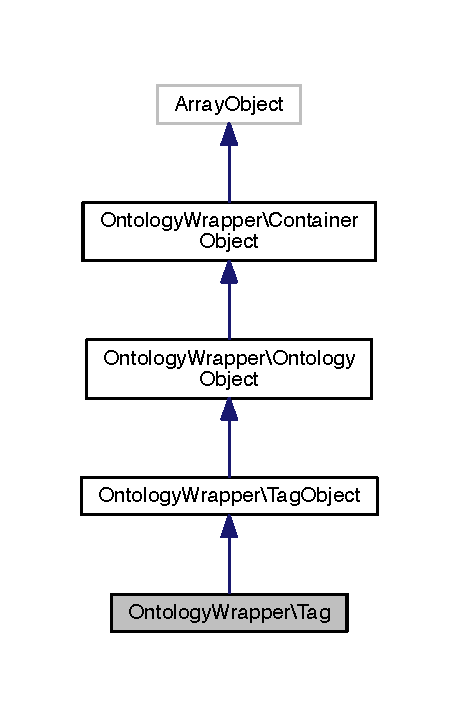
\includegraphics[width=220pt]{class_ontology_wrapper_1_1_tag__inherit__graph}
\end{center}
\end{figure}


Collaboration diagram for Ontology\-Wrapper\textbackslash{}Tag\-:
\nopagebreak
\begin{figure}[H]
\begin{center}
\leavevmode
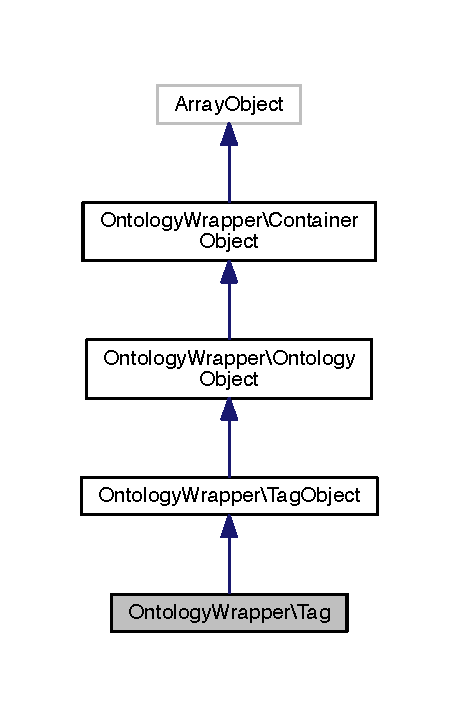
\includegraphics[width=220pt]{class_ontology_wrapper_1_1_tag__coll__graph}
\end{center}
\end{figure}
\subsection*{Public Member Functions}
\begin{DoxyCompactItemize}
\item 
\hyperlink{class_ontology_wrapper_1_1_tag_aa1e0088ed61d741f3679c3a3128007b1}{\-\_\-\-\_\-construct} (\$the\-Container=N\-U\-L\-L, \$the\-Identifier=N\-U\-L\-L)
\item 
\hyperlink{class_ontology_wrapper_1_1_tag_aa2e64f9c1b9f4cd55e5f31db154057b7}{load\-Terms} ()
\item 
\hyperlink{class_ontology_wrapper_1_1_tag_a8fafe8f4c5ac0208e0428a857d291103}{load\-Data\-Types} ()
\item 
\hyperlink{class_ontology_wrapper_1_1_tag_aaf0f041294cc04e07c0e92640e7544e7}{load\-Data\-Kinds} ()
\item 
\hyperlink{class_ontology_wrapper_1_1_tag_af565f8f24f7dff4ce1c3f40e9953345b}{collect\-References} (\&\$the\-Container, \$do\-Object=T\-R\-U\-E)
\end{DoxyCompactItemize}
\subsection*{Static Public Member Functions}
\begin{DoxyCompactItemize}
\item 
static \hyperlink{class_ontology_wrapper_1_1_tag_ab9e3d10fa0936027b6b0286b0cf77482}{Resolve\-Object} (\hyperlink{class_ontology_wrapper_1_1_connection_object}{Connection\-Object} \$the\-Connection, \$the\-Identifier, \$do\-Assert=T\-R\-U\-E)
\end{DoxyCompactItemize}
\subsection*{Public Attributes}
\begin{DoxyCompactItemize}
\item 
\hypertarget{class_ontology_wrapper_1_1_tag_aed2bdf74576154de4a2cbf7dfd5f9ea5}{const {\bfseries k\-S\-E\-Q\-\_\-\-N\-A\-M\-E} = '\-\_\-tags'}\label{class_ontology_wrapper_1_1_tag_aed2bdf74576154de4a2cbf7dfd5f9ea5}

\end{DoxyCompactItemize}
\subsection*{Protected Member Functions}
\begin{DoxyCompactItemize}
\item 
\hyperlink{class_ontology_wrapper_1_1_tag_a99ba84fc4fbbfc815dc60b2da6fd067d}{pre\-Commit} (\$the\-Operation=0x00)
\item 
\hyperlink{class_ontology_wrapper_1_1_tag_a6edfdc7fca0215a2456912f83893ef99}{post\-Commit} (\$the\-Operation=0x00)
\item 
\hyperlink{class_ontology_wrapper_1_1_tag_a43aac595d9e78147643e4c6136efa2b1}{is\-Ready} ()
\item 
\hyperlink{class_ontology_wrapper_1_1_tag_a9cc2af6aacbb8bbc52d4a4a641a2ae25}{post\-Offset\-Set} (\&\$the\-Offset, \&\$the\-Value)
\item 
\hyperlink{class_ontology_wrapper_1_1_tag_acdee636ad46bbe434fd47635a06d4495}{post\-Offset\-Unset} (\&\$the\-Offset)
\item 
\hyperlink{class_ontology_wrapper_1_1_tag_a191b408968b0d9bc9e8e2e8fadd24060}{locked\-Offsets} ()
\end{DoxyCompactItemize}
\subsection*{Additional Inherited Members}


\subsection{Detailed Description}
\hyperlink{class_ontology_wrapper_1_1_tag}{Tag}

This class implements a persistent \hyperlink{class_ontology_wrapper_1_1_tag_object}{Tag\-Object} instance, the class concentrates on implementing all the necessary elements to ensure persistence to instances of this class and referential integrity.

The object is considered initialised, \hyperlink{namespace_ontology_wrapper_a7c06300cb0043d3bab108f92cb9be3db}{is\-Inited()}, if it has at least the terms path, \hyperlink{}{k\-T\-A\-G\-\_\-\-T\-E\-R\-M\-S}, with an odd number of elements, the data type, \hyperlink{}{k\-T\-A\-G\-\_\-\-D\-A\-T\-A\-\_\-\-T\-Y\-P\-E}, and the label, \hyperlink{}{k\-T\-A\-G\-\_\-\-L\-A\-B\-E\-L}.

In this class we set the sequence number, \hyperlink{}{k\-T\-A\-G\-\_\-\-S\-E\-Q}, by retrieving a \begin{DoxyVerb} @author            Milko A. Škofič <m.skofic@cgiar.org>
 @version   1.00 07/02/2014\end{DoxyVerb}
 

\subsection{Constructor \& Destructor Documentation}
\hypertarget{class_ontology_wrapper_1_1_tag_aa1e0088ed61d741f3679c3a3128007b1}{\index{Ontology\-Wrapper\-::\-Tag@{Ontology\-Wrapper\-::\-Tag}!\-\_\-\-\_\-construct@{\-\_\-\-\_\-construct}}
\index{\-\_\-\-\_\-construct@{\-\_\-\-\_\-construct}!OntologyWrapper::Tag@{Ontology\-Wrapper\-::\-Tag}}
\subsubsection[{\-\_\-\-\_\-construct}]{\setlength{\rightskip}{0pt plus 5cm}Ontology\-Wrapper\textbackslash{}\-Tag\-::\-\_\-\-\_\-construct (
\begin{DoxyParamCaption}
\item[{}]{\$the\-Container = {\ttfamily NULL}, }
\item[{}]{\$the\-Identifier = {\ttfamily NULL}}
\end{DoxyParamCaption}
)}}\label{class_ontology_wrapper_1_1_tag_aa1e0088ed61d741f3679c3a3128007b1}
Instantiate class.

This constructor is standard for all persistent classes, we do nothing special here.


\begin{DoxyParams}[1]{Parameters}
\hyperlink{class_ontology_wrapper_1_1_connection_object}{Connection\-Object} & {\em \$the\-Container} & Persistent store. \\
\hline
mixed & {\em \$the\-Identifier} & Object identifier.\\
\hline
\end{DoxyParams}
public

\hyperlink{namespace_ontology_wrapper_ae6754181b2df357062755fcfe794a8b4}{instantiate\-Object()} 

\subsection{Member Function Documentation}
\hypertarget{class_ontology_wrapper_1_1_tag_af565f8f24f7dff4ce1c3f40e9953345b}{\index{Ontology\-Wrapper\-::\-Tag@{Ontology\-Wrapper\-::\-Tag}!collect\-References@{collect\-References}}
\index{collect\-References@{collect\-References}!OntologyWrapper::Tag@{Ontology\-Wrapper\-::\-Tag}}
\subsubsection[{collect\-References}]{\setlength{\rightskip}{0pt plus 5cm}Ontology\-Wrapper\textbackslash{}\-Tag\-::collect\-References (
\begin{DoxyParamCaption}
\item[{\&}]{\$the\-Container, }
\item[{}]{\$do\-Object = {\ttfamily TRUE}}
\end{DoxyParamCaption}
)}}\label{class_ontology_wrapper_1_1_tag_af565f8f24f7dff4ce1c3f40e9953345b}
Collect references

In this class we collect the terms list, the data types and the data kinds.


\begin{DoxyParams}[1]{Parameters}
reference & {\em \$the\-Container} & Receives objects. \\
\hline
boolean & {\em \$do\-Object} & {\ttfamily T\-R\-U\-E} load objects.\\
\hline
\end{DoxyParams}
public \hypertarget{class_ontology_wrapper_1_1_tag_a43aac595d9e78147643e4c6136efa2b1}{\index{Ontology\-Wrapper\-::\-Tag@{Ontology\-Wrapper\-::\-Tag}!is\-Ready@{is\-Ready}}
\index{is\-Ready@{is\-Ready}!OntologyWrapper::Tag@{Ontology\-Wrapper\-::\-Tag}}
\subsubsection[{is\-Ready}]{\setlength{\rightskip}{0pt plus 5cm}Ontology\-Wrapper\textbackslash{}\-Tag\-::is\-Ready (
\begin{DoxyParamCaption}
{}
\end{DoxyParamCaption}
)\hspace{0.3cm}{\ttfamily [protected]}}}\label{class_ontology_wrapper_1_1_tag_a43aac595d9e78147643e4c6136efa2b1}
Check if object is ready

In this class we ensure the object has the native identifier, \hyperlink{}{k\-T\-A\-G\-\_\-\-N\-I\-D}, the global identifier,  k\-T\-A\-G\-\_\-\-P\-I\-D\}, the data type, \hyperlink{}{k\-T\-A\-G\-\_\-\-D\-A\-T\-A\-\_\-\-T\-Y\-P\-E}, and the label, \hyperlink{}{k\-T\-A\-G\-\_\-\-L\-A\-B\-E\-L}.

protected \begin{DoxyReturn}{Returns}
Boolean {\ttfamily T\-R\-U\-E} means ready. 
\end{DoxyReturn}
\hypertarget{class_ontology_wrapper_1_1_tag_aaf0f041294cc04e07c0e92640e7544e7}{\index{Ontology\-Wrapper\-::\-Tag@{Ontology\-Wrapper\-::\-Tag}!load\-Data\-Kinds@{load\-Data\-Kinds}}
\index{load\-Data\-Kinds@{load\-Data\-Kinds}!OntologyWrapper::Tag@{Ontology\-Wrapper\-::\-Tag}}
\subsubsection[{load\-Data\-Kinds}]{\setlength{\rightskip}{0pt plus 5cm}Ontology\-Wrapper\textbackslash{}\-Tag\-::load\-Data\-Kinds (
\begin{DoxyParamCaption}
{}
\end{DoxyParamCaption}
)}}\label{class_ontology_wrapper_1_1_tag_aaf0f041294cc04e07c0e92640e7544e7}
Load data type objects list

This method can be used to resolve the list of data types into a list of objects.

The method will return an array, indexed by term native identifier, containing the resolved objects.

If any term cannot be resolved, the method will raise an exception.

protected \begin{DoxyReturn}{Returns}
array List of term objects or {\ttfamily N\-U\-L\-L}. 
\end{DoxyReturn}
\hypertarget{class_ontology_wrapper_1_1_tag_a8fafe8f4c5ac0208e0428a857d291103}{\index{Ontology\-Wrapper\-::\-Tag@{Ontology\-Wrapper\-::\-Tag}!load\-Data\-Types@{load\-Data\-Types}}
\index{load\-Data\-Types@{load\-Data\-Types}!OntologyWrapper::Tag@{Ontology\-Wrapper\-::\-Tag}}
\subsubsection[{load\-Data\-Types}]{\setlength{\rightskip}{0pt plus 5cm}Ontology\-Wrapper\textbackslash{}\-Tag\-::load\-Data\-Types (
\begin{DoxyParamCaption}
{}
\end{DoxyParamCaption}
)}}\label{class_ontology_wrapper_1_1_tag_a8fafe8f4c5ac0208e0428a857d291103}
Load data type objects list

This method can be used to resolve the list of data types into a list of objects.

The method will return an array, indexed by term native identifier, containing the resolved objects.

If any term cannot be resolved, the method will raise an exception.

protected \begin{DoxyReturn}{Returns}
array List of term objects or {\ttfamily N\-U\-L\-L}. 
\end{DoxyReturn}
\hypertarget{class_ontology_wrapper_1_1_tag_aa2e64f9c1b9f4cd55e5f31db154057b7}{\index{Ontology\-Wrapper\-::\-Tag@{Ontology\-Wrapper\-::\-Tag}!load\-Terms@{load\-Terms}}
\index{load\-Terms@{load\-Terms}!OntologyWrapper::Tag@{Ontology\-Wrapper\-::\-Tag}}
\subsubsection[{load\-Terms}]{\setlength{\rightskip}{0pt plus 5cm}Ontology\-Wrapper\textbackslash{}\-Tag\-::load\-Terms (
\begin{DoxyParamCaption}
{}
\end{DoxyParamCaption}
)}}\label{class_ontology_wrapper_1_1_tag_aa2e64f9c1b9f4cd55e5f31db154057b7}
Load term objects list

This method can be used to resolve the list of terms into a list of objects.

The method will return an array, indexed by term native identifier, containing the resolved objects.

If any term cannot be resolved, the method will raise an exception.

protected \begin{DoxyReturn}{Returns}
array List of term objects or {\ttfamily N\-U\-L\-L}. 
\end{DoxyReturn}
\hypertarget{class_ontology_wrapper_1_1_tag_a191b408968b0d9bc9e8e2e8fadd24060}{\index{Ontology\-Wrapper\-::\-Tag@{Ontology\-Wrapper\-::\-Tag}!locked\-Offsets@{locked\-Offsets}}
\index{locked\-Offsets@{locked\-Offsets}!OntologyWrapper::Tag@{Ontology\-Wrapper\-::\-Tag}}
\subsubsection[{locked\-Offsets}]{\setlength{\rightskip}{0pt plus 5cm}Ontology\-Wrapper\textbackslash{}\-Tag\-::locked\-Offsets (
\begin{DoxyParamCaption}
{}
\end{DoxyParamCaption}
)\hspace{0.3cm}{\ttfamily [protected]}}}\label{class_ontology_wrapper_1_1_tag_a191b408968b0d9bc9e8e2e8fadd24060}
Return list of locked offsets

In this class we return the static \hyperlink{}{\$s\-Internal\-Tags} list, the \hyperlink{}{k\-T\-A\-G\-\_\-\-P\-I\-D}, \hyperlink{}{k\-T\-A\-G\-\_\-\-S\-E\-Q}, \hyperlink{}{k\-T\-A\-G\-\_\-\-T\-E\-R\-M\-S}, \hyperlink{}{k\-T\-A\-G\-\_\-\-D\-A\-T\-A\-\_\-\-T\-Y\-P\-E} and the \hyperlink{}{k\-T\-A\-G\-\_\-\-D\-A\-T\-A\-\_\-\-K\-I\-N\-D} offsets.

protected \begin{DoxyReturn}{Returns}
array List of locked offsets.
\end{DoxyReturn}
\begin{DoxySeeAlso}{See Also}
k\-T\-A\-G\-\_\-\-S\-E\-Q k\-T\-A\-G\-\_\-\-T\-E\-R\-M\-S k\-T\-A\-G\-\_\-\-D\-A\-T\-A\-\_\-\-T\-Y\-P\-E k\-T\-A\-G\-\_\-\-D\-A\-T\-A\-\_\-\-K\-I\-N\-D 
\end{DoxySeeAlso}
\hypertarget{class_ontology_wrapper_1_1_tag_a6edfdc7fca0215a2456912f83893ef99}{\index{Ontology\-Wrapper\-::\-Tag@{Ontology\-Wrapper\-::\-Tag}!post\-Commit@{post\-Commit}}
\index{post\-Commit@{post\-Commit}!OntologyWrapper::Tag@{Ontology\-Wrapper\-::\-Tag}}
\subsubsection[{post\-Commit}]{\setlength{\rightskip}{0pt plus 5cm}Ontology\-Wrapper\textbackslash{}\-Tag\-::post\-Commit (
\begin{DoxyParamCaption}
\item[{}]{\$the\-Operation = {\ttfamily 0x00}}
\end{DoxyParamCaption}
)\hspace{0.3cm}{\ttfamily [protected]}}}\label{class_ontology_wrapper_1_1_tag_a6edfdc7fca0215a2456912f83893ef99}
Cleanup object after commit

In this class we set the newly inserted or updated tag into the cache, or delete it from the cache if deleting.


\begin{DoxyParams}[1]{Parameters}
bitfield & {\em \$the\-Operation} & Operation code.\\
\hline
\end{DoxyParams}
protected \hypertarget{class_ontology_wrapper_1_1_tag_a9cc2af6aacbb8bbc52d4a4a641a2ae25}{\index{Ontology\-Wrapper\-::\-Tag@{Ontology\-Wrapper\-::\-Tag}!post\-Offset\-Set@{post\-Offset\-Set}}
\index{post\-Offset\-Set@{post\-Offset\-Set}!OntologyWrapper::Tag@{Ontology\-Wrapper\-::\-Tag}}
\subsubsection[{post\-Offset\-Set}]{\setlength{\rightskip}{0pt plus 5cm}Ontology\-Wrapper\textbackslash{}\-Tag\-::post\-Offset\-Set (
\begin{DoxyParamCaption}
\item[{\&}]{\$the\-Offset, }
\item[{\&}]{\$the\-Value}
\end{DoxyParamCaption}
)\hspace{0.3cm}{\ttfamily [protected]}}}\label{class_ontology_wrapper_1_1_tag_a9cc2af6aacbb8bbc52d4a4a641a2ae25}
Handle offset and value after setting it

In this class we set the \hyperlink{namespace_ontology_wrapper_a7c06300cb0043d3bab108f92cb9be3db}{is\-Inited()} status.


\begin{DoxyParams}[1]{Parameters}
reference & {\em \$the\-Offset} & Offset reference. \\
\hline
reference & {\em \$the\-Value} & Offset value reference.\\
\hline
\end{DoxyParams}
protected

\begin{DoxySeeAlso}{See Also}
k\-T\-A\-G\-\_\-\-T\-E\-R\-M\-S k\-T\-A\-G\-\_\-\-D\-A\-T\-A\-\_\-\-T\-Y\-P\-E k\-T\-A\-G\-\_\-\-L\-A\-B\-E\-L 
\end{DoxySeeAlso}
\hypertarget{class_ontology_wrapper_1_1_tag_acdee636ad46bbe434fd47635a06d4495}{\index{Ontology\-Wrapper\-::\-Tag@{Ontology\-Wrapper\-::\-Tag}!post\-Offset\-Unset@{post\-Offset\-Unset}}
\index{post\-Offset\-Unset@{post\-Offset\-Unset}!OntologyWrapper::Tag@{Ontology\-Wrapper\-::\-Tag}}
\subsubsection[{post\-Offset\-Unset}]{\setlength{\rightskip}{0pt plus 5cm}Ontology\-Wrapper\textbackslash{}\-Tag\-::post\-Offset\-Unset (
\begin{DoxyParamCaption}
\item[{\&}]{\$the\-Offset}
\end{DoxyParamCaption}
)\hspace{0.3cm}{\ttfamily [protected]}}}\label{class_ontology_wrapper_1_1_tag_acdee636ad46bbe434fd47635a06d4495}
Handle offset after deleting it

In this class we set the \hyperlink{namespace_ontology_wrapper_a7c06300cb0043d3bab108f92cb9be3db}{is\-Inited()} status.


\begin{DoxyParams}[1]{Parameters}
reference & {\em \$the\-Offset} & Offset reference.\\
\hline
\end{DoxyParams}
protected

\begin{DoxySeeAlso}{See Also}
k\-T\-A\-G\-\_\-\-D\-A\-T\-A\-\_\-\-T\-Y\-P\-E k\-T\-A\-G\-\_\-\-L\-A\-B\-E\-L 
\end{DoxySeeAlso}
\hypertarget{class_ontology_wrapper_1_1_tag_a99ba84fc4fbbfc815dc60b2da6fd067d}{\index{Ontology\-Wrapper\-::\-Tag@{Ontology\-Wrapper\-::\-Tag}!pre\-Commit@{pre\-Commit}}
\index{pre\-Commit@{pre\-Commit}!OntologyWrapper::Tag@{Ontology\-Wrapper\-::\-Tag}}
\subsubsection[{pre\-Commit}]{\setlength{\rightskip}{0pt plus 5cm}Ontology\-Wrapper\textbackslash{}\-Tag\-::pre\-Commit (
\begin{DoxyParamCaption}
\item[{}]{\$the\-Operation = {\ttfamily 0x00}}
\end{DoxyParamCaption}
)\hspace{0.3cm}{\ttfamily [protected]}}}\label{class_ontology_wrapper_1_1_tag_a99ba84fc4fbbfc815dc60b2da6fd067d}
Prepare object for commit

In this class we first check if the object is \hyperlink{namespace_ontology_wrapper_a7c06300cb0043d3bab108f92cb9be3db}{is\-Inited()}, if that is not the case, we raise an exception, since the object cannot be committed if not initialised.

We then set the native identifier, if not yet filled, with the global identifier generated by the \hyperlink{class_ontology_wrapper_1_1_tag_object_aa942610424d0d9ccd25f77fa2d5ac175}{\-\_\-\-\_\-to\-String()} method.

We finally set the sequence number, \hyperlink{}{k\-T\-A\-G\-\_\-\-S\-E\-Q}, if it is not yet set by requesting it from the database of the current object's container.

When deleting we check whether the object has its native identifier.


\begin{DoxyParams}[1]{Parameters}
bitfield & {\em \$the\-Operation} & Operation code.\\
\hline
\end{DoxyParams}
protected

Exception \hypertarget{class_ontology_wrapper_1_1_tag_ab9e3d10fa0936027b6b0286b0cf77482}{\index{Ontology\-Wrapper\-::\-Tag@{Ontology\-Wrapper\-::\-Tag}!Resolve\-Object@{Resolve\-Object}}
\index{Resolve\-Object@{Resolve\-Object}!OntologyWrapper::Tag@{Ontology\-Wrapper\-::\-Tag}}
\subsubsection[{Resolve\-Object}]{\setlength{\rightskip}{0pt plus 5cm}static Ontology\-Wrapper\textbackslash{}\-Tag\-::\-Resolve\-Object (
\begin{DoxyParamCaption}
\item[{{\bf Connection\-Object}}]{\$the\-Connection, }
\item[{}]{\$the\-Identifier, }
\item[{}]{\$do\-Assert = {\ttfamily TRUE}}
\end{DoxyParamCaption}
)\hspace{0.3cm}{\ttfamily [static]}}}\label{class_ontology_wrapper_1_1_tag_ab9e3d10fa0936027b6b0286b0cf77482}
Resolve object

This method can be used to statically instantiate an object from the provided data store, it will attempt to select the object matching the provided native identifier and return an instance of the originally committed class.

The method accepts the following parameters\-:


\begin{DoxyItemize}
\item {\bfseries \$the\-Container}\-: The database or collection from which the object is to be retrieved. 
\item {\bfseries \$the\-Identifier}\-: The objet native identifier or sequence number. 
\item {\bfseries \$do\-Assert}\-: If {\ttfamily T\-R\-U\-E}, if the object is not matched, the method will raise an exception; if {\ttfamily F\-A\-L\-S\-E}, the method will return {\ttfamily N\-U\-L\-L}. 
\end{DoxyItemize}

We implement this method to match objects in the tags collection by matching string identifiers with the native identifier and integer identifiers with the sequence number.


\begin{DoxyParams}[1]{Parameters}
\hyperlink{class_ontology_wrapper_1_1_connection_object}{Connection\-Object} & {\em \$the\-Connection} & Persistent store. \\
\hline
mixed & {\em \$the\-Identifier} & Object identifier. \\
\hline
boolean & {\em \$do\-Assert} & Assert object.\\
\hline
\end{DoxyParams}
public \begin{DoxyReturn}{Returns}
\hyperlink{class_ontology_wrapper_1_1_ontology_object}{Ontology\-Object} Object or {\ttfamily N\-U\-L\-L}. 
\end{DoxyReturn}


The documentation for this class was generated from the following file\-:\begin{DoxyCompactItemize}
\item 
/\-Library/\-Web\-Server/\-Library/\-Ontology\-Wrapper/\-Library/\-Ontology\-Wrapper/Tag.\-php\end{DoxyCompactItemize}

\hypertarget{class_ontology_wrapper_1_1_term}{\section{Ontology\-Wrapper\textbackslash{}Term Class Reference}
\label{class_ontology_wrapper_1_1_term}\index{Ontology\-Wrapper\textbackslash{}\-Term@{Ontology\-Wrapper\textbackslash{}\-Term}}
}


Inheritance diagram for Ontology\-Wrapper\textbackslash{}Term\-:
\nopagebreak
\begin{figure}[H]
\begin{center}
\leavevmode
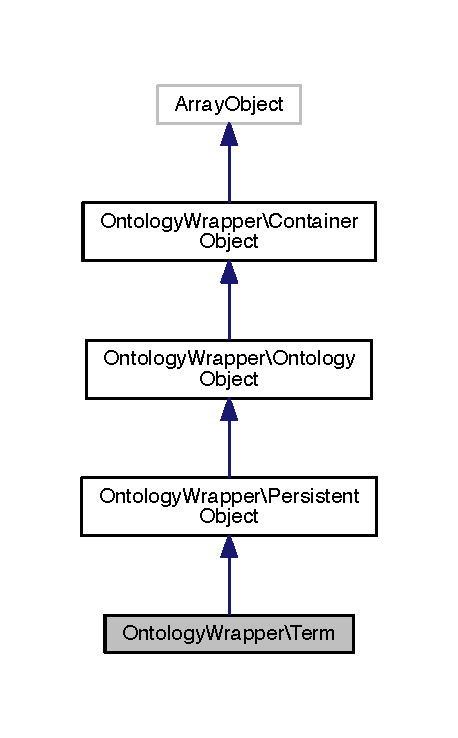
\includegraphics[width=228pt]{class_ontology_wrapper_1_1_term__inherit__graph}
\end{center}
\end{figure}


Collaboration diagram for Ontology\-Wrapper\textbackslash{}Term\-:
\nopagebreak
\begin{figure}[H]
\begin{center}
\leavevmode
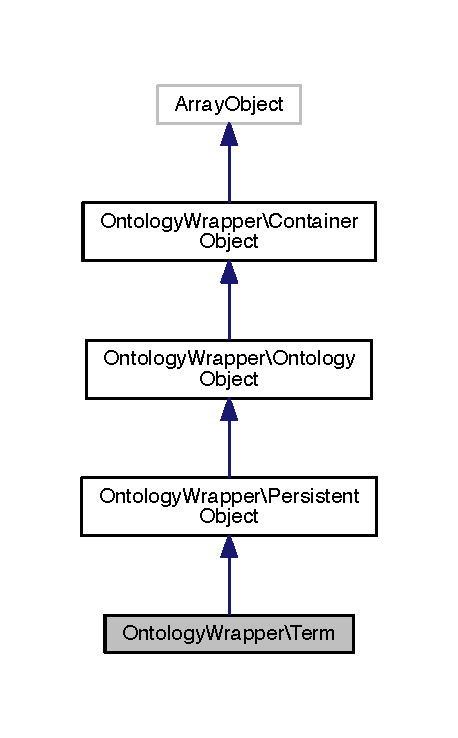
\includegraphics[width=228pt]{class_ontology_wrapper_1_1_term__coll__graph}
\end{center}
\end{figure}
\subsection*{Public Member Functions}
\begin{DoxyCompactItemize}
\item 
\hyperlink{class_ontology_wrapper_1_1_term_af15064bcbdb083627b156deb9bce7aea}{\-\_\-\-\_\-construct} (\$the\-Container=N\-U\-L\-L, \$the\-Identifier=N\-U\-L\-L)
\item 
\hyperlink{class_ontology_wrapper_1_1_term_aff4bc870850271310f116c433999a3c5}{load\-Namespace} ()
\item 
\hyperlink{class_ontology_wrapper_1_1_term_a9247b063058e8cdbe94a8a774a70e70e}{collect\-References} (\&\$the\-Container, \$do\-Object=T\-R\-U\-E)
\end{DoxyCompactItemize}
\subsection*{Static Public Member Functions}
\begin{DoxyCompactItemize}
\item 
static \hyperlink{class_ontology_wrapper_1_1_term_a752e5172e2c51dcf9aaf24f49139ec80}{Resolve\-Object} (\hyperlink{class_ontology_wrapper_1_1_connection_object}{Connection\-Object} \$the\-Connection, \$the\-Identifier, \$do\-Assert=T\-R\-U\-E)
\end{DoxyCompactItemize}
\subsection*{Public Attributes}
\begin{DoxyCompactItemize}
\item 
\hypertarget{class_ontology_wrapper_1_1_term_a5731878c2b563dbc2be121ba29fa7086}{const {\bfseries k\-S\-E\-Q\-\_\-\-N\-A\-M\-E} = '\-\_\-terms'}\label{class_ontology_wrapper_1_1_term_a5731878c2b563dbc2be121ba29fa7086}

\end{DoxyCompactItemize}
\subsection*{Protected Member Functions}
\begin{DoxyCompactItemize}
\item 
\hyperlink{class_ontology_wrapper_1_1_term_a765f0bc982832d1b6dd3732a1c5ef643}{pre\-Commit} (\$the\-Operation=0x00)
\item 
\hyperlink{class_ontology_wrapper_1_1_term_a8db3eede1845e4c53f9aa1a49cb8c719}{post\-Commit} (\$the\-Operation=0x00)
\item 
\hyperlink{class_ontology_wrapper_1_1_term_ae1c796d23d15f49b132025b268c5763b}{is\-Ready} ()
\item 
\hyperlink{class_ontology_wrapper_1_1_term_aa59636200bca2de1b23380a6376f65df}{post\-Offset\-Set} (\&\$the\-Offset, \&\$the\-Value)
\item 
\hyperlink{class_ontology_wrapper_1_1_term_af6d43299cf5932b581548aaf5a8515d9}{post\-Offset\-Unset} (\&\$the\-Offset)
\item 
\hyperlink{class_ontology_wrapper_1_1_term_a174e341c129088cdc8b845e0176d6eb4}{locked\-Offsets} ()
\end{DoxyCompactItemize}
\subsection*{Additional Inherited Members}


\subsection{Detailed Description}
\hyperlink{class_ontology_wrapper_1_1_term}{Term}

This class implements a persistent \hyperlink{class_ontology_wrapper_1_1_term_object}{Term\-Object} instance, the class concentrates on implementing all the necessary elements to ensure persistence to instances of this class and referential integrity.

The object is considered initialised, \hyperlink{namespace_ontology_wrapper_a7c06300cb0043d3bab108f92cb9be3db}{is\-Inited()}, if it has at least the local identifier, \hyperlink{}{k\-T\-A\-G\-\_\-\-L\-I\-D}, and the label, \hyperlink{}{k\-T\-A\-G\-\_\-\-L\-A\-B\-E\-L}. \begin{DoxyVerb} @author            Milko A. Škofič <m.skofic@cgiar.org>
 @version   1.00 07/02/2014\end{DoxyVerb}
 

\subsection{Constructor \& Destructor Documentation}
\hypertarget{class_ontology_wrapper_1_1_term_af15064bcbdb083627b156deb9bce7aea}{\index{Ontology\-Wrapper\-::\-Term@{Ontology\-Wrapper\-::\-Term}!\-\_\-\-\_\-construct@{\-\_\-\-\_\-construct}}
\index{\-\_\-\-\_\-construct@{\-\_\-\-\_\-construct}!OntologyWrapper::Term@{Ontology\-Wrapper\-::\-Term}}
\subsubsection[{\-\_\-\-\_\-construct}]{\setlength{\rightskip}{0pt plus 5cm}Ontology\-Wrapper\textbackslash{}\-Term\-::\-\_\-\-\_\-construct (
\begin{DoxyParamCaption}
\item[{}]{\$the\-Container = {\ttfamily NULL}, }
\item[{}]{\$the\-Identifier = {\ttfamily NULL}}
\end{DoxyParamCaption}
)}}\label{class_ontology_wrapper_1_1_term_af15064bcbdb083627b156deb9bce7aea}
Instantiate class.

This constructor is standard for all persistent classes, we do nothing special here.


\begin{DoxyParams}[1]{Parameters}
\hyperlink{class_ontology_wrapper_1_1_connection_object}{Connection\-Object} & {\em \$the\-Container} & Persistent store. \\
\hline
mixed & {\em \$the\-Identifier} & Object identifier.\\
\hline
\end{DoxyParams}
public

\hyperlink{namespace_ontology_wrapper_ae6754181b2df357062755fcfe794a8b4}{instantiate\-Object()} 

\subsection{Member Function Documentation}
\hypertarget{class_ontology_wrapper_1_1_term_a9247b063058e8cdbe94a8a774a70e70e}{\index{Ontology\-Wrapper\-::\-Term@{Ontology\-Wrapper\-::\-Term}!collect\-References@{collect\-References}}
\index{collect\-References@{collect\-References}!OntologyWrapper::Term@{Ontology\-Wrapper\-::\-Term}}
\subsubsection[{collect\-References}]{\setlength{\rightskip}{0pt plus 5cm}Ontology\-Wrapper\textbackslash{}\-Term\-::collect\-References (
\begin{DoxyParamCaption}
\item[{\&}]{\$the\-Container, }
\item[{}]{\$do\-Object = {\ttfamily TRUE}}
\end{DoxyParamCaption}
)}}\label{class_ontology_wrapper_1_1_term_a9247b063058e8cdbe94a8a774a70e70e}
Collect references

In this class we collect the namespace.


\begin{DoxyParams}[1]{Parameters}
reference & {\em \$the\-Container} & Receives objects. \\
\hline
boolean & {\em \$do\-Object} & {\ttfamily T\-R\-U\-E} load objects.\\
\hline
\end{DoxyParams}
public \hypertarget{class_ontology_wrapper_1_1_term_ae1c796d23d15f49b132025b268c5763b}{\index{Ontology\-Wrapper\-::\-Term@{Ontology\-Wrapper\-::\-Term}!is\-Ready@{is\-Ready}}
\index{is\-Ready@{is\-Ready}!OntologyWrapper::Term@{Ontology\-Wrapper\-::\-Term}}
\subsubsection[{is\-Ready}]{\setlength{\rightskip}{0pt plus 5cm}Ontology\-Wrapper\textbackslash{}\-Term\-::is\-Ready (
\begin{DoxyParamCaption}
{}
\end{DoxyParamCaption}
)\hspace{0.3cm}{\ttfamily [protected]}}}\label{class_ontology_wrapper_1_1_term_ae1c796d23d15f49b132025b268c5763b}
Check if object is ready

In this class we ensure the object has the native identifier, \hyperlink{}{k\-T\-A\-G\-\_\-\-N\-I\-D}, the global identifier,  k\-T\-A\-G\-\_\-\-P\-I\-D\}, the data type, \hyperlink{}{k\-T\-A\-G\-\_\-\-D\-A\-T\-A\-\_\-\-T\-Y\-P\-E}, and the label, \hyperlink{}{k\-T\-A\-G\-\_\-\-L\-A\-B\-E\-L}.

protected \begin{DoxyReturn}{Returns}
Boolean {\ttfamily T\-R\-U\-E} means ready. 
\end{DoxyReturn}
\hypertarget{class_ontology_wrapper_1_1_term_aff4bc870850271310f116c433999a3c5}{\index{Ontology\-Wrapper\-::\-Term@{Ontology\-Wrapper\-::\-Term}!load\-Namespace@{load\-Namespace}}
\index{load\-Namespace@{load\-Namespace}!OntologyWrapper::Term@{Ontology\-Wrapper\-::\-Term}}
\subsubsection[{load\-Namespace}]{\setlength{\rightskip}{0pt plus 5cm}Ontology\-Wrapper\textbackslash{}\-Term\-::load\-Namespace (
\begin{DoxyParamCaption}
{}
\end{DoxyParamCaption}
)}}\label{class_ontology_wrapper_1_1_term_aff4bc870850271310f116c433999a3c5}
Load namespace object

This method can be used to resolve the namespace into an object.

The method will return the namespace object if the operation succeeded and {\ttfamily N\-U\-L\-L} if the object is not committed, if the object does not hold a collection reference, or if the object has no namespace.

If the namespace cannot be resolved, the method will raise an exception.

protected \begin{DoxyReturn}{Returns}
\hyperlink{class_ontology_wrapper_1_1_term}{Term} Resolved reference or {\ttfamily N\-U\-L\-L}. 
\end{DoxyReturn}
\hypertarget{class_ontology_wrapper_1_1_term_a174e341c129088cdc8b845e0176d6eb4}{\index{Ontology\-Wrapper\-::\-Term@{Ontology\-Wrapper\-::\-Term}!locked\-Offsets@{locked\-Offsets}}
\index{locked\-Offsets@{locked\-Offsets}!OntologyWrapper::Term@{Ontology\-Wrapper\-::\-Term}}
\subsubsection[{locked\-Offsets}]{\setlength{\rightskip}{0pt plus 5cm}Ontology\-Wrapper\textbackslash{}\-Term\-::locked\-Offsets (
\begin{DoxyParamCaption}
{}
\end{DoxyParamCaption}
)\hspace{0.3cm}{\ttfamily [protected]}}}\label{class_ontology_wrapper_1_1_term_a174e341c129088cdc8b845e0176d6eb4}
Return list of locked offsets

In this class we return the static \hyperlink{}{\$s\-Internal\-Tags} list, the \hyperlink{}{k\-T\-A\-G\-\_\-\-P\-I\-D}, \hyperlink{}{k\-T\-A\-G\-\_\-\-N\-S} and the \hyperlink{}{k\-T\-A\-G\-\_\-\-L\-I\-D} offsets.

protected \begin{DoxyReturn}{Returns}
array List of locked offsets.
\end{DoxyReturn}
\begin{DoxySeeAlso}{See Also}
k\-T\-A\-G\-\_\-\-N\-S k\-T\-A\-G\-\_\-\-L\-I\-D 
\end{DoxySeeAlso}
\hypertarget{class_ontology_wrapper_1_1_term_a8db3eede1845e4c53f9aa1a49cb8c719}{\index{Ontology\-Wrapper\-::\-Term@{Ontology\-Wrapper\-::\-Term}!post\-Commit@{post\-Commit}}
\index{post\-Commit@{post\-Commit}!OntologyWrapper::Term@{Ontology\-Wrapper\-::\-Term}}
\subsubsection[{post\-Commit}]{\setlength{\rightskip}{0pt plus 5cm}Ontology\-Wrapper\textbackslash{}\-Term\-::post\-Commit (
\begin{DoxyParamCaption}
\item[{}]{\$the\-Operation = {\ttfamily 0x00}}
\end{DoxyParamCaption}
)\hspace{0.3cm}{\ttfamily [protected]}}}\label{class_ontology_wrapper_1_1_term_a8db3eede1845e4c53f9aa1a49cb8c719}
Cleanup object after commit

In this class we do nothing... yet.


\begin{DoxyParams}[1]{Parameters}
bitfield & {\em \$the\-Operation} & Operation code.\\
\hline
\end{DoxyParams}
protected \hypertarget{class_ontology_wrapper_1_1_term_aa59636200bca2de1b23380a6376f65df}{\index{Ontology\-Wrapper\-::\-Term@{Ontology\-Wrapper\-::\-Term}!post\-Offset\-Set@{post\-Offset\-Set}}
\index{post\-Offset\-Set@{post\-Offset\-Set}!OntologyWrapper::Term@{Ontology\-Wrapper\-::\-Term}}
\subsubsection[{post\-Offset\-Set}]{\setlength{\rightskip}{0pt plus 5cm}Ontology\-Wrapper\textbackslash{}\-Term\-::post\-Offset\-Set (
\begin{DoxyParamCaption}
\item[{\&}]{\$the\-Offset, }
\item[{\&}]{\$the\-Value}
\end{DoxyParamCaption}
)\hspace{0.3cm}{\ttfamily [protected]}}}\label{class_ontology_wrapper_1_1_term_aa59636200bca2de1b23380a6376f65df}
Handle offset and value after setting it

In this class we set the \hyperlink{namespace_ontology_wrapper_a7c06300cb0043d3bab108f92cb9be3db}{is\-Inited()} status.


\begin{DoxyParams}[1]{Parameters}
reference & {\em \$the\-Offset} & Offset reference. \\
\hline
reference & {\em \$the\-Value} & Offset value reference.\\
\hline
\end{DoxyParams}
protected

\begin{DoxySeeAlso}{See Also}
k\-T\-A\-G\-\_\-\-L\-I\-D k\-T\-A\-G\-\_\-\-L\-A\-B\-E\-L 
\end{DoxySeeAlso}
\hypertarget{class_ontology_wrapper_1_1_term_af6d43299cf5932b581548aaf5a8515d9}{\index{Ontology\-Wrapper\-::\-Term@{Ontology\-Wrapper\-::\-Term}!post\-Offset\-Unset@{post\-Offset\-Unset}}
\index{post\-Offset\-Unset@{post\-Offset\-Unset}!OntologyWrapper::Term@{Ontology\-Wrapper\-::\-Term}}
\subsubsection[{post\-Offset\-Unset}]{\setlength{\rightskip}{0pt plus 5cm}Ontology\-Wrapper\textbackslash{}\-Term\-::post\-Offset\-Unset (
\begin{DoxyParamCaption}
\item[{\&}]{\$the\-Offset}
\end{DoxyParamCaption}
)\hspace{0.3cm}{\ttfamily [protected]}}}\label{class_ontology_wrapper_1_1_term_af6d43299cf5932b581548aaf5a8515d9}
Handle offset after deleting it

In this class we set the \hyperlink{namespace_ontology_wrapper_a7c06300cb0043d3bab108f92cb9be3db}{is\-Inited()} status.


\begin{DoxyParams}[1]{Parameters}
reference & {\em \$the\-Offset} & Offset reference.\\
\hline
\end{DoxyParams}
protected

\begin{DoxySeeAlso}{See Also}
k\-T\-A\-G\-\_\-\-L\-I\-D k\-T\-A\-G\-\_\-\-L\-A\-B\-E\-L 
\end{DoxySeeAlso}
\hypertarget{class_ontology_wrapper_1_1_term_a765f0bc982832d1b6dd3732a1c5ef643}{\index{Ontology\-Wrapper\-::\-Term@{Ontology\-Wrapper\-::\-Term}!pre\-Commit@{pre\-Commit}}
\index{pre\-Commit@{pre\-Commit}!OntologyWrapper::Term@{Ontology\-Wrapper\-::\-Term}}
\subsubsection[{pre\-Commit}]{\setlength{\rightskip}{0pt plus 5cm}Ontology\-Wrapper\textbackslash{}\-Term\-::pre\-Commit (
\begin{DoxyParamCaption}
\item[{}]{\$the\-Operation = {\ttfamily 0x00}}
\end{DoxyParamCaption}
)\hspace{0.3cm}{\ttfamily [protected]}}}\label{class_ontology_wrapper_1_1_term_a765f0bc982832d1b6dd3732a1c5ef643}
Prepare object for commit

In this class we first check if the object is \hyperlink{namespace_ontology_wrapper_a7c06300cb0043d3bab108f92cb9be3db}{is\-Inited()}, if that is not the case, we raise an exception, since the object cannot be committed if not initialised.

We then set the native identifier, if not yet filled, with the global identifier generated by the \hyperlink{class_ontology_wrapper_1_1_term_object_a31dc54e3b2e1993f347a15314c071c5a}{\-\_\-\-\_\-to\-String()} method.

When deleting we check whether the object has its native identifier.


\begin{DoxyParams}[1]{Parameters}
bitfield & {\em \$the\-Operation} & Operation code.\\
\hline
\end{DoxyParams}
protected

Exception \hypertarget{class_ontology_wrapper_1_1_term_a752e5172e2c51dcf9aaf24f49139ec80}{\index{Ontology\-Wrapper\-::\-Term@{Ontology\-Wrapper\-::\-Term}!Resolve\-Object@{Resolve\-Object}}
\index{Resolve\-Object@{Resolve\-Object}!OntologyWrapper::Term@{Ontology\-Wrapper\-::\-Term}}
\subsubsection[{Resolve\-Object}]{\setlength{\rightskip}{0pt plus 5cm}static Ontology\-Wrapper\textbackslash{}\-Term\-::\-Resolve\-Object (
\begin{DoxyParamCaption}
\item[{{\bf Connection\-Object}}]{\$the\-Connection, }
\item[{}]{\$the\-Identifier, }
\item[{}]{\$do\-Assert = {\ttfamily TRUE}}
\end{DoxyParamCaption}
)\hspace{0.3cm}{\ttfamily [static]}}}\label{class_ontology_wrapper_1_1_term_a752e5172e2c51dcf9aaf24f49139ec80}
Resolve object

This method can be used to statically instantiate an object from the provided data store, it will attempt to select the object matching the provided native identifier and return an instance of the originally committed class.

The method accepts the following parameters\-:


\begin{DoxyItemize}
\item {\bfseries \$the\-Container}\-: The database or collection from which the object is to be retrieved. 
\item {\bfseries \$the\-Identifier}\-: The objet native identifier. 
\item {\bfseries \$do\-Assert}\-: If {\ttfamily T\-R\-U\-E}, if the object is not matched, the method will raise an exception; if {\ttfamily F\-A\-L\-S\-E}, the method will return {\ttfamily N\-U\-L\-L}. 
\end{DoxyItemize}

We implement this method to match objects in the terms collection.


\begin{DoxyParams}[1]{Parameters}
\hyperlink{class_ontology_wrapper_1_1_connection_object}{Connection\-Object} & {\em \$the\-Connection} & Persistent store. \\
\hline
mixed & {\em \$the\-Identifier} & Object identifier. \\
\hline
boolean & {\em \$do\-Assert} & Assert object.\\
\hline
\end{DoxyParams}
public \begin{DoxyReturn}{Returns}
\hyperlink{class_ontology_wrapper_1_1_ontology_object}{Ontology\-Object} Object or {\ttfamily N\-U\-L\-L}. 
\end{DoxyReturn}


The documentation for this class was generated from the following file\-:\begin{DoxyCompactItemize}
\item 
/\-Library/\-Web\-Server/\-Library/\-Ontology\-Wrapper/\-Library/\-Ontology\-Wrapper/Term.\-php\end{DoxyCompactItemize}

\hypertarget{class_ontology_wrapper_1_1_wrapper}{\section{Ontology\-Wrapper\textbackslash{}Wrapper Class Reference}
\label{class_ontology_wrapper_1_1_wrapper}\index{Ontology\-Wrapper\textbackslash{}\-Wrapper@{Ontology\-Wrapper\textbackslash{}\-Wrapper}}
}


Inheritance diagram for Ontology\-Wrapper\textbackslash{}Wrapper\-:
\nopagebreak
\begin{figure}[H]
\begin{center}
\leavevmode
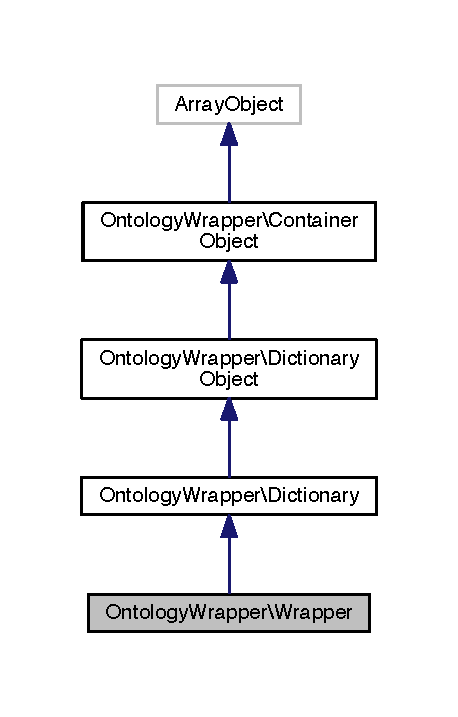
\includegraphics[width=220pt]{class_ontology_wrapper_1_1_wrapper__inherit__graph}
\end{center}
\end{figure}


Collaboration diagram for Ontology\-Wrapper\textbackslash{}Wrapper\-:
\nopagebreak
\begin{figure}[H]
\begin{center}
\leavevmode
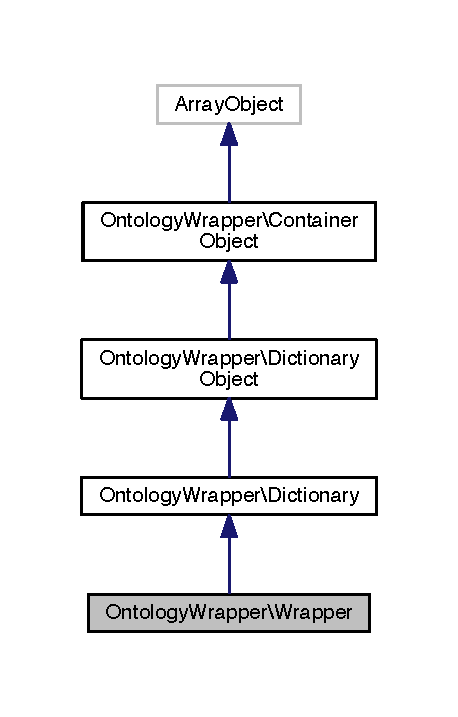
\includegraphics[width=220pt]{class_ontology_wrapper_1_1_wrapper__coll__graph}
\end{center}
\end{figure}
\subsection*{Public Member Functions}
\begin{DoxyCompactItemize}
\item 
\hyperlink{class_ontology_wrapper_1_1_wrapper_a58530473d4c2b9847a72b4568c7c52bb}{Metadata} (\$the\-Value=N\-U\-L\-L, \$get\-Old=F\-A\-L\-S\-E)
\item 
\hyperlink{class_ontology_wrapper_1_1_wrapper_aa3446362c7c65332a05e53546dbc7ea2}{Entities} (\$the\-Value=N\-U\-L\-L, \$get\-Old=F\-A\-L\-S\-E)
\item 
\hyperlink{class_ontology_wrapper_1_1_wrapper_a04c8c36bebf40208956e797b5dc64fec}{Units} (\$the\-Value=N\-U\-L\-L, \$get\-Old=F\-A\-L\-S\-E)
\item 
\hyperlink{class_ontology_wrapper_1_1_wrapper_a94bab4d3e13b169479d5a0f9d16ea3fc}{is\-Connected} ()
\item 
\hyperlink{class_ontology_wrapper_1_1_wrapper_ae402cf57a8c037c3fe580baa252e99ac}{open\-Connections} ()
\item 
\hyperlink{class_ontology_wrapper_1_1_wrapper_a41ab06d375f9baae6349b4955ab8384e}{close\-Connections} ()
\item 
\hyperlink{class_ontology_wrapper_1_1_wrapper_a386b16160195cbb9c60d858b5677c1b4}{reset\-Ontology} ()
\item 
\hyperlink{class_ontology_wrapper_1_1_wrapper_ae03422dc6a2e5f5e03726b85f62a1f12}{load\-Tag\-Cache} ()
\item 
\hyperlink{class_ontology_wrapper_1_1_wrapper_a2ee823f34e78d0a1f2361d6da3f58532}{load\-X\-M\-L\-File} (\$the\-File)
\end{DoxyCompactItemize}
\subsection*{Protected Member Functions}
\begin{DoxyCompactItemize}
\item 
\hyperlink{class_ontology_wrapper_1_1_wrapper_aa8b5ac231784ffcda74ea463c6e92cc1}{load\-X\-M\-L\-Metadata} (\textbackslash{}Simple\-X\-M\-L\-Element \$the\-X\-M\-L)
\item 
\hyperlink{class_ontology_wrapper_1_1_wrapper_adbb3bf1090ccdf7ed89ffd494a0b101c}{load\-X\-M\-L\-Entities} (\textbackslash{}Simple\-X\-M\-L\-Element \$the\-X\-M\-L)
\item 
\hyperlink{class_ontology_wrapper_1_1_wrapper_aaad33b2f3f398545a234f7650f126321}{load\-X\-M\-L\-Units} (\textbackslash{}Simple\-X\-M\-L\-Element \$the\-X\-M\-L)
\item 
\hyperlink{class_ontology_wrapper_1_1_wrapper_a3500af2ce8421aed6b1f6dcfb5112546}{load\-X\-M\-L\-Metadata\-Block} (\textbackslash{}Simple\-X\-M\-L\-Element \$the\-X\-M\-L)
\item 
\hyperlink{class_ontology_wrapper_1_1_wrapper_a14c77bdeec16286c776ebe375efdd284}{load\-X\-M\-L\-Term} (\textbackslash{}Simple\-X\-M\-L\-Element \$the\-X\-M\-L)
\item 
\hyperlink{class_ontology_wrapper_1_1_wrapper_ae15fd84eb510838a278ccd24c7bcc4a5}{load\-X\-M\-L\-Tag} (\textbackslash{}Simple\-X\-M\-L\-Element \$the\-X\-M\-L)
\item 
\hyperlink{class_ontology_wrapper_1_1_wrapper_ae5261a315a52ff325df36f277f6aba93}{load\-X\-M\-L\-Element} (\&\$the\-Tag, \&\$the\-Key, \&\$the\-Value,\textbackslash{}Simple\-X\-M\-L\-Element \$the\-Element)
\item 
\hyperlink{class_ontology_wrapper_1_1_wrapper_a4c35be252b6d9796bee31809bdd35298}{cast\-X\-M\-L\-Scalar\-Value} (\textbackslash{}Simple\-X\-M\-L\-Element \$the\-Element, \$the\-Tag)
\item 
\hyperlink{class_ontology_wrapper_1_1_wrapper_a7ae448c40693559ee0bd7898fe041fc1}{is\-Ready} ()
\end{DoxyCompactItemize}
\subsection*{Protected Attributes}
\begin{DoxyCompactItemize}
\item 
\hypertarget{class_ontology_wrapper_1_1_wrapper_a948081a4198321507da5b8e12976c606}{{\bfseries \$m\-Metadata} = N\-U\-L\-L}\label{class_ontology_wrapper_1_1_wrapper_a948081a4198321507da5b8e12976c606}

\item 
\hypertarget{class_ontology_wrapper_1_1_wrapper_afdfce5944ab839404cad14a166f7713b}{{\bfseries \$m\-Entities} = N\-U\-L\-L}\label{class_ontology_wrapper_1_1_wrapper_afdfce5944ab839404cad14a166f7713b}

\item 
\hypertarget{class_ontology_wrapper_1_1_wrapper_a7b23eb25ac51ad80722f7f8677e92202}{{\bfseries \$m\-Units} = N\-U\-L\-L}\label{class_ontology_wrapper_1_1_wrapper_a7b23eb25ac51ad80722f7f8677e92202}

\end{DoxyCompactItemize}
\subsection*{Additional Inherited Members}


\subsection{Detailed Description}
Tags.

This file contains the default tag definitions. Types.

This file contains the default data type definitions. Tokens.

This file contains the default token definitions. Session.

This file contains the default session offset definitions. \hyperlink{class_ontology_wrapper_1_1_wrapper}{Wrapper}

This class wraps an interface around the various components of the system; the metadata, entities and the units.

The object is considered \hyperlink{namespace_ontology_wrapper_a7c06300cb0043d3bab108f92cb9be3db}{is\-Inited()} when the metadata, entities and units databases are set. \begin{DoxyVerb} @author            Milko A. Škofič <m.skofic@cgiar.org>
 @version   1.00 10/02/2014\end{DoxyVerb}
 

\subsection{Member Function Documentation}
\hypertarget{class_ontology_wrapper_1_1_wrapper_a4c35be252b6d9796bee31809bdd35298}{\index{Ontology\-Wrapper\-::\-Wrapper@{Ontology\-Wrapper\-::\-Wrapper}!cast\-X\-M\-L\-Scalar\-Value@{cast\-X\-M\-L\-Scalar\-Value}}
\index{cast\-X\-M\-L\-Scalar\-Value@{cast\-X\-M\-L\-Scalar\-Value}!OntologyWrapper::Wrapper@{Ontology\-Wrapper\-::\-Wrapper}}
\subsubsection[{cast\-X\-M\-L\-Scalar\-Value}]{\setlength{\rightskip}{0pt plus 5cm}Ontology\-Wrapper\textbackslash{}\-Wrapper\-::cast\-X\-M\-L\-Scalar\-Value (
\begin{DoxyParamCaption}
\item[{\textbackslash{}Simple\-X\-M\-L\-Element}]{\$the\-Element, }
\item[{}]{\$the\-Tag}
\end{DoxyParamCaption}
)\hspace{0.3cm}{\ttfamily [protected]}}}\label{class_ontology_wrapper_1_1_wrapper_a4c35be252b6d9796bee31809bdd35298}
Cast an X\-M\-L scalar value

This method will cast the provided X\-M\-L scalar value according to the current offset. The method accepts the tag reference and the X\-M\-L element, it will return the cast value.

Note that this method expects a scalar value, although the provided tag reference may refer to a list of values.

This method will handle directly a series of default tags, this is necessary when loading the ontology for the first time, because tags cannot be resolved.


\begin{DoxyParams}[1]{Parameters}
Simple\-X\-M\-L\-Element & {\em \$the\-Element} & Element X\-M\-L. \\
\hline
integer & {\em \$the\-Tag} & \hyperlink{class_ontology_wrapper_1_1_tag}{Tag} reference.\\
\hline
\end{DoxyParams}
protected \begin{DoxyReturn}{Returns}
mixed Cast value.
\end{DoxyReturn}
\hyperlink{class_ontology_wrapper_1_1_ontology_object_aa05e64fb4bbc9b30d15a8e2d1cfe9874}{Ontology\-Object\-::\-Cast\-Offset\-Value()} \hypertarget{class_ontology_wrapper_1_1_wrapper_a41ab06d375f9baae6349b4955ab8384e}{\index{Ontology\-Wrapper\-::\-Wrapper@{Ontology\-Wrapper\-::\-Wrapper}!close\-Connections@{close\-Connections}}
\index{close\-Connections@{close\-Connections}!OntologyWrapper::Wrapper@{Ontology\-Wrapper\-::\-Wrapper}}
\subsubsection[{close\-Connections}]{\setlength{\rightskip}{0pt plus 5cm}Ontology\-Wrapper\textbackslash{}\-Wrapper\-::close\-Connections (
\begin{DoxyParamCaption}
{}
\end{DoxyParamCaption}
)}}\label{class_ontology_wrapper_1_1_wrapper_a41ab06d375f9baae6349b4955ab8384e}
Close connection

This method can be used to close the object's database connections.

public

\hyperlink{class_ontology_wrapper_1_1_wrapper_a94bab4d3e13b169479d5a0f9d16ea3fc}{is\-Connected()}

\begin{DoxySeeAlso}{See Also}
\$m\-Metadata \$m\-Entities \$m\-Units 
\end{DoxySeeAlso}
\hypertarget{class_ontology_wrapper_1_1_wrapper_aa3446362c7c65332a05e53546dbc7ea2}{\index{Ontology\-Wrapper\-::\-Wrapper@{Ontology\-Wrapper\-::\-Wrapper}!Entities@{Entities}}
\index{Entities@{Entities}!OntologyWrapper::Wrapper@{Ontology\-Wrapper\-::\-Wrapper}}
\subsubsection[{Entities}]{\setlength{\rightskip}{0pt plus 5cm}Ontology\-Wrapper\textbackslash{}\-Wrapper\-::\-Entities (
\begin{DoxyParamCaption}
\item[{}]{\$the\-Value = {\ttfamily NULL}, }
\item[{}]{\$get\-Old = {\ttfamily FALSE}}
\end{DoxyParamCaption}
)}}\label{class_ontology_wrapper_1_1_wrapper_aa3446362c7c65332a05e53546dbc7ea2}
Manage entities database

This method can be used to manage the {\itshape entities database}, it accepts a parameter which represents either the entities database instance or the requested operation, depending on its value\-:


\begin{DoxyItemize}
\item {\ttfamily N\-U\-L\-L}\-: Return the current value. 
\item {\ttfamily F\-A\-L\-S\-E}\-: Delete the current value. 
\item {\ttfamily \hyperlink{class_ontology_wrapper_1_1_database_object}{Database\-Object}}\-: Set the value with the provided parameter. 
\end{DoxyItemize}

The second parameter is a boolean which if {\ttfamily T\-R\-U\-E} will return the {\itshape old} value when replacing or resetting; if {\ttfamily F\-A\-L\-S\-E}, it will return the current value.


\begin{DoxyParams}[1]{Parameters}
mixed & {\em \$the\-Value} & Entities database or operation. \\
\hline
boolean & {\em \$get\-Old} & {\ttfamily T\-R\-U\-E} get old value.\\
\hline
\end{DoxyParams}
public \begin{DoxyReturn}{Returns}
mixed {\itshape New} or {\itshape old} entities database.
\end{DoxyReturn}

\begin{DoxyExceptions}{Exceptions}
{\em Exception} & \\
\hline
\end{DoxyExceptions}
\begin{DoxySeeAlso}{See Also}
\$m\-Entities
\end{DoxySeeAlso}
\hyperlink{class_ontology_wrapper_1_1_container_object_afab5ff7dc87cde93bc899be69ffc7d21}{manage\-Property()}  \hyperlink{namespace_ontology_wrapper_a7c06300cb0043d3bab108f92cb9be3db}{is\-Inited()}  \hyperlink{class_ontology_wrapper_1_1_wrapper_a7ae448c40693559ee0bd7898fe041fc1}{is\-Ready()} \hypertarget{class_ontology_wrapper_1_1_wrapper_a94bab4d3e13b169479d5a0f9d16ea3fc}{\index{Ontology\-Wrapper\-::\-Wrapper@{Ontology\-Wrapper\-::\-Wrapper}!is\-Connected@{is\-Connected}}
\index{is\-Connected@{is\-Connected}!OntologyWrapper::Wrapper@{Ontology\-Wrapper\-::\-Wrapper}}
\subsubsection[{is\-Connected}]{\setlength{\rightskip}{0pt plus 5cm}Ontology\-Wrapper\textbackslash{}\-Wrapper\-::is\-Connected (
\begin{DoxyParamCaption}
{}
\end{DoxyParamCaption}
)}}\label{class_ontology_wrapper_1_1_wrapper_a94bab4d3e13b169479d5a0f9d16ea3fc}
Check if object is connected

This method returns a boolean flag indicating whether the object is connected or not. In practice this is true if the metadata, entities and units connections are open.

public \begin{DoxyReturn}{Returns}
boolean {\ttfamily T\-R\-U\-E} is open.
\end{DoxyReturn}
\hyperlink{namespace_ontology_wrapper_a7c06300cb0043d3bab108f92cb9be3db}{is\-Inited()}

\begin{DoxySeeAlso}{See Also}
\$m\-Metadata \$m\-Entities \$m\-Units 
\end{DoxySeeAlso}
\hypertarget{class_ontology_wrapper_1_1_wrapper_a7ae448c40693559ee0bd7898fe041fc1}{\index{Ontology\-Wrapper\-::\-Wrapper@{Ontology\-Wrapper\-::\-Wrapper}!is\-Ready@{is\-Ready}}
\index{is\-Ready@{is\-Ready}!OntologyWrapper::Wrapper@{Ontology\-Wrapper\-::\-Wrapper}}
\subsubsection[{is\-Ready}]{\setlength{\rightskip}{0pt plus 5cm}Ontology\-Wrapper\textbackslash{}\-Wrapper\-::is\-Ready (
\begin{DoxyParamCaption}
{}
\end{DoxyParamCaption}
)\hspace{0.3cm}{\ttfamily [protected]}}}\label{class_ontology_wrapper_1_1_wrapper_a7ae448c40693559ee0bd7898fe041fc1}
Check if object is ready

This method returns a boolean flag indicating whether the object is ready to be connected, in practice, this is true if the object has the metadata, entities and units connections.

protected \begin{DoxyReturn}{Returns}
boolean {\ttfamily T\-R\-U\-E} is ready.
\end{DoxyReturn}
\begin{DoxySeeAlso}{See Also}
\$m\-Metadata \$m\-Entities \$m\-Units 
\end{DoxySeeAlso}
\hypertarget{class_ontology_wrapper_1_1_wrapper_ae03422dc6a2e5f5e03726b85f62a1f12}{\index{Ontology\-Wrapper\-::\-Wrapper@{Ontology\-Wrapper\-::\-Wrapper}!load\-Tag\-Cache@{load\-Tag\-Cache}}
\index{load\-Tag\-Cache@{load\-Tag\-Cache}!OntologyWrapper::Wrapper@{Ontology\-Wrapper\-::\-Wrapper}}
\subsubsection[{load\-Tag\-Cache}]{\setlength{\rightskip}{0pt plus 5cm}Ontology\-Wrapper\textbackslash{}\-Wrapper\-::load\-Tag\-Cache (
\begin{DoxyParamCaption}
{}
\end{DoxyParamCaption}
)}}\label{class_ontology_wrapper_1_1_wrapper_ae03422dc6a2e5f5e03726b85f62a1f12}
Reload tag cache

This method can be used to reset the tag cache.

public


\begin{DoxyExceptions}{Exceptions}
{\em Exception} & \\
\hline
\end{DoxyExceptions}
\hypertarget{class_ontology_wrapper_1_1_wrapper_ae5261a315a52ff325df36f277f6aba93}{\index{Ontology\-Wrapper\-::\-Wrapper@{Ontology\-Wrapper\-::\-Wrapper}!load\-X\-M\-L\-Element@{load\-X\-M\-L\-Element}}
\index{load\-X\-M\-L\-Element@{load\-X\-M\-L\-Element}!OntologyWrapper::Wrapper@{Ontology\-Wrapper\-::\-Wrapper}}
\subsubsection[{load\-X\-M\-L\-Element}]{\setlength{\rightskip}{0pt plus 5cm}Ontology\-Wrapper\textbackslash{}\-Wrapper\-::load\-X\-M\-L\-Element (
\begin{DoxyParamCaption}
\item[{\&}]{\$the\-Tag, }
\item[{\&}]{\$the\-Key, }
\item[{\&}]{\$the\-Value, }
\item[{\textbackslash{}Simple\-X\-M\-L\-Element}]{\$the\-Element}
\end{DoxyParamCaption}
)\hspace{0.3cm}{\ttfamily [protected]}}}\label{class_ontology_wrapper_1_1_wrapper_ae5261a315a52ff325df36f277f6aba93}
Parse and load X\-M\-L element

This method will parse and load the provided X\-M\-L element and return the tag, the eventual array element key and the value in the provided references.

This method is called recursively, it will first parse the attributes of the element determining the current tag, then it will traverse eventual embedded structures until a scalar value is found which will be fed to the \hyperlink{class_ontology_wrapper_1_1_wrapper_a4c35be252b6d9796bee31809bdd35298}{cast\-X\-M\-L\-Scalar\-Value()} method that will cast the value according to the most recent tag's data type.


\begin{DoxyParams}[1]{Parameters}
reference & {\em \$the\-Tag} & Receives tag identifier. \\
\hline
reference & {\em \$the\-Key} & Receives key identifier. \\
\hline
reference & {\em \$the\-Value} & Receives tag value. \\
\hline
Simple\-X\-M\-L\-Element & {\em \$the\-Element} & X\-M\-L element.\\
\hline
\end{DoxyParams}
protected


\begin{DoxyExceptions}{Exceptions}
{\em Exception} & \hyperlink{class_ontology_wrapper_1_1_wrapper_a4c35be252b6d9796bee31809bdd35298}{cast\-X\-M\-L\-Scalar\-Value()} \\
\hline
\end{DoxyExceptions}
\hypertarget{class_ontology_wrapper_1_1_wrapper_adbb3bf1090ccdf7ed89ffd494a0b101c}{\index{Ontology\-Wrapper\-::\-Wrapper@{Ontology\-Wrapper\-::\-Wrapper}!load\-X\-M\-L\-Entities@{load\-X\-M\-L\-Entities}}
\index{load\-X\-M\-L\-Entities@{load\-X\-M\-L\-Entities}!OntologyWrapper::Wrapper@{Ontology\-Wrapper\-::\-Wrapper}}
\subsubsection[{load\-X\-M\-L\-Entities}]{\setlength{\rightskip}{0pt plus 5cm}Ontology\-Wrapper\textbackslash{}\-Wrapper\-::load\-X\-M\-L\-Entities (
\begin{DoxyParamCaption}
\item[{\textbackslash{}Simple\-X\-M\-L\-Element}]{\$the\-X\-M\-L}
\end{DoxyParamCaption}
)\hspace{0.3cm}{\ttfamily [protected]}}}\label{class_ontology_wrapper_1_1_wrapper_adbb3bf1090ccdf7ed89ffd494a0b101c}
Parse and load entities

This method will parse and load the provided entities X\-M\-L structure.

It is assumed that the object has its comnnections open and that the provided X\-M\-L structure has the correct root element.


\begin{DoxyParams}[1]{Parameters}
Simple\-X\-M\-L\-Element & {\em \$the\-X\-M\-L} & Entities X\-M\-L.\\
\hline
\end{DoxyParams}
protected \hypertarget{class_ontology_wrapper_1_1_wrapper_a2ee823f34e78d0a1f2361d6da3f58532}{\index{Ontology\-Wrapper\-::\-Wrapper@{Ontology\-Wrapper\-::\-Wrapper}!load\-X\-M\-L\-File@{load\-X\-M\-L\-File}}
\index{load\-X\-M\-L\-File@{load\-X\-M\-L\-File}!OntologyWrapper::Wrapper@{Ontology\-Wrapper\-::\-Wrapper}}
\subsubsection[{load\-X\-M\-L\-File}]{\setlength{\rightskip}{0pt plus 5cm}Ontology\-Wrapper\textbackslash{}\-Wrapper\-::load\-X\-M\-L\-File (
\begin{DoxyParamCaption}
\item[{}]{\$the\-File}
\end{DoxyParamCaption}
)}}\label{class_ontology_wrapper_1_1_wrapper_a2ee823f34e78d0a1f2361d6da3f58532}
Load an X\-M\-L file

This method can be used to load an X\-M\-L file containing metadata, entities or units. The method expects an X\-M\-L file as the paraneter, any error during the load process will raise an exception.


\begin{DoxyParams}[1]{Parameters}
string & {\em \$the\-File} & X\-M\-L file path.\\
\hline
\end{DoxyParams}
public


\begin{DoxyExceptions}{Exceptions}
{\em Exception} & \\
\hline
\end{DoxyExceptions}
\hypertarget{class_ontology_wrapper_1_1_wrapper_aa8b5ac231784ffcda74ea463c6e92cc1}{\index{Ontology\-Wrapper\-::\-Wrapper@{Ontology\-Wrapper\-::\-Wrapper}!load\-X\-M\-L\-Metadata@{load\-X\-M\-L\-Metadata}}
\index{load\-X\-M\-L\-Metadata@{load\-X\-M\-L\-Metadata}!OntologyWrapper::Wrapper@{Ontology\-Wrapper\-::\-Wrapper}}
\subsubsection[{load\-X\-M\-L\-Metadata}]{\setlength{\rightskip}{0pt plus 5cm}Ontology\-Wrapper\textbackslash{}\-Wrapper\-::load\-X\-M\-L\-Metadata (
\begin{DoxyParamCaption}
\item[{\textbackslash{}Simple\-X\-M\-L\-Element}]{\$the\-X\-M\-L}
\end{DoxyParamCaption}
)\hspace{0.3cm}{\ttfamily [protected]}}}\label{class_ontology_wrapper_1_1_wrapper_aa8b5ac231784ffcda74ea463c6e92cc1}
Parse and load metadata

This method will parse and load the provided metadata X\-M\-L structure.

It is assumed that the object has its comnnections open and that the provided X\-M\-L structure has the correct root element.


\begin{DoxyParams}[1]{Parameters}
Simple\-X\-M\-L\-Element & {\em \$the\-X\-M\-L} & Metadata X\-M\-L.\\
\hline
\end{DoxyParams}
protected \hypertarget{class_ontology_wrapper_1_1_wrapper_a3500af2ce8421aed6b1f6dcfb5112546}{\index{Ontology\-Wrapper\-::\-Wrapper@{Ontology\-Wrapper\-::\-Wrapper}!load\-X\-M\-L\-Metadata\-Block@{load\-X\-M\-L\-Metadata\-Block}}
\index{load\-X\-M\-L\-Metadata\-Block@{load\-X\-M\-L\-Metadata\-Block}!OntologyWrapper::Wrapper@{Ontology\-Wrapper\-::\-Wrapper}}
\subsubsection[{load\-X\-M\-L\-Metadata\-Block}]{\setlength{\rightskip}{0pt plus 5cm}Ontology\-Wrapper\textbackslash{}\-Wrapper\-::load\-X\-M\-L\-Metadata\-Block (
\begin{DoxyParamCaption}
\item[{\textbackslash{}Simple\-X\-M\-L\-Element}]{\$the\-X\-M\-L}
\end{DoxyParamCaption}
)\hspace{0.3cm}{\ttfamily [protected]}}}\label{class_ontology_wrapper_1_1_wrapper_a3500af2ce8421aed6b1f6dcfb5112546}
Parse and load metadata block

This method will parse and load the provided metadata transaction block.


\begin{DoxyParams}[1]{Parameters}
Simple\-X\-M\-L\-Element & {\em \$the\-X\-M\-L} & Metadata transaction block.\\
\hline
\end{DoxyParams}
protected \hypertarget{class_ontology_wrapper_1_1_wrapper_ae15fd84eb510838a278ccd24c7bcc4a5}{\index{Ontology\-Wrapper\-::\-Wrapper@{Ontology\-Wrapper\-::\-Wrapper}!load\-X\-M\-L\-Tag@{load\-X\-M\-L\-Tag}}
\index{load\-X\-M\-L\-Tag@{load\-X\-M\-L\-Tag}!OntologyWrapper::Wrapper@{Ontology\-Wrapper\-::\-Wrapper}}
\subsubsection[{load\-X\-M\-L\-Tag}]{\setlength{\rightskip}{0pt plus 5cm}Ontology\-Wrapper\textbackslash{}\-Wrapper\-::load\-X\-M\-L\-Tag (
\begin{DoxyParamCaption}
\item[{\textbackslash{}Simple\-X\-M\-L\-Element}]{\$the\-X\-M\-L}
\end{DoxyParamCaption}
)\hspace{0.3cm}{\ttfamily [protected]}}}\label{class_ontology_wrapper_1_1_wrapper_ae15fd84eb510838a278ccd24c7bcc4a5}
Parse and load X\-M\-L tag

This method will parse and load the provided tag X\-M\-L structure.


\begin{DoxyParams}[1]{Parameters}
Simple\-X\-M\-L\-Element & {\em \$the\-X\-M\-L} & \hyperlink{class_ontology_wrapper_1_1_tag}{Tag} X\-M\-L structure.\\
\hline
\end{DoxyParams}
protected


\begin{DoxyExceptions}{Exceptions}
{\em Exception} & \\
\hline
\end{DoxyExceptions}
\hypertarget{class_ontology_wrapper_1_1_wrapper_a14c77bdeec16286c776ebe375efdd284}{\index{Ontology\-Wrapper\-::\-Wrapper@{Ontology\-Wrapper\-::\-Wrapper}!load\-X\-M\-L\-Term@{load\-X\-M\-L\-Term}}
\index{load\-X\-M\-L\-Term@{load\-X\-M\-L\-Term}!OntologyWrapper::Wrapper@{Ontology\-Wrapper\-::\-Wrapper}}
\subsubsection[{load\-X\-M\-L\-Term}]{\setlength{\rightskip}{0pt plus 5cm}Ontology\-Wrapper\textbackslash{}\-Wrapper\-::load\-X\-M\-L\-Term (
\begin{DoxyParamCaption}
\item[{\textbackslash{}Simple\-X\-M\-L\-Element}]{\$the\-X\-M\-L}
\end{DoxyParamCaption}
)\hspace{0.3cm}{\ttfamily [protected]}}}\label{class_ontology_wrapper_1_1_wrapper_a14c77bdeec16286c776ebe375efdd284}
Parse and load X\-M\-L term

This method will parse and load the provided term X\-M\-L structure.


\begin{DoxyParams}[1]{Parameters}
Simple\-X\-M\-L\-Element & {\em \$the\-X\-M\-L} & \hyperlink{class_ontology_wrapper_1_1_term}{Term} X\-M\-L structure.\\
\hline
\end{DoxyParams}
protected


\begin{DoxyExceptions}{Exceptions}
{\em Exception} & \\
\hline
\end{DoxyExceptions}
\hypertarget{class_ontology_wrapper_1_1_wrapper_aaad33b2f3f398545a234f7650f126321}{\index{Ontology\-Wrapper\-::\-Wrapper@{Ontology\-Wrapper\-::\-Wrapper}!load\-X\-M\-L\-Units@{load\-X\-M\-L\-Units}}
\index{load\-X\-M\-L\-Units@{load\-X\-M\-L\-Units}!OntologyWrapper::Wrapper@{Ontology\-Wrapper\-::\-Wrapper}}
\subsubsection[{load\-X\-M\-L\-Units}]{\setlength{\rightskip}{0pt plus 5cm}Ontology\-Wrapper\textbackslash{}\-Wrapper\-::load\-X\-M\-L\-Units (
\begin{DoxyParamCaption}
\item[{\textbackslash{}Simple\-X\-M\-L\-Element}]{\$the\-X\-M\-L}
\end{DoxyParamCaption}
)\hspace{0.3cm}{\ttfamily [protected]}}}\label{class_ontology_wrapper_1_1_wrapper_aaad33b2f3f398545a234f7650f126321}
Parse and load entities

This method will parse and load the provided entities X\-M\-L structure.

It is assumed that the object has its comnnections open and that the provided X\-M\-L structure has the correct root element.


\begin{DoxyParams}[1]{Parameters}
Simple\-X\-M\-L\-Element & {\em \$the\-X\-M\-L} & Entities X\-M\-L.\\
\hline
\end{DoxyParams}
protected \hypertarget{class_ontology_wrapper_1_1_wrapper_a58530473d4c2b9847a72b4568c7c52bb}{\index{Ontology\-Wrapper\-::\-Wrapper@{Ontology\-Wrapper\-::\-Wrapper}!Metadata@{Metadata}}
\index{Metadata@{Metadata}!OntologyWrapper::Wrapper@{Ontology\-Wrapper\-::\-Wrapper}}
\subsubsection[{Metadata}]{\setlength{\rightskip}{0pt plus 5cm}Ontology\-Wrapper\textbackslash{}\-Wrapper\-::\-Metadata (
\begin{DoxyParamCaption}
\item[{}]{\$the\-Value = {\ttfamily NULL}, }
\item[{}]{\$get\-Old = {\ttfamily FALSE}}
\end{DoxyParamCaption}
)}}\label{class_ontology_wrapper_1_1_wrapper_a58530473d4c2b9847a72b4568c7c52bb}
Manage metadata database

This method can be used to manage the {\itshape metadata database}, it accepts a parameter which represents either the metadata database instance or the requested operation, depending on its value\-:


\begin{DoxyItemize}
\item {\ttfamily N\-U\-L\-L}\-: Return the current value. 
\item {\ttfamily F\-A\-L\-S\-E}\-: Delete the current value. 
\item {\ttfamily \hyperlink{class_ontology_wrapper_1_1_database_object}{Database\-Object}}\-: Set the value with the provided parameter. 
\end{DoxyItemize}

The second parameter is a boolean which if {\ttfamily T\-R\-U\-E} will return the {\itshape old} value when replacing or resetting; if {\ttfamily F\-A\-L\-S\-E}, it will return the current value.


\begin{DoxyParams}[1]{Parameters}
mixed & {\em \$the\-Value} & Metadata database or operation. \\
\hline
boolean & {\em \$get\-Old} & {\ttfamily T\-R\-U\-E} get old value.\\
\hline
\end{DoxyParams}
public \begin{DoxyReturn}{Returns}
mixed {\itshape New} or {\itshape old} metadata database.
\end{DoxyReturn}

\begin{DoxyExceptions}{Exceptions}
{\em Exception} & \\
\hline
\end{DoxyExceptions}
\begin{DoxySeeAlso}{See Also}
\$m\-Metadata
\end{DoxySeeAlso}
\hyperlink{class_ontology_wrapper_1_1_container_object_afab5ff7dc87cde93bc899be69ffc7d21}{manage\-Property()}  \hyperlink{namespace_ontology_wrapper_a7c06300cb0043d3bab108f92cb9be3db}{is\-Inited()}  \hyperlink{class_ontology_wrapper_1_1_wrapper_a7ae448c40693559ee0bd7898fe041fc1}{is\-Ready()} \hypertarget{class_ontology_wrapper_1_1_wrapper_ae402cf57a8c037c3fe580baa252e99ac}{\index{Ontology\-Wrapper\-::\-Wrapper@{Ontology\-Wrapper\-::\-Wrapper}!open\-Connections@{open\-Connections}}
\index{open\-Connections@{open\-Connections}!OntologyWrapper::Wrapper@{Ontology\-Wrapper\-::\-Wrapper}}
\subsubsection[{open\-Connections}]{\setlength{\rightskip}{0pt plus 5cm}Ontology\-Wrapper\textbackslash{}\-Wrapper\-::open\-Connections (
\begin{DoxyParamCaption}
{}
\end{DoxyParamCaption}
)}}\label{class_ontology_wrapper_1_1_wrapper_ae402cf57a8c037c3fe580baa252e99ac}
Open connection

This method can be used to connect the object's databases.

public


\begin{DoxyExceptions}{Exceptions}
{\em Exception} & \hyperlink{namespace_ontology_wrapper_a7c06300cb0043d3bab108f92cb9be3db}{is\-Inited()}\\
\hline
\end{DoxyExceptions}
\begin{DoxySeeAlso}{See Also}
\$m\-Metadata \$m\-Entities \$m\-Units 
\end{DoxySeeAlso}
\hypertarget{class_ontology_wrapper_1_1_wrapper_a386b16160195cbb9c60d858b5677c1b4}{\index{Ontology\-Wrapper\-::\-Wrapper@{Ontology\-Wrapper\-::\-Wrapper}!reset\-Ontology@{reset\-Ontology}}
\index{reset\-Ontology@{reset\-Ontology}!OntologyWrapper::Wrapper@{Ontology\-Wrapper\-::\-Wrapper}}
\subsubsection[{reset\-Ontology}]{\setlength{\rightskip}{0pt plus 5cm}Ontology\-Wrapper\textbackslash{}\-Wrapper\-::reset\-Ontology (
\begin{DoxyParamCaption}
{}
\end{DoxyParamCaption}
)}}\label{class_ontology_wrapper_1_1_wrapper_a386b16160195cbb9c60d858b5677c1b4}
Reset databases

This method can be used to reset the ontology, it will {\bfseries erase the current ontology, and re-\/load it from the files in the standards directory.}

{\bfseries {\bfseries {\itshape When you erase the ontology, you might lose tags and terms which are necessary for the entities and the data databases\-: be aware that by doing so you might render these databases useless}}.}

{\bfseries  public}

{\bfseries 
\begin{DoxyExceptions}{Exceptions}
{\em Exception} & \\
\hline
\end{DoxyExceptions}
}\hypertarget{class_ontology_wrapper_1_1_wrapper_a04c8c36bebf40208956e797b5dc64fec}{\index{Ontology\-Wrapper\-::\-Wrapper@{Ontology\-Wrapper\-::\-Wrapper}!Units@{Units}}
\index{Units@{Units}!OntologyWrapper::Wrapper@{Ontology\-Wrapper\-::\-Wrapper}}
\subsubsection[{Units}]{\setlength{\rightskip}{0pt plus 5cm}Ontology\-Wrapper\textbackslash{}\-Wrapper\-::\-Units (
\begin{DoxyParamCaption}
\item[{}]{\$the\-Value = {\ttfamily NULL}, }
\item[{}]{\$get\-Old = {\ttfamily FALSE}}
\end{DoxyParamCaption}
)}}\label{class_ontology_wrapper_1_1_wrapper_a04c8c36bebf40208956e797b5dc64fec}
Manage units database

This method can be used to manage the {\itshape units database}, it accepts a parameter which represents either the units database instance or the requested operation, depending on its value\-:


\begin{DoxyItemize}
\item {\ttfamily N\-U\-L\-L}\-: Return the current value. 
\item {\ttfamily F\-A\-L\-S\-E}\-: Delete the current value. 
\item {\ttfamily \hyperlink{class_ontology_wrapper_1_1_database_object}{Database\-Object}}\-: Set the value with the provided parameter. 
\end{DoxyItemize}

The second parameter is a boolean which if {\ttfamily T\-R\-U\-E} will return the {\itshape old} value when replacing or resetting; if {\ttfamily F\-A\-L\-S\-E}, it will return the current value.


\begin{DoxyParams}[1]{Parameters}
mixed & {\em \$the\-Value} & Units database or operation. \\
\hline
boolean & {\em \$get\-Old} & {\ttfamily T\-R\-U\-E} get old value.\\
\hline
\end{DoxyParams}
public \begin{DoxyReturn}{Returns}
mixed {\itshape New} or {\itshape old} units database.
\end{DoxyReturn}

\begin{DoxyExceptions}{Exceptions}
{\em Exception} & \\
\hline
\end{DoxyExceptions}
\begin{DoxySeeAlso}{See Also}
\$m\-Units
\end{DoxySeeAlso}
\hyperlink{class_ontology_wrapper_1_1_container_object_afab5ff7dc87cde93bc899be69ffc7d21}{manage\-Property()}  \hyperlink{namespace_ontology_wrapper_a7c06300cb0043d3bab108f92cb9be3db}{is\-Inited()}  \hyperlink{class_ontology_wrapper_1_1_wrapper_a7ae448c40693559ee0bd7898fe041fc1}{is\-Ready()} 

The documentation for this class was generated from the following file\-:\begin{DoxyCompactItemize}
\item 
/\-Library/\-Web\-Server/\-Library/\-Ontology\-Wrapper/\-Library/\-Ontology\-Wrapper/Wrapper.\-php\end{DoxyCompactItemize}

%--- End generated contents ---

% Index
\newpage
\phantomsection
\addcontentsline{toc}{chapter}{Index}
\printindex

\end{document}
